%
\documentclass[
  notoc % Suppress Tufte style table of contents.
]{tufte-book}

% Required Tufte packages.
\usepackage{changepage} % or changepage
\usepackage{fancyhdr}
\usepackage{fontenc}
\usepackage{geometry}
\usepackage{hyperref}
\usepackage{natbib}
\usepackage{bibentry}
\usepackage{optparams}
\usepackage{paralist}
\usepackage{placeins}
\usepackage{ragged2e}
\usepackage{setspace}
\usepackage{textcase}
\usepackage{textcomp}
\usepackage{titlesec}
\usepackage{titletoc}
\usepackage{xcolor}
\usepackage{xifthen}

\geometry{paperheight=10in,paperwidth=7in,marginparwidth=30mm,marginparsep=2mm,bindingoffset=10mm,top=10mm,inner=8mm,outer=8mm,bottom=16mm,includehead,includemp}

% Tufte vs. Pandoc workaround.
% Issue: https://github.com/Tufte-LaTeX/tufte-latex/issues/64.
\renewcommand\allcapsspacing[1]{{\addfontfeature{LetterSpace=15}#1}}
\renewcommand\smallcapsspacing[1]{{\addfontfeature{LetterSpace=10}#1}}

% \setmainfont{TeX Gyre Pagella}
\usepackage[utf8]{inputenc}
\usepackage[T1]{fontenc}
\setmainfont{texgyrepagella}[
  Extension = .otf,
  UprightFont = *-regular,
  BoldFont = *-bold,
  ItalicFont = *-italic,
  BoldItalicFont = *-bolditalic,
]

\newfontfamily\JuliaMono{JuliaMono}[
  UprightFont = *-Regular,
  BoldFont = *-Bold
]
\newfontface\JuliaMonoRegular{JuliaMono-Regular}
\newfontface\JuliaMonoBold{JuliaMono-Bold}

\setmonofont{JuliaMono-Medium}[
  Contextuals=Alternate,
  Ligatures=NoCommon
]


\usepackage{graphicx}
\makeatletter
\def\maxwidth{\ifdim\Gin@nat@width>\linewidth\linewidth\else\Gin@nat@width\fi}
\def\maxheight{\ifdim\Gin@nat@height>\textheight\textheight\else\Gin@nat@height\fi}
\makeatother
% Scale images if necessary, so that they will not overflow the page
% margins by default, and it is still possible to overwrite the defaults
% using explicit options in \includegraphics[width, height, ...]{}
\setkeys{Gin}{width=\maxwidth,height=\maxheight,keepaspectratio}
\DeclareRobustCommand{\href}[2]{#2\footnote{\url{#1}}}

\usepackage{float}
\floatplacement{figure}{H}

% Listings Julia syntax definition.
\input{/home/runner/.julia/packages/Books/C7CMR/defaults/julia_listings.tex}

% Unicode support.
\input{/home/runner/.julia/packages/Books/C7CMR/defaults/julia_listings_unicode.tex}

% Used by Pandoc.
\providecommand{\tightlist}{%
  \setlength{\itemsep}{0pt}\setlength{\parskip}{0pt}
}
\newcommand{\passthrough}[1]{#1}

\usepackage{longtable}
\usepackage{booktabs}
\usepackage{array}

% Source: Wandmalfarbe/pandoc-latex-template.
\newlength{\cslhangindent}
\setlength{\cslhangindent}{1.5em}
\newlength{\csllabelwidth}
\setlength{\csllabelwidth}{3em}
\newenvironment{CSLReferences}[2] % #1 hanging-ident, #2 entry spacing
 {% don't indent paragraphs
  \setlength{\parindent}{0pt}
  % turn on hanging indent if param 1 is 1
  \ifodd #1 \everypar{\setlength{\hangindent}{\cslhangindent}}\ignorespaces\fi
  % set entry spacing
  \ifnum #2 > 0
  \setlength{\parskip}{#2\baselineskip}
  \fi
 }%
 {}
\usepackage{calc}
\newcommand{\CSLBlock}[1]{#1\hfill\break}
\newcommand{\CSLLeftMargin}[1]{\parbox[t]{\csllabelwidth}{#1}}
\newcommand{\CSLRightInline}[1]{\parbox[t]{\linewidth - \csllabelwidth}{#1}\break}
\newcommand{\CSLIndent}[1]{\hspace{\cslhangindent}#1}

\definecolor{linkblue}{HTML}{117af2}
\usepackage{hyperref}
\hypersetup{
  colorlinks,
  citecolor=linkblue,
  linkcolor=linkblue,
  urlcolor=linkblue,
  linktoc=page, % Avoid Table of Contents being nearly completely blue.
  pdftitle={Julia Data Science},
  pdfauthor={Jose Storopoli; Rik Huijzer; Lazaro Alonso},
  pdflang={en-US},
  breaklinks=true,
  pdfcreator={LaTeX via Pandoc}%
}
\urlstyle{same} % disable monospaced font for URLs

\title{Julia Data Science}
\author{\noindent{Jose Storopoli}\\[3mm] \noindent{Rik
Huijzer}\\[3mm] \noindent{Lazaro Alonso}\\[3mm] }
\date{}

% Re-enable section numbering which was disabled by tufte.
\setcounter{secnumdepth}{2}

% Fix captions for longtable.
% Thanks to David Carlisle at https://tex.stackexchange.com/a/183344/92217.
\makeatletter
\def\LT@makecaption#1#2#3{%
  \noalign{\smash{\hbox{\kern\textwidth\rlap{\kern\marginparsep
  \parbox[t]{\marginparwidth}{\vspace{12pt}%
\@tufte@caption@font \@tufte@caption@justification \noindent
   #1{#2: }\ignorespaces #3}}}}}}
\makeatother

% Doesn't seem to do anything.
\usepackage{float}
\floatplacement{figure}{H}
\floatplacement{table}{H}

% Reduce large spacing around sections.
\titlespacing*{\chapter}{0pt}{5pt}{20pt}
\titlespacing*{\section}{0pt}{2.5ex plus 1ex minus .2ex}{1.3ex plus .2ex}
\titlespacing*{\subsection}{0pt}{1.75ex plus 1ex minus .2ex}{1.0ex plus.2ex}

\titleformat{\chapter}%
  [hang]% shape
  {\normalfont\huge\itshape}% format applied to label+text
  {\huge\thechapter}% label
  {1em}% horizontal separation between label and title body
  {}% before the title body
  []% after the title body

% Reduce spacing in table of contents.
\usepackage{etoolbox}
\makeatletter
\pretocmd{\chapter}{\addtocontents{toc}{\protect\addvspace{-3\p@}}}{}{}
\pretocmd{\section}{\addtocontents{toc}{\protect\addvspace{-4\p@}}}{}{}
\pretocmd{\subsection}{\addtocontents{toc}{\protect\addvspace{-5\p@}}}{}{}
\makeatother

% Long texts are harder to read than tables.
% Therefore, we can reduce the font size of the table.
\AtBeginEnvironment{longtable}{\footnotesize}

% Some space between paragraphs is necessary because code blocks can output single line paragraphs.
\setlength\parskip{1em plus 0.1em minus 0.2em}

% For justified text.
\usepackage{ragged2e}

% tufte-book disables subsubsections by default.
% Got this definition back via `\show\subsubsection`.
\makeatletter
\renewcommand\subsubsection{%
\@startsection{subsubsection}{3}{\z@ }{-3.25ex\@plus -1ex \@minus -.2ex}{1.5ex \@plus .2ex}{\normalfont \normalsize \bfseries }
}
\makeatother

\usepackage{amsfonts}
\usepackage{amssymb}
\usepackage{amsmath}
\usepackage{unicode-math}

% URL line breaks.
\usepackage{xurl}

% Probably doesn't hurt.
\usepackage{marginfix}


\begin{document}

\makeatletter
\thispagestyle{empty}
\vfill
{\Huge\bf
\noindent
\@title
}\\[1in]
{\Large
\noindent
\@author
}
\makeatother

\makeatletter
\newpage
\thispagestyle{empty}
\vfill
{\noindent
\begin{tabular}{l} Jose Storopoli\\ Universidade Nove de Julho - UNINOVE\\ Brazil\\ \\ Rik Huijzer\\ University of Groningen\\ the Netherlands\\ \\ Lazaro Alonso\\ Max Planck Institute for Biogeochemistry\\ Germany \end{tabular}
}
\vfill
{\small
First edition published 2021

\url{https://juliadatascience.io}

ISBN: 9798489859165

2022-06-08

Creative Commons Attribution-NonCommercial-ShareAlike 4.0 International
}
\makeatother


% Don't remove this or authors will show up in header of every page.
\frontmatter
\mainmatter

\setcounter{tocdepth}{1}
\tableofcontents

% Justify text.
\justifying

% parindent seems to be set from within another class too.
% it is really not useful here because it will also indent lines directly after
% code blocks. Which most of the times not useful.
\setlength{\parindent}{0pt}

\hypertarget{sec:preface}{%
\chapter{Preface}\label{sec:preface}}

There are many programming languages and each and every one of them has
its strengths and weaknesses. Some languages are very quick, but
verbose. Other languages are very easy to write in, but slow. This is
known as the \emph{two-language} problem and Julia aims at circumventing
this problem. Even though all three of us come from different fields, we
all found the Julia language more effective for our research than
languages that we've used before. We discuss some of our arguments in
Section~\ref{sec:why_julia}. However, compared to other languages, Julia
is one of the newest languages around. This means that the ecosystem
around the language is sometimes difficult to navigate through. It's
difficult to figure out where to start and how all the different
packages fit together. That is why we decided to create this book! We
wanted to make it easier for researchers, and especially our colleagues,
to start using this awesome language.

As discussed above, each language has its strengths and weaknesses. In
our opinion, data science is definitely a strength of Julia. At the same
time, all three of us used data science tools in our day to day life.
And, probably, you want to use data science too! That is why this book
has a focus on data science.

In the next part of this section, we emphasize the \textbf{``data'' part
of data science} and why data skills are, and will remain, in
\textbf{high demand} in industry as well as in academia. We make an
argument for \textbf{incorporating software engineering practices into
data science} which should reduce friction when updating and sharing
code with collaborators. Most data analyses are collaborative endeavors;
that is why these software practices will help you.

\hypertarget{sec:data_everywhere}{%
\subsection{Data is Everywhere}\label{sec:data_everywhere}}

\textbf{Data is abundant} and will be even more so in the near future. A
report from late 2012 concluded that, from 2005 to 2020, the amount of
data stored digitally will \textbf{grow by a factor of 300, from 130
exabytes\footnote{1 exabyte (EB) = 1,000,000 terabyte (TB).} to a
whopping 40,000 exabytes}
(\protect\hyperlink{ref-gantz2012digital}{Gantz \& Reinsel, 2012}). This
is equal to 40 trillion gigabytes and, to put it into perspective, more
than \textbf{5.2 terabytes for every living human currently on this
planet!} In 2020, on average, every person created \textbf{1.7 MB of
data per second} (\protect\hyperlink{ref-domo2018data}{Domo, 2018}). A
recent report predicted that almost \textbf{two thirds (65\%) of
national GDPs will have undergone digitization by 2022}
(\protect\hyperlink{ref-fitzgerald2020idc}{Fitzgerald et al., 2020}).

Every profession will be impacted by the increasing availability of data
and data's increased importance
(\protect\hyperlink{ref-chen2014big}{Chen et al., 2014};
\protect\hyperlink{ref-khan2014big}{Khan et al., 2014}). Data is used to
communicate and build knowledge, and to make decisions. This is why data
skills are important. If you become comfortable with handling data, you
will become a valuable researcher or professional. In other words, you
will become \textbf{data literate}.

\hypertarget{sec:why_data_science}{%
\section{What is Data Science?}\label{sec:why_data_science}}

Data science is not only machine learning and statistics, and it's not
all about prediction. Alas, it is not even a discipline fully contained
within STEM (Science, Technology, Engineering, and Mathematics) fields
(\protect\hyperlink{ref-Meng2019Data}{Meng, 2019}). But one thing that
we can assert with high confidence is that data science is always about
\textbf{data}. Our aims of this book are twofold:

\begin{itemize}
\tightlist
\item
  We focus on the backbone of data science: \textbf{data}.
\item
  We use the \textbf{Julia} programming language to process the data.
\end{itemize}

We cover why Julia is an extremely effective language for data science
in Section~\ref{sec:why_julia}. For now, let's turn our attention
towards data.

\hypertarget{sec:data_literacy}{%
\subsection{Data Literacy}\label{sec:data_literacy}}

According to
\href{https://en.wikipedia.org/wiki/Data_literacy}{Wikipedia}, the
formal definition of \textbf{data literacy is ``the ability to read,
understand, create, and communicate data as information.''}. We also
like the informal idea that, being data literate, you won't feel
overwhelmed by data, but instead can use it to make the right decisions.
Data literacy can be seen as a highly competitive skill to possess. In
this book we'll cover two aspects of data literacy:

\begin{enumerate}
\def\labelenumi{\arabic{enumi}.}
\tightlist
\item
  \textbf{Data Manipulation} with
  \passthrough{\lstinline!DataFrames.jl!}
  (Section~\ref{sec:dataframes}). In this chapter you will learn how to:

  \begin{enumerate}
  \def\labelenumii{\arabic{enumii}.}
  \tightlist
  \item
    Read CSV and Excel data into Julia.
  \item
    Process data in Julia, that is, learn how to answer data questions.
  \item
    Filter and subset data.
  \item
    Handle missing data.
  \item
    Join multiple data sources together.
  \item
    Group and summarize data.
  \item
    Export data out of Julia to CSV and Excel files.
  \end{enumerate}
\item
  \textbf{Data Visualization} with \passthrough{\lstinline!Makie.jl!}
  (Section~\ref{sec:DataVisualizationMakie}). In this chapter you will
  learn how to:

  \begin{enumerate}
  \def\labelenumii{\arabic{enumii}.}
  \tightlist
  \item
    Plot data with different \passthrough{\lstinline!Makie.jl!}
    backends.
  \item
    Save visualizations in several formats such as PNG or PDF.
  \item
    Use different plotting functions to make diverse data
    visualizations.
  \item
    Customize visualizations with attributes.
  \item
    Use and create new plotting themes.
  \item
    Add \(\LaTeX\) elements to plots.
  \item
    Manipulate color and palettes.
  \item
    Create complex figure layouts.
  \end{enumerate}
\end{enumerate}

\hypertarget{sec:engineering}{%
\section{Software Engineering}\label{sec:engineering}}

Unlike most books on data science, this book lays more emphasis on
properly \textbf{structuring code}. The reason for this is that we
noticed that many data scientists simply place their code into one large
file and run all the statements sequentially. You can think of this like
forcing book readers to always read it from beginning to end, without
being allowed to revisit earlier sections or jump to interesting
sections right away. This works fine for small and simple projects, but,
as the project becomes bigger or more complex, more problems will start
to arise. For example, in a well-written book, the book is split into
distinctly-named chapters and sections which contain several references
to other parts in the book. The software equivalent of this is
\textbf{splitting code into functions}. Each function has a name and
some contents. By using functions, you can tell the computer at any
point in your code to jump to some other place and continue from there.
This allows you to more easily re-use code between projects, update
code, share code, collaborate, and see the big picture. Hence, with
functions, you can \textbf{save time}.

So, while reading this book, you will eventually get used to reading and
using functions. Another benefit of having good software engineering
skills is that it will allow you to more easily read the source code of
the packages that you're using, which could be greatly beneficial when
you are debugging your code or wondering how exactly the package that
you're using works. Finally, you can rest assured that we did not invent
this emphasis on functions ourselves. In industry, it is common practice
to encourage developers to use \textbf{``functions instead of
comments''}. This means that, instead of writing a comment for humans
and some code for the computer, the developers write a function which is
read by both humans and computers.

Also, we've put much effort into sticking to a consistent style guide.
Programming style guides provide guidelines for writing code; for
example, about where there should be whitespace and what names should be
capitalized or not. Sticking to a strict style guide might sound
pedantic and it sometimes is. However, the more consistent the code is,
the easier it is to read and understand the code. To read our code, you
don't need to know our style guide. You'll figure it out when reading.
If you do want to see the details of our style guide, check out
Section~\ref{sec:notation}.

\hypertarget{acknowledgements}{%
\section{Acknowledgements}\label{acknowledgements}}

Many people have contributed directly and indirectly to this book.

Jose Storopoli would like to thank his family, especially his wife for
the support and love during the writing and reviewing process. He would
also like to thank his colleagues, especially
\href{https://orcid.org/0000-0002-8178-7313}{Fernando Serra},
\href{https://orcid.org/0000-0003-0430-950X}{Wonder Alexandre Luz Alves}
and \href{https://orcid.org/0000-0001-8599-9009}{André Librantz}, for
their encouragement.

Rik Huijzer would first like to thank his PhD supervisors at the
University of Groningen,
\href{https://www.rug.nl/staff/peter.de.jonge/}{Peter de Jonge},
\href{https://www.rug.nl/staff/j.r.den.hartigh/}{Ruud den Hartigh} and
\href{https://frankblaauw.nl/}{Frank Blaauw} for their support. Also,
Rik would like to acknowledge \href{https://pirsch.io/}{Pirsch} for
building a great tool to gather feedback from readers. This feedback
helps in improving the book and finding motivation to improve the book
further. Most importantly, he would like to thank his parents and
girlfriend for being hugely supportive during the holiday and all the
weekends and evenings that were involved in making this book.

Lazaro Alonso would like to thank his wife and daughters for their
encouragement to get involved in this project.

\hypertarget{sec:why_julia}{%
\chapter{Why Julia?}\label{sec:why_julia}}

The world of data science is filled with different open source
programming languages.

Industry has, mostly, adopted Python and academia R. \textbf{Why bother
learning another language?} To answer this question, we will address two
common backgrounds:

\begin{enumerate}
\def\labelenumi{\arabic{enumi}.}
\item
  \textbf{Did not program before} -- see
  Section~\ref{sec:non-programmers}.
\item
  \textbf{Did program before} -- see Section~\ref{sec:programmers}.
\end{enumerate}

\hypertarget{sec:non-programmers}{%
\section{For Non-Programmers}\label{sec:non-programmers}}

In the first background, we expect the common underlying story to be the
following.

Data science has captivated you, making you interested in learning what
is it all about and how can you use it to build your career in academia
or industry. Then, you try to find resources to learn this new craft and
you stumble into a world of intricate acronyms:
\passthrough{\lstinline!pandas!}, \passthrough{\lstinline!dplyr!},
\passthrough{\lstinline!data.table!}, \passthrough{\lstinline!numpy!},
\passthrough{\lstinline!matplotlib!}, \passthrough{\lstinline!ggplot2!},
\passthrough{\lstinline!bokeh!}, and the list goes on and on.

Out of the blue you hear a name: ``Julia.'' What is this? How is it any
different from other tools that people tell you to use for data science?

Why should you dedicate your precious time into learning a language that
is almost never mentioned in any job listing, lab position, postdoc
offer, or academic job description? The answer is that \textbf{Julia is
a fresh approach} to both programming and data science. Everything that
you do in Python or in R, you can do it in Julia with the advantage of
being able to write readable\footnote{no C++ or FORTRAN API calls.},
fast, and powerful code. Therefore, the Julia language is gaining
traction, and for good reasons.

So, \textbf{if you don't have any programming background knowledge, we
highly encourage you to take up Julia} as a first programming language
and data science framework.

\hypertarget{sec:programmers}{%
\section{For Programmers}\label{sec:programmers}}

In the second background, the common underlying story changes a little
bit. You are someone who knows how to program and probably does this for
a living. You are familiar with one or more languages and can easily
switch between them. You've heard about this new flashy thing called
``data science'' and you want to jump on the bandwagon. You begin to
learn how to do stuff in \passthrough{\lstinline!numpy!}, how to
manipulate \passthrough{\lstinline!DataFrames!} in
\passthrough{\lstinline!pandas!} and how to plot things in
\passthrough{\lstinline!matplotlib!}. Or maybe you've learned all that
in R by using the tidyverse and \passthrough{\lstinline!tibbles!},
\passthrough{\lstinline!data.frames!}, \passthrough{\lstinline!\%>\%!}
(pipes) and \passthrough{\lstinline!geom\_*!}\ldots{}

Then, from someone or somewhere you become aware of this new language
called ``Julia.'' Why bother? You are already proficient in Python or R
and you can do everything that you need. Well, let us contemplate some
plausible scenarios.

\textbf{Have you ever in Python or R:}

\begin{enumerate}
\def\labelenumi{\arabic{enumi}.}
\item
  Done something and were unable to achieve the performance that you
  needed? Well, \textbf{in Julia, Python or R minutes can be translated
  to seconds}\footnote{and sometimes milliseconds.}. We reserved
  Section~\ref{sec:julia_wild} for displaying successful Julia use cases
  in both academia and industry.
\item
  Tried to do something different from
  \passthrough{\lstinline!numpy!}/\passthrough{\lstinline!dplyr!}
  conventions and discovered that your code is slow and you'll probably
  have to learn dark magic\footnote{\passthrough{\lstinline!numba!}, or
    even \passthrough{\lstinline!Rcpp!} or
    \passthrough{\lstinline!cython!}?} to make it faster? \textbf{In
  Julia you can do your custom different stuff without loss of
  performance}.
\item
  Had to debug code and somehow you see yourself reading Fortran or
  C/C++ source code and having no idea what you are trying to
  accomplish? \textbf{In Julia you only read Julia code, no need to
  learn another language to make your original language fast}. This is
  called the ``two-language problem'' (see
  Section~\ref{sec:two_language}). It also covers the use case for when
  ``you had an interesting idea and wanted to contribute to an open
  source package and gave up because almost everything is not in Python
  or R but in C/C++ or Fortran''\footnote{have a look at some deep
    learning libraries in GitHub and you'll be surprised that Python is
    only 25\%-33\% of the codebase.}.
\item
  Wanted to use a data structure defined in another package and found
  that doesn't work and that you'll probably need to build an
  interface\footnote{this is mostly a Python ecosystem problem, and
    while R doesn't suffer heavily from this, it's not blue skies
    either.}. \textbf{Julia allows users to easily share and reuse code
  from different packages.} Most of Julia user-defined types and
  functions work right out of the box\footnote{or with little effort
    necessary.} and some users marvelled upon discovering how their
  packages are being used by other libraries in ways that they could not
  have imagined. We have some examples in
  Section~\ref{sec:multiple_dispatch}.
\item
  Needed to have a better project management, with dependencies and
  version control tightly controlled, manageable, and replicable?
  \textbf{Julia has an amazing project management solution and a great
  package manager}. Unlike traditional package managers, which install
  and manage a single global set of packages, Julia's package manager is
  designed around ``environments'': independent sets of packages that
  can be local to an individual project or shared between projects. Each
  project maintains its own independent set of package versions.
\end{enumerate}

If we got your attention by exposing somewhat familiar or plausible
situations, you might be interested to learn more about this newcomer
called Julia.

Let's proceed then!

\hypertarget{sec:julia_accomplish}{%
\section{What Julia Aims to Accomplish?}\label{sec:julia_accomplish}}

\begin{quote}
\textbf{\emph{NOTE:}} In this section we will explain the details of
what makes Julia shine as a programming language. If it becomes too
technical for you, you can skip and go straight to
Section~\ref{sec:dataframes} to learn about tabular data with
\passthrough{\lstinline!DataFrames.jl!}.
\end{quote}

The Julia programming language
(\protect\hyperlink{ref-bezanson2017julia}{Bezanson et al., 2017}) is a
relatively new language, first released in 2012, and aims to be
\textbf{both easy and fast}. It ``runs like C\footnote{sometimes even
  faster than C.} but reads like Python''
(\protect\hyperlink{ref-perkelJuliaComeSyntax2019}{Perkel, 2019}). It
was made for scientific computing, capable of handling \textbf{large
amounts of data and computation} while still being fairly \textbf{easy
to manipulate, create, and prototype code}.

The creators of Julia explained why they created Julia in a
\href{https://julialang.org/blog/2012/02/why-we-created-julia/}{2012
blogpost}. They said:

\begin{quote}
We are greedy: we want more. We want a language that's open source, with
a liberal license. We want the speed of C with the dynamism of Ruby. We
want a language that's homoiconic, with true macros like Lisp, but with
obvious, familiar mathematical notation like Matlab. We want something
as usable for general programming as Python, as easy for statistics as
R, as natural for string processing as Perl, as powerful for linear
algebra as Matlab, as good at gluing programs together as the shell.
Something that is dirt simple to learn, yet keeps the most serious
hackers happy. We want it interactive and we want it compiled.
\end{quote}

Most users are attracted to Julia because of the \textbf{superior
speed}. After all, Julia is a member of a prestigious and exclusive
club. The
\href{https://www.hpcwire.com/off-the-wire/julia-joins-petaflop-club/}{\textbf{petaflop
club}} is comprised of languages who can exceed speeds of \textbf{one
petaflop\footnote{a petaflop is one thousand trillion, or one
  quadrillion, operations per second.} per second at peak performance}.
Currently only C, C++, Fortran, and Julia belong to the
\href{https://www.nextplatform.com/2017/11/28/julia-language-delivers-petascale-hpc-performance/}{petaflop
club}.

But, speed is not all that Julia can deliver. The \textbf{ease of use},
\textbf{Unicode support}, and a language that makes \textbf{code sharing
effortless} are some of Julia's features. We'll address all those
features in this section, but we want to focus on the Julia code sharing
feature for now.

The Julia ecosystem of packages is something unique. It enables not only
code sharing but also allows sharing of user-created types. For example,
Python's \passthrough{\lstinline!pandas!} uses its own
\passthrough{\lstinline!Datetime!} type to handle dates. The same with R
tidyverse's \passthrough{\lstinline!lubridate!} package, which also
defines its own \passthrough{\lstinline!datetime!} type to handle dates.
Julia doesn't need any of this, it has all the date stuff already baked
into its standard library. This means that other packages don't have to
worry about dates. They just have to extend Julia's
\passthrough{\lstinline!DateTime!} type to new functionalities by
defining new functions and do not need to define new types. Julia's
\passthrough{\lstinline!Dates!} module can do amazing stuff, but we are
getting ahead of ourselves now. Let's talk about some other features of
Julia.

\hypertarget{julia-versus-other-programming-languages}{%
\subsection{Julia Versus Other Programming
Languages}\label{julia-versus-other-programming-languages}}

In Figure~\ref{fig:language_comparison}, a highly opinionated
representation is shown that divides the main open source and scientific
computing languages in a 2x2 diagram with two axes: \textbf{Slow-Fast}
and \textbf{Easy-Hard}. We've omitted closed source languages because
there are many benefits to allowing other people to run your code for
free as well as being able to inspect the source code in case of issues.

We've put C++ and FORTRAN in the hard and fast quadrant. Being static
languages that need compilation, type checking, and other professional
care and attention, they are really hard to learn and slow to prototype.
The advantage is that they are \textbf{really fast} languages.

R and Python go into the easy and slow quadrant. They are dynamic
languages that are not compiled and they execute in runtime. Because of
this, they are really easy to learn and fast to prototype. Of course,
this comes with a disadvantage: they are \textbf{really slow} languages.

Julia is the only language in the easy and fast quadrant. We don't know
any other serious language that would want to be hard and slow, so this
quadrant is left empty.

\begin{figure}
\hypertarget{fig:language_comparison}{%
\centering
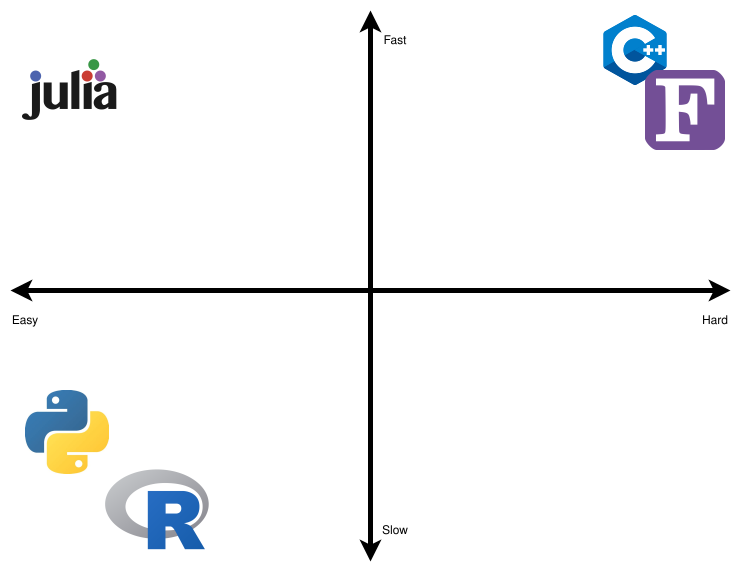
\includegraphics{images/language_comparisons.png}
\caption{Scientific Computing Language Comparisons: logos for FORTRAN,
C++, Python, R and Julia.}\label{fig:language_comparison}
}
\end{figure}

\textbf{Julia is fast! Very fast!} It was designed for speed from the
beginning. In the rest of this section, we go into details about why
this is. If you don't have (much) programming experience yet, feel free
to skip to the next section and maybe come later to this at a later
moment.

Julia accomplishes it's speed partially due to multiple dispatch.
Basically, the idea is to generate very efficient LLVM\footnote{LLVM
  stands for \textbf{L}ow \textbf{L}evel \textbf{V}irtual
  \textbf{M}achine, you can find more at the LLVM website
  (\url{http://llvm.org}).} code. LLVM code, also known as LLVM
instructions, are very low-level, that is, very close to the actual
operations that your computer is executing. So, in essence, Julia
converts your hand written and easy to read code to LLVM machine code
which is very hard for humans to read, but easy for computers to read.
For example, if you define a function taking one argument and pass an
integer into the function, then Julia will create a \emph{specialized}
\passthrough{\lstinline!MethodInstance!}. The next time that you pass an
integer to the function, Julia will look up the
\passthrough{\lstinline!MethodInstance!} that was created earlier and
refer execution to that. Now, the \textbf{great} trick is that you can
also do this inside a function that calls a function. For example, if
some data type is passed into function \passthrough{\lstinline!outer!}
and \passthrough{\lstinline!outer!} calls function
\passthrough{\lstinline!inner!} and the data types passed to
\passthrough{\lstinline!inner!} are known inside the specialized
\passthrough{\lstinline!outer!} instance, then the generated function
\passthrough{\lstinline!inner!} can be hardcoded into function
\passthrough{\lstinline!outer!}! This means that Julia doesn't even have
to lookup \passthrough{\lstinline!MethodInstances!} any more, and the
code can run very efficiently.

Let's show this in practice. We can define the two functions,
\passthrough{\lstinline!inner!}:

\begin{lstlisting}[language=Julia]
inner(x) = x + 3
\end{lstlisting}

and \passthrough{\lstinline!outer!}:

\begin{lstlisting}[language=Julia]
outer(x) = inner(2 * x)
\end{lstlisting}

For example, we can now calculate \passthrough{\lstinline!outer!} for,
let's say, 3:

\begin{lstlisting}[language=Julia]
outer(3)
\end{lstlisting}

\begin{lstlisting}[language=Output]
9
\end{lstlisting}

If you step through this calculation of \passthrough{\lstinline!outer!},
you'll see that the program needs do do quite a lot of things:

\begin{enumerate}
\def\labelenumi{\arabic{enumi}.}
\tightlist
\item
  calculate \passthrough{\lstinline!2 * 3!}
\item
  pass the outcome of \passthrough{\lstinline!2 * 3!} to inner
\item
  calculate
  \passthrough{\lstinline!3 + the outcome of the previous step!}
\end{enumerate}

But, if we ask Julia for the optimized code via
\passthrough{\lstinline!@code\_typed!}, we see what instructions the
computer actually get:

\begin{lstlisting}
@code_llvm debuginfo=:none outer(3)
\end{lstlisting}

\begin{lstlisting}[language=Output]
define i64 @julia_outer_232(i64 signext %0) #0 {
top:
  %1 = shl i64 %0, 1
  %2 = add i64 %1, 3
  ret i64 %2
}
\end{lstlisting}

This is low-level LLVM code showing that the program only does the
following:

\begin{enumerate}
\def\labelenumi{\arabic{enumi}.}
\tightlist
\item
  shift the input (3) one bit to the left, which has the same effect as
  multiplying by 2; and
\item
  add 3.
\end{enumerate}

and that's it! Julia has realized that calling
\passthrough{\lstinline!inner!} can be removed, so that's not part of
the calculation anymore! Now, imagine that this function is called a
thousand or even a million times. These optimizations will reduce the
running time significantly.

The trade-off, here, is that there are cases where earlier assumptions
about the hardcoded \passthrough{\lstinline!MethodInstances!} are
invalidated. Then, the \passthrough{\lstinline!MethodInstance!} has to
be recreated which takes time. Also, the trade-off is that it takes time
to infer what can be hardcoded and what not. This explains why it can
often take very long before Julia does the first thing: in the
background, it is optimizing your code.

So, Julia creates optimized LLVM machine code\footnote{if you like to
  learn more about how Julia is designed you should definitely check
  \protect\hyperlink{ref-bezanson2017julia}{Bezanson et al.}
  (\protect\hyperlink{ref-bezanson2017julia}{2017}).}. You can find
\href{https://julialang.org/benchmarks/}{benchmarks} for Julia and
several other languages here. Figure~\ref{fig:benchmarks} was taken from
\href{https://julialang.org/benchmarks/}{Julia's website benchmarks
section\footnote{please note that the Julia results depicted above do
  not include compile time.}}. As you can see Julia is \textbf{indeed}
fast.

\begin{figure}
\hypertarget{fig:benchmarks}{%
\centering
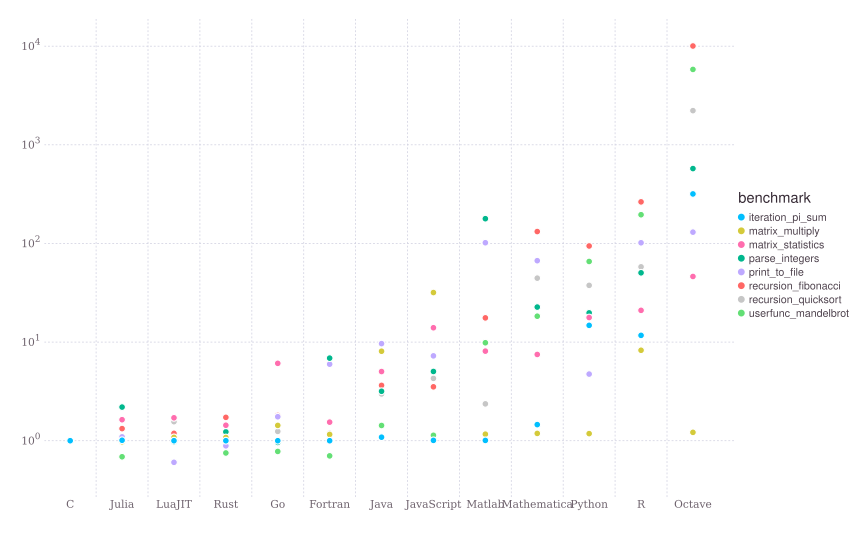
\includegraphics{images/benchmarks.png}
\caption{Julia versus other programming
languages.}\label{fig:benchmarks}
}
\end{figure}

We really believe in Julia. Otherwise, we wouldn't be writing this book.
We think that Julia is the \textbf{future of scientific computing and
scientific data analysis}. It enables the user to develop rapid and
powerful code with a simple syntax. Usually, researchers develop code by
prototyping using a very easy, but slow, language. Once the code is
assured to run correctly and fulfill its goal, then begins the process
of converting the code to a fast, but hard, language. This is known as
the ``Two-Language Problem'' and we discuss next.

\hypertarget{sec:two_language}{%
\subsection{The Two-Language Problem}\label{sec:two_language}}

The ``Two-Language Problem'' is a very typical situation in scientific
computing where a researcher devises an algorithm or a solution to
tackle a desired problem or analysis at hand. Then, the solution is
prototyped in an easy to code language (like Python or R). If the
prototype works, the researcher would code in a fast language that would
not be easy to prototype (C++ or FORTRAN). Thus, we have two languages
involved in the process of developing a new solution. One which is easy
to prototype but is not suited for implementation (mostly due to being
slow). And another which is not so easy to code, and consequently not
easy to prototype, but suited for implementation because it is fast.
Julia avoids such situations by being the \textbf{same language that you
prototype (ease of use) and implement the solution (speed)}.

Also, Julia lets you use \textbf{Unicode characters as variables or
parameters}. This means no more using \passthrough{\lstinline!sigma!} or
\passthrough{\lstinline!sigma\_i!}, and instead just use \(σ\) or \(σᵢ\)
as you would in mathematical notation. When you see code for an
algorithm or for a mathematical equation, you see almost the same
notation and idioms. We call this feature \textbf{``One-To-One Code and
Math Relation''} which is a powerful feature.

We think that the ``Two-Language problem'' and the ``One-To-One Code and
Math Relation'' are best described by one of the creators of Julia, Alan
Edelman, in a \href{https://youtu.be/qGW0GT1rCvs}{TEDx Talk}
(\protect\hyperlink{ref-tedxtalksProgrammingLanguageHeal2020}{TEDx
Talks, 2020}).

\hypertarget{sec:multiple_dispatch}{%
\subsection{Multiple Dispatch}\label{sec:multiple_dispatch}}

Multiple dispatch is a powerful feature that allows us to extend
existing functions or to define custom and complex behavior for new
types. Suppose that you want to define two new
\passthrough{\lstinline!struct!}s to denote two different animals:

\begin{lstlisting}[language=Julia]
abstract type Animal end
struct Fox <: Animal
    weight::Float64
end
struct Chicken <: Animal
    weight::Float64
end
\end{lstlisting}

Basically, this says ``define a fox which is an animal'' and ``define a
chicken which is an animal.'' Next, we might have one fox called Fiona
and a chicken called Big Bird.

\begin{lstlisting}[language=Julia]
fiona = Fox(4.2)
big_bird = Chicken(2.9)
\end{lstlisting}

Next, we want to know how much they weight together, for which we can
write a function:

\begin{lstlisting}[language=Julia]
combined_weight(A1::Animal, A2::Animal) = A1.weight + A2.weight
\end{lstlisting}

\begin{lstlisting}[language=Output]
combined_weight (generic function with 1 method)
\end{lstlisting}

And we want to know whether they go well together. One way to implement
that is to use conditionals:

\begin{lstlisting}[language=Julia]
function naive_trouble(A::Animal, B::Animal)
    if A isa Fox && B isa Chicken
        return true
    elseif A isa Chicken && B isa Fox
        return true
    elseif A isa Chicken && B isa Chicken
        return false
    end
end
\end{lstlisting}

\begin{lstlisting}[language=Output]
naive_trouble (generic function with 1 method)
\end{lstlisting}

Now, let's see whether leaving Fiona and Big Bird together would give
trouble:

\begin{lstlisting}[language=Julia]
naive_trouble(fiona, big_bird)
\end{lstlisting}

\begin{lstlisting}[language=Output]
true
\end{lstlisting}

Okay, so this sounds right. Writing the
\passthrough{\lstinline!naive\_trouble!} function seems to be easy
enough. However, using multiple dispatch to create a new function
\passthrough{\lstinline!trouble!} can have their benefits. Let's create
our new function as follows:

\begin{lstlisting}[language=Julia]
trouble(F::Fox, C::Chicken) = true
trouble(C::Chicken, F::Fox) = true
trouble(C1::Chicken, C2::Chicken) = false
\end{lstlisting}

\begin{lstlisting}[language=Output]
trouble (generic function with 3 methods)
\end{lstlisting}

After defining these methods, \passthrough{\lstinline!trouble!} gives
the same result as \passthrough{\lstinline!naive\_trouble!}. For
example:

\begin{lstlisting}[language=Julia]
trouble(fiona, big_bird)
\end{lstlisting}

\begin{lstlisting}[language=Output]
true
\end{lstlisting}

And leaving Big Bird alone with another chicken called Dora is also fine

\begin{lstlisting}[language=Julia]
dora = Chicken(2.2)
trouble(dora, big_bird)
\end{lstlisting}

\begin{lstlisting}[language=Output]
false
\end{lstlisting}

So, in this case, the benefit of multiple dispatch is that you can just
declare types and Julia will find the correct method for your types.
Even more so, for many cases when multiple dispatch is used inside code,
the Julia compiler will actually optimize the function calls away. For
example, we could write:

\begin{lstlisting}
function trouble(A::Fox, B::Chicken, C::Chicken)
    return trouble(A, B) || trouble(B, C) || trouble(C, A)
end
\end{lstlisting}

Depending on the context, Julia can optimize this to:

\begin{lstlisting}
function trouble(A::Fox, B::Chicken, C::Chicken)
    return true || false || true
end
\end{lstlisting}

because the compiler \textbf{knows} that \passthrough{\lstinline!A!} is
a Fox, \passthrough{\lstinline!B!} is a chicken and so this can be
replaced by the contents of the method
\passthrough{\lstinline!trouble(F::Fox, C::Chicken)!}. The same holds
for \passthrough{\lstinline!trouble(C1::Chicken, C2::Chicken)!}. Next,
the compiler can optimize this to:

\begin{lstlisting}
function trouble(A::Fox, B::Chicken, C::Chicken)
    return true
end
\end{lstlisting}

Another benefit of multiple dispatch is that when someone else now comes
by and wants to compare the existing animals to their animal, a Zebra,
then that's possible. In their package, they can define a Zebra:

\begin{lstlisting}[language=Julia]
struct Zebra <: Animal
    weight::Float64
end
\end{lstlisting}

and also how the interactions with the existing animals would go:

\begin{lstlisting}[language=Julia]
trouble(F::Fox, Z::Zebra) = false
trouble(Z::Zebra, F::Fox) = false
trouble(C::Chicken, Z::Zebra) = false
trouble(Z::Zebra, F::Fox) = false
\end{lstlisting}

\begin{lstlisting}[language=Output]
trouble (generic function with 6 methods)
\end{lstlisting}

Now, we can see whether Marty (our zebra) is safe with Big Bird:

\begin{lstlisting}[language=Julia]
marty = Zebra(412)
trouble(big_bird, marty)
\end{lstlisting}

\begin{lstlisting}[language=Output]
false
\end{lstlisting}

Even better, we can also calculate \textbf{the combined weight of
zebra's and other animals without defining any extra function at our
side}:

\begin{lstlisting}[language=Julia]
combined_weight(big_bird, marty)
\end{lstlisting}

\begin{lstlisting}[language=Output]
414.9
\end{lstlisting}

So, in summary, the code that was written with only Fox and Chicken in
mind works even for types that it \textbf{has never seen before}! In
practice, this means that Julia makes it often easy to re-use code from
other projects.

If you are excited as much as we are by multiple dispatch, here are two
more in-depth examples. The first is a
\href{https://storopoli.io/Bayesian-Julia/pages/1_why_Julia/\#example_one-hot_vector}{fast
and elegant implementation of a one-hot vector} by
\protect\hyperlink{ref-storopoli2021bayesianjulia}{Storopoli}
(\protect\hyperlink{ref-storopoli2021bayesianjulia}{2021}). The second
is an interview with \href{https://www.chrisrackauckas.com/}{Christopher
Rackauckas} at \href{https://youtu.be/moyPIhvw4Nk?t=2107}{Tanmay Bakshi
YouTube's Channel} (see from time 35:07 onwards)
(\protect\hyperlink{ref-tanmaybakshiBakingKnowledgeMachine2021}{tanmay
bakshi, 2021}). Chris mentions that, while using
\href{https://diffeq.sciml.ai/dev/}{\passthrough{\lstinline!DifferentialEquations.jl!}},
a package that he developed and currently maintains, a user filed an
issue that his GPU-based quaternion ODE solver didn't work. Chris was
quite surprised by this request since he would never have expected that
someone would combine GPU computations with quaternions and solving
ODEs. He was even more surprised to discover that the user made a small
mistake and that it all worked. Most of the merit is due to multiple
dispatch and high user code/type sharing.

To conclude, we think that multiple dispatch is best explained by one of
the creators of Julia: \href{https://youtu.be/kc9HwsxE1OY}{Stefan
Karpinski at JuliaCon 2019}.

\hypertarget{sec:julia_wild}{%
\section{Julia in the Wild}\label{sec:julia_wild}}

In Section~\ref{sec:julia_accomplish}, we explained why we think Julia
is such a unique programming language. We showed simple examples about
the main features of Julia. If you would like to have a deep dive on how
Julia is being used, we have some \textbf{interesting use cases}:

\begin{enumerate}
\def\labelenumi{\arabic{enumi}.}
\tightlist
\item
  NASA uses Julia in a supercomputer to analyze the
  \href{https://exoplanets.nasa.gov/news/1669/seven-rocky-trappist-1-planets-may-be-made-of-similar-stuff/}{``Largest
  Batch of Earth-Sized Planets Ever Found''} and achieve a whopping
  \textbf{1,000x speedup} to catalog 188 million astronomical objects in
  15 minutes.
\item
  \href{https://clima.caltech.edu/}{The Climate Modeling Alliance
  (CliMa)} is using mostly Julia to \textbf{model climate in the GPU and
  CPU}. Launched in 2018 in collaboration with researchers at Caltech,
  the NASA Jet Propulsion Laboratory, and the Naval Postgraduate School,
  CliMA is utilizing recent progress in computational science to develop
  an Earth system model that can predict droughts, heat waves, and
  rainfall with unprecedented precision and speed.
\item
  \href{https://youtu.be/19zm1Fn0S9M}{US Federal Aviation Administration
  (FAA) is developing an \textbf{Airborne Collision Avoidance System
  (ACAS-X)} using Julia}. This is a nice example of the ``Two-Language
  Problem'' (see Section~\ref{sec:julia_accomplish}). Previous solutions
  used Matlab to develop the algorithms and C++ for a fast
  implementation. Now, FAA is using one language to do all this: Julia.
\item
  \href{https://juliacomputing.com/case-studies/pfizer/}{\textbf{175x
  speedup} for Pfizer's pharmacology models using GPUs in Julia}. It was
  presented as a
  \href{https://chrisrackauckas.com/assets/Posters/ACoP11_Poster_Abstracts_2020.pdf}{poster}
  in the 11th American Conference of Pharmacometrics (ACoP11) and
  \href{https://web.archive.org/web/20210121164011/https://www.go-acop.org/abstract-awards}{won
  a quality award}.
\item
  \href{https://discourse.julialang.org/t/julia-and-the-satellite-amazonia-1/57541}{The
  Attitude and Orbit Control Subsystem (AOCS) of the Brazilian satellite
  Amazonia-1 is \textbf{written 100\% in Julia}} by Ronan Arraes Jardim
  Chagas (\url{https://ronanarraes.com/}).
\item
  \href{https://youtu.be/NY0HcGqHj3g}{Brazil's national development bank
  (BNDES) ditched a paid solution and opted for open-source Julia
  modeling and gained a \textbf{10x speedup}.}
\end{enumerate}

If this is not enough, there are more case studies in
\href{https://juliacomputing.com/case-studies/}{Julia Computing
website}.

\hypertarget{sec:julia_basics}{%
\chapter{Julia Basics}\label{sec:julia_basics}}

\begin{quote}
\textbf{\emph{NOTE:}} In this chapter we cover the basics of Julia as a
programming language. Please note that this is not \emph{strictly
necessary} for you to use Julia as a tool for data manipulation and data
visualization. Having a basic understanding of Julia will definitely
make you more \emph{effective} and \emph{efficient} in using Julia.
However, if you prefer to get started straight away, you can jump to
Section~\ref{sec:dataframes} to learn about tabular data with
\passthrough{\lstinline!DataFrames.jl!}.
\end{quote}

This is going to be a very brief and \emph{not} an in-depth overview of
the Julia language. If you are already familiar and comfortable with
other programming languages, we highly encourage you to read Julia's
documentation (\url{https://docs.julialang.org/}). The docs are an
excellent resource for taking a deep dive into Julia. It covers all the
basics and corner cases, but it can be cumbersome, especially if you
aren't familiar with software documentation.

We'll cover the basics of Julia. Imagine that Julia is a fancy
feature-loaded car, such as a brand-new Tesla. We'll just explain to you
how to ``drive the car, park it, and how to navigate in traffic.'' If
you want to know what ``all the buttons in the steering wheel and
dashboard do,'' this is not the resource you are looking for.

\hypertarget{sec:ide}{%
\section{Development Environments}\label{sec:ide}}

Before we can dive into the language syntax, we need to answer how to
run code. Going into details about the various options is out of scope
for this book. Instead, we will provide you with some pointers to
various solutions.

The simplest way is to use the Julia REPL. This means starting the Julia
executable (\passthrough{\lstinline!julia!} or
\passthrough{\lstinline!julia.exe!}) and running code there. For
example, we can start the REPL and execute some code:

\begin{lstlisting}
julia> x = 2
2

julia> x + 1
3
\end{lstlisting}

This works all very well, but what if we want to save the code that we
wrote? To save our code, one can write ``.jl'' files such as
``script.jl'' and load these into Julia. Say, that ``script.jl''
contains:

\begin{lstlisting}
x = 3
y = 4
\end{lstlisting}

We can load this into Julia:

\begin{lstlisting}
julia> include("script.jl")

julia> y
4
\end{lstlisting}

Now the problem becomes that we would like Julia to re-read our script
every time before executing code. This can be done via
\href{https://github.com/timholy/Revise.jl}{Revise.jl}. Because
compilation time in Julia is often long,
\passthrough{\lstinline!Revise.jl!} is a must-have for Julia
development. For more information, see the
\passthrough{\lstinline!Revise.jl!} documentation or simply Google a bit
if you have specific questions.

We are aware that \passthrough{\lstinline!Revise.jl!} and the REPL
requires some manual actions which aren't super clearly documented.
Luckily, there is \href{https://github.com/fonsp/Pluto.jl}{Pluto.jl}.
\passthrough{\lstinline!Pluto.jl!} automatically manages dependencies,
runs code, and \textbf{reacts} to changes. For people who are new to
programming, \passthrough{\lstinline!Pluto.jl!} is by far the easiest
way to get started. The main drawback of the package is that it is less
suitable for larger projects.

Other options are to use Visual Studio Code with various Julia
extensions or manage your own IDE. If you \textbf{don't} know what an
IDE is, but do want to manage large projects choose Visual Studio Code.
If you \textbf{do} know what an IDE is, then you might like building
your own IDE with Vim or Emacs and the REPL.

So, to summarize:

\begin{itemize}
\tightlist
\item
  Easiest way to get started -\textgreater{}
  \passthrough{\lstinline!Pluto.jl!}
\item
  Larger projects -\textgreater{} Visual Studio Code
\item
  Advanced users -\textgreater{} Vim, Emacs and the REPL
\end{itemize}

\hypertarget{sec:syntax}{%
\section{Language Syntax}\label{sec:syntax}}

Julia is a \textbf{dynamic-typed language} with a just-in-time compiler.
This means that you don't need to compile your program before you run
it, like you would do in C++ or FORTRAN. Instead, Julia will take your
code, guess types where necessary, and compile parts of code just before
running it. Also, you don't need to explicitly specify each type. Julia
will guess types for you on the go.

The main differences between Julia and other dynamic languages such as R
and Python are the following. First, Julia \textbf{allows the user to
specify type declarations}. You already saw some types declarations in
\emph{Why Julia?} (Section~\ref{sec:why_julia}): they are those double
colons \passthrough{\lstinline!::!} that sometimes come after variables.
However, if you don't want to specify the type of your variables or
functions, Julia will gladly infer (guess) them for you.

Second, Julia allows users to define function behavior across many
combinations of argument types via multiple dispatch. We also covered
multiple dispatch in Section~\ref{sec:julia_accomplish}. We defined a
different type behavior by defining new function signatures for argument
types while using the same function name.

\hypertarget{sec:variable}{%
\subsection{Variables}\label{sec:variable}}

Variables are values that you tell the computer to store with a specific
name, so that you can later recover or change its value. Julia has
several types of variables but, in data science, we mostly use:

\begin{itemize}
\tightlist
\item
  Integers: \passthrough{\lstinline!Int64!}
\item
  Real Numbers: \passthrough{\lstinline!Float64!}
\item
  Boolean: \passthrough{\lstinline!Bool!}
\item
  Strings: \passthrough{\lstinline!String!}
\end{itemize}

Integers and real numbers are stored by using 64 bits by default, that's
why they have the \passthrough{\lstinline!64!} suffix in the name of the
type. If you need more or less precision, there are
\passthrough{\lstinline!Int8!} or \passthrough{\lstinline!Int128!}
types, for example, where higher means more precision. Most of the time,
this won't be an issue so you can just stick to the defaults.

We create new variables by writing the variable name on the left and its
value in the right, and in the middle we use the
\passthrough{\lstinline!=!} assignment operator. For example:

\begin{lstlisting}[language=Julia]
name = "Julia"
age = 9
\end{lstlisting}

\begin{lstlisting}[language=Output]
9
\end{lstlisting}

Note that the return output of the last statement
(\passthrough{\lstinline!age!}) was printed to the console. Here, we are
defining two new variables: \passthrough{\lstinline!name!} and
\passthrough{\lstinline!age!}. We can recover their values by typing the
names given in the assignment:

\begin{lstlisting}[language=Julia]
name
\end{lstlisting}

\begin{lstlisting}[language=Output]
Julia
\end{lstlisting}

If you want to define new values for an existing variable, you can
repeat the steps in the assignment. Note that Julia will now override
the previous value with the new one. Supposed, Julia's birthday has
passed and now it has turned 10:

\begin{lstlisting}[language=Julia]
age = 10
\end{lstlisting}

\begin{lstlisting}[language=Output]
10
\end{lstlisting}

We can do the same with its \passthrough{\lstinline!name!}. Suppose that
Julia has earned some titles due to its blazing speed. We would change
the variable \passthrough{\lstinline!name!} to the new value:

\begin{lstlisting}[language=Julia]
name = "Julia Rapidus"
\end{lstlisting}

\begin{lstlisting}[language=Output]
Julia Rapidus
\end{lstlisting}

We can also do operations on variables such as addition or division.
Let's see how old Julia is, in months, by multiplying
\passthrough{\lstinline!age!} by 12:

\begin{lstlisting}[language=Julia]
12 * age
\end{lstlisting}

\begin{lstlisting}[language=Output]
120
\end{lstlisting}

We can inspect the types of variables by using the
\passthrough{\lstinline!typeof!} function:

\begin{lstlisting}[language=Julia]
typeof(age)
\end{lstlisting}

\begin{lstlisting}[language=Output]
Int64
\end{lstlisting}

The next question then becomes: ``What else can I do with integers?''
There is a nice handy function \passthrough{\lstinline!methodswith!}
that spits out every function available, along with its signature, for a
certain type. Here, I will restrict the output to the first 5 rows:

\begin{lstlisting}[language=Julia]
first(methodswith(Int64), 5)
\end{lstlisting}

\begin{lstlisting}[language=Output]
[1] logmvbeta(p::Int64, a::T, b::T) where T<:Real in StatsFuns at /home/runner/.julia/packages/StatsFuns/vxSkw/src/misc.jl:22
[2] logmvbeta(p::Int64, a::Real, b::Real) in StatsFuns at /home/runner/.julia/packages/StatsFuns/vxSkw/src/misc.jl:23
[3] logmvgamma(p::Int64, a::Real) in StatsFuns at /home/runner/.julia/packages/StatsFuns/vxSkw/src/misc.jl:8
[4] read(t::HTTP.ConnectionPool.Transaction, nb::Int64) in HTTP.ConnectionPool at /home/runner/.julia/packages/HTTP/aTjcj/src/ConnectionPool.jl:232
[5] write(ctx::MbedTLS.MD, i::Union{Float16, Float32, Float64, Int128, Int16, Int32, Int64, UInt128, UInt16, UInt32, UInt64}) in MbedTLS at /home/runner/.julia/packages/MbedTLS/4YY6E/src/md.jl:140
\end{lstlisting}

\hypertarget{sec:struct}{%
\subsection{User-defined Types}\label{sec:struct}}

Having variables around without any sort of hierarchy or relationships
is not ideal. In Julia, we can define that kind of structured data with
a \passthrough{\lstinline!struct!} (also known as a composite type).
Inside each \passthrough{\lstinline!struct!}, you can specify a set of
fields. They differ from the primitive types (e.g.~integer and floats)
that are by default defined already inside the core of Julia language.
Since most \passthrough{\lstinline!struct!}s are user-defined, they are
known as user-defined types.

For example, let's create a \passthrough{\lstinline!struct!} to
represent scientific open source programming languages. We'll also
define a set of fields along with the corresponding types inside the
\passthrough{\lstinline!struct!}:

\begin{lstlisting}[language=Julia]
struct Language
    name::String
    title::String
    year_of_birth::Int64
    fast::Bool
end
\end{lstlisting}

To inspect the field names you can use the
\passthrough{\lstinline!fieldnames!} and pass the desired
\passthrough{\lstinline!struct!} as an argument:

\begin{lstlisting}[language=Julia]
fieldnames(Language)
\end{lstlisting}

\begin{lstlisting}[language=Output]
(:name, :title, :year_of_birth, :fast)
\end{lstlisting}

To use \passthrough{\lstinline!struct!}s, we must instantiate individual
instances (or ``objects''), each with its own specific values for the
fields defined inside the \passthrough{\lstinline!struct!}. Let's
instantiate two instances, one for Julia and one for Python:

\begin{lstlisting}[language=Julia]
julia = Language("Julia", "Rapidus", 2012, true)
python = Language("Python", "Letargicus", 1991, false)
\end{lstlisting}

\begin{lstlisting}[language=Output]
Language("Python", "Letargicus", 1991, false)
\end{lstlisting}

One thing to note with \passthrough{\lstinline!struct!}s is that we
can't change their values once they are instantiated. We can solve this
with a \passthrough{\lstinline!mutable struct!}. Also, note that mutable
objects will, generally, be slower and more error prone. Whenever
possible, make everything \emph{immutable}. Let's create a
\passthrough{\lstinline!mutable struct!}.

\begin{lstlisting}[language=Julia]
mutable struct MutableLanguage
    name::String
    title::String
    year_of_birth::Int64
    fast::Bool
end

julia_mutable = MutableLanguage("Julia", "Rapidus", 2012, true)
\end{lstlisting}

\begin{lstlisting}[language=Output]
MutableLanguage("Julia", "Rapidus", 2012, true)
\end{lstlisting}

Suppose that we want to change
\passthrough{\lstinline!julia\_mutable!}'s title. Now, we can do this
since \passthrough{\lstinline!julia\_mutable!} is an instantiated
\passthrough{\lstinline!mutable struct!}:

\begin{lstlisting}[language=Julia]
julia_mutable.title = "Python Obliteratus"

julia_mutable
\end{lstlisting}

\begin{lstlisting}[language=Output]
MutableLanguage("Julia", "Python Obliteratus", 2012, true)
\end{lstlisting}

\hypertarget{boolean-operators-and-numeric-comparisons}{%
\subsection{Boolean Operators and Numeric
Comparisons}\label{boolean-operators-and-numeric-comparisons}}

Now that we've covered types, we can move to boolean operators and
numeric comparison.

We have three boolean operators in Julia:

\begin{itemize}
\tightlist
\item
  \passthrough{\lstinline"!"}: \textbf{NOT}
\item
  \passthrough{\lstinline!\&\&!}: \textbf{AND}
\item
  \passthrough{\lstinline!||!}: \textbf{OR}
\end{itemize}

Here are a few examples with some of them:

\begin{lstlisting}[language=Julia]
!true
\end{lstlisting}

\begin{lstlisting}[language=Output]
false
\end{lstlisting}

\begin{lstlisting}[language=Julia]
(false && true) || (!false)
\end{lstlisting}

\begin{lstlisting}[language=Output]
true
\end{lstlisting}

\begin{lstlisting}[language=Julia]
(6 isa Int64) && (6 isa Real)
\end{lstlisting}

\begin{lstlisting}[language=Output]
true
\end{lstlisting}

Regarding numeric comparison, Julia has three major types of
comparisons:

\begin{enumerate}
\def\labelenumi{\arabic{enumi}.}
\tightlist
\item
  \textbf{Equality}: either something is \emph{equal} or \emph{not
  equal} another

  \begin{itemize}
  \tightlist
  \item
    == ``equal''
  \item
    != or ≠ ``not equal''
  \end{itemize}
\item
  \textbf{Less than}: either something is \emph{less than} or \emph{less
  than or equal to}

  \begin{itemize}
  \tightlist
  \item
    \textless{} ``less than''
  \item
    \textless= or ≤ ``less than or equal to''
  \end{itemize}
\item
  \textbf{Greater than}: either something is \emph{greater than} or
  \emph{greater than or equal to}

  \begin{itemize}
  \tightlist
  \item
    \textgreater{} ``greater than''
  \item
    \textgreater= or ≥ ``greater than or equal to''
  \end{itemize}
\end{enumerate}

Here are some examples:

\begin{lstlisting}[language=Julia]
1 == 1
\end{lstlisting}

\begin{lstlisting}[language=Output]
true
\end{lstlisting}

\begin{lstlisting}[language=Julia]
1 >= 10
\end{lstlisting}

\begin{lstlisting}[language=Output]
false
\end{lstlisting}

It evens works between different types:

\begin{lstlisting}[language=Julia]
1 == 1.0
\end{lstlisting}

\begin{lstlisting}[language=Output]
true
\end{lstlisting}

We can also mix and match boolean operators with numeric comparisons:

\begin{lstlisting}[language=Julia]
(1 != 10) || (3.14 <= 2.71)
\end{lstlisting}

\begin{lstlisting}[language=Output]
true
\end{lstlisting}

\hypertarget{sec:function}{%
\subsection{Functions}\label{sec:function}}

Now that we already know how to define variables and custom types as
\passthrough{\lstinline!struct!}s, let's turn our attention to
\textbf{functions}. In Julia, a function \textbf{maps argument's values
to one or more return values}. The basic syntax goes like this:

\begin{lstlisting}
function function_name(arg1, arg2)
    result = stuff with the arg1 and arg2
    return result
end
\end{lstlisting}

The function declaration begins with the keyword
\passthrough{\lstinline!function!} followed by the function name. Then,
inside parentheses \passthrough{\lstinline!()!}, we define the arguments
separated by a comma \passthrough{\lstinline!,!}. Inside the function,
we specify what we want Julia to do with the parameters that we
supplied. All variables that we define inside a function are deleted
after the function returns. This is nice because it is like an automatic
cleanup. After all the operations in the function body are finished, we
instruct Julia to return the final result with the
\passthrough{\lstinline!return!} statement. Finally, we let Julia know
that the function definition is finished with the
\passthrough{\lstinline!end!} keyword.

There is also the compact \textbf{assignment form}:

\begin{lstlisting}
f_name(arg1, arg2) = stuff with the arg1 and arg2
\end{lstlisting}

It is the \textbf{same function} as before but with a different, more
compact, form. As a rule of thumb, when your code can fit easily on one
line of up to 92 characters, then the compact form is suitable.
Otherwise, just use the longer form with the
\passthrough{\lstinline!function!} keyword. Let's dive into some
examples.

\hypertarget{sec:function_example}{%
\subsubsection{Creating new Functions}\label{sec:function_example}}

Let's create a new function that adds numbers together:

\begin{lstlisting}[language=Julia]
function add_numbers(x, y)
    return x + y
end
\end{lstlisting}

\begin{lstlisting}[language=Output]
add_numbers (generic function with 1 method)
\end{lstlisting}

Now, we can use our \passthrough{\lstinline!add\_numbers!} function:

\begin{lstlisting}[language=Julia]
add_numbers(17, 29)
\end{lstlisting}

\begin{lstlisting}[language=Output]
46
\end{lstlisting}

And it works also with floats:

\begin{lstlisting}[language=Julia]
add_numbers(3.14, 2.72)
\end{lstlisting}

\begin{lstlisting}[language=Output]
5.86
\end{lstlisting}

Also, we can define custom behavior by specifying type declarations.
Suppose that we want to have a \passthrough{\lstinline!round\_number!}
function that behaves differently if its argument is either a
\passthrough{\lstinline!Float64!} or \passthrough{\lstinline!Int64!}:

\begin{lstlisting}[language=Julia]
function round_number(x::Float64)
    return round(x)
end

function round_number(x::Int64)
    return x
end
\end{lstlisting}

\begin{lstlisting}[language=Output]
round_number (generic function with 2 methods)
\end{lstlisting}

We can see that it is a function with multiple methods:

\begin{lstlisting}[language=Julia]
methods(round_number)
\end{lstlisting}

\begin{lstlisting}[language=Output]
round_number(x::Float64) in Main at none:1
\end{lstlisting}

\begin{lstlisting}[language=Output]
round_number(x::Int64) in Main at none:5
\end{lstlisting}

There is one issue: what happens if we want to round a 32-bit float
\passthrough{\lstinline!Float32!}? Or a 8-bit integer
\passthrough{\lstinline!Int8!}?

If you want something to function on all float and integer types, you
can use an \textbf{abstract type} as the type signature, such as
\passthrough{\lstinline!AbstractFloat!} or
\passthrough{\lstinline!Integer!}:

\begin{lstlisting}[language=Julia]
function round_number(x::AbstractFloat)
    return round(x)
end
\end{lstlisting}

\begin{lstlisting}[language=Output]
round_number (generic function with 3 methods)
\end{lstlisting}

Now, it works as expected with any float type:

\begin{lstlisting}[language=Julia]
x_32 = Float32(1.1)
round_number(x_32)
\end{lstlisting}

\begin{lstlisting}[language=Output]
1.0f0
\end{lstlisting}

\begin{quote}
\textbf{\emph{NOTE:}} We can inspect types with the
\passthrough{\lstinline!supertypes!} and
\passthrough{\lstinline!subtypes!} functions.
\end{quote}

Let's go back to our \passthrough{\lstinline!Language!}
\passthrough{\lstinline!struct!} that we defined above. This is an
example of multiple dispatch. We will extend the
\passthrough{\lstinline!Base.show!} function that prints the output of
instantiated types and \passthrough{\lstinline!struct!}s.

By default, a \passthrough{\lstinline!struct!} has a basic output, which
you saw above in the \passthrough{\lstinline!python!} case. We can
define a new \passthrough{\lstinline!Base.show!} method to our
\passthrough{\lstinline!Language!} type, so that we have some nice
printing for our programming languages instances. We want to clearly
communicate programming languages' names, titles, and ages in years. The
function \passthrough{\lstinline!Base.show!} accepts as arguments a
\passthrough{\lstinline!IO!} type named \passthrough{\lstinline!io!}
followed by the type you want to define custom behavior:

\begin{lstlisting}[language=Julia]
Base.show(io::IO, l::Language) = print(
    io, l.name, ", ",
    2021 - l.year_of_birth, " years old, ",
    "has the following titles: ", l.title
)
\end{lstlisting}

Now, let's see how \passthrough{\lstinline!python!} will output:

\begin{lstlisting}[language=Julia]
python
\end{lstlisting}

\begin{lstlisting}[language=Output]
Python, 30 years old, has the following titles: Letargicus
\end{lstlisting}

\hypertarget{sec:function_multiple}{%
\subsubsection{Multiple Return Values}\label{sec:function_multiple}}

A function can, also, return two or more values. See the new function
\passthrough{\lstinline!add\_multiply!} below:

\begin{lstlisting}[language=Julia]
function add_multiply(x, y)
    addition = x + y
    multiplication = x * y
    return addition, multiplication
end
\end{lstlisting}

\begin{lstlisting}[language=Output]
add_multiply (generic function with 1 method)
\end{lstlisting}

In that case, we can do two things:

\begin{enumerate}
\def\labelenumi{\arabic{enumi}.}
\item
  We can, analogously as the return values, define two variables to hold
  the function return values, one for each return value:

  \begin{lstlisting}[language=Julia]
  return_1, return_2 = add_multiply(1, 2)
  return_2
  \end{lstlisting}

  \begin{lstlisting}[language=Output]
  2
  \end{lstlisting}
\item
  Or we can define just one variable to hold the function's return
  values and access them with either \passthrough{\lstinline!first!} or
  \passthrough{\lstinline!last!}:

  \begin{lstlisting}[language=Julia]
  all_returns = add_multiply(1, 2)
  last(all_returns)
  \end{lstlisting}

  \begin{lstlisting}[language=Output]
  2
  \end{lstlisting}
\end{enumerate}

\hypertarget{sec:function_keyword_arguments}{%
\subsubsection{Keyword Arguments}\label{sec:function_keyword_arguments}}

Some functions can accept keyword arguments instead of positional
arguments. These arguments are just like regular arguments, except that
they are defined after the regular function's arguments and separated by
a semicolon \passthrough{\lstinline!;!}. For example, let's define a
\passthrough{\lstinline!logarithm!} function that by default uses base
\(e\) (2.718281828459045) as a keyword argument. Note that, here, we are
using the abstract type \passthrough{\lstinline!Real!} so that we cover
all types derived from \passthrough{\lstinline!Integer!} and
\passthrough{\lstinline!AbstractFloat!}, being both themselves subtypes
of \passthrough{\lstinline!Real!}:

\begin{lstlisting}[language=Julia]
AbstractFloat <: Real && Integer <: Real
\end{lstlisting}

\begin{lstlisting}[language=Output]
true
\end{lstlisting}

\begin{lstlisting}[language=Julia]
function logarithm(x::Real; base::Real=2.7182818284590)
    return log(base, x)
end
\end{lstlisting}

\begin{lstlisting}[language=Output]
logarithm (generic function with 1 method)
\end{lstlisting}

It works without specifying the \passthrough{\lstinline!base!} argument
as we supplied a \textbf{default argument value} in the function
declaration:

\begin{lstlisting}[language=Julia]
logarithm(10)
\end{lstlisting}

\begin{lstlisting}[language=Output]
2.3025850929940845
\end{lstlisting}

And also with the keyword argument \passthrough{\lstinline!base!}
different from its default value:

\begin{lstlisting}[language=Julia]
logarithm(10; base=2)
\end{lstlisting}

\begin{lstlisting}[language=Output]
3.3219280948873626
\end{lstlisting}

\hypertarget{sec:function_anonymous}{%
\subsubsection{Anonymous Functions}\label{sec:function_anonymous}}

Often we don't care about the name of the function and want to quickly
make one. What we need are \textbf{anonymous functions}. They are used a
lot in Julia's data science workflow. For example, when using
\passthrough{\lstinline!DataFrames.jl!} (Section~\ref{sec:dataframes})
or \passthrough{\lstinline!Makie.jl!}
(Section~\ref{sec:DataVisualizationMakie}), sometimes we need a
temporary function to filter data or format plot labels. That's when we
use anonymous functions. They are especially useful when we don't want
to create a function, and a simple in-place statement would be enough.

The syntax is simple. We use the \passthrough{\lstinline!->!} operator.
On the left of \passthrough{\lstinline!->!} we define the parameter
name. And on the right of \passthrough{\lstinline!->!} we define what
operations we want to perform on the parameter that we defined on the
left of \passthrough{\lstinline!->!}. Here is an example. Suppose that
we want to undo the log transformation by using an exponentiation:

\begin{lstlisting}[language=Julia]
map(x -> 2.7182818284590^x, logarithm(2))
\end{lstlisting}

\begin{lstlisting}[language=Output]
2.0
\end{lstlisting}

Here, we are using the \passthrough{\lstinline!map!} function to
conveniently map the anonymous function (first argument) to
\passthrough{\lstinline!logarithm(2)!} (the second argument). As a
result, we get back the same number, because logarithm and
exponentiation are inverse (at least in the base that we've chosen --
2.7182818284590)

\hypertarget{sec:conditionals}{%
\subsection{Conditional If-Else-Elseif}\label{sec:conditionals}}

In most programming languages, the user is allowed to control the
computer's flow of execution. Depending on the situation, we want the
computer to do one thing or another. In Julia we can control the flow of
execution with \passthrough{\lstinline!if!},
\passthrough{\lstinline!elseif!}, and \passthrough{\lstinline!else!}
keywords. These are known as conditional statements.

The \passthrough{\lstinline!if!} keyword prompts Julia to evaluate an
expression and, depending on whether it's \passthrough{\lstinline!true!}
or \passthrough{\lstinline!false!}, execute certain portions of code. We
can compound several \passthrough{\lstinline!if!} conditions with the
\passthrough{\lstinline!elseif!} keyword for complex control flow.
Finally, we can define an alternative portion to be executed if anything
inside the \passthrough{\lstinline!if!} or
\passthrough{\lstinline!elseif!}s is evaluated to
\passthrough{\lstinline!true!}. This is the purpose of the
\passthrough{\lstinline!else!} keyword. Finally, like all the previous
keyword operators that we saw, we must tell Julia when the conditional
statement is finished with the \passthrough{\lstinline!end!} keyword.

Here's an example with all the
\passthrough{\lstinline!if!}-\passthrough{\lstinline!elseif!}-\passthrough{\lstinline!else!}
keywords:

\begin{lstlisting}[language=Julia]
a = 1
b = 2

if a < b
    "a is less than b"
elseif a > b
    "a is greater than b"
else
    "a is equal to b"
end
\end{lstlisting}

\begin{lstlisting}[language=Output]
a is less than b
\end{lstlisting}

We can even wrap this in a function called
\passthrough{\lstinline!compare!}:

\begin{lstlisting}[language=Julia]
function compare(a, b)
    if a < b
        "a is less than b"
    elseif a > b
        "a is greater than b"
    else
        "a is equal to b"
    end
end

compare(3.14, 3.14)
\end{lstlisting}

a is equal to b

\hypertarget{sec:for}{%
\subsection{For Loop}\label{sec:for}}

The classical for loop in Julia follows a similar syntax as the
conditional statements. You begin with a keyword, in this case
\passthrough{\lstinline!for!}. Then, you specify what Julia should
``loop'' for, i.e., a sequence. Also, like everything else, you must
finish with the \passthrough{\lstinline!end!} keyword.

So, to make Julia print every number from 1 to 10, you can use the
following for loop:

\begin{lstlisting}[language=Julia]
for i in 1:10
    println(i)
end
\end{lstlisting}

\hypertarget{sec:while}{%
\subsection{While Loop}\label{sec:while}}

The while loop is a mix of the previous conditional statements and for
loops. Here, the loop is executed every time the condition is
\passthrough{\lstinline!true!}. The syntax follows the same form as the
previous one. We begin with the keyword \passthrough{\lstinline!while!},
followed by a statement that evaluates to \passthrough{\lstinline!true!}
or \passthrough{\lstinline!false!}. As usual, you must end with the
\passthrough{\lstinline!end!} keyword.

Here's an example:

\begin{lstlisting}[language=Julia]
n = 0

while n < 3
    global n += 1
end

n
\end{lstlisting}

\begin{lstlisting}[language=Output]
3
\end{lstlisting}

As you can see, we have to use the \passthrough{\lstinline!global!}
keyword. This is because of \textbf{variable scope}. Variables defined
inside conditional statements, loops, and functions exist only inside
them. This is known as the \emph{scope} of the variable. Here, we had to
tell Julia that the \passthrough{\lstinline!n!} inside
\passthrough{\lstinline!while!} loop is in the global scope with the
\passthrough{\lstinline!global!} keyword.

Finally, we also used the \passthrough{\lstinline!+=!} operator which is
a nice shorthand for \passthrough{\lstinline!n = n + 1!}.

\hypertarget{sec:data_structures}{%
\section{Native Data Structures}\label{sec:data_structures}}

Julia has several native data structures. They are abstractions of data
that represent some form of structured data. We will cover the most used
ones. They hold homogeneous or heterogeneous data. Since they are
collections, they can be \emph{looped} over with the
\passthrough{\lstinline!for!} loops.

We will cover \passthrough{\lstinline!String!},
\passthrough{\lstinline!Tuple!}, \passthrough{\lstinline!NamedTuple!},
\passthrough{\lstinline!UnitRange!}, \passthrough{\lstinline!Arrays!},
\passthrough{\lstinline!Pair!}, \passthrough{\lstinline!Dict!},
\passthrough{\lstinline!Symbol!}.

When you stumble across a data structure in Julia, you can find methods
that accept it as an argument with the
\passthrough{\lstinline!methodswith!} function. In Julia, the
distinction between methods and functions is as follows. Every function
can have multiple methods like we have shown earlier. The
\passthrough{\lstinline!methodswith!} function is nice to have in your
bag of tricks. Let's see what we can do with a
\passthrough{\lstinline!String!} for example:

\begin{lstlisting}[language=Julia]
first(methodswith(String), 5)
\end{lstlisting}

\begin{lstlisting}[language=Output]
[1] write(fp::FilePathsBase.SystemPath, x::Union{String, Vector{UInt8}}) in FilePathsBase at /home/runner/.julia/packages/FilePathsBase/dVWLK/src/system.jl:380
[2] write(fp::FilePathsBase.SystemPath, x::Union{String, Vector{UInt8}}, mode) in FilePathsBase at /home/runner/.julia/packages/FilePathsBase/dVWLK/src/system.jl:380
[3] write(iod::HTTP.DebugRequest.IODebug, x::String) in HTTP.DebugRequest at /home/runner/.julia/packages/HTTP/aTjcj/src/IODebug.jl:38
[4] write(buffer::FilePathsBase.FileBuffer, x::String) in FilePathsBase at /home/runner/.julia/packages/FilePathsBase/dVWLK/src/buffer.jl:85
[5] write(io::IO, s::Union{SubString{String}, String}) in Base at strings/io.jl:244
\end{lstlisting}

\hypertarget{sec:broadcasting}{%
\subsection{Broadcasting Operators and
Functions}\label{sec:broadcasting}}

Before we dive into data structures, we need to talk about broadcasting
(also known as \emph{vectorization}) and the ``dot'' operator
\passthrough{\lstinline!.!}.

We can broadcast mathematical operations like
\passthrough{\lstinline!*!} (multiplication) or
\passthrough{\lstinline!+!} (addition) using the dot operator. For
example, broadcasted addition would imply a change from
\passthrough{\lstinline!+!} to \passthrough{\lstinline!.+!}:

\begin{lstlisting}[language=Julia]
[1, 2, 3] .+ 1
\end{lstlisting}

\begin{lstlisting}[language=Output]
[2, 3, 4]
\end{lstlisting}

It also works automatically with functions. (Technically, the
mathematical operations, or infix operators, are also functions, but
that is not so important to know.) Remember our
\passthrough{\lstinline!logarithm!} function?

\begin{lstlisting}[language=Julia]
logarithm.([1, 2, 3])
\end{lstlisting}

\begin{lstlisting}[language=Output]
[0.0, 0.6931471805599569, 1.0986122886681282]
\end{lstlisting}

\hypertarget{sec:function_bang}{%
\subsection{\texorpdfstring{Functions with a bang
\texttt{!}}{Functions with a bang !}}\label{sec:function_bang}}

It is a Julia convention to append a bang \passthrough{\lstinline"!"} to
names of functions that modify one or more of their arguments. This
convention warns the user that the function is \textbf{not pure}, i.e.,
that it has \emph{side effects}. A function with side effects is useful
when you want to update a large data structure or variable container
without having all the overhead from creating a new instance.

For example, we can create a function that adds 1 to each element in a
vector \passthrough{\lstinline!V!}:

\begin{lstlisting}[language=Julia]
function add_one!(V)
    for i in 1:length(V)
        V[i] += 1
    end
    return nothing
end
\end{lstlisting}

\begin{lstlisting}[language=Julia]
my_data = [1, 2, 3]

add_one!(my_data)

my_data
\end{lstlisting}

\begin{lstlisting}[language=Output]
[2, 3, 4]
\end{lstlisting}

\hypertarget{sec:string}{%
\subsection{String}\label{sec:string}}

\textbf{Strings} are represented delimited by double quotes:

\begin{lstlisting}[language=Julia]
typeof("This is a string")
\end{lstlisting}

\begin{lstlisting}[language=Output]
String
\end{lstlisting}

We can also write a multiline string:

\begin{lstlisting}[language=Julia]
text = "
This is a big multiline string.
As you can see.
It is still a String to Julia.
"
\end{lstlisting}

\begin{lstlisting}[language=Output]

This is a big multiline string.
As you can see.
It is still a String to Julia.

\end{lstlisting}

But it is usually clearer to use triple quotation marks:

\begin{lstlisting}[language=Julia]
s = """
    This is a big multiline string with a nested "quotation".
    As you can see.
    It is still a String to Julia.
    """
\end{lstlisting}

\begin{lstlisting}[language=Output]
This is a big multiline string with a nested "quotation".
As you can see.
It is still a String to Julia.

\end{lstlisting}

When using triple-backticks, the indentation and newline at the start is
ignored by Julia. This improves code readability because you can indent
the block in your source code without those spaces ending up in your
string.

\hypertarget{sec:string_concatenation}{%
\subsubsection{String Concatenation}\label{sec:string_concatenation}}

A common string operation is \textbf{string concatenation}. Suppose that
you want to construct a new string that is the concatenation of two or
more strings. This is accomplished in Julia either with the
\passthrough{\lstinline!*!} operator or the
\passthrough{\lstinline!join!} function. This symbol might sound like a
weird choice and it actually is. For now, many Julia codebases are using
this symbol, so it will stay in the language. If you're interested, you
can read a discussion from 2015 about it at
\url{https://github.com/JuliaLang/julia/issues/11030}.

\begin{lstlisting}[language=Julia]
hello = "Hello"
goodbye = "Goodbye"

hello * goodbye
\end{lstlisting}

\begin{lstlisting}[language=Output]
HelloGoodbye
\end{lstlisting}

As you can see, we are missing a space between
\passthrough{\lstinline!hello!} and \passthrough{\lstinline!goodbye!}.
We could concatenate an additional \passthrough{\lstinline!" "!} string
with the \passthrough{\lstinline!*!}, but that would be cumbersome for
more than two strings. That's where the \passthrough{\lstinline!join!}
function comes in handy. We just pass as arguments the strings inside
the brackets \passthrough{\lstinline![]!} and the separator:

\begin{lstlisting}[language=Julia]
join([hello, goodbye], " ")
\end{lstlisting}

\begin{lstlisting}[language=Output]
Hello Goodbye
\end{lstlisting}

\hypertarget{sec:string_interpolation}{%
\subsubsection{String Interpolation}\label{sec:string_interpolation}}

Concatenating strings can be convoluted. We can be much more expressive
with \textbf{string interpolation}. It works like this: you specify
whatever you want to be included in your string with the dollar sign
\passthrough{\lstinline!$!}. Here's the example before but now using
interpolation:

\begin{lstlisting}[language=Julia]
"$hello $goodbye"
\end{lstlisting}

\begin{lstlisting}[language=Output]
Hello Goodbye
\end{lstlisting}

It even works inside functions. Let's revisit our
\passthrough{\lstinline!test!} function from
Section~\ref{sec:conditionals}:

\begin{lstlisting}[language=Julia]
function test_interpolated(a, b)
    if a < b
        "$a is less than $b"
    elseif a > b
        "$a is greater than $b"
    else
        "$a is equal to $b"
    end
end

test_interpolated(3.14, 3.14)
\end{lstlisting}

\begin{lstlisting}[language=Output]
3.14 is equal to 3.14
\end{lstlisting}

\hypertarget{sec:string_manipulations}{%
\subsubsection{String Manipulations}\label{sec:string_manipulations}}

There are several functions to manipulate strings in Julia. We will
demonstrate the most common ones. Also, note that most of these
functions accept a
\href{https://docs.julialang.org/en/v1/manual/strings/\#Regular-Expressions}{Regular
Expression (RegEx)} as arguments. We won't cover RegEx in this book, but
you are encouraged to learn about them, especially if most of your work
uses textual data.

First, let us define a string for us to play around with:

\begin{lstlisting}[language=Julia]
julia_string = "Julia is an amazing open source programming language"
\end{lstlisting}

\begin{lstlisting}[language=Output]
Julia is an amazing open source programming language
\end{lstlisting}

\begin{enumerate}
\def\labelenumi{\arabic{enumi}.}
\item
  \passthrough{\lstinline!contains!},
  \passthrough{\lstinline!startswith!} and
  \passthrough{\lstinline!endswith!}: A conditional (returns either
  \passthrough{\lstinline!true!} or \passthrough{\lstinline!false!}) if
  the second argument is a:

  \begin{itemize}
  \item
    \textbf{substring} of the first argument

    \begin{lstlisting}[language=Julia]
    contains(julia_string, "Julia")
    \end{lstlisting}

    \begin{lstlisting}[language=Output]
    true
    \end{lstlisting}
  \item
    \textbf{prefix} of the first argument

    \begin{lstlisting}[language=Julia]
    startswith(julia_string, "Julia")
    \end{lstlisting}

    \begin{lstlisting}[language=Output]
    true
    \end{lstlisting}
  \item
    \textbf{suffix} of the first argument

    \begin{lstlisting}[language=Julia]
    endswith(julia_string, "Julia")
    \end{lstlisting}

    \begin{lstlisting}[language=Output]
    false
    \end{lstlisting}
  \end{itemize}
\item
  \passthrough{\lstinline!lowercase!},
  \passthrough{\lstinline!uppercase!},
  \passthrough{\lstinline!titlecase!} and
  \passthrough{\lstinline!lowercasefirst!}:

  \begin{lstlisting}[language=Julia]
  lowercase(julia_string)
  \end{lstlisting}

  \begin{lstlisting}[language=Output]
  julia is an amazing open source programming language
  \end{lstlisting}

  \begin{lstlisting}[language=Julia]
  uppercase(julia_string)
  \end{lstlisting}

  \begin{lstlisting}[language=Output]
  JULIA IS AN AMAZING OPEN SOURCE PROGRAMMING LANGUAGE
  \end{lstlisting}

  \begin{lstlisting}[language=Julia]
  titlecase(julia_string)
  \end{lstlisting}

  \begin{lstlisting}[language=Output]
  Julia Is An Amazing Open Source Programming Language
  \end{lstlisting}

  \begin{lstlisting}[language=Julia]
  lowercasefirst(julia_string)
  \end{lstlisting}

  \begin{lstlisting}[language=Output]
  julia is an amazing open source programming language
  \end{lstlisting}
\item
  \passthrough{\lstinline!replace!}: introduces a new syntax, called the
  \passthrough{\lstinline!Pair!}

  \begin{lstlisting}[language=Julia]
  replace(julia_string, "amazing" => "awesome")
  \end{lstlisting}

  \begin{lstlisting}[language=Output]
  Julia is an awesome open source programming language
  \end{lstlisting}
\item
  \passthrough{\lstinline!split!}: breaks up a string by a delimiter:

  \begin{lstlisting}[language=Julia]
  split(julia_string, " ")
  \end{lstlisting}

  \begin{lstlisting}[language=Output]
  SubString{String}["Julia", "is", "an", "amazing", "open", "source", "programming", "language"]
  \end{lstlisting}
\end{enumerate}

\hypertarget{sec:string_conversions}{%
\subsubsection{String Conversions}\label{sec:string_conversions}}

Often, we need to \textbf{convert} between types in Julia. To convert a
number to a string we can use the \passthrough{\lstinline!string!}
function:

\begin{lstlisting}[language=Julia]
my_number = 123
typeof(string(my_number))
\end{lstlisting}

\begin{lstlisting}[language=Output]
String
\end{lstlisting}

Sometimes, we want the opposite: convert a string to a number. Julia has
a handy function for that: \passthrough{\lstinline!parse!}.

\begin{lstlisting}[language=Julia]
typeof(parse(Int64, "123"))
\end{lstlisting}

\begin{lstlisting}[language=Output]
Int64
\end{lstlisting}

Sometimes, we want to play safe with these conversions. That's when
\passthrough{\lstinline!tryparse!} function steps in. It has the same
functionality as \passthrough{\lstinline!parse!} but returns either a
value of the requested type, or \passthrough{\lstinline!nothing!}. That
makes \passthrough{\lstinline!tryparse!} handy when we want to avoid
errors. Of course, you would need to deal with all those
\passthrough{\lstinline!nothing!} values afterwards.

\begin{lstlisting}[language=Julia]
tryparse(Int64, "A very non-numeric string")
\end{lstlisting}

\begin{lstlisting}[language=Output]
nothing
\end{lstlisting}

\hypertarget{sec:tuple}{%
\subsection{Tuple}\label{sec:tuple}}

Julia has a data structure called \textbf{tuple}. They are really
\emph{special} in Julia because they are often used in relation to
functions. Since functions are an important feature in Julia, every
Julia user should know the basics of tuples.

A tuple is a \textbf{fixed-length container that can hold multiple
different types}. A tuple is an \textbf{immutable object}, meaning that
it cannot be modified after instantiation. To construct a tuple, use
parentheses \passthrough{\lstinline!()!} to delimit the beginning and
end, along with commas \passthrough{\lstinline!,!} as delimiters between
values:

\begin{lstlisting}[language=Julia]
my_tuple = (1, 3.14, "Julia")
\end{lstlisting}

\begin{lstlisting}[language=Output]
(1, 3.14, "Julia")
\end{lstlisting}

Here, we are creating a tuple with three values. Each one of the values
is a different type. We can access them via indexing. Like this:

\begin{lstlisting}[language=Julia]
my_tuple[2]
\end{lstlisting}

\begin{lstlisting}[language=Output]
3.14
\end{lstlisting}

We can also loop over tuples with the \passthrough{\lstinline!for!}
keyword. And even apply functions to tuples. But we can \textbf{never
change any value of a tuple} since they are \textbf{immutable}.

Remember functions that return multiple values back in
Section~\ref{sec:function_multiple}? Let's inspect what our
\passthrough{\lstinline!add\_multiply!} function returns:

\begin{lstlisting}[language=Julia]
return_multiple = add_multiply(1, 2)
typeof(return_multiple)
\end{lstlisting}

\begin{lstlisting}[language=Output]
Tuple{Int64, Int64}
\end{lstlisting}

This is because \passthrough{\lstinline!return a, b!} is the same as
\passthrough{\lstinline!return (a, b)!}:

\begin{lstlisting}[language=Julia]
1, 2
\end{lstlisting}

\begin{lstlisting}[language=Output]
(1, 2)
\end{lstlisting}

So, now you can see why they are often related.

One more thing about tuples. \textbf{When you want to pass more than one
variable to an anonymous function, guess what you would need to use?
Once again: tuples!}

\begin{lstlisting}[language=Julia]
map((x, y) -> x^y, 2, 3)
\end{lstlisting}

\begin{lstlisting}[language=Output]
8
\end{lstlisting}

Or, even more than two arguments:

\begin{lstlisting}[language=Julia]
map((x, y, z) -> x^y + z, 2, 3, 1)
\end{lstlisting}

\begin{lstlisting}[language=Output]
9
\end{lstlisting}

\hypertarget{sec:namedtuple}{%
\subsection{Named Tuple}\label{sec:namedtuple}}

Sometimes, you want to name the values in tuples. That's when
\textbf{named tuples} comes in. Their functionality is pretty much same
as tuples: they are \textbf{immutable} and can hold \textbf{any type of
value}.

The construction of named tuples is slightly different from that of
tuples. You have the familiar parentheses \passthrough{\lstinline!()!}
and the comma \passthrough{\lstinline!,!} value separator. But now you
\textbf{name the values}:

\begin{lstlisting}[language=Julia]
my_namedtuple = (i=1, f=3.14, s="Julia")
\end{lstlisting}

\begin{lstlisting}[language=Output]
(i = 1, f = 3.14, s = "Julia")
\end{lstlisting}

We can access named tuple's values via indexing like regular tuples or,
alternatively, \textbf{access by their names} with the
\passthrough{\lstinline!.!}:

\begin{lstlisting}[language=Julia]
my_namedtuple.s
\end{lstlisting}

\begin{lstlisting}[language=Output]
Julia
\end{lstlisting}

To finish our discussion of named tuples, there is one important
\emph{quick} syntax that you'll see a lot in Julia code. Often Julia
users create a named tuple by using the familiar parenthesis
\passthrough{\lstinline!()!} and commas \passthrough{\lstinline!,!}, but
without naming the values. To do so you \textbf{begin the named tuple
construction by specifying first a semicolon \passthrough{\lstinline!;!}
before the values}. This is especially useful when the values that would
compose the named tuple are already defined in variables or when you
want to avoid long lines:

\begin{lstlisting}[language=Julia]
i = 1
f = 3.14
s = "Julia"

my_quick_namedtuple = (; i, f, s)
\end{lstlisting}

\begin{lstlisting}[language=Output]
(i = 1, f = 3.14, s = "Julia")
\end{lstlisting}

\hypertarget{sec:ranges}{%
\subsection{Ranges}\label{sec:ranges}}

A \textbf{range} in Julia represents an interval between start and stop
boundaries. The syntax is \passthrough{\lstinline!start:stop!}:

\begin{lstlisting}[language=Julia]
1:10
\end{lstlisting}

\begin{lstlisting}[language=Output]
1:10
\end{lstlisting}

As you can see, our instantiated range is of type
\passthrough{\lstinline!UnitRange\{T\}!} where
\passthrough{\lstinline!T!} is the type inside the
\passthrough{\lstinline!UnitRange!}:

\begin{lstlisting}[language=Julia]
typeof(1:10)
\end{lstlisting}

\begin{lstlisting}[language=Output]
UnitRange{Int64}
\end{lstlisting}

And, if we gather all the values, we get:

\begin{lstlisting}[language=Julia]
[x for x in 1:10]
\end{lstlisting}

\begin{lstlisting}[language=Output]
[1, 2, 3, 4, 5, 6, 7, 8, 9, 10]
\end{lstlisting}

We can also construct ranges for other types:

\begin{lstlisting}[language=Julia]
typeof(1.0:10.0)
\end{lstlisting}

\begin{lstlisting}[language=Output]
StepRangeLen{Float64, Base.TwicePrecision{Float64}, Base.TwicePrecision{Float64}, Int64}
\end{lstlisting}

Sometimes, we want to change the default interval step size behavior. We
can do that by adding a step size in the range syntax
\passthrough{\lstinline!start:step:stop!}. For example, suppose we want
a range of \passthrough{\lstinline!Float64!} from 0 to 1 with steps of
size 0.2:

\begin{lstlisting}[language=Julia]
0.0:0.2:1.0
\end{lstlisting}

\begin{lstlisting}[language=Output]
0.0:0.2:1.0
\end{lstlisting}

If you want to ``materialize'' a range into a collection, you can use
the function \passthrough{\lstinline!collect!}:

\begin{lstlisting}[language=Julia]
collect(1:10)
\end{lstlisting}

\begin{lstlisting}[language=Output]
[1, 2, 3, 4, 5, 6, 7, 8, 9, 10]
\end{lstlisting}

We have an array of the type specified in the range between the
boundaries that we've set. Speaking of arrays, let's talk about them.

\hypertarget{sec:array}{%
\subsection{Array}\label{sec:array}}

In its most basic form, \textbf{array}s hold multiple objects. For
example, they can hold multiple numbers in one-dimension:

\begin{lstlisting}[language=Julia]
myarray = [1, 2, 3]
\end{lstlisting}

\begin{lstlisting}[language=Output]
[1, 2, 3]
\end{lstlisting}

Most of the time you would want \textbf{arrays of a single type for
performance issues}, but note that they can also hold objects of
different types:

\begin{lstlisting}[language=Julia]
myarray = ["text", 1, :symbol]
\end{lstlisting}

\begin{lstlisting}[language=Output]
Any["text", 1, :symbol]
\end{lstlisting}

They are the ``bread and butter'' of data scientist, because arrays are
what underlies most of \textbf{data manipulation} and \textbf{data
visualization} workflows.

Therefore, \textbf{Arrays are an essential data structure}.

\hypertarget{sec:array_types}{%
\subsubsection{Array Types}\label{sec:array_types}}

Let's start with \textbf{array types}. There are several, but we will
focus on the two most used in data science:

\begin{itemize}
\tightlist
\item
  \passthrough{\lstinline!Vector\{T\}!}: \textbf{one-dimensional} array.
  Alias for \passthrough{\lstinline!Array\{T, 1\}!}.
\item
  \passthrough{\lstinline!Matrix\{T\}!}: \textbf{two-dimensional} array.
  Alias for \passthrough{\lstinline!Array\{T, 2\}!}.
\end{itemize}

Note here that \passthrough{\lstinline!T!} is the type of the underlying
array. So, for example, \passthrough{\lstinline!Vector\{Int64\}!} is a
\passthrough{\lstinline!Vector!} in which all elements are
\passthrough{\lstinline!Int64!}s, and
\passthrough{\lstinline!Matrix\{AbstractFloat\}!} is a
\passthrough{\lstinline!Matrix!} in which all elements are subtypes of
\passthrough{\lstinline!AbstractFloat!}.

Most of the time, especially when dealing with tabular data, we are
using either one- or two-dimensional arrays. They are both
\passthrough{\lstinline!Array!} types for Julia. But, we can use the
handy aliases \passthrough{\lstinline!Vector!} and
\passthrough{\lstinline!Matrix!} for clear and concise syntax.

\hypertarget{sec:array_construction}{%
\subsubsection{Array Construction}\label{sec:array_construction}}

How do we \textbf{construct} an array? In this section, we start by
constructing arrays in a low-level way. This can be necessary to write
high performing code in some situations. However, in most situations,
this is not necessary, and we can safely use more convenient methods to
create arrays. These more convenient methods will be described later in
this section.

The low-level constructor for Julia arrays is the \textbf{default
constructor}. It accepts the element type as the type parameter inside
the \passthrough{\lstinline!\{\}!} brackets and inside the constructor
you'll pass the element type followed by the desired dimensions. It is
common to initialize vector and matrices with undefined elements by
using the \passthrough{\lstinline!undef!} argument for type. A vector of
10 \passthrough{\lstinline!undef!} \passthrough{\lstinline!Float64!}
elements can be constructed as:

\begin{lstlisting}[language=Julia]
my_vector = Vector{Float64}(undef, 10)
\end{lstlisting}

\begin{lstlisting}[language=Output]
[0.0, 6.94189711068306e-310, 6.9418973438686e-310, 0.0, 6.94189711068306e-310, 6.9418979006371e-310, 0.0, 6.94189711068306e-310, 6.94189726337464e-310, 0.0]
\end{lstlisting}

For matrices, since we are dealing with two-dimensional objects, we need
to pass two dimension arguments inside the constructor: one for
\textbf{rows} and another for \textbf{columns}. For example, a matrix
with 10 rows and 2 columns of \passthrough{\lstinline!undef!} elements
can be instantiated as:

\begin{lstlisting}[language=Julia]
my_matrix = Matrix{Float64}(undef, 10, 2)
\end{lstlisting}

\begin{lstlisting}[language=Output]
10×2 Matrix{Float64}:
 0.0       5.0e-323
 5.0e-324  5.4e-323
 1.0e-323  6.0e-323
 1.5e-323  6.4e-323
 2.0e-323  7.0e-323
 2.5e-323  7.4e-323
 2.5e-323  8.0e-323
 3.5e-323  8.4e-323
 4.0e-323  9.0e-323
 4.4e-323  1.5e-323
\end{lstlisting}

We also have some \textbf{syntax aliases} for the most common elements
in array construction:

\begin{itemize}
\item
  \passthrough{\lstinline!zeros!} for all elements being initialized to
  zero. Note that the default type is \passthrough{\lstinline!Float64!}
  which can be changed if necessary:

  \begin{lstlisting}[language=Julia]
  my_vector_zeros = zeros(10)
  \end{lstlisting}

  \begin{lstlisting}[language=Output]
  [0.0, 0.0, 0.0, 0.0, 0.0, 0.0, 0.0, 0.0, 0.0, 0.0]
  \end{lstlisting}

  \begin{lstlisting}[language=Julia]
  my_matrix_zeros = zeros(Int64, 10, 2)
  \end{lstlisting}

  \begin{lstlisting}[language=Output]
  10×2 Matrix{Int64}:
   0  0
   0  0
   0  0
   0  0
   0  0
   0  0
   0  0
   0  0
   0  0
   0  0
  \end{lstlisting}
\item
  \passthrough{\lstinline!ones!} for all elements being initialized to
  one:

  \begin{lstlisting}[language=Julia]
  my_vector_ones = ones(Int64, 10)
  \end{lstlisting}

  \begin{lstlisting}[language=Output]
  [1, 1, 1, 1, 1, 1, 1, 1, 1, 1]
  \end{lstlisting}

  \begin{lstlisting}[language=Julia]
  my_matrix_ones = ones(10, 2)
  \end{lstlisting}

  \begin{lstlisting}[language=Output]
  10×2 Matrix{Float64}:
   1.0  1.0
   1.0  1.0
   1.0  1.0
   1.0  1.0
   1.0  1.0
   1.0  1.0
   1.0  1.0
   1.0  1.0
   1.0  1.0
   1.0  1.0
  \end{lstlisting}
\end{itemize}

For other elements, we can first instantiate an array with
\passthrough{\lstinline!undef!} elements and use the
\passthrough{\lstinline"fill!"} function to fill all elements of an
array with the desired element. Here's an example with
\passthrough{\lstinline!3.14!} (\(\pi\)):

\begin{lstlisting}[language=Julia]
my_matrix_π = Matrix{Float64}(undef, 2, 2)
fill!(my_matrix_π, 3.14)
\end{lstlisting}

\begin{lstlisting}[language=Output]
2×2 Matrix{Float64}:
 3.14  3.14
 3.14  3.14
\end{lstlisting}

We can also create arrays with \textbf{array literals}. For example,
here's a 2x2 matrix of integers:

\begin{lstlisting}[language=Julia]
[[1 2]
 [3 4]]
\end{lstlisting}

\begin{lstlisting}[language=Output]
2×2 Matrix{Int64}:
 1  2
 3  4
\end{lstlisting}

Array literals also accept a type specification before the
\passthrough{\lstinline![]!} brackets. So, if we want the same 2x2 array
as before but now as floats, we can do so:

\begin{lstlisting}[language=Julia]
Float64[[1 2]
        [3 4]]
\end{lstlisting}

\begin{lstlisting}[language=Output]
2×2 Matrix{Float64}:
 1.0  2.0
 3.0  4.0
\end{lstlisting}

It also works for vectors:

\begin{lstlisting}[language=Julia]
Bool[0, 1, 0, 1]
\end{lstlisting}

\begin{lstlisting}[language=Output]
Bool[0, 1, 0, 1]
\end{lstlisting}

You can even \textbf{mix and match} array literals with the
constructors:

\begin{lstlisting}[language=Julia]
[ones(Int, 2, 2) zeros(Int, 2, 2)]
\end{lstlisting}

\begin{lstlisting}[language=Output]
2×4 Matrix{Int64}:
 1  1  0  0
 1  1  0  0
\end{lstlisting}

\begin{lstlisting}[language=Julia]
[zeros(Int, 2, 2)
 ones(Int, 2, 2)]
\end{lstlisting}

\begin{lstlisting}[language=Output]
4×2 Matrix{Int64}:
 0  0
 0  0
 1  1
 1  1
\end{lstlisting}

\begin{lstlisting}[language=Julia]
[ones(Int, 2, 2) [1; 2]
 [3 4]            5]
\end{lstlisting}

\begin{lstlisting}[language=Output]
3×3 Matrix{Int64}:
 1  1  1
 1  1  2
 3  4  5
\end{lstlisting}

Another powerful way to create an array is to write an \textbf{array
comprehension}. This way of creating arrays is better in most cases: it
avoids loops, indexing, and other error-prone operations. You specify
what you want to do inside the \passthrough{\lstinline![]!} brackets.
For example, say we want to create a vector of squares from 1 to 10:

\begin{lstlisting}[language=Julia]
[x^2 for x in 1:10]
\end{lstlisting}

\begin{lstlisting}[language=Output]
[1, 4, 9, 16, 25, 36, 49, 64, 81, 100]
\end{lstlisting}

They also support multiple inputs:

\begin{lstlisting}[language=Julia]
[x*y for x in 1:10 for y in 1:2]
\end{lstlisting}

\begin{lstlisting}[language=Output]
[1, 2, 2, 4, 3, 6, 4, 8, 5, 10, 6, 12, 7, 14, 8, 16, 9, 18, 10, 20]
\end{lstlisting}

And conditionals:

\begin{lstlisting}[language=Julia]
[x^2 for x in 1:10 if isodd(x)]
\end{lstlisting}

\begin{lstlisting}[language=Output]
[1, 9, 25, 49, 81]
\end{lstlisting}

As with array literals, you can specify your desired type before the
\passthrough{\lstinline![]!} brackets:

\begin{lstlisting}[language=Julia]
Float64[x^2 for x in 1:10 if isodd(x)]
\end{lstlisting}

\begin{lstlisting}[language=Output]
[1.0, 9.0, 25.0, 49.0, 81.0]
\end{lstlisting}

Finally, we can also create arrays with \textbf{concatenation
functions}. Concatenation is a standard term in computer programming and
means ``to chain together.'' For example, we can concatenate strings
with ``aa'' and ``bb'' to get ``aabb'':

\begin{lstlisting}[language=Julia]
"aa" * "bb"
\end{lstlisting}

aabb

And, we can concatenate arrays to create new arrays:

\begin{itemize}
\item
  \passthrough{\lstinline!cat!}: concatenate input arrays along a
  specific dimension \passthrough{\lstinline!dims!}

  \begin{lstlisting}[language=Julia]
  cat(ones(2), zeros(2), dims=1)
  \end{lstlisting}

  \begin{lstlisting}[language=Output]
  [1.0, 1.0, 0.0, 0.0]
  \end{lstlisting}

  \begin{lstlisting}[language=Julia]
  cat(ones(2), zeros(2), dims=2)
  \end{lstlisting}

  \begin{lstlisting}[language=Output]
  2×2 Matrix{Float64}:
   1.0  0.0
   1.0  0.0
  \end{lstlisting}
\item
  \passthrough{\lstinline!vcat!}: vertical concatenation, a shorthand
  for \passthrough{\lstinline!cat(...; dims=1)!}

  \begin{lstlisting}[language=Julia]
  vcat(ones(2), zeros(2))
  \end{lstlisting}

  \begin{lstlisting}[language=Output]
  [1.0, 1.0, 0.0, 0.0]
  \end{lstlisting}
\item
  \passthrough{\lstinline!hcat!}: horizontal concatenation, a shorthand
  for \passthrough{\lstinline!cat(...; dims=2)!}

  \begin{lstlisting}[language=Julia]
  hcat(ones(2), zeros(2))
  \end{lstlisting}

  \begin{lstlisting}[language=Output]
  2×2 Matrix{Float64}:
   1.0  0.0
   1.0  0.0
  \end{lstlisting}
\end{itemize}

\hypertarget{sec:array_inspection}{%
\subsubsection{Array Inspection}\label{sec:array_inspection}}

Once we have arrays, the next logical step is to \textbf{inspect} them.
There are a lot of handy functions that allow the user to have an
insight into any array.

It is most useful to know what \textbf{type of elements} are inside an
array. We can do this with \passthrough{\lstinline!eltype!}:

\begin{lstlisting}[language=Julia]
eltype(my_matrix_π)
\end{lstlisting}

\begin{lstlisting}[language=Output]
Float64
\end{lstlisting}

After knowing its types, one might be interested in \textbf{array
dimensions}. Julia has several functions to inspect array dimensions:

\begin{itemize}
\item
  \passthrough{\lstinline!length!}: total number of elements

  \begin{lstlisting}[language=Julia]
  length(my_matrix_π)
  \end{lstlisting}

  \begin{lstlisting}[language=Output]
  4
  \end{lstlisting}
\item
  \passthrough{\lstinline!ndims!}: number of dimensions

  \begin{lstlisting}[language=Julia]
  ndims(my_matrix_π)
  \end{lstlisting}

  \begin{lstlisting}[language=Output]
  2
  \end{lstlisting}
\item
  \passthrough{\lstinline!size!}: this one is a little tricky. By
  default it will return a tuple containing the array's dimensions.

  \begin{lstlisting}[language=Julia]
  size(my_matrix_π)
  \end{lstlisting}

  \begin{lstlisting}[language=Output]
  (2, 2)
  \end{lstlisting}

  You can get a specific dimension with a second argument to
  \passthrough{\lstinline!size!}. Here, the the second axis is columns

  \begin{lstlisting}[language=Julia]
  size(my_matrix_π, 2)
  \end{lstlisting}

  \begin{lstlisting}[language=Output]
  2
  \end{lstlisting}
\end{itemize}

\hypertarget{sec:array_indexing}{%
\subsubsection{Array Indexing and Slicing}\label{sec:array_indexing}}

Sometimes, we want to inspect only certain parts of an array. This is
called \textbf{indexing} and \textbf{slicing}. If you want a particular
observation of a vector, or a row or column of a matrix, you'll probably
need to \textbf{index an array}.

First, I will create an example vector and matrix to play around:

\begin{lstlisting}[language=Julia]
my_example_vector = [1, 2, 3, 4, 5]

my_example_matrix = [[1 2 3]
                     [4 5 6]
                     [7 8 9]]
\end{lstlisting}

Let's start with vectors. Suppose that you want the second element of a
vector. You append \passthrough{\lstinline![]!} brackets with the
desired \textbf{index} inside:

\begin{lstlisting}[language=Julia]
my_example_vector[2]
\end{lstlisting}

\begin{lstlisting}[language=Output]
2
\end{lstlisting}

The same syntax follows with matrices. But, since matrices are
2-dimensional arrays, we have to specify \emph{both} rows and columns.
Let's retrieve the element from the second row (first dimension) and
first column (second dimension):

\begin{lstlisting}[language=Julia]
my_example_matrix[2, 1]
\end{lstlisting}

\begin{lstlisting}[language=Output]
4
\end{lstlisting}

Julia also has conventional keywords for the \textbf{first} and
\textbf{last} elements of an array: \passthrough{\lstinline!begin!} and
\passthrough{\lstinline!end!}. For example, the second to last element
of a vector can be retrieved as:

\begin{lstlisting}[language=Julia]
my_example_vector[end-1]
\end{lstlisting}

\begin{lstlisting}[language=Output]
4
\end{lstlisting}

This also works for matrices. Let's retrieve the element of the last row
and second column:

\begin{lstlisting}[language=Julia]
my_example_matrix[end, begin+1]
\end{lstlisting}

\begin{lstlisting}[language=Output]
8
\end{lstlisting}

Often, we are not only interested in just one array element, but in a
whole \textbf{subset of array elements}. We can accomplish this by
\textbf{slicing} an array. It uses the same index syntax, but with the
added colon \passthrough{\lstinline!:!} to denote the boundaries that we
are slicing through the array. For example, suppose we want to get the
2nd to 4th element of a vector:

\begin{lstlisting}[language=Julia]
my_example_vector[2:4]
\end{lstlisting}

\begin{lstlisting}[language=Output]
[2, 3, 4]
\end{lstlisting}

We could do the same with matrices. Particularly with matrices if we
want to select \textbf{all elements} in a following dimension we can do
so with just a colon \passthrough{\lstinline!:!}. For example, to get
all the elements in the second row:

\begin{lstlisting}[language=Julia]
my_example_matrix[2, :]
\end{lstlisting}

\begin{lstlisting}[language=Output]
[4, 5, 6]
\end{lstlisting}

You can interpret this with something like ``take the 2nd row and all
the columns.''

It also supports \passthrough{\lstinline!begin!} and
\passthrough{\lstinline!end!}:

\begin{lstlisting}[language=Julia]
my_example_matrix[begin+1:end, end]
\end{lstlisting}

\begin{lstlisting}[language=Output]
[6, 9]
\end{lstlisting}

\hypertarget{sec:array_manipulation}{%
\subsubsection{Array Manipulations}\label{sec:array_manipulation}}

There are several ways we could \textbf{manipulate} an array. The first
would be to manipulate a \textbf{singular element of the array}. We just
index the array by the desired element and proceed with an assignment
\passthrough{\lstinline!=!}:

\begin{lstlisting}[language=Julia]
my_example_matrix[2, 2] = 42
my_example_matrix
\end{lstlisting}

\begin{lstlisting}[language=Output]
3×3 Matrix{Int64}:
 1   2  3
 4  42  6
 7   8  9
\end{lstlisting}

Or, you can manipulate a certain \textbf{subset of elements of the
array}. In this case, we need to slice the array and then assign with
\passthrough{\lstinline!=!}:

\begin{lstlisting}[language=Julia]
my_example_matrix[3, :] = [17, 16, 15]
my_example_matrix
\end{lstlisting}

\begin{lstlisting}[language=Output]
3×3 Matrix{Int64}:
  1   2   3
  4  42   6
 17  16  15
\end{lstlisting}

Note that we had to assign a vector because our sliced array is of type
\passthrough{\lstinline!Vector!}:

\begin{lstlisting}[language=Julia]
typeof(my_example_matrix[3, :])
\end{lstlisting}

\begin{lstlisting}[language=Output]
Vector{Int64} (alias for Array{Int64, 1})
\end{lstlisting}

The second way we could manipulate an array is to \textbf{alter its
shape}. Suppose that you have a 6-element vector and you want to make it
a 3x2 matrix. You can do this with \passthrough{\lstinline!reshape!}, by
using the array as the first argument and a tuple of dimensions as the
second argument:

\begin{lstlisting}[language=Julia]
six_vector = [1, 2, 3, 4, 5, 6]
three_two_matrix = reshape(six_vector, (3, 2))
three_two_matrix
\end{lstlisting}

\begin{lstlisting}[language=Output]
3×2 Matrix{Int64}:
 1  4
 2  5
 3  6
\end{lstlisting}

You can convert it back to a vector by specifying a tuple with only one
dimension as the second argument:

\begin{lstlisting}[language=Julia]
reshape(three_two_matrix, (6, ))
\end{lstlisting}

\begin{lstlisting}[language=Output]
[1, 2, 3, 4, 5, 6]
\end{lstlisting}

The third way we could manipulate an array is to \textbf{apply a
function over every array element}. This is where the ``dot'' operator
\passthrough{\lstinline!.!}, also known as \emph{broadcasting}, comes
in.

\begin{lstlisting}[language=Julia]
logarithm.(my_example_matrix)
\end{lstlisting}

\begin{lstlisting}[language=Output]
3×3 Matrix{Float64}:
 0.0      0.693147  1.09861
 1.38629  3.73767   1.79176
 2.83321  2.77259   2.70805
\end{lstlisting}

The dot operator in Julia is extremely versatile. You can even use it to
broadcast infix operators:

\begin{lstlisting}[language=Julia]
my_example_matrix .+ 100
\end{lstlisting}

\begin{lstlisting}[language=Output]
3×3 Matrix{Int64}:
 101  102  103
 104  142  106
 117  116  115
\end{lstlisting}

An alternative to broadcasting a function over a vector is to use
\passthrough{\lstinline!map!}:

\begin{lstlisting}[language=Julia]
map(logarithm, my_example_matrix)
\end{lstlisting}

\begin{lstlisting}[language=Output]
3×3 Matrix{Float64}:
 0.0      0.693147  1.09861
 1.38629  3.73767   1.79176
 2.83321  2.77259   2.70805
\end{lstlisting}

For anonymous functions, \passthrough{\lstinline!map!} is usually more
readable. For example,

\begin{lstlisting}[language=Julia]
map(x -> 3x, my_example_matrix)
\end{lstlisting}

\begin{lstlisting}[language=Output]
3×3 Matrix{Int64}:
  3    6   9
 12  126  18
 51   48  45
\end{lstlisting}

is quite clear. However, the same broadcast looks as follows:

\begin{lstlisting}[language=Julia]
(x -> 3x).(my_example_matrix)
\end{lstlisting}

\begin{lstlisting}[language=Output]
3×3 Matrix{Int64}:
  3    6   9
 12  126  18
 51   48  45
\end{lstlisting}

Next, \passthrough{\lstinline!map!} works with slicing:

\begin{lstlisting}[language=Julia]
map(x -> x + 100, my_example_matrix[:, 3])
\end{lstlisting}

\begin{lstlisting}[language=Output]
[103, 106, 115]
\end{lstlisting}

Finally, sometimes, and specially when dealing with tabular data, we
want to apply a \textbf{function over all elements in a specific array
dimension}. This can be done with the
\passthrough{\lstinline!mapslices!} function. Similar to
\passthrough{\lstinline!map!}, the first argument is the function and
the second argument is the array. The only change is that we need to
specify the \passthrough{\lstinline!dims!} argument to flag what
dimension we want to transform the elements.

For example, let's use \passthrough{\lstinline!mapslices!} with the
\passthrough{\lstinline!sum!} function on both rows
(\passthrough{\lstinline!dims=1!}) and columns
(\passthrough{\lstinline!dims=2!}):

\begin{lstlisting}[language=Julia]
# rows
mapslices(sum, my_example_matrix; dims=1)
\end{lstlisting}

\begin{lstlisting}[language=Output]
1×3 Matrix{Int64}:
 22  60  24
\end{lstlisting}

\begin{lstlisting}[language=Julia]
# columns
mapslices(sum, my_example_matrix; dims=2)
\end{lstlisting}

\begin{lstlisting}[language=Output]
3×1 Matrix{Int64}:
  6
 52
 48
\end{lstlisting}

\hypertarget{sec:array_iteration}{%
\subsubsection{Array Iteration}\label{sec:array_iteration}}

One common operation is to \textbf{iterate over an array with a
\passthrough{\lstinline!for!} loop}. The \textbf{regular
\passthrough{\lstinline!for!} loop over an array returns each element}.

The simplest example is with a vector.

\begin{lstlisting}[language=Julia]
simple_vector = [1, 2, 3]

empty_vector = Int64[]

for i in simple_vector
    push!(empty_vector, i + 1)
end

empty_vector
\end{lstlisting}

\begin{lstlisting}[language=Output]
[2, 3, 4]
\end{lstlisting}

Sometimes, you don't want to loop over each element, but actually over
each array index. \textbf{We can use the
\passthrough{\lstinline!eachindex!} function combined with a
\passthrough{\lstinline!for!} loop to iterate over each array index}.

Again, let's show an example with a vector:

\begin{lstlisting}[language=Julia]
forty_twos = [42, 42, 42]

empty_vector = Int64[]

for i in eachindex(forty_twos)
    push!(empty_vector, i)
end

empty_vector
\end{lstlisting}

\begin{lstlisting}[language=Output]
[1, 2, 3]
\end{lstlisting}

In this example, the \passthrough{\lstinline!eachindex(forty\_twos)!}
returns the indices of \passthrough{\lstinline!forty\_twos!}, namely
\passthrough{\lstinline![1, 2, 3]!}.

Similarly, we can iterate over matrices. The standard
\passthrough{\lstinline!for!} loop goes first over columns then over
rows. It will first traverse all elements in column 1, from the first
row to the last row, then it will move to column 2 in a similar fashion
until it has covered all columns.

For those familiar with other programming languages: Julia, like most
scientific programming languages, is ``column-major.'' Column-major
means that the elements in the column are stored next to each other in
memory\footnote{or, that the memory address pointers to the elements in
  the column are stored next to each other.}. This also means that
iterating over elements in a column is much quicker than over elements
in a row.

Ok, let's show this in an example:

\begin{lstlisting}[language=Julia]
column_major = [[1 3]
                [2 4]]

row_major = [[1 2]
             [3 4]]
\end{lstlisting}

If we loop over the vector stored in column-major order, then the output
is sorted:

\begin{lstlisting}[language=Julia]
indexes = Int64[]

for i in column_major
    push!(indexes, i)
end

indexes
\end{lstlisting}

\begin{lstlisting}[language=Output]
[1, 2, 3, 4]
\end{lstlisting}

However, the output isn't sorted when looping over the other matrix:

\begin{lstlisting}[language=Julia]
indexes = Int64[]

for i in row_major
    push!(indexes, i)
end

indexes
\end{lstlisting}

\begin{lstlisting}[language=Output]
[1, 3, 2, 4]
\end{lstlisting}

It is often better to use specialized functions for these loops:

\begin{itemize}
\item
  \passthrough{\lstinline!eachcol!}: iterates over an array column first

  \begin{lstlisting}[language=Julia]
  first(eachcol(column_major))
  \end{lstlisting}

  \begin{lstlisting}[language=Output]
  [1, 2]
  \end{lstlisting}
\item
  \passthrough{\lstinline!eachrow!}: iterates over an array row first

  \begin{lstlisting}[language=Julia]
  first(eachrow(column_major))
  \end{lstlisting}

  \begin{lstlisting}[language=Output]
  [1, 3]
  \end{lstlisting}
\end{itemize}

\hypertarget{sec:pair}{%
\subsection{Pair}\label{sec:pair}}

Compared to the huge section on arrays, this section on pairs will be
brief. \textbf{\passthrough{\lstinline!Pair!} is a data structure that
holds two objects} (which typically belong to each other). We construct
a pair in Julia using the following syntax:

\begin{lstlisting}[language=Julia]
my_pair = "Julia" => 42
\end{lstlisting}

\begin{lstlisting}[language=Output]
"Julia" => 42
\end{lstlisting}

The elements are stored in the fields \passthrough{\lstinline!first!}
and \passthrough{\lstinline!second!}.

\begin{lstlisting}[language=Julia]
my_pair.first
\end{lstlisting}

\begin{lstlisting}[language=Output]
Julia
\end{lstlisting}

\begin{lstlisting}[language=Julia]
my_pair.second
\end{lstlisting}

\begin{lstlisting}[language=Output]
42
\end{lstlisting}

But, in most cases, it's easier use \passthrough{\lstinline!first!} and
\passthrough{\lstinline!last!}\footnote{it is easier because
  \passthrough{\lstinline!first!} and \passthrough{\lstinline!last!}
  also work on many other collections, so you need to remember less.}:

\begin{lstlisting}[language=Julia]
first(my_pair)
\end{lstlisting}

\begin{lstlisting}[language=Output]
Julia
\end{lstlisting}

\begin{lstlisting}[language=Julia]
last(my_pair)
\end{lstlisting}

\begin{lstlisting}[language=Output]
42
\end{lstlisting}

Pairs will be used a lot in data manipulation and data visualization
since both \passthrough{\lstinline!DataFrames.jl!}
(Section~\ref{sec:dataframes}) or \passthrough{\lstinline!Makie.jl!}
(Section~\ref{sec:DataVisualizationMakie}) take objects of type
\passthrough{\lstinline!Pair!} in their main functions. For example,
with \passthrough{\lstinline!DataFrames.jl!} we're going to see that
\passthrough{\lstinline!:a => :b!} can be used to rename the column
\passthrough{\lstinline!:a!} to \passthrough{\lstinline!:b!}.

\hypertarget{sec:dict}{%
\subsection{Dict}\label{sec:dict}}

If you understood what a \passthrough{\lstinline!Pair!} is, then
\passthrough{\lstinline!Dict!} won't be a problem. For all practical
purposes, \textbf{\passthrough{\lstinline!Dict!}s are mappings from keys
to values}. By mapping, we mean that if you give a
\passthrough{\lstinline!Dict!} some key, then the
\passthrough{\lstinline!Dict!} can tell you which value belongs to that
key. \passthrough{\lstinline!key!}s and \passthrough{\lstinline!value!}s
can be of any type, but usually \passthrough{\lstinline!key!}s are
strings.

There are two ways to construct \passthrough{\lstinline!Dict!}s in
Julia. The first is by passing a vector of tuples as
\passthrough{\lstinline!(key, value)!} to the
\passthrough{\lstinline!Dict!} constructor:

\begin{lstlisting}[language=Julia]
name2number_map = Dict([("one", 1), ("two", 2)])
\end{lstlisting}

\begin{lstlisting}[language=Output]
Dict{String, Int64} with 2 entries:
  "two" => 2
  "one" => 1
\end{lstlisting}

There is a more readable syntax based on the
\passthrough{\lstinline!Pair!} type described above. You can also pass
\passthrough{\lstinline!Pair!}s of
\passthrough{\lstinline!key => value!}s to the
\passthrough{\lstinline!Dict!} constructor:

\begin{lstlisting}[language=Julia]
name2number_map = Dict("one" => 1, "two" => 2)
\end{lstlisting}

\begin{lstlisting}[language=Output]
Dict{String, Int64} with 2 entries:
  "two" => 2
  "one" => 1
\end{lstlisting}

You can retrieve a \passthrough{\lstinline!Dict!}'s
\passthrough{\lstinline!value!} by indexing it by the corresponding
\passthrough{\lstinline!key!}:

\begin{lstlisting}[language=Julia]
name2number_map["one"]
\end{lstlisting}

\begin{lstlisting}[language=Output]
1
\end{lstlisting}

To add a new entry, you index the \passthrough{\lstinline!Dict!} by the
desired \passthrough{\lstinline!key!} and assign a
\passthrough{\lstinline!value!} with the assignment
\passthrough{\lstinline!=!} operator:

\begin{lstlisting}[language=Julia]
name2number_map["three"] = 3
\end{lstlisting}

\begin{lstlisting}[language=Output]
3
\end{lstlisting}

If you want to check if a \passthrough{\lstinline!Dict!} has a certain
\passthrough{\lstinline!key!} you can use \passthrough{\lstinline!keys!}
and \passthrough{\lstinline!in!}:

\begin{lstlisting}[language=Julia]
"two" in keys(name2number_map)
\end{lstlisting}

\begin{lstlisting}[language=Output]
true
\end{lstlisting}

To delete a \passthrough{\lstinline!key!} you can use either the
\passthrough{\lstinline"delete!"} function:

\begin{lstlisting}[language=Julia]
delete!(name2number_map, "three")
\end{lstlisting}

\begin{lstlisting}[language=Output]
Dict{String, Int64} with 2 entries:
  "two" => 2
  "one" => 1
\end{lstlisting}

Or, to delete a key while returning its value, you can use
\passthrough{\lstinline"pop!"}:

\begin{lstlisting}[language=Julia]
popped_value = pop!(name2number_map, "two")
\end{lstlisting}

\begin{lstlisting}[language=Output]
2
\end{lstlisting}

Now, our \passthrough{\lstinline!name2number\_map!} has only one
\passthrough{\lstinline!key!}:

\begin{lstlisting}[language=Julia]
name2number_map
\end{lstlisting}

\begin{lstlisting}[language=Output]
Dict{String, Int64} with 1 entry:
  "one" => 1
\end{lstlisting}

\passthrough{\lstinline!Dict!}s are also used for data manipulation by
\passthrough{\lstinline!DataFrames.jl!} (Section~\ref{sec:dataframes})
and for data visualization by \passthrough{\lstinline!Makie.jl!}
(Section~\ref{sec:DataVisualizationMakie}). So, it is important to know
their basic functionality.

There is another useful way of constructing
\passthrough{\lstinline!Dict!}s. Suppose that you have two vectors and
you want to construct a \passthrough{\lstinline!Dict!} with one of them
as \passthrough{\lstinline!key!}s and the other as
\passthrough{\lstinline!value!}s. You can do that with the
\passthrough{\lstinline!zip!} function which ``glues'' together two
objects (just like a zipper):

\begin{lstlisting}[language=Julia]
A = ["one", "two", "three"]
B = [1, 2, 3]

name2number_map = Dict(zip(A, B))
\end{lstlisting}

\begin{lstlisting}[language=Output]
Dict{String, Int64} with 3 entries:
  "two" => 2
  "one" => 1
  "three" => 3
\end{lstlisting}

For instance, we can now get the number 3 via:

\begin{lstlisting}[language=Julia]
name2number_map["three"]
\end{lstlisting}

\begin{lstlisting}[language=Output]
3
\end{lstlisting}

\hypertarget{sec:symbol}{%
\subsection{Symbol}\label{sec:symbol}}

\passthrough{\lstinline!Symbol!} is actually \emph{not} a data
structure. It is a type and behaves a lot like a string. Instead of
surrounding the text by quotation marks, a symbol starts with a colon
(:) and can contain underscores:

\begin{lstlisting}[language=Julia]
sym = :some_text
\end{lstlisting}

\begin{lstlisting}[language=Output]
:some_text
\end{lstlisting}

We can easily convert a symbol to string and vice versa:

\begin{lstlisting}[language=Julia]
s = string(sym)
\end{lstlisting}

\begin{lstlisting}[language=Output]
some_text
\end{lstlisting}

\begin{lstlisting}[language=Julia]
sym = Symbol(s)
\end{lstlisting}

\begin{lstlisting}[language=Output]
:some_text
\end{lstlisting}

One simple benefit of symbols is that you have to type one character
less, that is, \passthrough{\lstinline!:some\_text!} versus
\passthrough{\lstinline!"some text"!}. We use
\passthrough{\lstinline!Symbol!}s a lot in data manipulations with the
\passthrough{\lstinline!DataFrames.jl!} package
(Section~\ref{sec:dataframes}) and data visualizations with the
\passthrough{\lstinline!Makie.jl!} package
(Section~\ref{sec:DataVisualizationMakie}).

\hypertarget{sec:splat}{%
\subsection{Splat Operator}\label{sec:splat}}

In Julia we have the ``splat'' operator \passthrough{\lstinline!...!}
which is used in function calls as a \textbf{sequence of arguments}. We
will occasionally use splatting in some function calls in the
\textbf{data manipulation} and \textbf{data visualization} chapters.

The most intuitive way to learn about splatting is with an example. The
\passthrough{\lstinline!add\_elements!} function below takes three
arguments to be added together:

\begin{lstlisting}[language=Julia]
add_elements(a, b, c) = a + b + c
\end{lstlisting}

\begin{lstlisting}[language=Output]
add_elements (generic function with 1 method)
\end{lstlisting}

Now, suppose that we have a collection with three elements. The naïve
way to this would be to supply the function with all three elements as
function arguments like this:

\begin{lstlisting}[language=Julia]
my_collection = [1, 2, 3]

add_elements(my_collection[1], my_collection[2], my_collection[3])
\end{lstlisting}

\begin{lstlisting}[language=Output]
6
\end{lstlisting}

Here is where we use the ``splat'' operator
\passthrough{\lstinline!...!} which takes a collection (often an array,
vector, tuple, or range) and converts it into a sequence of arguments:

\begin{lstlisting}[language=Julia]
add_elements(my_collection...)
\end{lstlisting}

\begin{lstlisting}[language=Output]
6
\end{lstlisting}

The \passthrough{\lstinline!...!} is included after the collection that
we want to ``splat'' into a sequence of arguments. In the example above,
the following are the same:

\begin{lstlisting}[language=Julia]
add_elements(my_collection...) == add_elements(my_collection[1], my_collection[2], my_collection[3])
\end{lstlisting}

\begin{lstlisting}[language=Output]
true
\end{lstlisting}

Anytime Julia sees a splatting operator inside a function call, it will
be converted on a sequence of arguments for all elements of the
collection separated by commas.

It also works for ranges:

\begin{lstlisting}[language=Julia]
add_elements(1:3...)
\end{lstlisting}

\begin{lstlisting}[language=Output]
6
\end{lstlisting}

\hypertarget{sec:filesystem}{%
\section{Filesystem}\label{sec:filesystem}}

In data science, most projects are undertaken in a collaborative effort.
We share code, data, tables, figures and so on. Behind everything, there
is the \textbf{operating system (OS) filesystem}. In a perfect world,
the same program would give the \textbf{same} output when running on
\textbf{different} operating systems. Unfortunately, that is not always
the case. One instance of this is the difference between Windows paths,
such as \passthrough{\lstinline!C:\\Users\\john!}, and Linux paths, such
as \passthrough{\lstinline!/home/john!}. This is why it is important to
discuss \textbf{filesystem best practices}.

Julia has native filesystem capabilities that \textbf{handle the
differences between operating systems}. They are located in the
\href{https://docs.julialang.org/en/v1/base/file/}{\passthrough{\lstinline!Filesystem!}}
module from the core \passthrough{\lstinline!Base!} Julia library.

Whenever you are dealing with files such as CSV, Excel files or other
Julia scripts, make sure that your code \textbf{works on different OS
filesystems}. This is easily accomplished with the
\passthrough{\lstinline!joinpath!},
\passthrough{\lstinline!@\_\_FILE\_\_!} and
\passthrough{\lstinline!pkgdir!} functions.

If you write your code in a package, you can use
\passthrough{\lstinline!pkgdir!} to get the root directory of the
package. For example, for the Julia Data Science (JDS) package that we
use to produce this book, the root directory is:

/home/runner/work/JuliaDataScience/JuliaDataScience

As you can see, the code to produce this book was running on a Linux
computer. If you're using a script, you can get the location of the
script file via

\begin{lstlisting}
root = dirname(@__FILE__)
\end{lstlisting}

The nice thing about these two commands is that they are independent of
how the user started Julia. In other words, it doesn't matter whether
the user started the program with
\passthrough{\lstinline!julia scripts/script.jl!} or
\passthrough{\lstinline!julia script.jl!}, in both cases the paths are
the same.

The next step would be to include the relative path from
\passthrough{\lstinline!root!} to our desired file. Since different OS
have different ways to construct relative paths with subfolders (some
use forward slashes \passthrough{\lstinline!/!} while other might use
backslashes \passthrough{\lstinline!\\!}), we cannot simply concatenate
the file's relative path with the \passthrough{\lstinline!root!} string.
For that, we have the \passthrough{\lstinline!joinpath!} function, which
will join different relative paths and filenames according to your
specific OS filesystem implementation.

Suppose that you have a script named
\passthrough{\lstinline!my\_script.jl!} inside your project's directory.
You can have a robust representation of the filepath to
\passthrough{\lstinline!my\_script.jl!} as:

\begin{lstlisting}[language=Julia]
joinpath(root, "my_script.jl")
\end{lstlisting}

\begin{lstlisting}[language=Output]
/home/runner/work/JuliaDataScience/JuliaDataScience/my_script.jl
\end{lstlisting}

\passthrough{\lstinline!joinpath!} also handles \textbf{subfolders}.
Let's now imagine a common situation where you have a folder named
\passthrough{\lstinline!data/!} in your project's directory. Inside this
folder there is a CSV file named \passthrough{\lstinline!my\_data.csv!}.
You can have the same robust representation of the filepath to
\passthrough{\lstinline!my\_data.csv!} as:

\begin{lstlisting}[language=Julia]
joinpath(root, "data", "my_data.csv")
\end{lstlisting}

\begin{lstlisting}[language=Output]
/home/runner/work/JuliaDataScience/JuliaDataScience/data/my_data.csv
\end{lstlisting}

It's a good habit to pick up, because it's very likely to save problems
for you or other people later.

\hypertarget{sec:standardlibrary}{%
\section{Julia Standard Library}\label{sec:standardlibrary}}

Julia has a \textbf{rich standard library} that is available with
\emph{every} Julia installation. Contrary to everything that we have
seen so far, e.g.~types, data structures and filesystem; you
\textbf{must load standard library modules into your environment} to use
a particular module or function.

This is done via \passthrough{\lstinline!using!} or
\passthrough{\lstinline!import!}. In this book, we will load code via
\passthrough{\lstinline!using!}:

\begin{lstlisting}
using ModuleName
\end{lstlisting}

After doing this, you can access all functions and types inside
\passthrough{\lstinline!ModuleName!}.

\hypertarget{sec:dates}{%
\subsection{Dates}\label{sec:dates}}

Knowing how to handle dates and timestamps is important in data science.
As we said in \emph{Why Julia?} (Section~\ref{sec:why_julia}) section,
Python's \passthrough{\lstinline!pandas!} uses its own
\passthrough{\lstinline!datetime!} type to handle dates. The same is
true in the R tidyverse's \passthrough{\lstinline!lubridate!} package,
which also defines its own \passthrough{\lstinline!datetime!} type to
handle dates. In Julia packages don't need to write their own dates
logic, because Julia has a dates module in its standard library called
\passthrough{\lstinline!Dates!}.

To begin, let's load the \passthrough{\lstinline!Dates!} module:

\begin{lstlisting}
using Dates
\end{lstlisting}

\hypertarget{sec:dates_types}{%
\subsubsection{\texorpdfstring{\texttt{Date} and \texttt{DateTime}
Types}{Date and DateTime Types}}\label{sec:dates_types}}

The \passthrough{\lstinline!Dates!} standard library module has
\textbf{two types for working with dates}:

\begin{enumerate}
\def\labelenumi{\arabic{enumi}.}
\tightlist
\item
  \passthrough{\lstinline!Date!}: representing time in days and
\item
  \passthrough{\lstinline!DateTime!}: representing time in millisecond
  precision.
\end{enumerate}

We can construct \passthrough{\lstinline!Date!} and
\passthrough{\lstinline!DateTime!} with the default constructor either
by specifying an integer to represent year, month, day, hours and so on:

\begin{lstlisting}[language=Julia]
Date(1987) # year
\end{lstlisting}

\begin{lstlisting}[language=Output]
1987-01-01
\end{lstlisting}

\begin{lstlisting}[language=Julia]
Date(1987, 9) # year, month
\end{lstlisting}

\begin{lstlisting}[language=Output]
1987-09-01
\end{lstlisting}

\begin{lstlisting}[language=Julia]
Date(1987, 9, 13) # year, month, day
\end{lstlisting}

\begin{lstlisting}[language=Output]
1987-09-13
\end{lstlisting}

\begin{lstlisting}[language=Julia]
DateTime(1987, 9, 13, 21) # year, month, day, hour
\end{lstlisting}

\begin{lstlisting}[language=Output]
1987-09-13T21:00:00
\end{lstlisting}

\begin{lstlisting}[language=Julia]
DateTime(1987, 9, 13, 21, 21) # year, month, day, hour, minute
\end{lstlisting}

\begin{lstlisting}[language=Output]
1987-09-13T21:21:00
\end{lstlisting}

For the curious, September 13th 1987, 21:21 is the official time of
birth of the first author, Jose.

We can also pass \passthrough{\lstinline!Period!} types to the default
constructor. \textbf{\passthrough{\lstinline!Period!} types are the
human-equivalent representation of time} for the computer. Julia's
\passthrough{\lstinline!Dates!} have the following
\passthrough{\lstinline!Period!} abstract subtypes:

\begin{lstlisting}[language=Julia]
subtypes(Period)
\end{lstlisting}

\begin{lstlisting}[language=Output]
DatePeriod
\end{lstlisting}

\begin{lstlisting}[language=Output]
TimePeriod
\end{lstlisting}

which divide into the following concrete types, and they are pretty much
self-explanatory:

\begin{lstlisting}[language=Julia]
subtypes(DatePeriod)
\end{lstlisting}

\begin{lstlisting}[language=Output]
Day
\end{lstlisting}

\begin{lstlisting}[language=Output]
Month
\end{lstlisting}

\begin{lstlisting}[language=Output]
Quarter
\end{lstlisting}

\begin{lstlisting}[language=Output]
Week
\end{lstlisting}

\begin{lstlisting}[language=Output]
Year
\end{lstlisting}

\begin{lstlisting}[language=Julia]
subtypes(TimePeriod)
\end{lstlisting}

\begin{lstlisting}[language=Output]
Hour
\end{lstlisting}

\begin{lstlisting}[language=Output]
Microsecond
\end{lstlisting}

\begin{lstlisting}[language=Output]
Millisecond
\end{lstlisting}

\begin{lstlisting}[language=Output]
Minute
\end{lstlisting}

\begin{lstlisting}[language=Output]
Nanosecond
\end{lstlisting}

\begin{lstlisting}[language=Output]
Second
\end{lstlisting}

So, we could alternatively construct Jose's official time of birth as:

\begin{lstlisting}[language=Julia]
DateTime(Year(1987), Month(9), Day(13), Hour(21), Minute(21))
\end{lstlisting}

\begin{lstlisting}[language=Output]
1987-09-13T21:21:00
\end{lstlisting}

\hypertarget{sec:dates_parsing}{%
\subsubsection{Parsing Dates}\label{sec:dates_parsing}}

Most of the time, we won't be constructing
\passthrough{\lstinline!Date!} or \passthrough{\lstinline!DateTime!}
instances from scratch. Actually, we will probably be \textbf{parsing
strings as \passthrough{\lstinline!Date!} or
\passthrough{\lstinline!DateTime!} types}.

The \passthrough{\lstinline!Date!} and
\passthrough{\lstinline!DateTime!} constructors can be fed a string and
a format string. For example, the string
\passthrough{\lstinline!"19870913"!} representing September 13th 1987
can be parsed with:

\begin{lstlisting}[language=Julia]
Date("19870913", "yyyymmdd")
\end{lstlisting}

\begin{lstlisting}[language=Output]
1987-09-13
\end{lstlisting}

Notice that the second argument is a string representation of the
format. We have the first four digits representing year
\passthrough{\lstinline!y!}, followed by two digits for month
\passthrough{\lstinline!m!} and finally two digits for day
\passthrough{\lstinline!d!}.

It also works for timestamps with \passthrough{\lstinline!DateTime!}:

\begin{lstlisting}[language=Julia]
DateTime("1987-09-13T21:21:00", "yyyy-mm-ddTHH:MM:SS")
\end{lstlisting}

\begin{lstlisting}[language=Output]
1987-09-13T21:21:00
\end{lstlisting}

You can find more on how to specify different date formats in the
\href{https://docs.julialang.org/en/v1/stdlib/Dates/\#Dates.DateFormat}{Julia
\passthrough{\lstinline!Dates!}' documentation}. Don't worry if you have
to revisit it all the time, we ourselves do that too when working with
dates and timestamps.

According to
\href{https://docs.julialang.org/en/v1/stdlib/Dates/\#Constructors}{Julia
\passthrough{\lstinline!Dates!}' documentation}, using the
\passthrough{\lstinline!Date(date\_string, format\_string)!} method is
fine if it's only called a few times. If there are many similarly
formatted date strings to parse, however, it is much more efficient to
first create a \passthrough{\lstinline!DateFormat!} type, and then pass
it instead of a raw format string. Then, our previous example becomes:

\begin{lstlisting}[language=Julia]
format = DateFormat("yyyymmdd")
Date("19870913", format)
\end{lstlisting}

\begin{lstlisting}[language=Output]
1987-09-13
\end{lstlisting}

Alternatively, without loss of performance, you can use the string
literal prefix \passthrough{\lstinline!dateformat"..."!}:

\begin{lstlisting}[language=Julia]
Date("19870913", dateformat"yyyymmdd")
\end{lstlisting}

\begin{lstlisting}[language=Output]
1987-09-13
\end{lstlisting}

\hypertarget{sec:dates_information}{%
\subsubsection{Extracting Date
Information}\label{sec:dates_information}}

It is easy to \textbf{extract desired information from
\passthrough{\lstinline!Date!} and \passthrough{\lstinline!DateTime!}
objects}. First, let's create an instance of a very special date:

\begin{lstlisting}[language=Julia]
my_birthday = Date("1987-09-13")
\end{lstlisting}

\begin{lstlisting}[language=Output]
1987-09-13
\end{lstlisting}

We can extract anything we want from
\passthrough{\lstinline!my\_birthday!}:

\begin{lstlisting}[language=Julia]
year(my_birthday)
\end{lstlisting}

\begin{lstlisting}[language=Output]
1987
\end{lstlisting}

\begin{lstlisting}[language=Julia]
month(my_birthday)
\end{lstlisting}

\begin{lstlisting}[language=Output]
9
\end{lstlisting}

\begin{lstlisting}[language=Julia]
day(my_birthday)
\end{lstlisting}

\begin{lstlisting}[language=Output]
13
\end{lstlisting}

Julia's \passthrough{\lstinline!Dates!} module also has \textbf{compound
functions that return a tuple of values}:

\begin{lstlisting}[language=Julia]
yearmonth(my_birthday)
\end{lstlisting}

\begin{lstlisting}[language=Output]
(1987, 9)
\end{lstlisting}

\begin{lstlisting}[language=Julia]
monthday(my_birthday)
\end{lstlisting}

\begin{lstlisting}[language=Output]
(9, 13)
\end{lstlisting}

\begin{lstlisting}[language=Julia]
yearmonthday(my_birthday)
\end{lstlisting}

\begin{lstlisting}[language=Output]
(1987, 9, 13)
\end{lstlisting}

We can also see the day of the week and other handy stuff:

\begin{lstlisting}[language=Julia]
dayofweek(my_birthday)
\end{lstlisting}

\begin{lstlisting}[language=Output]
7
\end{lstlisting}

\begin{lstlisting}[language=Julia]
dayname(my_birthday)
\end{lstlisting}

\begin{lstlisting}[language=Output]
Sunday
\end{lstlisting}

\begin{lstlisting}[language=Julia]
dayofweekofmonth(my_birthday)
\end{lstlisting}

\begin{lstlisting}[language=Output]
2
\end{lstlisting}

Yep, Jose was born on the second Sunday of September.

\begin{quote}
\textbf{\emph{NOTE:}} Here's a handy tip to just recover weekdays from
\passthrough{\lstinline!Dates!} instances. Just use a
\passthrough{\lstinline!filter!} on
\passthrough{\lstinline!dayofweek(your\_date) <= 5!}. For business day
you can checkout the
\href{https://github.com/JuliaFinance/BusinessDays.jl}{\passthrough{\lstinline!BusinessDays.jl!}}
package.
\end{quote}

\hypertarget{sec:dates_operations}{%
\subsubsection{Date Operations}\label{sec:dates_operations}}

We can perform \textbf{operations} in \passthrough{\lstinline!Dates!}
instances. For example, we can add days to a
\passthrough{\lstinline!Date!} or \passthrough{\lstinline!DateTime!}
instance. Notice that Julia's \passthrough{\lstinline!Dates!} will
automatically perform the adjustments necessary for leap years, and for
months with 30 or 31 days (this is known as \emph{calendrical}
arithmetic).

\begin{lstlisting}[language=Julia]
my_birthday + Day(90)
\end{lstlisting}

\begin{lstlisting}[language=Output]
1987-12-12
\end{lstlisting}

We can add as many as we like:

\begin{lstlisting}[language=Julia]
my_birthday + Day(90) + Month(2) + Year(1)
\end{lstlisting}

\begin{lstlisting}[language=Output]
1989-02-11
\end{lstlisting}

In case you're ever wondering: ``What can I do with dates again? What is
available?'' then you can use \passthrough{\lstinline!methodswith!} to
check it out. We show only the first 20 results here:

\begin{lstlisting}[language=Julia]
first(methodswith(Date), 20)
\end{lstlisting}

\begin{lstlisting}[language=Output]
[1] show(io::IO, dt::Date) in Dates at /opt/hostedtoolcache/julia/1.7.3/x64/share/julia/stdlib/v1.7/Dates/src/io.jl:736
[2] show(io::IO, ::MIME{Symbol("text/plain")}, dt::Date) in Dates at /opt/hostedtoolcache/julia/1.7.3/x64/share/julia/stdlib/v1.7/Dates/src/io.jl:734
[3] DateTime(dt::Date, t::Time) in Dates at /opt/hostedtoolcache/julia/1.7.3/x64/share/julia/stdlib/v1.7/Dates/src/types.jl:403
[4] Day(dt::Date) in Dates at /opt/hostedtoolcache/julia/1.7.3/x64/share/julia/stdlib/v1.7/Dates/src/periods.jl:36
[5] Month(dt::Date) in Dates at /opt/hostedtoolcache/julia/1.7.3/x64/share/julia/stdlib/v1.7/Dates/src/periods.jl:36
[6] Quarter(dt::Date) in Dates at /opt/hostedtoolcache/julia/1.7.3/x64/share/julia/stdlib/v1.7/Dates/src/periods.jl:36
[7] Week(dt::Date) in Dates at /opt/hostedtoolcache/julia/1.7.3/x64/share/julia/stdlib/v1.7/Dates/src/periods.jl:36
[8] Year(dt::Date) in Dates at /opt/hostedtoolcache/julia/1.7.3/x64/share/julia/stdlib/v1.7/Dates/src/periods.jl:36
[9] firstdayofmonth(dt::Date) in Dates at /opt/hostedtoolcache/julia/1.7.3/x64/share/julia/stdlib/v1.7/Dates/src/adjusters.jl:84
[10] firstdayofquarter(dt::Date) in Dates at /opt/hostedtoolcache/julia/1.7.3/x64/share/julia/stdlib/v1.7/Dates/src/adjusters.jl:157
[11] firstdayofweek(dt::Date) in Dates at /opt/hostedtoolcache/julia/1.7.3/x64/share/julia/stdlib/v1.7/Dates/src/adjusters.jl:52
[12] firstdayofyear(dt::Date) in Dates at /opt/hostedtoolcache/julia/1.7.3/x64/share/julia/stdlib/v1.7/Dates/src/adjusters.jl:119
[13] lastdayofmonth(dt::Date) in Dates at /opt/hostedtoolcache/julia/1.7.3/x64/share/julia/stdlib/v1.7/Dates/src/adjusters.jl:100
[14] lastdayofquarter(dt::Date) in Dates at /opt/hostedtoolcache/julia/1.7.3/x64/share/julia/stdlib/v1.7/Dates/src/adjusters.jl:180
[15] lastdayofweek(dt::Date) in Dates at /opt/hostedtoolcache/julia/1.7.3/x64/share/julia/stdlib/v1.7/Dates/src/adjusters.jl:68
[16] lastdayofyear(dt::Date) in Dates at /opt/hostedtoolcache/julia/1.7.3/x64/share/julia/stdlib/v1.7/Dates/src/adjusters.jl:135
[17] +(dt::Date, t::Time) in Dates at /opt/hostedtoolcache/julia/1.7.3/x64/share/julia/stdlib/v1.7/Dates/src/arithmetic.jl:19
[18] +(dt::Date, y::Year) in Dates at /opt/hostedtoolcache/julia/1.7.3/x64/share/julia/stdlib/v1.7/Dates/src/arithmetic.jl:27
[19] +(dt::Date, z::Month) in Dates at /opt/hostedtoolcache/julia/1.7.3/x64/share/julia/stdlib/v1.7/Dates/src/arithmetic.jl:54
[20] +(x::Date, y::Quarter) in Dates at /opt/hostedtoolcache/julia/1.7.3/x64/share/julia/stdlib/v1.7/Dates/src/arithmetic.jl:73
\end{lstlisting}

From this, we can conclude that we can also use the plus
\passthrough{\lstinline!+!} and minus \passthrough{\lstinline!-!}
operator. Let's see how old Jose is, in days:

\begin{lstlisting}[language=Julia]
today() - my_birthday
\end{lstlisting}

\begin{lstlisting}[language=Output]
12687 days
\end{lstlisting}

The \textbf{default duration} of \passthrough{\lstinline!Date!} types is
a \passthrough{\lstinline!Day!} instance. For the
\passthrough{\lstinline!DateTime!}, the default duration is
\passthrough{\lstinline!Millisecond!} instance:

\begin{lstlisting}[language=Julia]
DateTime(today()) - DateTime(my_birthday)
\end{lstlisting}

\begin{lstlisting}[language=Output]
1096156800000 milliseconds
\end{lstlisting}

\hypertarget{sec:dates_intervals}{%
\subsubsection{Date Intervals}\label{sec:dates_intervals}}

One nice thing about \passthrough{\lstinline!Dates!} module is that we
can also easily construct \textbf{date and time intervals}. Julia is
clever enough to not have to define the whole interval types and
operations that we covered in Section~\ref{sec:ranges}. It just extends
the functions and operations defined for range to
\passthrough{\lstinline!Date!}'s types. This is known as multiple
dispatch and we already covered this in \emph{Why Julia?}
(Section~\ref{sec:why_julia}).

For example, suppose that you want to create a
\passthrough{\lstinline!Day!} interval. This is easy done with the colon
\passthrough{\lstinline!:!} operator:

\begin{lstlisting}[language=Julia]
Date("2021-01-01"):Day(1):Date("2021-01-07")
\end{lstlisting}

\begin{lstlisting}[language=Output]
2021-01-01
\end{lstlisting}

\begin{lstlisting}[language=Output]
2021-01-02
\end{lstlisting}

\begin{lstlisting}[language=Output]
2021-01-03
\end{lstlisting}

\begin{lstlisting}[language=Output]
2021-01-04
\end{lstlisting}

\begin{lstlisting}[language=Output]
2021-01-05
\end{lstlisting}

\begin{lstlisting}[language=Output]
2021-01-06
\end{lstlisting}

\begin{lstlisting}[language=Output]
2021-01-07
\end{lstlisting}

There is nothing special in using \passthrough{\lstinline!Day(1)!} as
the interval, we can \textbf{use whatever
\passthrough{\lstinline!Period!} type} as interval. For example, using 3
days as the interval:

\begin{lstlisting}[language=Julia]
Date("2021-01-01"):Day(3):Date("2021-01-07")
\end{lstlisting}

\begin{lstlisting}[language=Output]
2021-01-01
\end{lstlisting}

\begin{lstlisting}[language=Output]
2021-01-04
\end{lstlisting}

\begin{lstlisting}[language=Output]
2021-01-07
\end{lstlisting}

Or even months:

\begin{lstlisting}[language=Julia]
Date("2021-01-01"):Month(1):Date("2021-03-01")
\end{lstlisting}

\begin{lstlisting}[language=Output]
2021-01-01
\end{lstlisting}

\begin{lstlisting}[language=Output]
2021-02-01
\end{lstlisting}

\begin{lstlisting}[language=Output]
2021-03-01
\end{lstlisting}

Note that the \textbf{type of this interval is a
\passthrough{\lstinline!StepRange!} with the
\passthrough{\lstinline!Date!} and concrete
\passthrough{\lstinline!Period!} type} we used as interval inside the
colon \passthrough{\lstinline!:!} operator:

\begin{lstlisting}[language=Julia]
date_interval = Date("2021-01-01"):Month(1):Date("2021-03-01")
typeof(date_interval)
\end{lstlisting}

\begin{lstlisting}[language=Output]
StepRange{Date, Month}
\end{lstlisting}

We can convert this to a \textbf{vector} with the
\passthrough{\lstinline!collect!} function:

\begin{lstlisting}[language=Julia]
collected_date_interval = collect(date_interval)
\end{lstlisting}

\begin{lstlisting}[language=Output]
2021-01-01
\end{lstlisting}

\begin{lstlisting}[language=Output]
2021-02-01
\end{lstlisting}

\begin{lstlisting}[language=Output]
2021-03-01
\end{lstlisting}

And have all the \textbf{array functionalities available}, like, for
example, indexing:

\begin{lstlisting}[language=Julia]
collected_date_interval[end]
\end{lstlisting}

\begin{lstlisting}[language=Output]
2021-03-01
\end{lstlisting}

We can also \textbf{broadcast date operations} to our vector of
\passthrough{\lstinline!Date!}s:

\begin{lstlisting}[language=Julia]
collected_date_interval .+ Day(10)
\end{lstlisting}

\begin{lstlisting}[language=Output]
2021-01-11
\end{lstlisting}

\begin{lstlisting}[language=Output]
2021-02-11
\end{lstlisting}

\begin{lstlisting}[language=Output]
2021-03-11
\end{lstlisting}

Similarly, these examples work for \passthrough{\lstinline!DateTime!}
types too.

\hypertarget{sec:random}{%
\subsection{Random Numbers}\label{sec:random}}

Another important module in Julia's standard library is the
\passthrough{\lstinline!Random!} module. This module deals with
\textbf{random number generation}. \passthrough{\lstinline!Random!} is a
rich library and, if you're interested, you should consult
\href{https://docs.julialang.org/en/v1/stdlib/Random/}{Julia's
\passthrough{\lstinline!Random!} documentation}. We will cover
\emph{only} three functions: \passthrough{\lstinline!rand!},
\passthrough{\lstinline!randn!} and \passthrough{\lstinline"seed!"}.

To begin, we first load the \passthrough{\lstinline!Random!} module.
Since we know exactly what we want to load, we can just as well do that
explicitly:

\begin{lstlisting}
using Random: seed!
\end{lstlisting}

We have \textbf{two main functions that generate random numbers}:

\begin{itemize}
\tightlist
\item
  \passthrough{\lstinline!rand!}: samples a \textbf{random element} of a
  data structure or type.
\item
  \passthrough{\lstinline!randn!}: samples a random number from a
  \textbf{standard normal distribution} (mean 0 and standard deviation
  1).
\end{itemize}

\hypertarget{sec:random_rand}{%
\subsubsection{\texorpdfstring{\texttt{rand}}{rand}}\label{sec:random_rand}}

By default, if you call \passthrough{\lstinline!rand!} without arguments
it will return a \passthrough{\lstinline!Float64!} in the interval
\([0, 1)\), which means between 0 inclusive to 1 exclusive:

\begin{lstlisting}[language=Julia]
rand()
\end{lstlisting}

\begin{lstlisting}[language=Output]
0.18600655050915005
\end{lstlisting}

You can modify \passthrough{\lstinline!rand!} arguments in several ways.
For example, suppose you want more than 1 random number:

\begin{lstlisting}[language=Julia]
rand(3)
\end{lstlisting}

\begin{lstlisting}[language=Output]
[0.6348331348677316, 0.7644789964575275, 0.6930821877797426]
\end{lstlisting}

Or, you want a different interval:

\begin{lstlisting}[language=Julia]
rand(1.0:10.0)
\end{lstlisting}

\begin{lstlisting}[language=Output]
4.0
\end{lstlisting}

You can also specify a different step size inside the interval and a
different type. Here we are using numbers without the dot
\passthrough{\lstinline!.!} so Julia will interpret them as
\passthrough{\lstinline!Int64!} and not as
\passthrough{\lstinline!Float64!}:

\begin{lstlisting}[language=Julia]
rand(2:2:20)
\end{lstlisting}

\begin{lstlisting}[language=Output]
6
\end{lstlisting}

You can also mix and match arguments:

\begin{lstlisting}[language=Julia]
rand(2:2:20, 3)
\end{lstlisting}

\begin{lstlisting}[language=Output]
[14, 12, 8]
\end{lstlisting}

It also supports a collection of elements as a tuple:

\begin{lstlisting}[language=Julia]
rand((42, "Julia", 3.14))
\end{lstlisting}

\begin{lstlisting}[language=Output]
42
\end{lstlisting}

And also arrays:

\begin{lstlisting}[language=Julia]
rand([1, 2, 3])
\end{lstlisting}

\begin{lstlisting}[language=Output]
2
\end{lstlisting}

\passthrough{\lstinline!Dict!}s:

\begin{lstlisting}[language=Julia]
rand(Dict(:one => 1, :two => 2))
\end{lstlisting}

\begin{lstlisting}[language=Output]
:two => 2
\end{lstlisting}

For all the \passthrough{\lstinline!rand!} arguments options, you can
specify the desired random number dimensions in a tuple. If you do this,
the returned type will be an array. For example, here's a 2x2 matrix of
\passthrough{\lstinline!Float64!} numbers between 1.0 and 3.0:

\begin{lstlisting}[language=Julia]
rand(1.0:3.0, (2, 2))
\end{lstlisting}

\begin{lstlisting}[language=Output]
2×2 Matrix{Float64}:
 3.0  1.0
 3.0  1.0
\end{lstlisting}

\hypertarget{sec:random_randn}{%
\subsubsection{\texorpdfstring{\texttt{randn}}{randn}}\label{sec:random_randn}}

\passthrough{\lstinline!randn!} follows the same general principle from
\passthrough{\lstinline!rand!} but now it only returns numbers generated
from the \textbf{standard normal distribution}. The standard normal
distribution is the normal distribution with mean 0 and standard
deviation 1. The default type is \passthrough{\lstinline!Float64!} and
it only allows for subtypes of \passthrough{\lstinline!AbstractFloat!}
or \passthrough{\lstinline!Complex!}:

\begin{lstlisting}[language=Julia]
randn()
\end{lstlisting}

\begin{lstlisting}[language=Output]
-0.616456676630725
\end{lstlisting}

We can only specify the size:

\begin{lstlisting}[language=Julia]
randn((2, 2))
\end{lstlisting}

\begin{lstlisting}[language=Output]
2×2 Matrix{Float64}:
 -2.72294   2.18743
  0.462197  0.251399
\end{lstlisting}

\hypertarget{sec:random_seed}{%
\subsubsection{\texorpdfstring{\texttt{seed!}}{seed!}}\label{sec:random_seed}}

To finish off the \passthrough{\lstinline!Random!} overview, let's talk
about \textbf{reproducibility}. Often, we want to make something
\textbf{replicable}. Meaning that, we want the random number generator
to generate the \textbf{same random sequence of numbers}. We can do so
with the \passthrough{\lstinline"seed!"} function:

\begin{lstlisting}[language=Julia]
seed!(123)
rand(3)
\end{lstlisting}

\begin{lstlisting}[language=Output]
[0.521213795535383, 0.5868067574533484, 0.8908786980927811]
\end{lstlisting}

\begin{lstlisting}[language=Julia]
seed!(123)
rand(3)
\end{lstlisting}

\begin{lstlisting}[language=Output]
[0.521213795535383, 0.5868067574533484, 0.8908786980927811]
\end{lstlisting}

In some cases, calling \passthrough{\lstinline"seed!"} at the beginning
of your script is not good enough. To avoid
\passthrough{\lstinline!rand!} or \passthrough{\lstinline!randn!} to
depend on a global variable, we can instead define an instance of a
\passthrough{\lstinline"seed!"} and pass it as a first argument of
\textbf{either \passthrough{\lstinline!rand!} or
\passthrough{\lstinline!randn!}}.

\begin{lstlisting}[language=Julia]
my_seed = seed!(123)
\end{lstlisting}

\begin{lstlisting}[language=Output]
Random.TaskLocalRNG()
\end{lstlisting}

\begin{lstlisting}[language=Julia]
rand(my_seed, 3)
\end{lstlisting}

\begin{lstlisting}[language=Output]
[0.521213795535383, 0.5868067574533484, 0.8908786980927811]
\end{lstlisting}

\begin{lstlisting}[language=Julia]
rand(my_seed, 3)
\end{lstlisting}

\begin{lstlisting}[language=Output]
[0.19090669902576285, 0.5256623915420473, 0.3905882754313441]
\end{lstlisting}

\begin{quote}
\textbf{\emph{NOTE:}} Note that these numbers might differ for different
Julia versions. To have stable streams across Julia versions use the
\passthrough{\lstinline!StableRNGs.jl!} package.
\end{quote}

\hypertarget{sec:downloads}{%
\subsection{Downloads}\label{sec:downloads}}

One last thing from Julia's standard library for us to cover is the
\textbf{\passthrough{\lstinline!Downloads!} module}. It will be really
brief because we will only be covering a single function named
\passthrough{\lstinline!download!}.

Suppose you want to \textbf{download a file from the internet to your
local storage}. You can accomplish this with the
\passthrough{\lstinline!download!} function. The first and only required
argument is the file's url. You can also specify as a second argument
the desired output path for the downloaded file (don't forget the
filesystem best practices!). If you don't specify a second argument,
Julia will, by default, create a temporary file with the
\passthrough{\lstinline!tempfile!} function.

Let's load the \passthrough{\lstinline!Downloads!} module:

\begin{lstlisting}
using Downloads
\end{lstlisting}

For example, let's download our
\href{https://github.com/JuliaDataScience/JuliaDataScience}{\passthrough{\lstinline!JuliaDataScience!}
GitHub repository} \passthrough{\lstinline!Project.toml!} file. Note
that \passthrough{\lstinline!download!} function is not exported by
\passthrough{\lstinline!Downloads!} module, so we have to use the
\passthrough{\lstinline!Module.function!} syntax. By default, it returns
a string that holds the file path for the downloaded file:

\begin{lstlisting}[language=Julia]
url = "https://raw.githubusercontent.com/JuliaDataScience/JuliaDataScience/main/Project.toml"

my_file = Downloads.download(url) # tempfile() being created
\end{lstlisting}

\begin{lstlisting}[language=Output]
/tmp/jl_DfJiF3
\end{lstlisting}

With \passthrough{\lstinline!readlines!}, we can look at the first 4
lines of our downloaded file:

\begin{lstlisting}[language=Julia]
readlines(my_file)[1:4]
\end{lstlisting}

\begin{lstlisting}[language=Output]
4-element Vector{String}:
 "name = \"JDS\""
 "uuid = \"6c596d62-2771-44f8-8373-3ec4b616ee9d\""
 "authors = [\"Jose Storopoli\", \"Rik Huijzer\", \"Lazaro Alonso\"]"
 "version = \"0.1.0\""
\end{lstlisting}

\begin{quote}
\textbf{\emph{NOTE:}} For more complex HTTP interactions such as
interacting with web APIs, see the
\href{https://github.com/JuliaWeb/HTTP.jl}{\passthrough{\lstinline!HTTP.jl!}
package}.
\end{quote}

\hypertarget{sec:dataframes}{%
\chapter{DataFrames.jl}\label{sec:dataframes}}

Data comes mostly in a tabular format. By tabular, we mean that the data
consists of a table containing rows and columns. Columns are usually of
the same data type, whereas rows have different types. The rows, in
practice, denote observations while columns denote variables. For
example, we can have a table of TV shows containing the country in which
each was produced and our personal rating, see Table~\ref{tbl:TV_shows}.

\hypertarget{tbl:TV_shows}{}
\begin{longtable}[]{@{}rrr@{}}
\caption{\label{tbl:TV_shows}TV shows.}\tabularnewline
\toprule
name & country & rating \\
\midrule
\endfirsthead
\toprule
name & country & rating \\
\midrule
\endhead
Game of Thrones & United States & 8.2 \\
The Crown & England & 7.3 \\
Friends & United States & 7.8 \\
\ldots{} & \ldots{} & \ldots{} \\
\bottomrule
\end{longtable}

Here, the dots mean that this could be a very long table and we only
show a few rows. While analyzing data, often we come up with interesting
questions about the data, also known as \emph{data queries}. For large
tables, computers would be able to answer these kinds of questions much
quicker than you could do it by hand. Some examples of these so-called
\emph{queries} for this data could be:

\begin{itemize}
\tightlist
\item
  Which TV show has the highest rating?
\item
  Which TV shows were produced in the United States?
\item
  Which TV shows were produced in the same country?
\end{itemize}

But, as a researcher, real science often starts with having multiple
tables or data sources. For example, if we also have data from someone
else's ratings for the TV shows (Table~\ref{tbl:ratings}):

\hypertarget{tbl:ratings}{}
\begin{longtable}[]{@{}rr@{}}
\caption{\label{tbl:ratings}Ratings.}\tabularnewline
\toprule
name & rating \\
\midrule
\endfirsthead
\toprule
name & rating \\
\midrule
\endhead
Game of Thrones & 7 \\
Friends & 6.4 \\
\ldots{} & \ldots{} \\
\bottomrule
\end{longtable}

Now, questions that we could ask ourselves could be:

\begin{itemize}
\tightlist
\item
  What is Game of Thrones' average rating?
\item
  Who gave the highest rating for Friends?
\item
  What TV shows were rated by you but not by the other person?
\end{itemize}

In the rest of this chapter, we will show you how you can easily answer
these questions in Julia. To do so, we first show why we need a Julia
package called \passthrough{\lstinline!DataFrames.jl!}. In the next
sections, we show how you can use this package and, finally, we show how
to write fast data transformations (Section~\ref{sec:df_performance}).

Let's look at a table of grades like the one in
Table~\ref{tbl:grades_for_2020}:

\hypertarget{tbl:grades_for_2020}{}
\begin{longtable}[]{@{}rrr@{}}
\caption{\label{tbl:grades_for_2020}Grades for 2020.}\tabularnewline
\toprule
name & age & grade\_2020 \\
\midrule
\endfirsthead
\toprule
name & age & grade\_2020 \\
\midrule
\endhead
Bob & 17 & 5.0 \\
Sally & 18 & 1.0 \\
Alice & 20 & 8.5 \\
Hank & 19 & 4.0 \\
\bottomrule
\end{longtable}

Here, the column name has type \passthrough{\lstinline!string!}, age has
type \passthrough{\lstinline!integer!}, and grade has type
\passthrough{\lstinline!float!}.

So far, this book has only handled Julia's basics. These basics are
great for many things, but not for tables. To show that we need more,
lets try to store the tabular data in arrays:

\begin{lstlisting}[language=Julia]
function grades_array()
    name = ["Bob", "Sally", "Alice", "Hank"]
    age = [17, 18, 20, 19]
    grade_2020 = [5.0, 1.0, 8.5, 4.0]
    (; name, age, grade_2020)
end
\end{lstlisting}

Now, the data is stored in so-called column-major form, which is
cumbersome when we want to get data from a row:

\begin{lstlisting}[language=Julia]
function second_row()
    name, age, grade_2020 = grades_array()
    i = 2
    row = (name[i], age[i], grade_2020[i])
end
second_row()
\end{lstlisting}

\begin{lstlisting}[language=Output]
("Sally", 18, 1.0)
\end{lstlisting}

Or, if you want to have the grade for Alice, you first need to figure
out in what row Alice is:

\begin{lstlisting}[language=Julia]
function row_alice()
    names = grades_array().name
    i = findfirst(names .== "Alice")
end
row_alice()
\end{lstlisting}

\begin{lstlisting}[language=Output]
3
\end{lstlisting}

and then we can get the value:

\begin{lstlisting}[language=Julia]
function value_alice()
    grades = grades_array().grade_2020
    i = row_alice()
    grades[i]
end
value_alice()
\end{lstlisting}

\begin{lstlisting}[language=Output]
8.5
\end{lstlisting}

\passthrough{\lstinline!DataFrames.jl!} can easily solve these kinds of
issues. You can start by loading \passthrough{\lstinline!DataFrames.jl!}
with \passthrough{\lstinline!using!}:

\begin{lstlisting}
using DataFrames
\end{lstlisting}

With \passthrough{\lstinline!DataFrames.jl!}, we can define a
\passthrough{\lstinline!DataFrame!} to hold our tabular data:

\begin{lstlisting}[language=Julia]
names = ["Sally", "Bob", "Alice", "Hank"]
grades = [1, 5, 8.5, 4]
df = DataFrame(; name=names, grade_2020=grades)
\end{lstlisting}

\begin{longtable}[]{@{}rr@{}}
\toprule
name & grade\_2020 \\
\midrule
\endhead
Sally & 1.0 \\
Bob & 5.0 \\
Alice & 8.5 \\
Hank & 4.0 \\
\bottomrule
\end{longtable}

which gives us a variable \passthrough{\lstinline!df!} containing our
data in table format.

\begin{quote}
\textbf{\emph{NOTE:}} This works, but there is one thing that we need to
change straight away. In this example, we defined the variables
\passthrough{\lstinline!name!}, \passthrough{\lstinline!grade\_2020!}
and \passthrough{\lstinline!df!} in global scope. This means that these
variables can be accessed and edited from anywhere. If we would continue
writing the book like this, we would have a few hundred variables at the
end of the book even though the data that we put into the variable
\passthrough{\lstinline!name!} should only be accessed via
\passthrough{\lstinline!DataFrame!}! The variables
\passthrough{\lstinline!name!} and \passthrough{\lstinline!grade\_2020!}
were never meant to be kept for long! Now, imagine that we would change
the contents of \passthrough{\lstinline!grade\_2020!} a few times in
this book. Given only the book as PDF, it would be near impossible to
figure out the contents of the variable by the end.

We can solve this very easily by using functions.
\end{quote}

Let's do the same thing as before but now in a function:

\begin{lstlisting}[language=Julia]
function grades_2020()
    name = ["Sally", "Bob", "Alice", "Hank"]
    grade_2020 = [1, 5, 8.5, 4]
    DataFrame(; name, grade_2020)
end
grades_2020()
\end{lstlisting}

\hypertarget{tbl:grades_2020}{}
\begin{longtable}[]{@{}rr@{}}
\caption{\label{tbl:grades_2020}Grades 2020.}\tabularnewline
\toprule
name & grade\_2020 \\
\midrule
\endfirsthead
\toprule
name & grade\_2020 \\
\midrule
\endhead
Sally & 1.0 \\
Bob & 5.0 \\
Alice & 8.5 \\
Hank & 4.0 \\
\bottomrule
\end{longtable}

Note that \passthrough{\lstinline!name!} and
\passthrough{\lstinline!grade\_2020!} are destroyed after the function
returns, that is, they are only available in the function. There are two
other benefits of doing this. First, it is now clear to the reader where
\passthrough{\lstinline!name!} and \passthrough{\lstinline!grade\_2020!}
belong to: they belong to the grades of 2020. Second, it is easy to
determine what the output of \passthrough{\lstinline!grades\_2020()!}
would be at any point in the book. For example, we can now assign the
data to a variable \passthrough{\lstinline!df!}:

\begin{lstlisting}[language=Julia]
df = grades_2020()
\end{lstlisting}

\begin{longtable}[]{@{}rr@{}}
\toprule
name & grade\_2020 \\
\midrule
\endhead
Sally & 1.0 \\
Bob & 5.0 \\
Alice & 8.5 \\
Hank & 4.0 \\
\bottomrule
\end{longtable}

Change the contents of \passthrough{\lstinline!df!}:

\begin{lstlisting}[language=Julia]
df = DataFrame(name = ["Malice"], grade_2020 = ["10"])
\end{lstlisting}

\begin{longtable}[]{@{}rr@{}}
\toprule
name & grade\_2020 \\
\midrule
\endhead
Malice & 10 \\
\bottomrule
\end{longtable}

And still recover the original data back without any problem:

\begin{lstlisting}[language=Julia]
df = grades_2020()
\end{lstlisting}

\begin{longtable}[]{@{}rr@{}}
\toprule
name & grade\_2020 \\
\midrule
\endhead
Sally & 1.0 \\
Bob & 5.0 \\
Alice & 8.5 \\
Hank & 4.0 \\
\bottomrule
\end{longtable}

Of course, this assumes that the function is not re-defined. We promise
to not do that in this book, because it is a bad idea exactly for this
reason. Instead of ``changing'' a function, we will make a new one and
give it a clear name.

So, back to the \passthrough{\lstinline!DataFrames!} constructor. As you
might have seen, the way to create one is simply to pass vectors as
arguments into the \passthrough{\lstinline!DataFrame!} constructor. You
can come up with any valid Julia vector and it will work \textbf{as long
as the vectors have the same length}. Duplicates, Unicode symbols and
any sort of numbers are fine:

\begin{lstlisting}[language=Julia]
DataFrame(σ = ["a", "a", "a"], δ = [π, π/2, π/3])
\end{lstlisting}

\begin{longtable}[]{@{}rr@{}}
\toprule
σ & δ \\
\midrule
\endhead
a & 3.141592653589793 \\
a & 1.5707963267948966 \\
a & 1.0471975511965976 \\
\bottomrule
\end{longtable}

Typically, in your code, you would create a function which wraps around
one or more \passthrough{\lstinline!DataFrame!}s' functions. For
example, we can make a function to get the grades for one or more
\passthrough{\lstinline!names!}:

\begin{lstlisting}[language=Julia]
function grades_2020(names::Vector{Int})
    df = grades_2020()
    df[names, :]
end
grades_2020([3, 4])
\end{lstlisting}

\begin{longtable}[]{@{}rr@{}}
\toprule
name & grade\_2020 \\
\midrule
\endhead
Alice & 8.5 \\
Hank & 4.0 \\
\bottomrule
\end{longtable}

This way of using functions to wrap around basic functionality in
programming languages and packages is quite common. Basically, you can
think of Julia and \passthrough{\lstinline!DataFrames.jl!} as providers
of building blocks. They provide very \textbf{generic} building blocks
which allow you to build things for your \textbf{specific} use case like
this grades example. By using the blocks, you can make a data analysis
script, control a robot or whatever you like to build.

So far, the examples were quite cumbersome, because we had to use
indexes. In the next sections, we will show how to load and save data,
and many powerful building blocks provided by
\passthrough{\lstinline!DataFrames.jl!}.

\hypertarget{sec:load_save}{%
\section{Load and Save Files}\label{sec:load_save}}

Having only data inside Julia programs and not being able to load or
save it would be very limiting. Therefore, we start by mentioning how to
store files to and load files from disk. We focus on CSV, see
Section~\ref{sec:csv}, and Excel, see Section~\ref{sec:excel}, file
formats since those are the most common data storage formats for tabular
data.

\hypertarget{sec:csv}{%
\subsection{CSV}\label{sec:csv}}

\textbf{C}omma-\textbf{s}eparated \textbf{v}alues (CSV) files are are
very effective way to store tables. CSV files have two advantages over
other data storage files. First, it does exactly what the name indicates
it does, namely storing values by separating them using commas
\passthrough{\lstinline!,!}. This acronym is also used as the file
extension. So, be sure that you save your files using the ``.csv''
extension such as ``myfile.csv.'' To demonstrate how a CSV file looks,
we can install the
\href{http://csv.juliadata.org/latest/}{\passthrough{\lstinline!CSV.jl!}}
package:

\begin{lstlisting}
julia> ]

pkg> add CSV
\end{lstlisting}

and load it via:

\begin{lstlisting}
using CSV
\end{lstlisting}

We can now use our previous data:

\begin{lstlisting}[language=Julia]
grades_2020()
\end{lstlisting}

\begin{longtable}[]{@{}rr@{}}
\toprule
name & grade\_2020 \\
\midrule
\endhead
Sally & 1.0 \\
Bob & 5.0 \\
Alice & 8.5 \\
Hank & 4.0 \\
\bottomrule
\end{longtable}

and read it from a file after writing it:

\begin{lstlisting}[language=Julia]
function write_grades_csv()
    path = "grades.csv"
    CSV.write(path, grades_2020())
end
\end{lstlisting}

\begin{lstlisting}[language=Julia]
path = write_grades_csv()
read(path, String)
\end{lstlisting}

\begin{lstlisting}[language=Output]
name,grade_2020
Sally,1.0
Bob,5.0
Alice,8.5
Hank,4.0

\end{lstlisting}

Here, we also see the second benefit of CSV data format: the data can be
read by using a simple text editor. This differs from many alternative
data formats which require proprietary software, e.g.~Excel.

This works wonders, but what if our data \textbf{contains commas
\passthrough{\lstinline!,!}} as values? If we were to naively write data
with commas, it would make the files very hard to convert back to a
table. Luckily, \passthrough{\lstinline!CSV.jl!} handles this for us
automatically. Consider the following data with commas
\passthrough{\lstinline!,!}:

\begin{lstlisting}[language=Julia]
function grades_with_commas()
    df = grades_2020()
    df[3, :name] = "Alice,"
    df
end
grades_with_commas()
\end{lstlisting}

\hypertarget{tbl:grades_with_commas}{}
\begin{longtable}[]{@{}rr@{}}
\caption{\label{tbl:grades_with_commas}Grades with
commas.}\tabularnewline
\toprule
name & grade\_2020 \\
\midrule
\endfirsthead
\toprule
name & grade\_2020 \\
\midrule
\endhead
Sally & 1.0 \\
Bob & 5.0 \\
Alice, & 8.5 \\
Hank & 4.0 \\
\bottomrule
\end{longtable}

If we write this, we get:

\begin{lstlisting}[language=Julia]
function write_comma_csv()
    path = "grades-commas.csv"
    CSV.write(path, grades_with_commas())
end
path = write_comma_csv()
read(path, String)
\end{lstlisting}

\begin{lstlisting}[language=Output]
name,grade_2020
Sally,1.0
Bob,5.0
"Alice,",8.5
Hank,4.0

\end{lstlisting}

So, \passthrough{\lstinline!CSV.jl!} adds quotation marks
\passthrough{\lstinline!"!} around the comma-containing values. Another
common way to solve this problem is to write the data to a
\textbf{t}ab-\textbf{s}eparated \textbf{v}alues (TSV) file format. This
assumes that the data doesn't contain tabs, which holds in most cases.

Also, note that TSV files can also be read using a simple text editor,
and these files use the ``.tsv'' extension.

\begin{lstlisting}[language=Julia]
function write_comma_tsv()
    path = "grades-comma.tsv"
    CSV.write(path, grades_with_commas(); delim='\t')
end
read(write_comma_tsv(), String)
\end{lstlisting}

\begin{lstlisting}[language=Output]
name    grade_2020
Sally   1.0
Bob 5.0
Alice,  8.5
Hank    4.0

\end{lstlisting}

Text file formats like CSV and TSV files can also be found that use
other delimiters, such as semicolons ``;'' spaces ``~,'' or even
something as unusual as ``π.''

\begin{lstlisting}[language=Julia]
function write_space_separated()
    path = "grades-space-separated.csv"
    CSV.write(path, grades_2020(); delim=' ')
end
read(write_space_separated(), String)
\end{lstlisting}

\begin{lstlisting}[language=Output]
name grade_2020
Sally 1.0
Bob 5.0
Alice 8.5
Hank 4.0

\end{lstlisting}

By convention, it's still best to give files with special delimiters,
such as ``;'' the ``.csv'' extension.

Loading CSV files using \passthrough{\lstinline!CSV.jl!} is done in a
similar way. You can use \passthrough{\lstinline!CSV.read!} and specify
in what kind of format you want the output. We specify a
\passthrough{\lstinline!DataFrame!}.

\begin{lstlisting}[language=Julia]
path = write_grades_csv()
CSV.read(path, DataFrame)
\end{lstlisting}

\begin{longtable}[]{@{}rr@{}}
\toprule
name & grade\_2020 \\
\midrule
\endhead
Sally & 1.0 \\
Bob & 5.0 \\
Alice & 8.5 \\
Hank & 4.0 \\
\bottomrule
\end{longtable}

Conveniently, \passthrough{\lstinline!CSV.jl!} will automatically infer
column types for us:

\begin{lstlisting}[language=Julia]
path = write_grades_csv()
df = CSV.read(path, DataFrame)
\end{lstlisting}

\begin{lstlisting}[language=Output]
4×2 DataFrame
 Row │ name     grade_2020
     │ String7  Float64
─────┼─────────────────────
   1 │ Sally           1.0
   2 │ Bob             5.0
   3 │ Alice           8.5
   4 │ Hank            4.0
\end{lstlisting}

It works even for far more complex data:

\begin{lstlisting}[language=Julia]
my_data = """
    a,b,c,d,e
    Kim,2018-02-03,3,4.0,2018-02-03T10:00
    """
path = "my_data.csv"
write(path, my_data)
df = CSV.read(path, DataFrame)
\end{lstlisting}

\begin{lstlisting}[language=Output]
1×5 DataFrame
 Row │ a        b           c      d        e
     │ String3  Date        Int64  Float64  DateTime
─────┼──────────────────────────────────────────────────────────
   1 │ Kim      2018-02-03      3      4.0  2018-02-03T10:00:00
\end{lstlisting}

These CSV basics should cover most use cases. For more information, see
the
\href{https://csv.juliadata.org/stable}{\passthrough{\lstinline!CSV.jl!}
documentation} and especially the
\href{https://csv.juliadata.org/stable/\#CSV.File}{\passthrough{\lstinline!CSV.File!}
constructor docstring}.

\hypertarget{sec:excel}{%
\subsection{Excel}\label{sec:excel}}

There are multiple Julia packages to read Excel files. In this book, we
will only look at
\href{https://github.com/felipenoris/XLSX.jl}{\passthrough{\lstinline!XLSX.jl!}},
because it is the most actively maintained package in the Julia
ecosystem that deals with Excel data. As a second benefit,
\passthrough{\lstinline!XLSX.jl!} is written in pure Julia, which makes
it easy for us to inspect and understand what's going on under the hood.

Load \passthrough{\lstinline!XLSX.jl!} via

\begin{lstlisting}
using XLSX:
    eachtablerow,
    readxlsx,
    writetable
\end{lstlisting}

To write files, we define a little helper function for data and column
names:

\begin{lstlisting}[language=Julia]
function write_xlsx(name, df::DataFrame)
    path = "$name.xlsx"
    data = collect(eachcol(df))
    cols = names(df)
    writetable(path, data, cols)
end
\end{lstlisting}

Now, we can easily write the grades to an Excel file:

\begin{lstlisting}[language=Julia]
function write_grades_xlsx()
    path = "grades"
    write_xlsx(path, grades_2020())
    "$path.xlsx"
end
\end{lstlisting}

When reading it back, we will see that \passthrough{\lstinline!XLSX.jl!}
puts the data in a \passthrough{\lstinline!XLSXFile!} type and we can
access the desired \passthrough{\lstinline!sheet!} much like a
\passthrough{\lstinline!Dict!}:

\begin{lstlisting}[language=Julia]
path = write_grades_xlsx()
xf = readxlsx(path)
\end{lstlisting}

\begin{lstlisting}[language=Output]
XLSXFile("grades.xlsx") containing 1 Worksheet
            sheetname size          range        
-------------------------------------------------
               Sheet1 5x2           A1:B5        

\end{lstlisting}

\begin{lstlisting}[language=Julia]
xf = readxlsx(write_grades_xlsx())
sheet = xf["Sheet1"]
eachtablerow(sheet) |> DataFrame
\end{lstlisting}

\begin{longtable}[]{@{}rr@{}}
\toprule
name & grade\_2020 \\
\midrule
\endhead
Sally & 1.0 \\
Bob & 5.0 \\
Alice & 8.5 \\
Hank & 4.0 \\
\bottomrule
\end{longtable}

Notice that we cover just the basics of
\passthrough{\lstinline!XLSX.jl!} but more powerful usage and
customizations are available. For more information and options, see the
\href{https://felipenoris.github.io/XLSX.jl/stable/}{\passthrough{\lstinline!XLSX.jl!}
documentation}.

\hypertarget{index-and-summarize}{%
\section{Index and Summarize}\label{index-and-summarize}}

Let's go back to the example \passthrough{\lstinline!grades\_2020()!}
data defined before:

\begin{lstlisting}[language=Julia]
grades_2020()
\end{lstlisting}

\begin{longtable}[]{@{}rr@{}}
\toprule
name & grade\_2020 \\
\midrule
\endhead
Sally & 1.0 \\
Bob & 5.0 \\
Alice & 8.5 \\
Hank & 4.0 \\
\bottomrule
\end{longtable}

To retrieve a \textbf{vector} for \passthrough{\lstinline!name!}, we can
access the \passthrough{\lstinline!DataFrame!} with the
\passthrough{\lstinline!.!}, as we did previously with
\passthrough{\lstinline!struct!}s in Section~\ref{sec:julia_basics}:

\begin{lstlisting}[language=Julia]
function names_grades1()
    df = grades_2020()
    df.name
end
names_grades1()
\end{lstlisting}

\begin{lstlisting}[language=Output]
["Sally", "Bob", "Alice", "Hank"]
\end{lstlisting}

or we can index a \passthrough{\lstinline!DataFrame!} much like an
\passthrough{\lstinline!Array!} with symbols and special characters. The
\textbf{second index is the column indexing}:

\begin{lstlisting}[language=Julia]
function names_grades2()
    df = grades_2020()
    df[!, :name]
end
names_grades2()
\end{lstlisting}

\begin{lstlisting}[language=Output]
["Sally", "Bob", "Alice", "Hank"]
\end{lstlisting}

Note that \passthrough{\lstinline!df.name!} is exactly the same as
\passthrough{\lstinline"df[!, :name]"}, which you can verify yourself by
doing:

\begin{lstlisting}
julia> df = DataFrame(id=[1]);

julia> @edit df.name
\end{lstlisting}

In both cases, it gives you the column \passthrough{\lstinline!:name!}.
There also exists \passthrough{\lstinline!df[:, :name]!} which copies
the column \passthrough{\lstinline!:name!}. In most cases,
\passthrough{\lstinline"df[!, :name]"} is the best bet since it is more
versatile and does an in-place modification.

For any \textbf{row}, say the second row, we can use the \textbf{first
index as row indexing}:

\begin{lstlisting}[language=Julia]
df = grades_2020()
df[2, :]
\end{lstlisting}

\begin{longtable}[]{@{}rr@{}}
\toprule
name & grade\_2020 \\
\midrule
\endhead
Bob & 5.0 \\
\bottomrule
\end{longtable}

or create a function to give us any row \passthrough{\lstinline!i!} we
want:

\begin{lstlisting}[language=Julia]
function grade_2020(i::Int)
    df = grades_2020()
    df[i, :]
end
grade_2020(2)
\end{lstlisting}

\begin{longtable}[]{@{}rr@{}}
\toprule
name & grade\_2020 \\
\midrule
\endhead
Bob & 5.0 \\
\bottomrule
\end{longtable}

We can also get only \passthrough{\lstinline!names!} for the first 2
rows using \textbf{slicing} (again similar to an
\passthrough{\lstinline!Array!}):

\begin{lstlisting}[language=Julia]
grades_indexing(df) = df[1:2, :name]
grades_indexing(grades_2020())
\end{lstlisting}

\begin{lstlisting}[language=Output]
["Sally", "Bob"]
\end{lstlisting}

If we assume that all names in the table are unique, we can also write a
function to obtain the grade for a person via their
\passthrough{\lstinline!name!}. To do so, we convert the table back to
one of Julia's basic data structures (see
Section~\ref{sec:data_structures}) which is capable of creating
mappings, namely \passthrough{\lstinline!Dict!}s:

\begin{lstlisting}[language=Julia]
function grade_2020(name::String)
    df = grades_2020()
    dic = Dict(zip(df.name, df.grade_2020))
    dic[name]
end
grade_2020("Bob")
\end{lstlisting}

\begin{lstlisting}[language=Output]
5.0
\end{lstlisting}

which works because \passthrough{\lstinline!zip!} loops through
\passthrough{\lstinline!df.name!} and
\passthrough{\lstinline!df.grade\_2020!} at the same time like a
``zipper'':

\begin{lstlisting}[language=Julia]
df = grades_2020()
collect(zip(df.name, df.grade_2020))
\end{lstlisting}

\begin{lstlisting}[language=Output]
("Sally", 1.0)
\end{lstlisting}

\begin{lstlisting}[language=Output]
("Bob", 5.0)
\end{lstlisting}

\begin{lstlisting}[language=Output]
("Alice", 8.5)
\end{lstlisting}

\begin{lstlisting}[language=Output]
("Hank", 4.0)
\end{lstlisting}

However, converting a \passthrough{\lstinline!DataFrame!} to a
\passthrough{\lstinline!Dict!} is only useful when the elements are
unique. Generally that is not the case and that's why we need to learn
how to \passthrough{\lstinline!filter!} a
\passthrough{\lstinline!DataFrame!}.

\hypertarget{sec:filter_subset}{%
\section{Filter and Subset}\label{sec:filter_subset}}

There are two ways to remove rows from a
\passthrough{\lstinline!DataFrame!}, one is
\passthrough{\lstinline!filter!} (Section~\ref{sec:filter}) and the
other is \passthrough{\lstinline!subset!} (Section~\ref{sec:subset}).
\passthrough{\lstinline!filter!} was added earlier to
\passthrough{\lstinline!DataFrames.jl!}, is more powerful and more
consistent with syntax from Julia base, so that is why we start
discussing \passthrough{\lstinline!filter!} first.
\passthrough{\lstinline!subset!} is newer and often more convenient.

\hypertarget{sec:filter}{%
\subsection{Filter}\label{sec:filter}}

From this point on, we start to get into the more powerful features of
\passthrough{\lstinline!DataFrames.jl!}. To do this, we need to learn
some functions, such as \passthrough{\lstinline!select!} and
\passthrough{\lstinline!filter!}. But don't worry! It might be a relief
to know that the \textbf{general design goal of
\passthrough{\lstinline!DataFrames.jl!} is to keep the number of
functions that a user has to learn to a minimum\footnote{According to
  Bogumił Kamiński (lead developer and maintainer of
  \passthrough{\lstinline!DataFrames.jl!}) on Discourse
  (\url{https://discourse.julialang.org/t/pull-dataframes-columns-to-the-front/60327/5}).}}.

Like before, we resume from the \passthrough{\lstinline!grades\_2020!}:

\begin{lstlisting}[language=Julia]
grades_2020()
\end{lstlisting}

\begin{longtable}[]{@{}rr@{}}
\toprule
name & grade\_2020 \\
\midrule
\endhead
Sally & 1.0 \\
Bob & 5.0 \\
Alice & 8.5 \\
Hank & 4.0 \\
\bottomrule
\end{longtable}

We can filter rows by using
\passthrough{\lstinline!filter(source => f::Function, df)!}. Note how
this function is very similar to the function
\passthrough{\lstinline!filter(f::Function, V::Vector)!} from Julia
\passthrough{\lstinline!Base!} module. This is because
\passthrough{\lstinline!DataFrames.jl!} uses \textbf{multiple dispatch}
(see Section~\ref{sec:multiple_dispatch}) to define a new method of
\passthrough{\lstinline!filter!} that accepts a
\passthrough{\lstinline!DataFrame!} as argument.

At first sight, defining and working with a function
\passthrough{\lstinline!f!} for filtering can be a bit difficult to use
in practice. Hold tight, that effort is well-paid, since \textbf{it is a
very powerful way of filtering data}. As a simple example, we can create
a function \passthrough{\lstinline!equals\_alice!} that checks whether
its input equals ``Alice'':

\begin{lstlisting}[language=Julia]
equals_alice(name::String) = name == "Alice"
equals_alice("Bob")
\end{lstlisting}

\begin{lstlisting}[language=Output]
false
\end{lstlisting}

\begin{lstlisting}[language=Julia]
equals_alice("Alice")
\end{lstlisting}

\begin{lstlisting}[language=Output]
true
\end{lstlisting}

Equipped with such a function, we can use it as our function
\passthrough{\lstinline!f!} to filter out all the rows for which
\passthrough{\lstinline!name!} equals ``Alice'':

\begin{lstlisting}[language=Julia]
filter(:name => equals_alice, grades_2020())
\end{lstlisting}

\begin{longtable}[]{@{}rr@{}}
\toprule
name & grade\_2020 \\
\midrule
\endhead
Alice & 8.5 \\
\bottomrule
\end{longtable}

Note that this doesn't only work for
\passthrough{\lstinline!DataFrame!}s, but also for vectors:

\begin{lstlisting}[language=Julia]
filter(equals_alice, ["Alice", "Bob", "Dave"])
\end{lstlisting}

\begin{lstlisting}[language=Output]
["Alice"]
\end{lstlisting}

We can make it a bit less verbose by using an \textbf{anonymous
function} (see Section~\ref{sec:function_anonymous}):

\begin{lstlisting}[language=Julia]
filter(n -> n == "Alice", ["Alice", "Bob", "Dave"])
\end{lstlisting}

\begin{lstlisting}[language=Output]
["Alice"]
\end{lstlisting}

which we can also use on \passthrough{\lstinline!grades\_2020!}:

\begin{lstlisting}[language=Julia]
filter(:name => n -> n == "Alice", grades_2020())
\end{lstlisting}

\begin{longtable}[]{@{}rr@{}}
\toprule
name & grade\_2020 \\
\midrule
\endhead
Alice & 8.5 \\
\bottomrule
\end{longtable}

To recap, this function call can be read as ``for each element in the
column \passthrough{\lstinline!:name!}, let's call the element
\passthrough{\lstinline!n!}, check whether \passthrough{\lstinline!n!}
equals Alice.'' For some people, this is still too verbose. Luckily,
Julia has added a \emph{partial function application} of
\passthrough{\lstinline!==!}. The details are not important -- just know
that you can use it just like any other function:

\begin{lstlisting}[language=Julia]
filter(:name => ==("Alice"), grades_2020())
\end{lstlisting}

\begin{longtable}[]{@{}rr@{}}
\toprule
name & grade\_2020 \\
\midrule
\endhead
Alice & 8.5 \\
\bottomrule
\end{longtable}

To get all the rows which are \emph{not} Alice,
\passthrough{\lstinline!==!} (equality) can be replaced by
\passthrough{\lstinline"!="} (inequality) in all previous examples:

\begin{lstlisting}[language=Julia]
filter(:name => !=("Alice"), grades_2020())
\end{lstlisting}

\begin{longtable}[]{@{}rr@{}}
\toprule
name & grade\_2020 \\
\midrule
\endhead
Sally & 1.0 \\
Bob & 5.0 \\
Hank & 4.0 \\
\bottomrule
\end{longtable}

Now, to show \textbf{why functions are so powerful}, we can come up with
a slightly more complex filter. In this filter, we want to have the
people whose names start with A or B \textbf{and} have a grade above 6:

\begin{lstlisting}[language=Julia]
function complex_filter(name, grade)::Bool
    interesting_name = startswith(name, 'A') || startswith(name, 'B')
    interesting_grade = 6 < grade
    interesting_name && interesting_grade
end
\end{lstlisting}

\begin{lstlisting}[language=Julia]
filter([:name, :grade_2020] => complex_filter, grades_2020())
\end{lstlisting}

\begin{longtable}[]{@{}rr@{}}
\toprule
name & grade\_2020 \\
\midrule
\endhead
Alice & 8.5 \\
\bottomrule
\end{longtable}

\hypertarget{sec:subset}{%
\subsection{Subset}\label{sec:subset}}

The \passthrough{\lstinline!subset!} function was added to make it
easier to work with missing values (Section~\ref{sec:missing_data}). In
contrast to \passthrough{\lstinline!filter!},
\passthrough{\lstinline!subset!} works on complete columns instead of
rows or single values. If we want to use our earlier defined functions,
we should wrap it inside \passthrough{\lstinline!ByRow!}:

\begin{lstlisting}[language=Julia]
subset(grades_2020(), :name => ByRow(equals_alice))
\end{lstlisting}

\begin{longtable}[]{@{}rr@{}}
\toprule
name & grade\_2020 \\
\midrule
\endhead
Alice & 8.5 \\
\bottomrule
\end{longtable}

Also note that the \passthrough{\lstinline!DataFrame!} is now the first
argument \passthrough{\lstinline!subset(df, args...)!}, whereas in
\passthrough{\lstinline!filter!} it was the second one
\passthrough{\lstinline!filter(f, df)!}. The reason for this is that
Julia defines filter as \passthrough{\lstinline!filter(f, V::Vector)!}
and \passthrough{\lstinline!DataFrames.jl!} chose to maintain
consistency with existing Julia functions that were extended to
\passthrough{\lstinline!DataFrame!}s types by multiple dispatch.

\begin{quote}
\textbf{\emph{NOTE:}} Most of native
\passthrough{\lstinline!DataFrames.jl!} functions, which
\passthrough{\lstinline!subset!} belongs to, have a \textbf{consistent
function signature that always takes a
\passthrough{\lstinline!DataFrame!} as first argument}.
\end{quote}

Just like with \passthrough{\lstinline!filter!}, we can also use
anonymous functions inside \passthrough{\lstinline!subset!}:

\begin{lstlisting}[language=Julia]
subset(grades_2020(), :name => ByRow(name -> name == "Alice"))
\end{lstlisting}

\begin{longtable}[]{@{}rr@{}}
\toprule
name & grade\_2020 \\
\midrule
\endhead
Alice & 8.5 \\
\bottomrule
\end{longtable}

Or, the partial function application for \passthrough{\lstinline!==!}:

\begin{lstlisting}[language=Julia]
subset(grades_2020(), :name => ByRow(==("Alice")))
\end{lstlisting}

\begin{longtable}[]{@{}rr@{}}
\toprule
name & grade\_2020 \\
\midrule
\endhead
Alice & 8.5 \\
\bottomrule
\end{longtable}

Ultimately, let's show the real power of
\passthrough{\lstinline!subset!}. First, we create a dataset with some
missing values:

\begin{lstlisting}[language=Julia]
function salaries()
    names = ["John", "Hank", "Karen", "Zed"]
    salary = [1_900, 2_800, 2_800, missing]
    DataFrame(; names, salary)
end
salaries()
\end{lstlisting}

\hypertarget{tbl:salaries}{}
\begin{longtable}[]{@{}rr@{}}
\caption{\label{tbl:salaries}Salaries.}\tabularnewline
\toprule
names & salary \\
\midrule
\endfirsthead
\toprule
names & salary \\
\midrule
\endhead
John & 1900 \\
Hank & 2800 \\
Karen & 2800 \\
Zed & missing \\
\bottomrule
\end{longtable}

This data is about a plausible situation where you want to figure out
your colleagues' salaries, and haven't figured it out for Zed yet. Even
though we don't want to encourage these practices, we suspect it is an
interesting example. Suppose we want to know who earns more than 2000.
If we use \passthrough{\lstinline!filter!}, without taking the
\passthrough{\lstinline!missing!} values into account, it will fail:

\begin{lstlisting}[language=Julia]
filter(:salary => >(2_000), salaries())
\end{lstlisting}

\begin{lstlisting}[language=Output]
TypeError: non-boolean (Missing) used in boolean context
Stacktrace:
  [1] (::DataFrames.var"#97#98"{Base.Fix2{typeof(>), Int64}})(x::Missing)
    @ DataFrames ~/.julia/packages/DataFrames/zqFGs/src/abstractdataframe/abstractdataframe.jl:1110
  ...
\end{lstlisting}

\passthrough{\lstinline!subset!} will also fail, but it will fortunately
point us towards an easy solution:

\begin{lstlisting}[language=Julia]
subset(salaries(), :salary => ByRow(>(2_000)))
\end{lstlisting}

\begin{lstlisting}[language=Output]
ArgumentError: missing was returned in condition number 1 but only true or false are allowed; pass skipmissing=true to skip missing values
Stacktrace:
  [1] _and(x::Missing)
    @ DataFrames ~/.julia/packages/DataFrames/zqFGs/src/abstractdataframe/subset.jl:11
  ...
\end{lstlisting}

So, we just need to pass the keyword argument
\passthrough{\lstinline!skipmissing=true!}:

\begin{lstlisting}[language=Julia]
subset(salaries(), :salary => ByRow(>(2_000)); skipmissing=true)
\end{lstlisting}

\begin{longtable}[]{@{}rr@{}}
\toprule
names & salary \\
\midrule
\endhead
Hank & 2800 \\
Karen & 2800 \\
\bottomrule
\end{longtable}

\hypertarget{sec:select}{%
\section{Select}\label{sec:select}}

Whereas \textbf{\passthrough{\lstinline!filter!} removes rows},
\textbf{\passthrough{\lstinline!select!} removes columns}. However,
\passthrough{\lstinline!select!} is much more versatile than just
removing columns, as we will discuss in this section. First, let's
create a dataset with multiple columns:

\begin{lstlisting}[language=Julia]
function responses()
    id = [1, 2]
    q1 = [28, 61]
    q2 = [:us, :fr]
    q3 = ["F", "B"]
    q4 = ["B", "C"]
    q5 = ["A", "E"]
    DataFrame(; id, q1, q2, q3, q4, q5)
end
responses()
\end{lstlisting}

\hypertarget{tbl:responses}{}
\begin{longtable}[]{@{}rrrrrr@{}}
\caption{\label{tbl:responses}Responses.}\tabularnewline
\toprule
id & q1 & q2 & q3 & q4 & q5 \\
\midrule
\endfirsthead
\toprule
id & q1 & q2 & q3 & q4 & q5 \\
\midrule
\endhead
1 & 28 & us & F & B & A \\
2 & 61 & fr & B & C & E \\
\bottomrule
\end{longtable}

Here, the data represents answers for five questions
(\passthrough{\lstinline!q1!}, \passthrough{\lstinline!q2!}, \ldots,
\passthrough{\lstinline!q5!}) in a given questionnaire. We will start by
``selecting'' a few columns from this dataset. As usual, we use symbols
to specify columns:

\begin{lstlisting}[language=Julia]
select(responses(), :id, :q1)
\end{lstlisting}

\begin{longtable}[]{@{}rr@{}}
\toprule
id & q1 \\
\midrule
\endhead
1 & 28 \\
2 & 61 \\
\bottomrule
\end{longtable}

We can also use strings if we want:

\begin{lstlisting}[language=Julia]
select(responses(), "id", "q1", "q2")
\end{lstlisting}

\begin{longtable}[]{@{}rrr@{}}
\toprule
id & q1 & q2 \\
\midrule
\endhead
1 & 28 & us \\
2 & 61 & fr \\
\bottomrule
\end{longtable}

To select everything \emph{except} one or more columns, use
\passthrough{\lstinline!Not!} with either a single column:

\begin{lstlisting}[language=Julia]
select(responses(), Not(:q5))
\end{lstlisting}

\begin{longtable}[]{@{}rrrrr@{}}
\toprule
id & q1 & q2 & q3 & q4 \\
\midrule
\endhead
1 & 28 & us & F & B \\
2 & 61 & fr & B & C \\
\bottomrule
\end{longtable}

Or, with multiple columns:

\begin{lstlisting}[language=Julia]
select(responses(), Not([:q4, :q5]))
\end{lstlisting}

\begin{longtable}[]{@{}rrrr@{}}
\toprule
id & q1 & q2 & q3 \\
\midrule
\endhead
1 & 28 & us & F \\
2 & 61 & fr & B \\
\bottomrule
\end{longtable}

It's also fine to mix and match columns that we want to preserve with
columns that we do \passthrough{\lstinline!Not!} want to select:

\begin{lstlisting}[language=Julia]
select(responses(), :q5, Not(:q5))
\end{lstlisting}

\begin{longtable}[]{@{}rrrrrr@{}}
\toprule
q5 & id & q1 & q2 & q3 & q4 \\
\midrule
\endhead
A & 1 & 28 & us & F & B \\
E & 2 & 61 & fr & B & C \\
\bottomrule
\end{longtable}

Note how \passthrough{\lstinline!q5!} is now the first column in the
\passthrough{\lstinline!DataFrame!} returned by
\passthrough{\lstinline!select!}. There is a more clever way to achieve
the same using \passthrough{\lstinline!:!}. The colon
\passthrough{\lstinline!:!} can be thought of as ``all the columns that
we didn't include yet.'' For example:

\begin{lstlisting}[language=Julia]
select(responses(), :q5, :)
\end{lstlisting}

\begin{longtable}[]{@{}rrrrrr@{}}
\toprule
q5 & id & q1 & q2 & q3 & q4 \\
\midrule
\endhead
A & 1 & 28 & us & F & B \\
E & 2 & 61 & fr & B & C \\
\bottomrule
\end{longtable}

Or, to put \passthrough{\lstinline!q5!} at the second
position\footnote{thanks to Sudete on Discourse
  (\url{https://discourse.julialang.org/t/pull-dataframes-columns-to-the-front/60327/4})
  for this suggestion.}:

\begin{lstlisting}[language=Julia]
select(responses(), 1, :q5, :)
\end{lstlisting}

\begin{longtable}[]{@{}rrrrrr@{}}
\toprule
id & q5 & q1 & q2 & q3 & q4 \\
\midrule
\endhead
1 & A & 28 & us & F & B \\
2 & E & 61 & fr & B & C \\
\bottomrule
\end{longtable}

\begin{quote}
\textbf{\emph{NOTE:}} As you might have observed there are several ways
to select a column. These are known as
\href{https://bkamins.github.io/julialang/2021/02/06/colsel.html}{\emph{column
selectors}}.

We can use:

\begin{itemize}
\item
  \passthrough{\lstinline!Symbol!}:
  \passthrough{\lstinline!select(df, :col)!}
\item
  \passthrough{\lstinline!String!}:
  \passthrough{\lstinline!select(df, "col")!}
\item
  \passthrough{\lstinline!Integer!}:
  \passthrough{\lstinline!select(df, 1)!}
\end{itemize}
\end{quote}

Even renaming columns is possible via \passthrough{\lstinline!select!}
using the \passthrough{\lstinline!source => target!} pair syntax:

\begin{lstlisting}[language=Julia]
select(responses(), 1 => "participant", :q1 => "age", :q2 => "nationality")
\end{lstlisting}

\begin{longtable}[]{@{}rrr@{}}
\toprule
participant & age & nationality \\
\midrule
\endhead
1 & 28 & us \\
2 & 61 & fr \\
\bottomrule
\end{longtable}

Additionally, thanks to the ``splat'' operator
\passthrough{\lstinline!...!} (see Section~\ref{sec:splat}), we can also
write:

\begin{lstlisting}[language=Julia]
renames = (1 => "participant", :q1 => "age", :q2 => "nationality")
select(responses(), renames...)
\end{lstlisting}

\begin{longtable}[]{@{}rrr@{}}
\toprule
participant & age & nationality \\
\midrule
\endhead
1 & 28 & us \\
2 & 61 & fr \\
\bottomrule
\end{longtable}

\hypertarget{sec:missing_data}{%
\section{Types and Missing Data}\label{sec:missing_data}}

As discussed in Section~\ref{sec:load_save},
\passthrough{\lstinline!CSV.jl!} will do its best to guess what kind of
types your data have as columns. However, this won't always work
perfectly. In this section, we show why suitable types are important and
we fix wrong data types. To be more clear about the types, we show the
text output for \passthrough{\lstinline!DataFrame!}s instead of a
pretty-formatted table. In this section, we work with the following
dataset:

\begin{lstlisting}[language=Julia]
function wrong_types()
    id = 1:4
    date = ["28-01-2018", "03-04-2019", "01-08-2018", "22-11-2020"]
    age = ["adolescent", "adult", "infant", "adult"]
    DataFrame(; id, date, age)
end
wrong_types()
\end{lstlisting}

\begin{lstlisting}[language=Output]
4×3 DataFrame
 Row │ id     date        age
     │ Int64  String      String
─────┼───────────────────────────────
   1 │     1  28-01-2018  adolescent
   2 │     2  03-04-2019  adult
   3 │     3  01-08-2018  infant
   4 │     4  22-11-2020  adult
\end{lstlisting}

Because the date column has the wrong type, sorting won't work
correctly:

\begin{lstlisting}[language=Julia]
sort(wrong_types(), :date)
\end{lstlisting}

\begin{lstlisting}[language=Output]
4×3 DataFrame
 Row │ id     date        age
     │ Int64  String      String
─────┼───────────────────────────────
   1 │     3  01-08-2018  infant
   2 │     2  03-04-2019  adult
   3 │     4  22-11-2020  adult
   4 │     1  28-01-2018  adolescent
\end{lstlisting}

To fix the sorting, we can use the \passthrough{\lstinline!Date!} module
from Julia's standard library as described in Section~\ref{sec:dates}:

\begin{lstlisting}[language=Julia]
function fix_date_column(df::DataFrame)
    strings2dates(dates::Vector) = Date.(dates, dateformat"dd-mm-yyyy")
    dates = strings2dates(df[!, :date])
    df[!, :date] = dates
    df
end
fix_date_column(wrong_types())
\end{lstlisting}

\begin{lstlisting}[language=Output]
4×3 DataFrame
 Row │ id     date        age
     │ Int64  Date        String
─────┼───────────────────────────────
   1 │     1  2018-01-28  adolescent
   2 │     2  2019-04-03  adult
   3 │     3  2018-08-01  infant
   4 │     4  2020-11-22  adult
\end{lstlisting}

Now, sorting will work as intended:

\begin{lstlisting}[language=Julia]
df = fix_date_column(wrong_types())
sort(df, :date)
\end{lstlisting}

\begin{lstlisting}[language=Output]
4×3 DataFrame
 Row │ id     date        age
     │ Int64  Date        String
─────┼───────────────────────────────
   1 │     1  2018-01-28  adolescent
   2 │     3  2018-08-01  infant
   3 │     2  2019-04-03  adult
   4 │     4  2020-11-22  adult
\end{lstlisting}

For the age column, we have a similar problem:

\begin{lstlisting}[language=Julia]
sort(wrong_types(), :age)
\end{lstlisting}

\begin{lstlisting}[language=Output]
4×3 DataFrame
 Row │ id     date        age
     │ Int64  String      String
─────┼───────────────────────────────
   1 │     1  28-01-2018  adolescent
   2 │     2  03-04-2019  adult
   3 │     4  22-11-2020  adult
   4 │     3  01-08-2018  infant
\end{lstlisting}

This isn't right, because an infant is younger than adults and
adolescents. The solution for this issue and any sort of categorical
data is to use \passthrough{\lstinline!CategoricalArrays.jl!}:

\begin{lstlisting}
using CategoricalArrays
\end{lstlisting}

With the \passthrough{\lstinline!CategoricalArrays.jl!} package, we can
add levels that represent the ordering of our categorical variable to
our data:

\begin{lstlisting}[language=Julia]
function fix_age_column(df)
    levels = ["infant", "adolescent", "adult"]
    ages = categorical(df[!, :age]; levels, ordered=true)
    df[!, :age] = ages
    df
end
fix_age_column(wrong_types())
\end{lstlisting}

\begin{lstlisting}[language=Output]
4×3 DataFrame
 Row │ id     date        age
     │ Int64  String      Cat…
─────┼───────────────────────────────
   1 │     1  28-01-2018  adolescent
   2 │     2  03-04-2019  adult
   3 │     3  01-08-2018  infant
   4 │     4  22-11-2020  adult
\end{lstlisting}

\begin{quote}
\textbf{\emph{NOTE:}} Also note that we are passing the argument
\passthrough{\lstinline!ordered=true!} which tells
\passthrough{\lstinline!CategoricalArrays.jl!}'s
\passthrough{\lstinline!categorical!} function that our categorical data
is ``ordered.'' Without this any type of sorting or bigger/smaller
comparisons would not be possible.
\end{quote}

Now, we can sort the data correctly on the age column:

\begin{lstlisting}[language=Julia]
df = fix_age_column(wrong_types())
sort(df, :age)
\end{lstlisting}

\begin{lstlisting}[language=Output]
4×3 DataFrame
 Row │ id     date        age
     │ Int64  String      Cat…
─────┼───────────────────────────────
   1 │     3  01-08-2018  infant
   2 │     1  28-01-2018  adolescent
   3 │     2  03-04-2019  adult
   4 │     4  22-11-2020  adult
\end{lstlisting}

Because we have defined convenient functions, we can now define our
fixed data by just performing the function calls:

\begin{lstlisting}[language=Julia]
function correct_types()
    df = wrong_types()
    df = fix_date_column(df)
    df = fix_age_column(df)
end
correct_types()
\end{lstlisting}

\begin{lstlisting}[language=Output]
4×3 DataFrame
 Row │ id     date        age
     │ Int64  Date        Cat…
─────┼───────────────────────────────
   1 │     1  2018-01-28  adolescent
   2 │     2  2019-04-03  adult
   3 │     3  2018-08-01  infant
   4 │     4  2020-11-22  adult
\end{lstlisting}

Since age in our data is ordinal
(\passthrough{\lstinline!ordered=true!}), we can properly compare
categories of age:

\begin{lstlisting}[language=Julia]
df = correct_types()
a = df[1, :age]
b = df[2, :age]
a < b
\end{lstlisting}

\begin{lstlisting}[language=Output]
true
\end{lstlisting}

which would give wrong comparisons if the element type were strings:

\begin{lstlisting}[language=Julia]
"infant" < "adult"
\end{lstlisting}

\begin{lstlisting}[language=Output]
false
\end{lstlisting}

\hypertarget{sec:join}{%
\section{Join}\label{sec:join}}

At the start of this chapter, we showed multiple tables and raised
questions also related to multiple tables. However, we haven't talked
about combining tables yet, which we will do in this section. In
\passthrough{\lstinline!DataFrames.jl!}, combining multiple tables is
done via \emph{joins}. Joins are extremely powerful, but it might take a
while to wrap your head around them. It is not necessary to know the
joins below by heart, because the
\href{https://DataFrames.juliadata.org/stable/man/joins/}{\passthrough{\lstinline!DataFrames.jl!}
documentation}, along with this book, will list them for you. But, it's
essential to know that joins exist. If you ever find yourself looping
over rows in a \passthrough{\lstinline!DataFrame!} and comparing it with
other data, then you probably need one of the joins below.

In Section~\ref{sec:dataframes}, we've introduced the grades for 2020
with \passthrough{\lstinline!grades\_2020!}:

\begin{lstlisting}[language=Julia]
grades_2020()
\end{lstlisting}

\begin{longtable}[]{@{}rr@{}}
\toprule
name & grade\_2020 \\
\midrule
\endhead
Sally & 1.0 \\
Bob & 5.0 \\
Alice & 8.5 \\
Hank & 4.0 \\
\bottomrule
\end{longtable}

Now, we're going to combine \passthrough{\lstinline!grades\_2020!} with
grades from 2021:

\begin{lstlisting}[language=Julia]
grades_2021()
\end{lstlisting}

\begin{longtable}[]{@{}rr@{}}
\toprule
name & grade\_2021 \\
\midrule
\endhead
Bob 2 & 9.5 \\
Sally & 9.5 \\
Hank & 6.0 \\
\bottomrule
\end{longtable}

To do this, we are going to use joins.
\passthrough{\lstinline!DataFrames.jl!} lists no less than seven kinds
of join. This might seem daunting at first, but hang on because they are
all useful and we will showcase them all.

\hypertarget{sec:innerjoin}{%
\subsection{innerjoin}\label{sec:innerjoin}}

This first is \textbf{\passthrough{\lstinline!innerjoin!}}. Suppose that
we have two datasets \passthrough{\lstinline!A!} and
\passthrough{\lstinline!B!} with respectively columns
\passthrough{\lstinline!A\_1, A\_2, ..., A\_n!} and
\passthrough{\lstinline!B\_1, B\_2, ..., B\_m!} \textbf{and} one of the
columns has the same name, say \passthrough{\lstinline!A\_1!} and
\passthrough{\lstinline!B\_1!} are both called
\passthrough{\lstinline!:id!}. Then, the inner join on
\passthrough{\lstinline!:id!} will go through all the elements in
\passthrough{\lstinline!A\_1!} and compare it to the elements in
\passthrough{\lstinline!B\_1!}. If the elements are \textbf{the same},
then it will add all the information from
\passthrough{\lstinline!A\_2, ..., A\_n!} and
\passthrough{\lstinline!B\_2, ..., B\_m!} after the
\passthrough{\lstinline!:id!} column.

Okay, so no worries if you didn't get this description. The result on
the grades datasets looks like this:

\begin{lstlisting}[language=Julia]
innerjoin(grades_2020(), grades_2021(); on=:name)
\end{lstlisting}

\begin{longtable}[]{@{}rrr@{}}
\toprule
name & grade\_2020 & grade\_2021 \\
\midrule
\endhead
Sally & 1.0 & 9.5 \\
Hank & 4.0 & 6.0 \\
\bottomrule
\end{longtable}

Note that only ``Sally'' and ``Hank'' are in both datasets. The name
\emph{inner} join makes sense since, in mathematics, the \emph{set
intersection} is defined by ``all elements in \(A\), that are also in
\(B\), or all elements in \(B\) that are also in \(A\).''

\hypertarget{sec:outerjoin}{%
\subsection{outerjoin}\label{sec:outerjoin}}

Maybe you're now thinking ``aha, if we have an \emph{inner}, then we
probably also have an \emph{outer}.'' Yes, you've guessed right!

The \textbf{\passthrough{\lstinline!outerjoin!}} is much less strict
than the \passthrough{\lstinline!innerjoin!} and just takes any row it
can find which contains a name in \textbf{at least one of the datasets}:

\begin{lstlisting}[language=Julia]
outerjoin(grades_2020(), grades_2021(); on=:name)
\end{lstlisting}

\begin{longtable}[]{@{}rrr@{}}
\toprule
name & grade\_2020 & grade\_2021 \\
\midrule
\endhead
Sally & 1.0 & 9.5 \\
Hank & 4.0 & 6.0 \\
Bob & 5.0 & missing \\
Alice & 8.5 & missing \\
Bob 2 & missing & 9.5 \\
\bottomrule
\end{longtable}

So, this method can create \passthrough{\lstinline!missing!} data even
though none of the original datasets had missing values.

\hypertarget{sec:crossjoin}{%
\subsection{crossjoin}\label{sec:crossjoin}}

We can get even more \passthrough{\lstinline!missing!} data if we use
the \textbf{\passthrough{\lstinline!crossjoin!}}. This gives the
\textbf{Cartesian product of the rows}, which is basically
multiplication of rows, that is, for every row create a combination with
any other row:

\begin{lstlisting}[language=Julia]
crossjoin(grades_2020(), grades_2021(); on=:id)
\end{lstlisting}

\begin{lstlisting}[language=Output]
MethodError: no method matching crossjoin(::DataFrame, ::DataFrame; on=:id)
Closest candidates are:
  crossjoin(::DataFrames.AbstractDataFrame, ::DataFrames.AbstractDataFrame; makeunique) at ~/.julia/packages/DataFrames/zqFGs/src/join/composer.jl:1321 got unsupported keyword argument "on"
  crossjoin(::DataFrames.AbstractDataFrame, ::DataFrames.AbstractDataFrame, !Matched::DataFrames.AbstractDataFrame...; makeunique) at ~/.julia/packages/DataFrames/zqFGs/src/join/composer.jl:1332 got unsupported keyword argument "on"
  ...
\end{lstlisting}

Oops. Since \passthrough{\lstinline!crossjoin!} doesn't take the
elements in the row into account, we don't need to specify the
\passthrough{\lstinline!on!} argument for what we want to join:

\begin{lstlisting}[language=Julia]
crossjoin(grades_2020(), grades_2021())
\end{lstlisting}

\begin{lstlisting}[language=Output]
ArgumentError: Duplicate variable names: :name. Pass makeunique=true to make them unique using a suffix automatically.
Stacktrace:
  [1] add_names(ind::DataFrames.Index, add_ind::DataFrames.Index; makeunique::Bool)
    @ DataFrames ~/.julia/packages/DataFrames/zqFGs/src/other/index.jl:427
  [2] merge!(x::DataFrames.Index, y::DataFrames.Index; makeunique::Bool)
  ...
\end{lstlisting}

Oops again. This is a very common error with
\passthrough{\lstinline!DataFrame!}s and
\passthrough{\lstinline!join!}s. The tables for the 2020 and 2021 grades
have a duplicate column name, namely \passthrough{\lstinline!:name!}.
Like before, the error that \passthrough{\lstinline!DataFrames.jl!}
outputs shows a simple suggestion that might fix the issue. We can just
pass \passthrough{\lstinline!makeunique=true!} to solve this:

\begin{lstlisting}[language=Julia]
crossjoin(grades_2020(), grades_2021(); makeunique=true)
\end{lstlisting}

\begin{longtable}[]{@{}rrrr@{}}
\toprule
name & grade\_2020 & name\_1 & grade\_2021 \\
\midrule
\endhead
Sally & 1.0 & Bob 2 & 9.5 \\
Sally & 1.0 & Sally & 9.5 \\
Sally & 1.0 & Hank & 6.0 \\
Bob & 5.0 & Bob 2 & 9.5 \\
Bob & 5.0 & Sally & 9.5 \\
Bob & 5.0 & Hank & 6.0 \\
Alice & 8.5 & Bob 2 & 9.5 \\
Alice & 8.5 & Sally & 9.5 \\
Alice & 8.5 & Hank & 6.0 \\
Hank & 4.0 & Bob 2 & 9.5 \\
Hank & 4.0 & Sally & 9.5 \\
Hank & 4.0 & Hank & 6.0 \\
\bottomrule
\end{longtable}

So, now, we have one row for each grade from everyone in grades 2020 and
grades 2021 datasets. For direct queries, such as ``who has the highest
grade?'' the Cartesian product is usually not so useful, but for
``statistical'' queries, it can be.

\hypertarget{sec:leftjoin_rightjoin}{%
\subsection{leftjoin and rightjoin}\label{sec:leftjoin_rightjoin}}

\textbf{More useful for scientific data projects are the
\passthrough{\lstinline!leftjoin!} and
\passthrough{\lstinline!rightjoin!}}. The left join gives all the
elements in the \emph{left} \passthrough{\lstinline!DataFrame!}:

\begin{lstlisting}[language=Julia]
leftjoin(grades_2020(), grades_2021(); on=:name)
\end{lstlisting}

\begin{longtable}[]{@{}rrr@{}}
\toprule
name & grade\_2020 & grade\_2021 \\
\midrule
\endhead
Sally & 1.0 & 9.5 \\
Hank & 4.0 & 6.0 \\
Bob & 5.0 & missing \\
Alice & 8.5 & missing \\
\bottomrule
\end{longtable}

Here, grades for ``Bob'' and ``Alice'' were
\passthrough{\lstinline!missing!} in the grades 2021 table, so that's
why there are also \passthrough{\lstinline!missing!} elements. The right
join does sort of the opposite:

\begin{lstlisting}[language=Julia]
rightjoin(grades_2020(), grades_2021(); on=:name)
\end{lstlisting}

\begin{longtable}[]{@{}rrr@{}}
\toprule
name & grade\_2020 & grade\_2021 \\
\midrule
\endhead
Sally & 1.0 & 9.5 \\
Hank & 4.0 & 6.0 \\
Bob 2 & missing & 9.5 \\
\bottomrule
\end{longtable}

Now, grades in 2020 are missing.

Note that
\textbf{\passthrough{\lstinline"leftjoin(A, B) != rightjoin(B, A)"}},
because the order of the columns will differ. For example, compare the
output below to the previous output:

\begin{lstlisting}[language=Julia]
leftjoin(grades_2021(), grades_2020(); on=:name)
\end{lstlisting}

\begin{longtable}[]{@{}rrr@{}}
\toprule
name & grade\_2021 & grade\_2020 \\
\midrule
\endhead
Sally & 9.5 & 1.0 \\
Hank & 6.0 & 4.0 \\
Bob 2 & 9.5 & missing \\
\bottomrule
\end{longtable}

\hypertarget{sec:semijoin_antijoin}{%
\subsection{semijoin and antijoin}\label{sec:semijoin_antijoin}}

Lastly, we have the \textbf{\passthrough{\lstinline!semijoin!}} and
\textbf{\passthrough{\lstinline!antijoin!}}.

The semi join is even more restrictive than the inner join. It returns
\textbf{only the elements from the left
\passthrough{\lstinline!DataFrame!} which are in both
\passthrough{\lstinline!DataFrame!}s}. This is like a combination of the
left join with the inner join.

\begin{lstlisting}[language=Julia]
semijoin(grades_2020(), grades_2021(); on=:name)
\end{lstlisting}

\begin{longtable}[]{@{}rr@{}}
\toprule
name & grade\_2020 \\
\midrule
\endhead
Sally & 1.0 \\
Hank & 4.0 \\
\bottomrule
\end{longtable}

The opposite of the semi join is the anti join. It returns \textbf{only
the elements from the left \passthrough{\lstinline!DataFrame!} which are
\emph{not} in the right \passthrough{\lstinline!DataFrame!}}:

\begin{lstlisting}[language=Julia]
antijoin(grades_2020(), grades_2021(); on=:name)
\end{lstlisting}

\begin{longtable}[]{@{}rr@{}}
\toprule
name & grade\_2020 \\
\midrule
\endhead
Bob & 5.0 \\
Alice & 8.5 \\
\bottomrule
\end{longtable}

\hypertarget{variable-transformations}{%
\section{Variable Transformations}\label{variable-transformations}}

In Section~\ref{sec:filter}, we saw that
\passthrough{\lstinline!filter!} works by taking one or more source
columns and filtering it by applying a ``filtering'' function. To recap,
here's an example of filter using the
\passthrough{\lstinline!source => f::Function!} syntax:
\passthrough{\lstinline!filter(:name => name -> name == "Alice", df)!}.

In Section~\ref{sec:select}, we saw that
\passthrough{\lstinline!select!} can take one or more source columns and
put it into one or more target columns
\passthrough{\lstinline!source => target!}. Also to recap here's an
example: \passthrough{\lstinline!select(df, :name => :people\_names)!}.

In this section, we discuss how to \textbf{transform} variables, that
is, how to \textbf{modify data}. In
\passthrough{\lstinline!DataFrames.jl!}, the syntax is
\passthrough{\lstinline!source => transformation => target!}.

Like before, we use the \passthrough{\lstinline!grades\_2020!} dataset:

\begin{lstlisting}[language=Julia]
function grades_2020()
    name = ["Sally", "Bob", "Alice", "Hank"]
    grade_2020 = [1, 5, 8.5, 4]
    DataFrame(; name, grade_2020)
end
grades_2020()
\end{lstlisting}

\begin{longtable}[]{@{}rr@{}}
\toprule
name & grade\_2020 \\
\midrule
\endhead
Sally & 1.0 \\
Bob & 5.0 \\
Alice & 8.5 \\
Hank & 4.0 \\
\bottomrule
\end{longtable}

Suppose we want to increase all the grades in
\passthrough{\lstinline!grades\_2020!} by 1. First, we define a function
that takes as argument a vector of data and returns all of its elements
increased by 1. Then we use the \passthrough{\lstinline!transform!}
function from \passthrough{\lstinline!DataFrames.jl!} that, like all
native \passthrough{\lstinline!DataFrames.jl!}'s functions, takes a
\passthrough{\lstinline!DataFrame!} as first argument followed by the
transformation syntax:

\begin{lstlisting}[language=Julia]
plus_one(grades) = grades .+ 1
transform(grades_2020(), :grade_2020 => plus_one)
\end{lstlisting}

\begin{longtable}[]{@{}rrr@{}}
\toprule
name & grade\_2020 & grade\_2020\_plus\_one \\
\midrule
\endhead
Sally & 1.0 & 2.0 \\
Bob & 5.0 & 6.0 \\
Alice & 8.5 & 9.5 \\
Hank & 4.0 & 5.0 \\
\bottomrule
\end{longtable}

Here, the \passthrough{\lstinline!plus\_one!} function receives the
whole \passthrough{\lstinline!:grade\_2020!} column. That is the reason
why we've added the broadcasting ``dot'' \passthrough{\lstinline!.!}
before the plus \passthrough{\lstinline!+!} operator. For a recap on
broadcasting please see Section~\ref{sec:broadcasting}.

Like we said above, the \passthrough{\lstinline!DataFrames.jl!}
minilanguage is always
\passthrough{\lstinline!source => transformation => target!}. So, if we
want to keep the naming of the \passthrough{\lstinline!target!} column
in the output, we can do:

\begin{lstlisting}[language=Julia]
transform(grades_2020(), :grade_2020 => plus_one => :grade_2020)
\end{lstlisting}

\begin{longtable}[]{@{}rr@{}}
\toprule
name & grade\_2020 \\
\midrule
\endhead
Sally & 2.0 \\
Bob & 6.0 \\
Alice & 9.5 \\
Hank & 5.0 \\
\bottomrule
\end{longtable}

We can also use the keyword argument
\passthrough{\lstinline!renamecols=false!}:

\begin{lstlisting}[language=Julia]
transform(grades_2020(), :grade_2020 => plus_one; renamecols=false)
\end{lstlisting}

\begin{longtable}[]{@{}rr@{}}
\toprule
name & grade\_2020 \\
\midrule
\endhead
Sally & 2.0 \\
Bob & 6.0 \\
Alice & 9.5 \\
Hank & 5.0 \\
\bottomrule
\end{longtable}

The same transformation can also be written with
\passthrough{\lstinline!select!} as follows:

\begin{lstlisting}[language=Julia]
select(grades_2020(), :, :grade_2020 => plus_one => :grade_2020)
\end{lstlisting}

\begin{longtable}[]{@{}rr@{}}
\toprule
name & grade\_2020 \\
\midrule
\endhead
Sally & 2.0 \\
Bob & 6.0 \\
Alice & 9.5 \\
Hank & 5.0 \\
\bottomrule
\end{longtable}

where the \passthrough{\lstinline!:!} means ``select all the columns''
as described in Section~\ref{sec:select}. Alternatively, you can also
use Julia's broadcasting and modify the column
\passthrough{\lstinline!grade\_2020!} by accessing it with
\passthrough{\lstinline!df.grade\_2020!}:

\begin{lstlisting}[language=Julia]
df = grades_2020()
df.grade_2020 = plus_one.(df.grade_2020)
df
\end{lstlisting}

\begin{longtable}[]{@{}rr@{}}
\toprule
name & grade\_2020 \\
\midrule
\endhead
Sally & 2.0 \\
Bob & 6.0 \\
Alice & 9.5 \\
Hank & 5.0 \\
\bottomrule
\end{longtable}

But, although the last example is easier since it builds on more native
Julia operations, \textbf{we strongly advise to use the functions
provided by \passthrough{\lstinline!DataFrames.jl!} in most cases
because they are more capable and easier to work with.}

\hypertarget{sec:multiple_transform}{%
\subsection{Multiple Transformations}\label{sec:multiple_transform}}

To show how to transform two columns at the same time, we use the left
joined data from Section~\ref{sec:join}:

\begin{lstlisting}[language=Julia]
leftjoined = leftjoin(grades_2020(), grades_2021(); on=:name)
\end{lstlisting}

\begin{longtable}[]{@{}rrr@{}}
\toprule
name & grade\_2020 & grade\_2021 \\
\midrule
\endhead
Sally & 1.0 & 9.5 \\
Hank & 4.0 & 6.0 \\
Bob & 5.0 & missing \\
Alice & 8.5 & missing \\
\bottomrule
\end{longtable}

With this, we can add a column saying whether someone was approved by
the criterion that one of their grades was above 5.5:

\begin{lstlisting}[language=Julia]
pass(A, B) = [5.5 < a || 5.5 < b for (a, b) in zip(A, B)]
transform(leftjoined, [:grade_2020, :grade_2021] => pass; renamecols=false)
\end{lstlisting}

\begin{longtable}[]{@{}rrrr@{}}
\toprule
name & grade\_2020 & grade\_2021 & grade\_2020\_grade\_2021 \\
\midrule
\endhead
Sally & 1.0 & 9.5 & true \\
Hank & 4.0 & 6.0 & true \\
Bob & 5.0 & missing & missing \\
Alice & 8.5 & missing & true \\
\bottomrule
\end{longtable}

We can clean up the outcome and put the logic in a function to get a
list of all the approved students:

\begin{lstlisting}[language=Julia]
function only_pass()
    leftjoined = leftjoin(grades_2020(), grades_2021(); on=:name)
    pass(A, B) = [5.5 < a || 5.5 < b for (a, b) in zip(A, B)]
    leftjoined = transform(leftjoined, [:grade_2020, :grade_2021] => pass => :pass)
    passed = subset(leftjoined, :pass; skipmissing=true)
    return passed.name
end
only_pass()
\end{lstlisting}

\begin{lstlisting}[language=Output]
["Sally", "Hank", "Alice"]
\end{lstlisting}

\hypertarget{sec:groupby_combine}{%
\section{Groupby and Combine}\label{sec:groupby_combine}}

In the R programming language,
\protect\hyperlink{ref-wickham2011split}{Wickham}
(\protect\hyperlink{ref-wickham2011split}{2011}) has popularized the
so-called split-apply-combine strategy for data transformations. In
essence, this strategy \textbf{splits} a dataset into distinct groups,
\textbf{applies} one or more functions to each group, and then
\textbf{combines} the result. \passthrough{\lstinline!DataFrames.jl!}
fully supports split-apply-combine. We will use the student grades
example like before. Suppose that we want to know each student's mean
grade:

\begin{lstlisting}[language=Julia]
function all_grades()
    df1 = grades_2020()
    df1 = select(df1, :name, :grade_2020 => :grade)
    df2 = grades_2021()
    df2 = select(df2, :name, :grade_2021 => :grade)
    rename_bob2(data_col) = replace.(data_col, "Bob 2" => "Bob")
    df2 = transform(df2, :name => rename_bob2 => :name)
    return vcat(df1, df2)
end
all_grades()
\end{lstlisting}

\begin{longtable}[]{@{}rr@{}}
\toprule
name & grade \\
\midrule
\endhead
Sally & 1.0 \\
Bob & 5.0 \\
Alice & 8.5 \\
Hank & 4.0 \\
Bob & 9.5 \\
Sally & 9.5 \\
Hank & 6.0 \\
\bottomrule
\end{longtable}

The strategy is to \textbf{split} the dataset into distinct students,
\textbf{apply} the mean function to each student, and \textbf{combine}
the result.

The split is called \passthrough{\lstinline!groupby!} and we give as
second argument the column ID that we want to split the dataset into:

\begin{lstlisting}[language=Julia]
groupby(all_grades(), :name)
\end{lstlisting}

\begin{lstlisting}
GroupedDataFrame with 4 groups based on key: name
Group 1 (2 rows): name = "Sally"
 Row │ name    grade
     │ String  Float64
─────┼─────────────────
   1 │ Sally       1.0
   2 │ Sally       9.5
Group 2 (2 rows): name = "Bob"
 Row │ name    grade
     │ String  Float64
─────┼─────────────────
   1 │ Bob         5.0
   2 │ Bob         9.5
Group 3 (1 row): name = "Alice"
 Row │ name    grade
     │ String  Float64
─────┼─────────────────
   1 │ Alice       8.5
Group 4 (2 rows): name = "Hank"
 Row │ name    grade
     │ String  Float64
─────┼─────────────────
   1 │ Hank        4.0
   2 │ Hank        6.0
\end{lstlisting}

We apply the \passthrough{\lstinline!mean!} function from Julia's
standard library \passthrough{\lstinline!Statistics!} module:

\begin{lstlisting}
using Statistics
\end{lstlisting}

To apply this function, use the \passthrough{\lstinline!combine!}
function:

\begin{lstlisting}[language=Julia]
gdf = groupby(all_grades(), :name)
combine(gdf, :grade => mean)
\end{lstlisting}

\begin{longtable}[]{@{}rr@{}}
\toprule
name & grade\_mean \\
\midrule
\endhead
Sally & 5.25 \\
Bob & 7.25 \\
Alice & 8.5 \\
Hank & 5.0 \\
\bottomrule
\end{longtable}

Imagine having to do this without the \passthrough{\lstinline!groupby!}
and \passthrough{\lstinline!combine!} functions. We would need to loop
over our data to split it up into groups, then loop over each split to
apply a function, \textbf{and} finally loop over each group to gather
the final result. Therefore, the split-apply-combine technique is a
great one to know.

\hypertarget{sec:groupby_combine_multiple_source}{%
\subsection{Multiple Source
Columns}\label{sec:groupby_combine_multiple_source}}

But what if we want to apply a function to multiple columns of our
dataset?

\begin{lstlisting}[language=Julia]
group = [:A, :A, :B, :B]
X = 1:4
Y = 5:8
df = DataFrame(; group, X, Y)
\end{lstlisting}

\begin{longtable}[]{@{}rrr@{}}
\toprule
group & X & Y \\
\midrule
\endhead
A & 1 & 5 \\
A & 2 & 6 \\
B & 3 & 7 \\
B & 4 & 8 \\
\bottomrule
\end{longtable}

This is accomplished in a similar manner:

\begin{lstlisting}[language=Julia]
gdf = groupby(df, :group)
combine(gdf, [:X, :Y] .=> mean; renamecols=false)
\end{lstlisting}

\begin{longtable}[]{@{}rrr@{}}
\toprule
group & X & Y \\
\midrule
\endhead
A & 1.5 & 5.5 \\
B & 3.5 & 7.5 \\
\bottomrule
\end{longtable}

Note that we've used the dot \passthrough{\lstinline!.!} operator before
the right arrow \passthrough{\lstinline!=>!} to indicate that the
\passthrough{\lstinline!mean!} has to be applied to multiple source
columns \passthrough{\lstinline![:X, :Y]!}.

To use composable functions, a simple way is to create a function that
does the intended composable transformations. For instance, for a series
of values, let's first take the \passthrough{\lstinline!mean!} followed
by \passthrough{\lstinline!round!} to a whole number (also known as an
integer \passthrough{\lstinline!Int!}):

\begin{lstlisting}[language=Julia]
gdf = groupby(df, :group)
rounded_mean(data_col) = round(Int, mean(data_col))
combine(gdf, [:X, :Y] .=> rounded_mean; renamecols=false)
\end{lstlisting}

\begin{longtable}[]{@{}rrr@{}}
\toprule
group & X & Y \\
\midrule
\endhead
A & 2 & 6 \\
B & 4 & 8 \\
\bottomrule
\end{longtable}

\hypertarget{sec:df_performance}{%
\section{Performance}\label{sec:df_performance}}

So far, we haven't thought about making our
\passthrough{\lstinline!DataFrames.jl!} code \textbf{fast}. Like
everything in Julia, \passthrough{\lstinline!DataFrames.jl!} can be
really fast. In this section, we will give some performance tips and
tricks.

\hypertarget{sec:df_performance_inplace}{%
\subsection{In-place operations}\label{sec:df_performance_inplace}}

Like we explained in Section~\ref{sec:function_bang}, functions that end
with a bang \passthrough{\lstinline"!"} are a common pattern to denote
functions that modify one or more of their arguments. In the context of
high performance Julia code, this \emph{means} that \textbf{functions}
with \passthrough{\lstinline"!"} will just change in-place the objects
that we have supplied as arguments.

Almost all the \passthrough{\lstinline!DataFrames.jl!} functions that
we've seen have a "\passthrough{\lstinline"!"} twin". For example,
\passthrough{\lstinline!filter!} has an \emph{in-place}
\passthrough{\lstinline"filter!"}, \passthrough{\lstinline!select!} has
\passthrough{\lstinline"select!"}, \passthrough{\lstinline!subset!} has
\passthrough{\lstinline"subset!"}, and so on. Notice that these
functions \textbf{do not} return a new
\passthrough{\lstinline!DataFrame!}, but instead they \textbf{update}
the \passthrough{\lstinline!DataFrame!} that they act upon.
Additionally, \passthrough{\lstinline!DataFrames.jl!} (version 1.3
onwards) supports in-place \passthrough{\lstinline!leftjoin!} with the
function \passthrough{\lstinline"leftjoin!"}. This function updates the
left \passthrough{\lstinline!DataFrame!} with the joined columns from
the right \passthrough{\lstinline!DataFrame!}. There is a caveat that
for each row of left table there must match \emph{at most} one row in
right table.

If you want the highest speed and performance in your code, you should
definitely use the \passthrough{\lstinline"!"} functions instead of
regular \passthrough{\lstinline!DataFrames.jl!} functions.

Let's go back to the example of the \passthrough{\lstinline!select!}
function in the beginning of Section~\ref{sec:select}. Here is the
responses \passthrough{\lstinline!DataFrame!}:

\begin{lstlisting}[language=Julia]
responses()
\end{lstlisting}

\begin{longtable}[]{@{}rrrrrr@{}}
\toprule
id & q1 & q2 & q3 & q4 & q5 \\
\midrule
\endhead
1 & 28 & us & F & B & A \\
2 & 61 & fr & B & C & E \\
\bottomrule
\end{longtable}

Now, let's perform the selection with the
\passthrough{\lstinline!select!} function, like we did before:

\begin{lstlisting}[language=Julia]
select(responses(), :id, :q1)
\end{lstlisting}

\begin{longtable}[]{@{}rr@{}}
\toprule
id & q1 \\
\midrule
\endhead
1 & 28 \\
2 & 61 \\
\bottomrule
\end{longtable}

And here is the \emph{in-place} function:

\begin{lstlisting}[language=Julia]
select!(responses(), :id, :q1)
\end{lstlisting}

\begin{longtable}[]{@{}rr@{}}
\toprule
id & q1 \\
\midrule
\endhead
1 & 28 \\
2 & 61 \\
\bottomrule
\end{longtable}

The \passthrough{\lstinline!@allocated!} macro tells us how much memory
was allocated. In other words, \textbf{how much new information the
computer had to store in its memory while running the code}. Let's see
how they will perform:

\begin{lstlisting}[language=Julia]
df = responses()
@allocated select(df, :id, :q1)
\end{lstlisting}

\begin{lstlisting}
7296
\end{lstlisting}

\begin{lstlisting}[language=Julia]
df = responses()
@allocated select!(df, :id, :q1)
\end{lstlisting}

\begin{lstlisting}
7088
\end{lstlisting}

As we can see, \passthrough{\lstinline"select!"} allocates less than
\passthrough{\lstinline!select!}. So, it should be faster, while
consuming less memory.

\hypertarget{sec:df_performance_df_copy}{%
\subsection{Copying vs Not Copying
Columns}\label{sec:df_performance_df_copy}}

There are \textbf{two ways to access a DataFrame column}. They differ in
how they are accessed: one creates a ``view'' to the column without
copying and the other creates a whole new column by copying the original
column.

The first way uses the regular dot \passthrough{\lstinline!.!} operator
followed by the column name, like in \passthrough{\lstinline!df.col!}.
This kind of access \textbf{does not copy} the column
\passthrough{\lstinline!col!}. Instead \passthrough{\lstinline!df.col!}
creates a ``view'' which is a link to the original column without
performing any allocation. Additionally, the syntax
\passthrough{\lstinline!df.col!} is the same as
\passthrough{\lstinline"df[!, :col]"} with the bang
\passthrough{\lstinline"!"} as the row selector.

The second way to access a \passthrough{\lstinline!DataFrame!} column is
the \passthrough{\lstinline!df[:, :col]!} with the colon
\passthrough{\lstinline!:!} as the row selector. This kind of access
\textbf{does copy} the column \passthrough{\lstinline!col!}, so beware
that it may produce unwanted allocations.

As before, let's try out these two ways to access a column in the
responses \passthrough{\lstinline!DataFrame!}:

\begin{lstlisting}[language=Julia]
df = responses()
@allocated col = df[:, :id]
\end{lstlisting}

\begin{lstlisting}
552812
\end{lstlisting}

\begin{lstlisting}[language=Julia]
df = responses()
@allocated col = df[!, :id]
\end{lstlisting}

\begin{lstlisting}
0
\end{lstlisting}

When we access a column without copying it we are making zero
allocations and our code should be faster. So, if you don't need a copy,
always access your \passthrough{\lstinline!DataFrame!}s columns with
\passthrough{\lstinline!df.col!} or
\passthrough{\lstinline"df[!, :col]"} instead of
\passthrough{\lstinline!df[:, :col]!}.

\hypertarget{sec:df_performance_csv_read_file}{%
\subsection{CSV.read versus
CSV.File}\label{sec:df_performance_csv_read_file}}

If you take a look at the help output for
\passthrough{\lstinline!CSV.read!}, you will see that there is a
convenience function identical to the function called
\passthrough{\lstinline!CSV.File!} with the same keyword arguments. Both
\passthrough{\lstinline!CSV.read!} and
\passthrough{\lstinline!CSV.File!} will read the contents of a CSV file,
but they differ in the default behavior.
\textbf{\passthrough{\lstinline!CSV.read!}, by default, will not make
copies} of the incoming data. Instead,
\passthrough{\lstinline!CSV.read!} will pass all the data to the second
argument (known as the ``sink'').

So, something like this:

\begin{lstlisting}
df = CSV.read("file.csv", DataFrame)
\end{lstlisting}

will pass all the incoming data from \passthrough{\lstinline!file.csv!}
to the \passthrough{\lstinline!DataFrame!} sink, thus returning a
\passthrough{\lstinline!DataFrame!} type that we store in the
\passthrough{\lstinline!df!} variable.

For the case of \textbf{\passthrough{\lstinline!CSV.File!}, the default
behavior is the opposite: it will make copies of every column contained
in the CSV file}. Also, the syntax is slightly different. We need to
wrap anything that \passthrough{\lstinline!CSV.File!} returns in a
\passthrough{\lstinline!DataFrame!} constructor function:

\begin{lstlisting}
df = DataFrame(CSV.File("file.csv"))
\end{lstlisting}

Or, with the pipe \passthrough{\lstinline!|>!} operator:

\begin{lstlisting}
df = CSV.File("file.csv") |> DataFrame
\end{lstlisting}

Like we said, \passthrough{\lstinline!CSV.File!} will make copies of
each column in the underlying CSV file. Ultimately, if you want the most
performance, you would definitely use \passthrough{\lstinline!CSV.read!}
instead of \passthrough{\lstinline!CSV.File!}. That's why we only
covered \passthrough{\lstinline!CSV.read!} in Section~\ref{sec:csv}.

\hypertarget{sec:df_performance_csv_multiple}{%
\subsection{CSV.jl Multiple
Files}\label{sec:df_performance_csv_multiple}}

Now let's turn our attention to the \passthrough{\lstinline!CSV.jl!}.
Specifically, the case when we have multiple CSV files to read into a
single \passthrough{\lstinline!DataFrame!}. Since version 0.9 of
\passthrough{\lstinline!CSV.jl!} we can provide a vector of strings
representing filenames. Before, we needed to perform some sort of
multiple file reading and then concatenate vertically the results into a
single \passthrough{\lstinline!DataFrame!}. To exemplify, the code below
reads from multiple CSV files and then concatenates them vertically
using \passthrough{\lstinline!vcat!} into a single
\passthrough{\lstinline!DataFrame!} with the
\passthrough{\lstinline!reduce!} function:

\begin{lstlisting}
files = filter(endswith(".csv"), readdir())
df = reduce(vcat, CSV.read(file, DataFrame) for file in files)
\end{lstlisting}

One additional trait is that \passthrough{\lstinline!reduce!} will not
parallelize because it needs to keep the order of
\passthrough{\lstinline!vcat!} which follows the same ordering of the
\passthrough{\lstinline!files!} vector.

With this functionality in \passthrough{\lstinline!CSV.jl!} we simply
pass the \passthrough{\lstinline!files!} vector into the
\passthrough{\lstinline!CSV.read!} function:

\begin{lstlisting}
files = filter(endswith(".csv"), readdir())
df = CSV.read(files, DataFrame)
\end{lstlisting}

\passthrough{\lstinline!CSV.jl!} will designate a file for each thread
available in the computer while it lazily concatenates each
thread-parsed output into a \passthrough{\lstinline!DataFrame!}. So we
have the \textbf{additional benefit of multithreading} that we don't
have with the \passthrough{\lstinline!reduce!} option.

\hypertarget{sec:df_performance_categorical_compression}{%
\subsection{CategoricalArrays.jl
compression}\label{sec:df_performance_categorical_compression}}

If you are handling data with a lot of categorical values, i.e.~a lot of
columns with textual data that represent somehow different qualitative
data, you would probably benefit by using
\passthrough{\lstinline!CategoricalArrays.jl!} compression.

By default, \textbf{\passthrough{\lstinline!CategoricalArrays.jl!} will
use an unsigned integer of size 32 bits \passthrough{\lstinline!UInt32!}
to represent the underlying categories}:

\begin{lstlisting}[language=Julia]
typeof(categorical(["A", "B", "C"]))
\end{lstlisting}

\begin{lstlisting}
CategoricalVector{String, UInt32, String, CategoricalValue{String, UInt32}, Union{}}
\end{lstlisting}

This means that \passthrough{\lstinline!CategoricalArrays.jl!} can
represent up to \(2^{32}\) different categories in a given vector or
column, which is a huge value (close to 4.3 billion). You probably would
never need to have this sort of capacity in dealing with regular
data\footnote{also notice that regular data (up to 10 000 rows) is not
  big data (more than 100 000 rows). So, if you are dealing primarily
  with big data please exercise caution in capping your categorical
  values.}. That's why \passthrough{\lstinline!categorical!} has a
\passthrough{\lstinline!compress!} argument that accepts either
\passthrough{\lstinline!true!} or \passthrough{\lstinline!false!} to
determine whether or not the underlying categorical data is compressed.
If you pass \textbf{\passthrough{\lstinline!compress=true!},
\passthrough{\lstinline!CategoricalArrays.jl!} will try to compress the
underlying categorical data to the smallest possible representation in
\passthrough{\lstinline!UInt!}}. For example, the previous
\passthrough{\lstinline!categorical!} vector would be represented as an
unsigned integer of size 8 bits \passthrough{\lstinline!UInt8!} (mostly
because this is the smallest unsigned integer available in Julia):

\begin{lstlisting}[language=Julia]
typeof(categorical(["A", "B", "C"]; compress=true))
\end{lstlisting}

\begin{lstlisting}
CategoricalVector{String, UInt8, String, CategoricalValue{String, UInt8}, Union{}}
\end{lstlisting}

What does this all mean? Suppose you have a big vector. For example, a
vector with one million entries, but only 4 underlying categories: A, B,
C, or D. If you do not compress the resulting categorical vector, you
will have one million entries stored as
\passthrough{\lstinline!UInt32!}. On the other hand, if you do compress
it, you will have one million entries stored instead as
\passthrough{\lstinline!UInt8!}. By using
\passthrough{\lstinline!Base.summarysize!} function we can get the
underlying size, in bytes, of a given object. So let's quantify how much
more memory we would need to have if we did not compress our one million
categorical vector:

\begin{lstlisting}
using Random
\end{lstlisting}

\begin{lstlisting}[language=Julia]
one_mi_vec = rand(["A", "B", "C", "D"], 1_000_000)
Base.summarysize(categorical(one_mi_vec))
\end{lstlisting}

\begin{lstlisting}
4000612
\end{lstlisting}

4 million bytes, which is approximately 3.8 MB. Don't get us wrong, this
is a good improvement over the raw string size:

\begin{lstlisting}[language=Julia]
Base.summarysize(one_mi_vec)
\end{lstlisting}

\begin{lstlisting}
8000076
\end{lstlisting}

We reduced 50\% of the raw data size by using the default
\passthrough{\lstinline!CategoricalArrays.jl!} underlying representation
as \passthrough{\lstinline!UInt32!}.

Now let's see how we would fare with compression:

\begin{lstlisting}[language=Julia]
Base.summarysize(categorical(one_mi_vec; compress=true))
\end{lstlisting}

\begin{lstlisting}
1000564
\end{lstlisting}

We reduced the size to 25\% (one quarter) of the original uncompressed
vector size without losing information. Our compressed categorical
vector now has 1 million bytes which is approximately 1.0 MB.

So whenever possible, in the interest of performance, consider using
\passthrough{\lstinline!compress=true!} in your categorical data.

\hypertarget{sec:DataVisualizationMakie}{%
\chapter{Data Visualization with
Makie.jl}\label{sec:DataVisualizationMakie}}

\begin{quote}
From the japanese word Maki-e, which is a technique to sprinkle lacquer
with gold and silver powder. Data is the gold and silver of our age, so
let's spread it out beautifully on the screen!

\emph{Simon Danisch, Creator of \passthrough{\lstinline!Makie.jl!}}
\end{quote}

\href{http://makie.juliaplots.org/stable/index.html}{Makie.jl} is a
high-performance, extendable, and multi-platform plotting ecosystem for
the Julia programming language. In our opinion, it is the prettiest and
most versatile plotting package.

Like many plotting packages, the code is split into multiple packages.
\passthrough{\lstinline!Makie.jl!} is the front end package that defines
all plotting functions required to create plot objects. These objects
store all information about the plots, but still need to be converted to
an image. To convert these plot objects to an image, you need one of the
Makie backends. By default, \passthrough{\lstinline!Makie.jl!} is
reexported by every backend, so you only need to install and load the
backend that you want to use.

There are three main backends which concretely implement all abstract
rendering capabilities defined in Makie. These are

\begin{itemize}
\tightlist
\item
  \passthrough{\lstinline!CairoMakie.jl!} for non-interactive 2D
  publication-quality vector graphics,
\item
  \passthrough{\lstinline!GLMakie.jl!} for interactive 2D and 3D
  plotting in standalone \passthrough{\lstinline!GLFW.jl!} windows (also
  GPU-powered), and
\item
  \passthrough{\lstinline!WGLMakie.jl!}, a WebGL-based interactive 2D
  and 3D plotting that runs within browsers.
\end{itemize}

\href{http://makie.juliaplots.org/stable/documentation/backends_and_output/}{See
Makie's documentation for more}.

In this book we will only show examples for
\passthrough{\lstinline!CairoMakie.jl!} and
\passthrough{\lstinline!GLMakie.jl!}.

You can activate any backend by using the appropriate package and
calling its \passthrough{\lstinline"activate!"} function. For example:

\begin{lstlisting}
using GLMakie
GLMakie.activate!()
\end{lstlisting}

Now, we will start with publication-quality plots. But, before going
into plotting it is important to know how to save our plots. The easiest
option to \passthrough{\lstinline!save!} a figure
\passthrough{\lstinline!fig!} is to type
\passthrough{\lstinline!save("filename.png", fig)!}. Other formats are
also available for \passthrough{\lstinline!CairoMakie.jl!}, such as
\passthrough{\lstinline!svg!} and \passthrough{\lstinline!pdf!}. The
resolution of the output image can easily be adjusted by passing extra
arguments. For example, for vector formats you specify
\passthrough{\lstinline!pt\_per\_unit!}:

\begin{lstlisting}
save("filename.pdf", fig; pt_per_unit=2)
\end{lstlisting}

or

\begin{lstlisting}
save("filename.pdf", fig; pt_per_unit=0.5)
\end{lstlisting}

For \passthrough{\lstinline!png!}'s you specify
\passthrough{\lstinline!px\_per\_unit!}. See
\href{https://makie.juliaplots.org/stable/documentation/backends_and_output/}{Backends
\& Output} for details.

Another important issue is to actually visualize your output plot. Note
that for \passthrough{\lstinline!CairoMakie.jl!} the Julia REPL is not
able to show plots, so you will need an IDE (Integrated Development
Environment) such as VSCode, Jupyter or Pluto that supports
\passthrough{\lstinline!png!} or \passthrough{\lstinline!svg!} as
output. On the other hand, \passthrough{\lstinline!GLMakie.jl!} can open
interactive windows, or alternatively display bitmaps inline if
\passthrough{\lstinline"Makie.inline!(true)"} is called.

\hypertarget{sec:cairomakie}{%
\section{CairoMakie.jl}\label{sec:cairomakie}}

Let's start with our first plot, some scatter points with lines between
them:

\begin{lstlisting}
using CairoMakie
CairoMakie.activate!()
\end{lstlisting}

\begin{lstlisting}[language=Julia]
fig = scatterlines(1:10, 1:10)
\end{lstlisting}

\begin{figure}
\hypertarget{fig:firstplot}{%
\centering
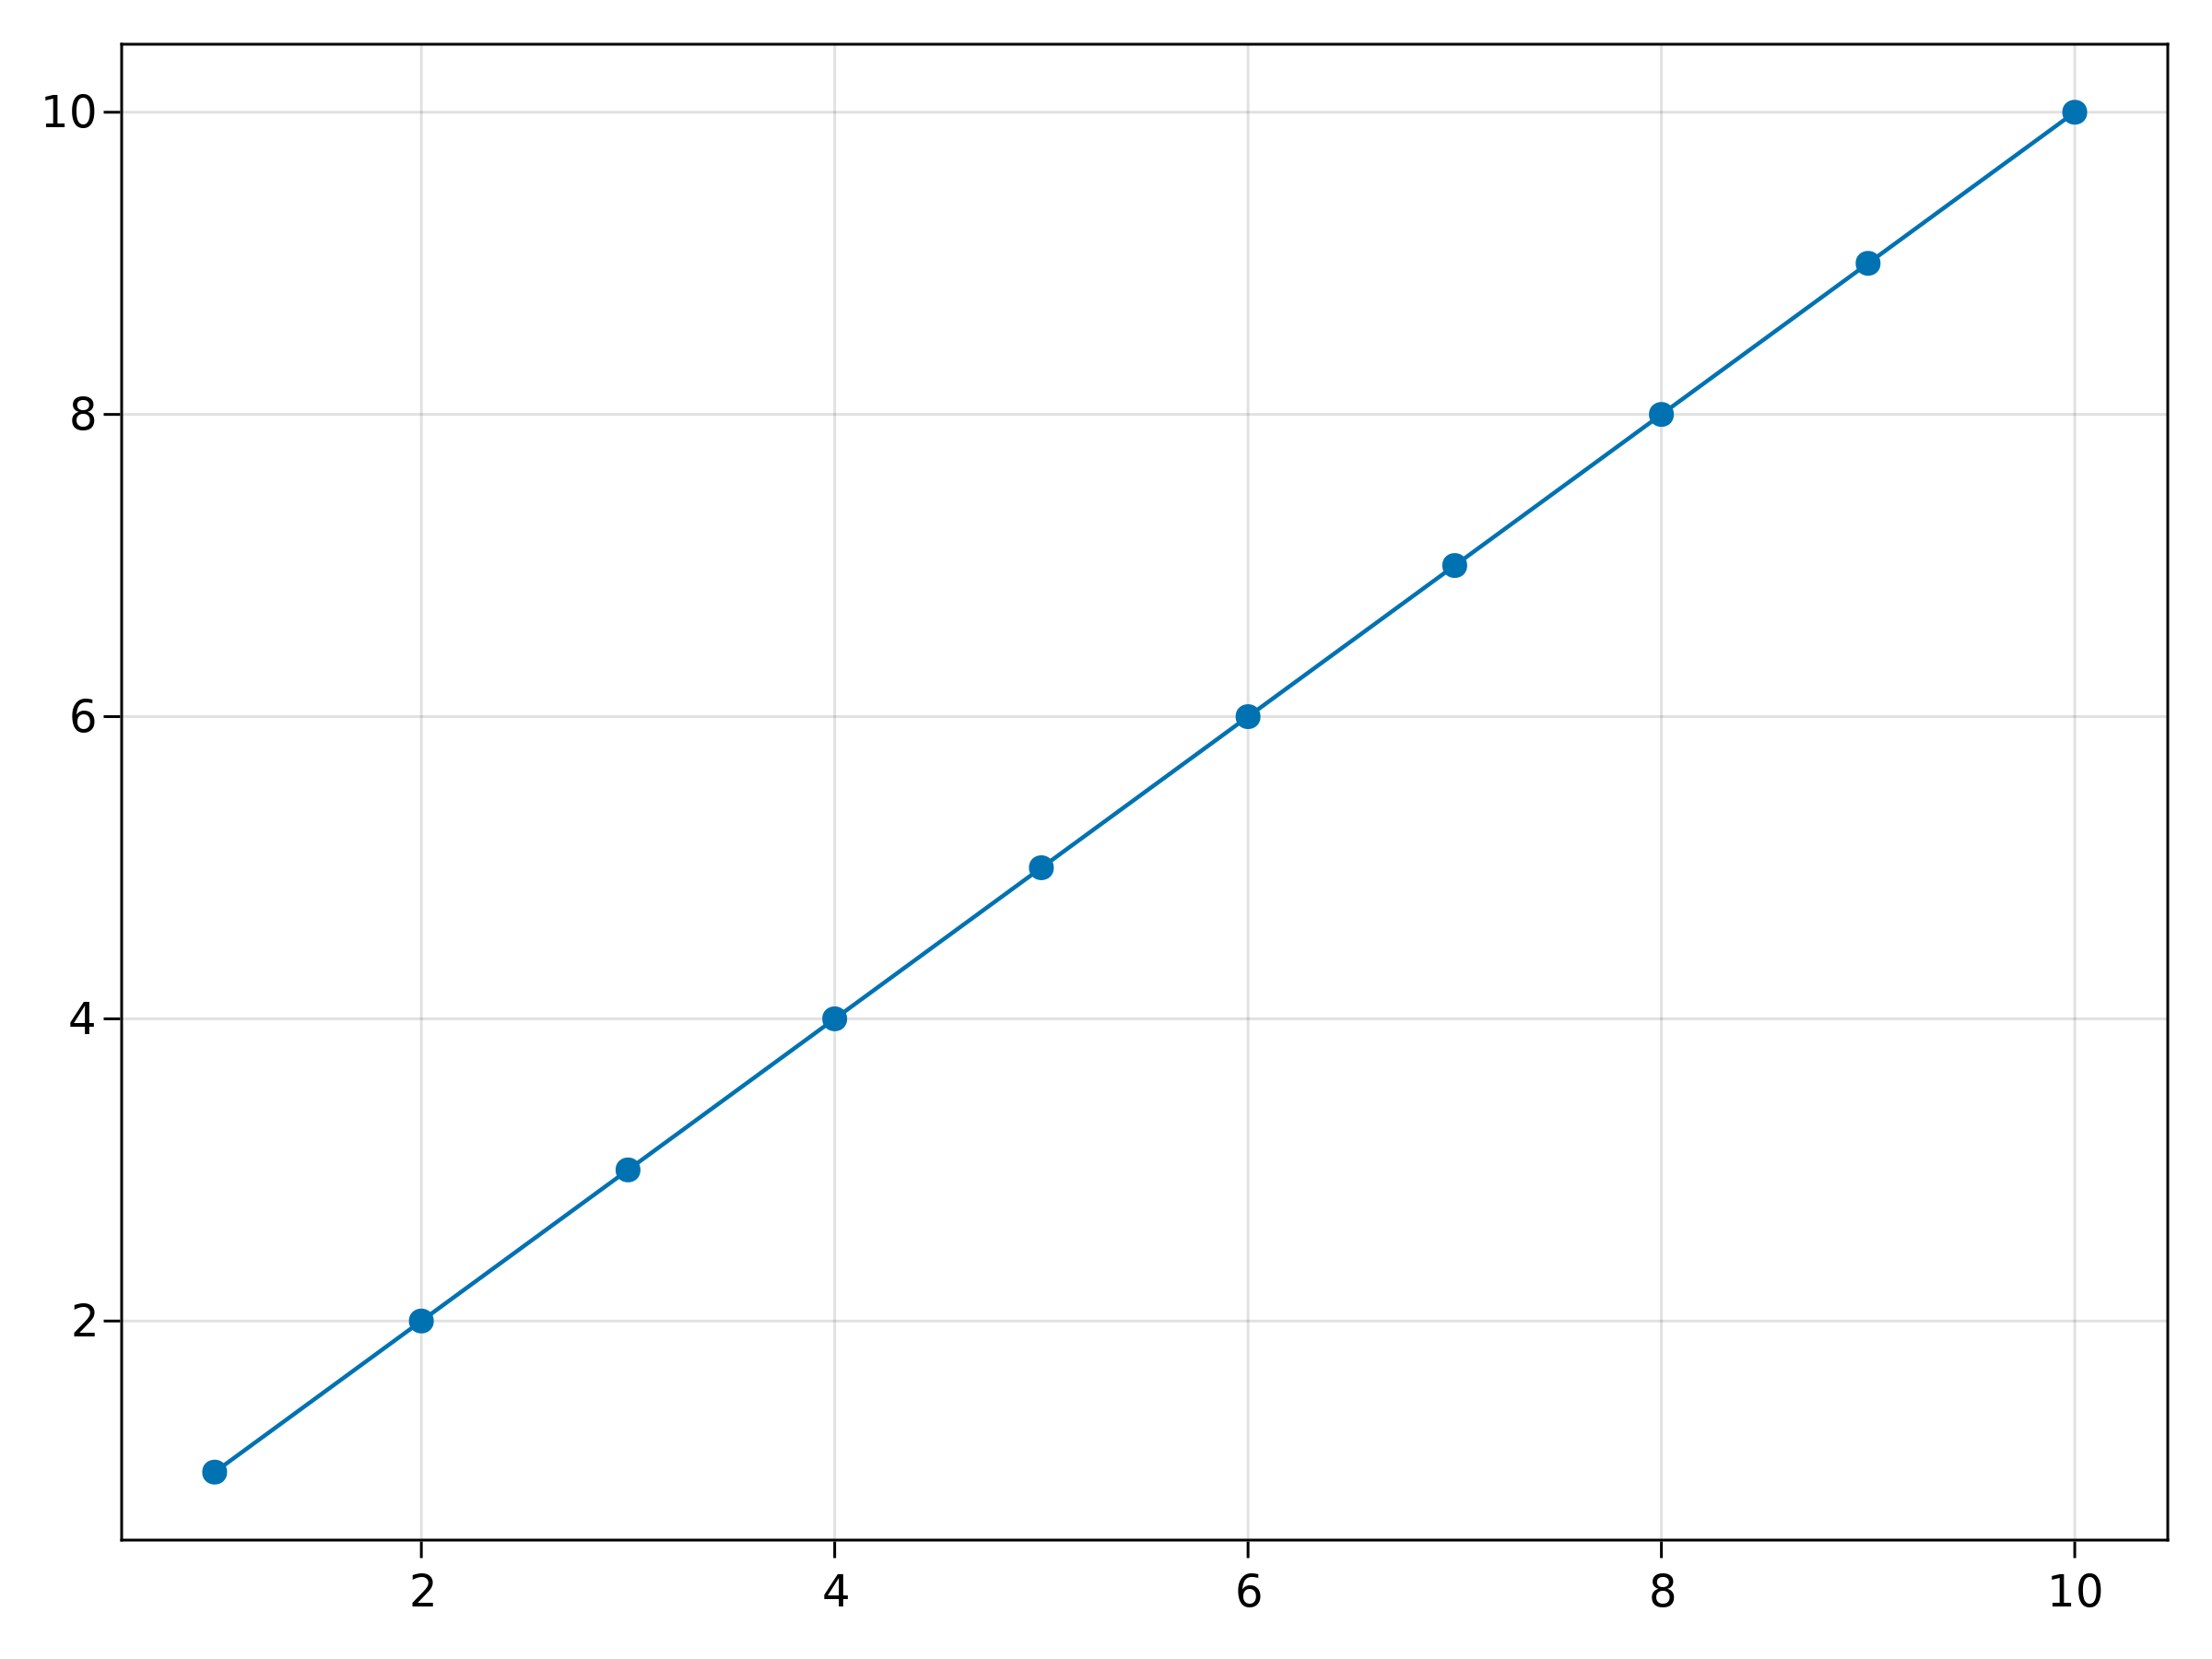
\includegraphics[width=0.6\textwidth,height=\textheight]{_build/im/firstplot.png}
\caption{First plot.}\label{fig:firstplot}
}
\end{figure}

Note that the previous plot is the default output, which we probably
need to tweak by using axis names and labels.

Also note that every plotting function like
\passthrough{\lstinline!scatterlines!} creates and returns a new
\passthrough{\lstinline!Figure!}, \passthrough{\lstinline!Axis!} and
\passthrough{\lstinline!plot!} object in a collection called
\passthrough{\lstinline!FigureAxisPlot!}. These are known as the
\passthrough{\lstinline!non-mutating!} methods. On the other hand, the
\passthrough{\lstinline!mutating!} methods
(e.g.~\passthrough{\lstinline"scatterlines!"}, note the
\passthrough{\lstinline"!"}) just return a plot object which can be
appended into a given \passthrough{\lstinline!axis!} or the
\passthrough{\lstinline!current\_figure()!}.

The next question that one might have is: how do I change the color or
the marker type? This can be done via
\passthrough{\lstinline!attributes!}, which we do in the next section.

\hypertarget{sec:datavisMakie_attributes}{%
\section{Attributes}\label{sec:datavisMakie_attributes}}

A custom plot can be created by using
\passthrough{\lstinline!attributes!}. The attributes can be set through
keyword arguments. A list of \passthrough{\lstinline!attributes!} for
every plotting object can be viewed via:

\begin{lstlisting}[language=Julia]
fig, ax, pltobj = scatterlines(1:10)
pltobj.attributes
\end{lstlisting}

\begin{lstlisting}[language=Output]
Attributes with 15 entries:
  color => RGBA{Float32}(0.0,0.447059,0.698039,1.0)
  colormap => viridis
  colorrange => Automatic()
  cycle => [:color]
  inspectable => true
  linestyle => nothing
  linewidth => 1.5
  marker => Circle
  markercolor => Automatic()
  markercolormap => viridis
  markercolorrange => Automatic()
  markersize => 9
  model => Float32[1.0 0.0 0.0 0.0; 0.0 1.0 0.0 0.0; 0.0 0.0 1.0 0.0; 0.0 0.0 0.0 1.0]
  strokecolor => black
  strokewidth => 0
\end{lstlisting}

Or as a \passthrough{\lstinline!Dict!} calling
\passthrough{\lstinline!pltobj.attributes.attributes!}.

Asking for help in the \passthrough{\lstinline!REPL!} as
\passthrough{\lstinline!?lines!} or
\passthrough{\lstinline!help(lines)!} for any given plotting function
will show you their corresponding attributes plus a short description on
how to use that specific function. For example, for
\passthrough{\lstinline!lines!}:

\begin{lstlisting}[language=Julia]
help(lines)
\end{lstlisting}

\begin{lstlisting}[language=Output]
  lines(positions)
  lines(x, y)
  lines(x, y, z)

  Creates a connected line plot for each element in (x, y, z), (x, y) or
  positions.

  │ Tip
  │
  │  You can separate segments by inserting NaNs.

  lines has the following function signatures:

    (Vector, Vector)
    (Vector, Vector, Vector)
    (Matrix)

  Available attributes for Lines are:

    color
    colormap
    colorrange
    cycle
    depth_shift
    diffuse
    inspectable
    linestyle
    linewidth
    nan_color
    overdraw
    shininess
    space
    specular
    ssao
    transparency
    visible
\end{lstlisting}

Not only the plot objects have attributes, also the
\passthrough{\lstinline!Axis!} and \passthrough{\lstinline!Figure!}
objects do. For example, for Figure, we have
\passthrough{\lstinline!backgroundcolor!},
\passthrough{\lstinline!resolution!}, \passthrough{\lstinline!font!} and
\passthrough{\lstinline!fontsize!} as well as the
\passthrough{\lstinline!figure\_padding!} which changes the amount of
space around the figure content, see the grey area in
Figure~\ref{fig:custom_plot}. It can take one number for all sides, or a
tuple of four numbers for left, right, bottom and top.

\passthrough{\lstinline!Axis!} has a lot more, some of them are
\passthrough{\lstinline!backgroundcolor!},
\passthrough{\lstinline!xgridcolor!} and
\passthrough{\lstinline!title!}. For a full list just type
\passthrough{\lstinline!help(Axis)!}.

Hence, for our next plot we will call several attributes at once as
follows:

\begin{lstlisting}[language=Julia]
lines(1:10, (1:10).^2; color=:black, linewidth=2, linestyle=:dash,
    figure=(; figure_padding=5, resolution=(600, 400), font="sans",
        backgroundcolor=:grey90, fontsize=16),
    axis=(; xlabel="x", ylabel="x²", title="title",
        xgridstyle=:dash, ygridstyle=:dash))
current_figure()
\end{lstlisting}

\begin{figure}
\hypertarget{fig:custom_plot}{%
\centering
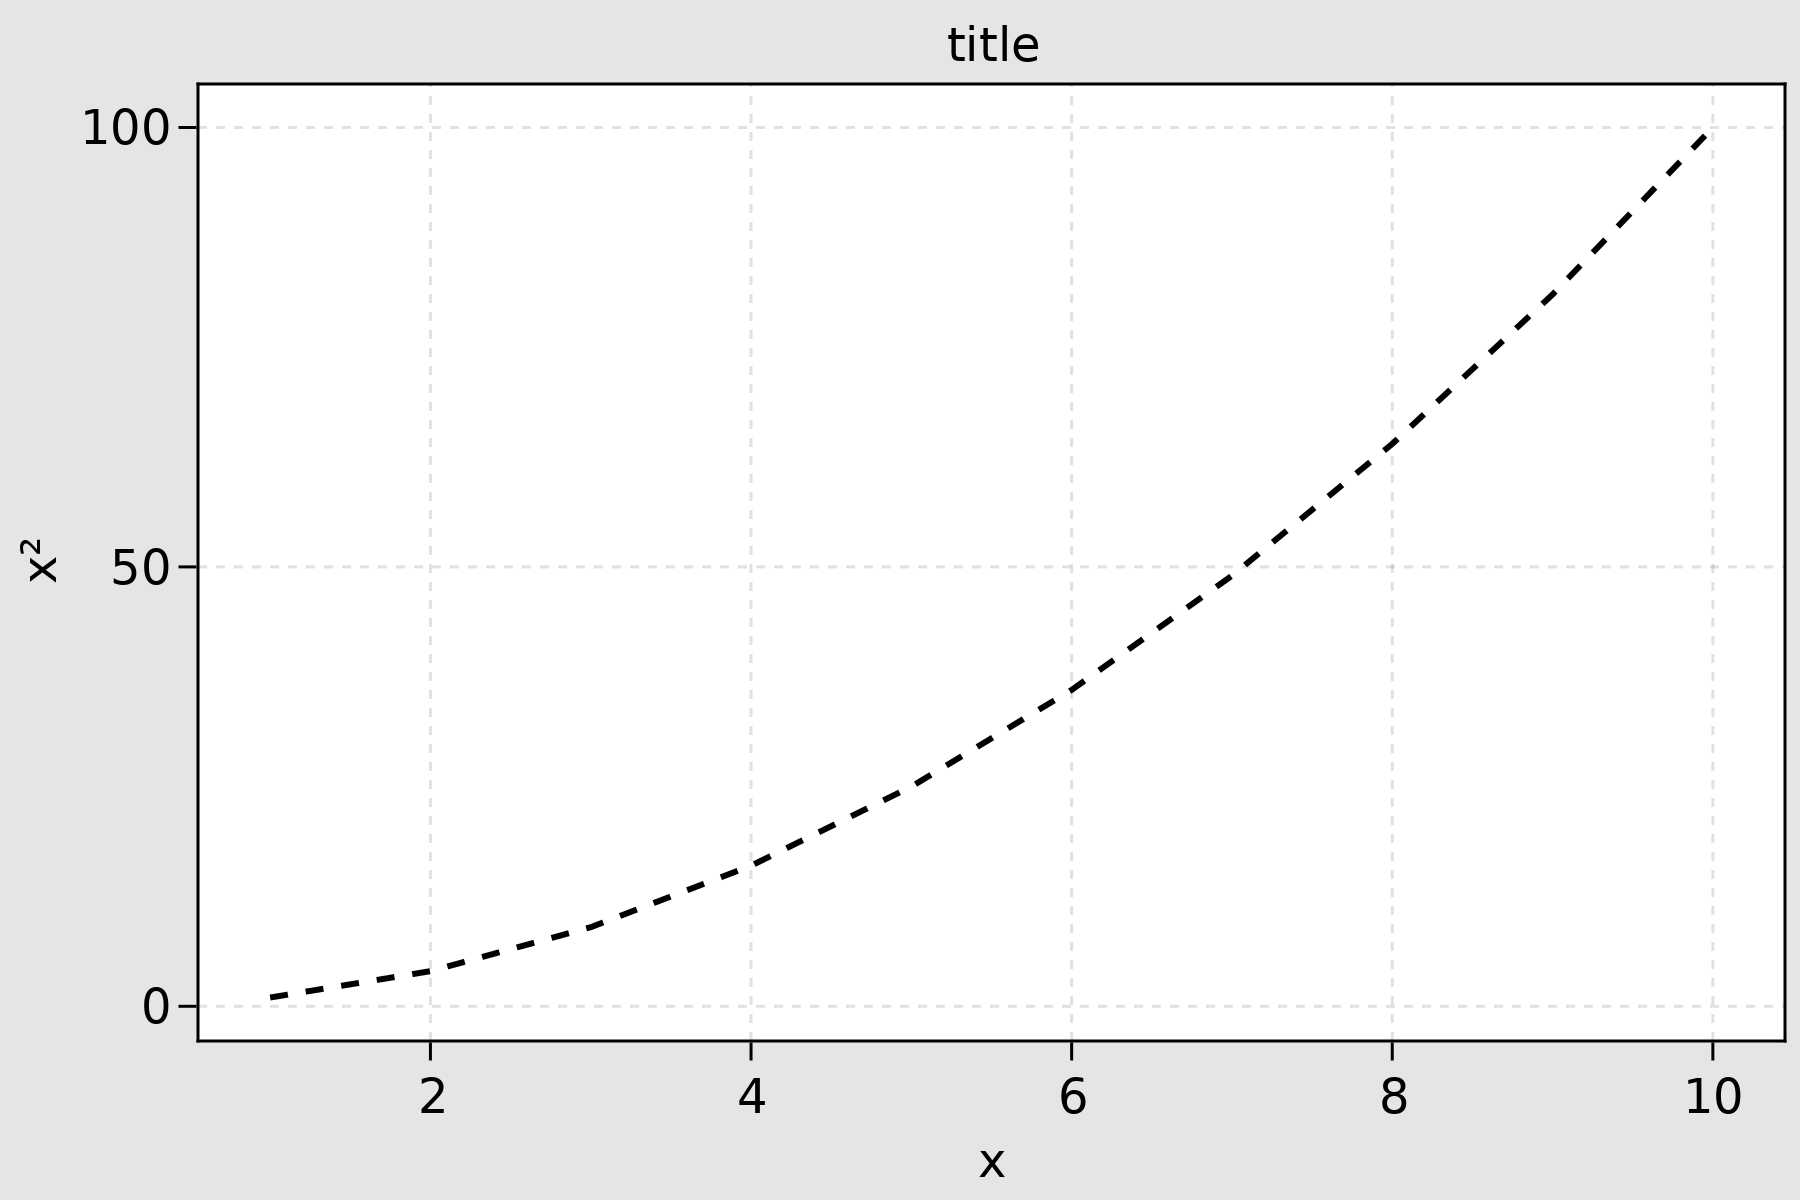
\includegraphics[width=0.6\textwidth,height=\textheight]{_build/im/custom_plot.png}
\caption{Custom plot.}\label{fig:custom_plot}
}
\end{figure}

This example has already most of the attributes that most users will
normally use. Probably, a \passthrough{\lstinline!legend!} will also be
good to have. Which for more than one function will make more sense. So,
let's \passthrough{\lstinline!append!} another mutation
\passthrough{\lstinline!plot!} object and add the corresponding legends
by calling \passthrough{\lstinline!axislegend!}. This will collect all
the \passthrough{\lstinline!labels!} you might have passed to your
plotting functions and by default will be located in the right top
position. For a different one, the
\passthrough{\lstinline!position=:ct!} argument is called, where
\passthrough{\lstinline!:ct!} means let's put our label in the
\passthrough{\lstinline!center!} and at the
\passthrough{\lstinline!top!}, see Figure
Figure~\ref{fig:custom_plot_leg}:

\begin{lstlisting}[language=Julia]
lines(1:10, (1:10).^2; label="x²", linewidth=2, linestyle=nothing,
    figure=(; figure_padding=5, resolution=(600, 400), font="sans",
        backgroundcolor=:grey90, fontsize=16),
    axis=(; xlabel="x", title="title", xgridstyle=:dash,
        ygridstyle=:dash))
scatterlines!(1:10, (10:-1:1).^2; label="Reverse(x)²")
axislegend("legend"; position=:ct)
current_figure()
\end{lstlisting}

\begin{figure}
\hypertarget{fig:custom_plot_leg}{%
\centering
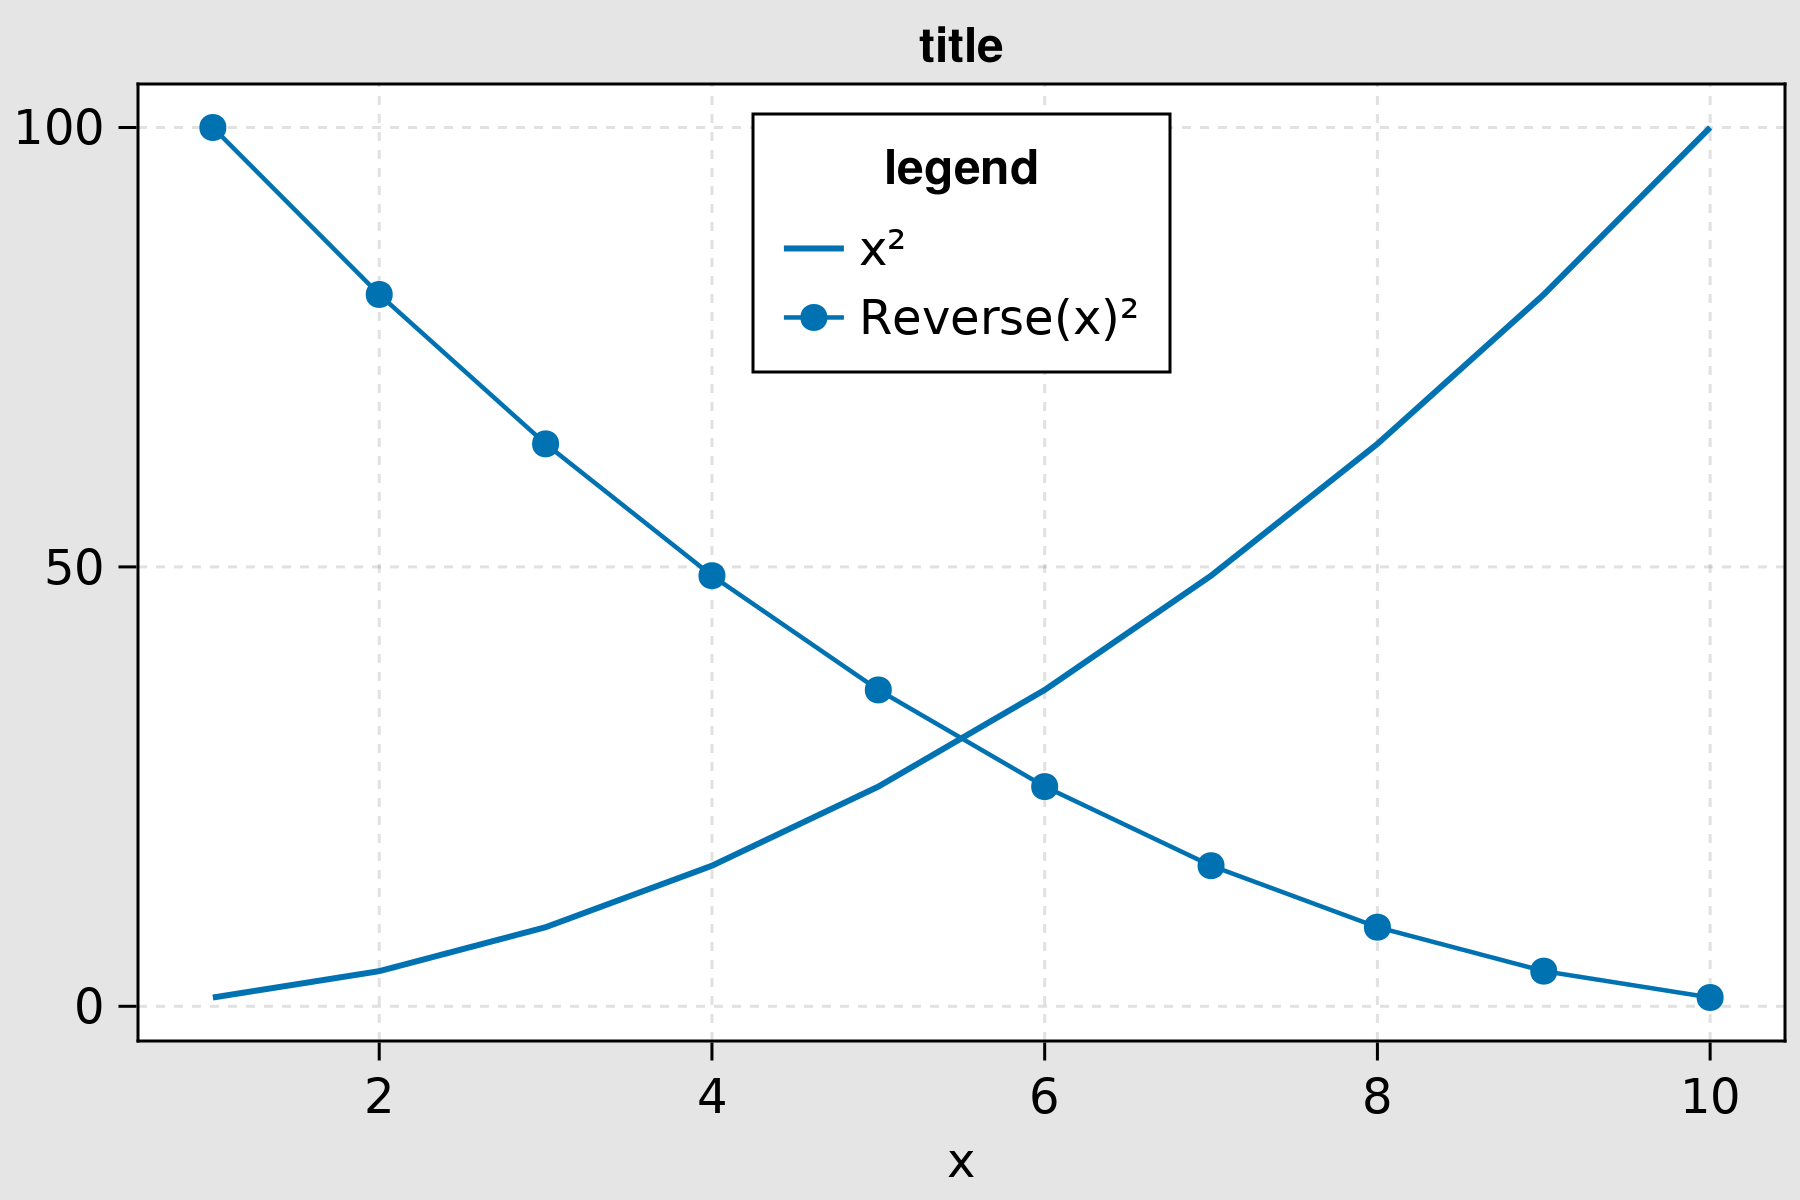
\includegraphics[width=0.6\textwidth,height=\textheight]{_build/im/custom_plot_leg.png}
\caption{Custom plot legend.}\label{fig:custom_plot_leg}
}
\end{figure}

Other positions are also available by combining \emph{left(l),
center(c), right(r)} and \emph{bottom(b), center(c), top(t)}. For
instance, for left top, use \passthrough{\lstinline!:lt!}.

However, having to write this much code just for two lines is
cumbersome. So, if you plan on doing a lot of plots with the same
general aesthetics, then setting a theme will be better. We can do this
with \passthrough{\lstinline"set\_theme!()"} as the following example
illustrates.

Plotting the previous figure should take the new default settings
defined by \passthrough{\lstinline"set\_theme!(kwargs)"}:

\begin{lstlisting}[language=Julia]
set_theme!(; resolution=(600, 400),
    backgroundcolor=(:orange, 0.5), fontsize=16, font="sans",
    Axis=(backgroundcolor=:grey90, xgridstyle=:dash, ygridstyle=:dash),
    Legend=(bgcolor=(:red, 0.2), framecolor=:dodgerblue))
lines(1:10, (1:10).^2; label="x²", linewidth=2, linestyle=nothing,
    axis=(; xlabel="x", title="title"))
scatterlines!(1:10, (10:-1:1).^2; label="Reverse(x)²")
axislegend("legend"; position=:ct)
current_figure()
set_theme!()
\end{lstlisting}

\begin{figure}
\hypertarget{fig:setTheme}{%
\centering
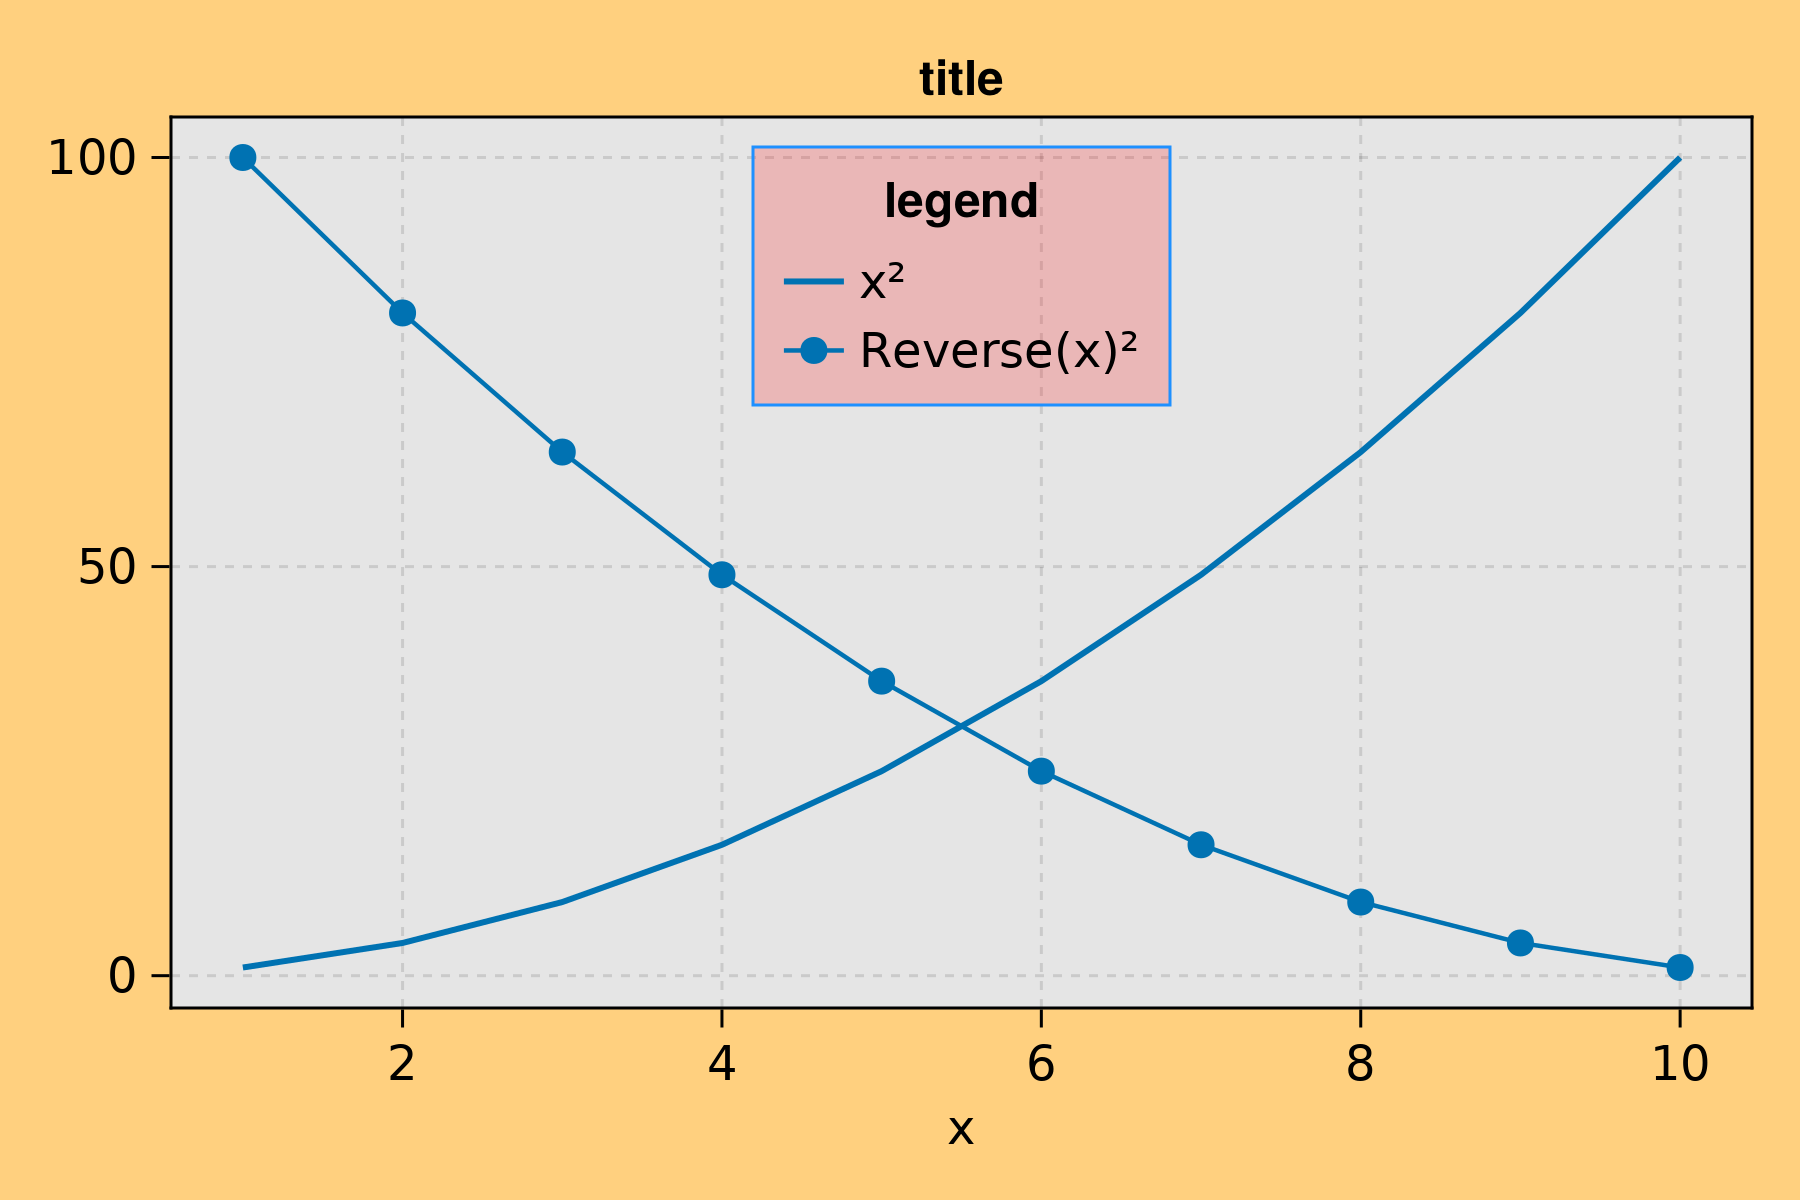
\includegraphics[width=0.6\textwidth,height=\textheight]{_build/im/setTheme.png}
\caption{Set theme example.}\label{fig:setTheme}
}
\end{figure}

Note that the last line is \passthrough{\lstinline"set\_theme!()"},
which will reset to the default settings of Makie. For more on
\passthrough{\lstinline!themes!} please go to Section~\ref{sec:themes}.

Before moving on into the next section, it's worthwhile to see an
example where an \passthrough{\lstinline!array!} of attributes is passed
at once to a plotting function. For this example, we will use the
\passthrough{\lstinline!scatter!} plotting function to do a bubble plot.

The data for this could be an \passthrough{\lstinline!array!} with 100
rows and 3 columns, which we generated at random from a normal
distribution. Here, the first column could be the positions in the
\passthrough{\lstinline!x!} axis, the second one the positions in
\passthrough{\lstinline!y!} and the third one an intrinsic associated
value for each point. The latter could be represented in a plot by a
different \passthrough{\lstinline!color!} or with a different marker
size. In a bubble plot we can do both.

\begin{lstlisting}[language=Julia]
using Random: seed!
seed!(28)
xyvals = randn(100, 3)
xyvals[1:5, :]
\end{lstlisting}

\begin{lstlisting}[language=Output]
5×3 Matrix{Float64}:
  0.550992   1.27614    -0.659886
 -1.06587   -0.0287242   0.175126
 -0.721591  -1.84423     0.121052
  0.801169   0.862781   -0.221599
 -0.340826   0.0589894  -1.76359
\end{lstlisting}

Next, the corresponding plot can be seen in Figure~\ref{fig:bubble}:

\begin{lstlisting}[language=Julia]
fig, ax, pltobj = scatter(xyvals[:, 1], xyvals[:, 2]; color=xyvals[:, 3],
    label="Bubbles", colormap=:plasma, markersize=15 * abs.(xyvals[:, 3]),
    figure=(; resolution=(600, 400)), axis=(; aspect=DataAspect()))
limits!(-3, 3, -3, 3)
Legend(fig[1, 2], ax, valign=:top)
Colorbar(fig[1, 2], pltobj, height=Relative(3 / 4))
fig
\end{lstlisting}

\begin{figure}
\hypertarget{fig:bubble}{%
\centering
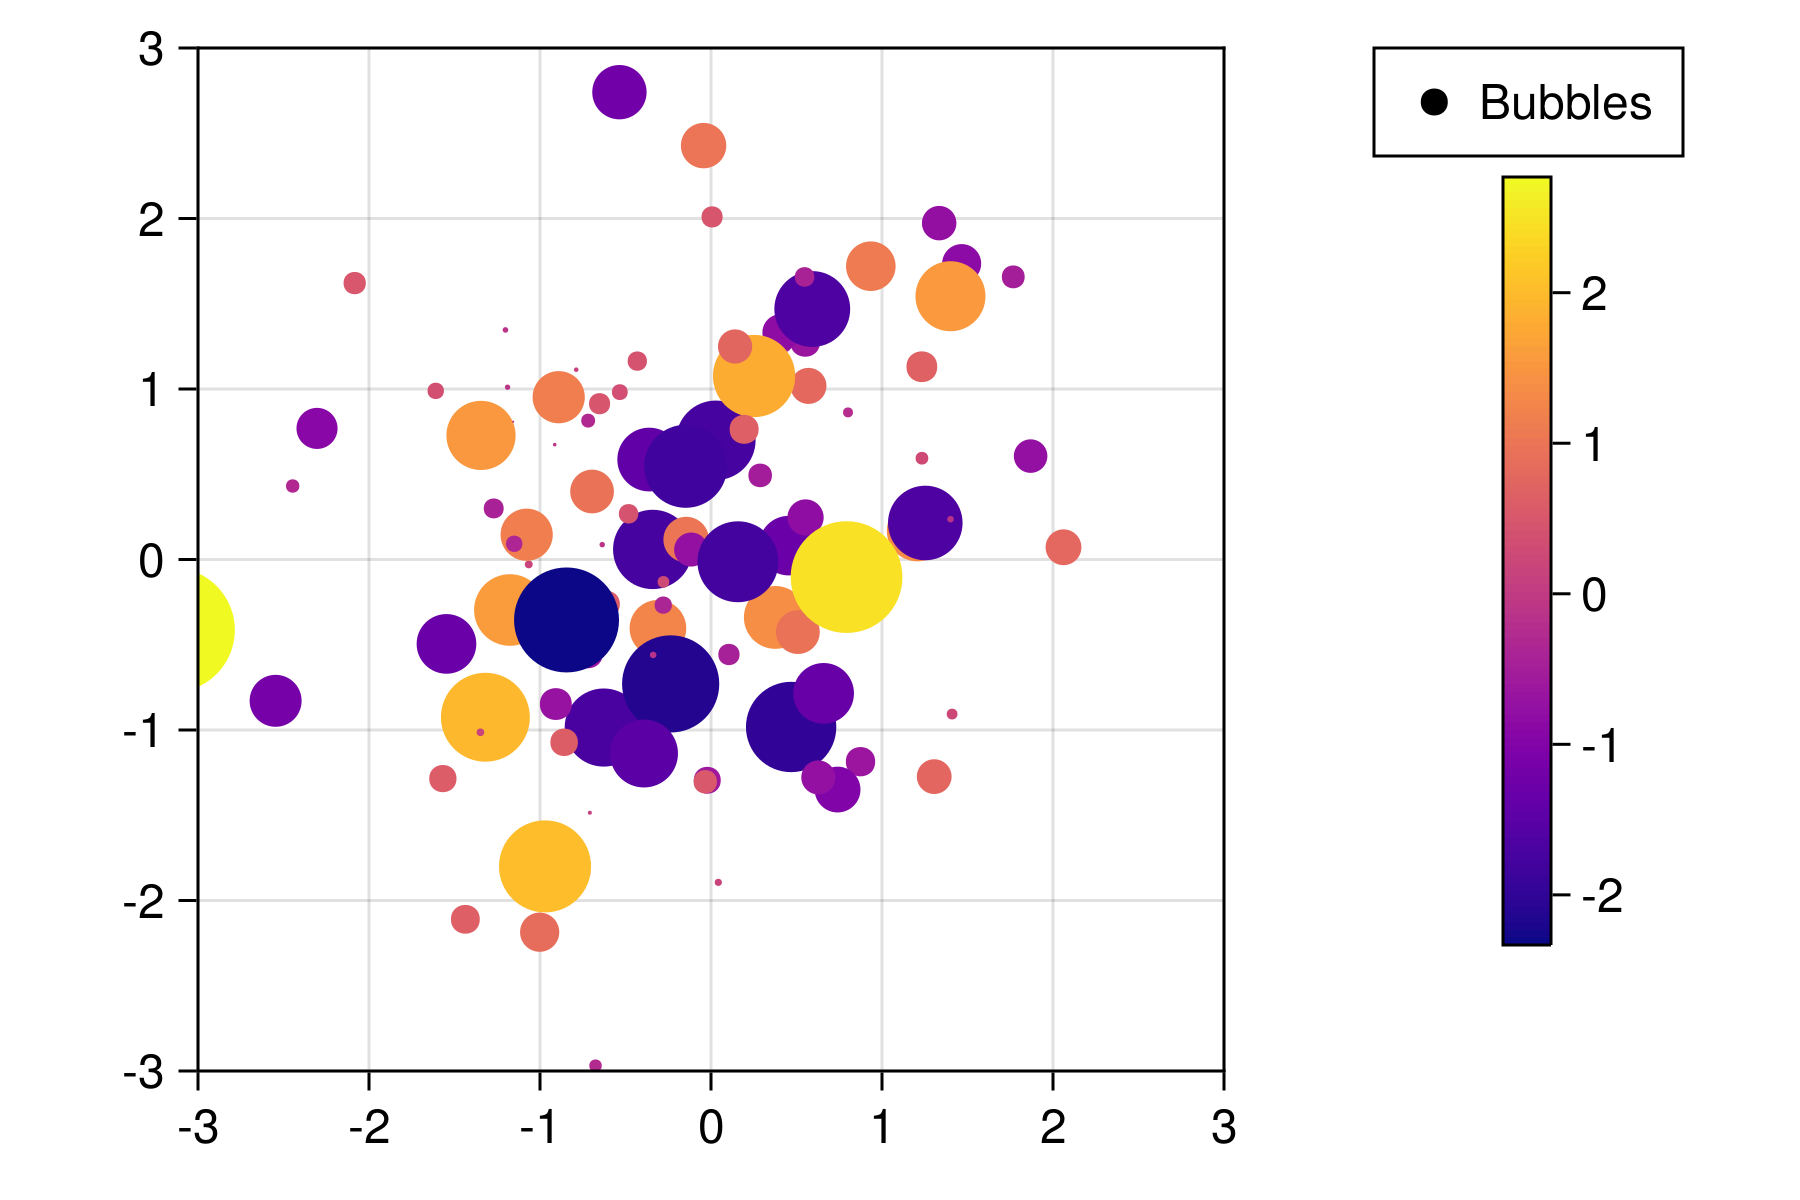
\includegraphics[width=0.6\textwidth,height=\textheight]{_build/im/bubble.png}
\caption{Bubble plot.}\label{fig:bubble}
}
\end{figure}

where we have decomposed the tuple
\passthrough{\lstinline!FigureAxisPlot!} into
\passthrough{\lstinline!fig, ax, pltobj!}, in order to be able to add a
\passthrough{\lstinline!Legend!} and \passthrough{\lstinline!Colorbar!}
outside of the plotted object. We will discuss layout options in more
detail in Section~\ref{sec:makie_layouts}.

We have done some basic but still interesting examples to show how to
use \passthrough{\lstinline!Makie.jl!} and by now you might be
wondering: what else can we do? What are all the possible plotting
functions available in \passthrough{\lstinline!Makie.jl!}? To answer
this question, a \emph{cheat sheet} is shown in
Figure~\ref{fig:cheat_sheet_cairomakie}. These work especially well with
\passthrough{\lstinline!CairoMakie.jl!} backend.

\begin{figure}
\hypertarget{fig:cheat_sheet_cairomakie}{%
\centering
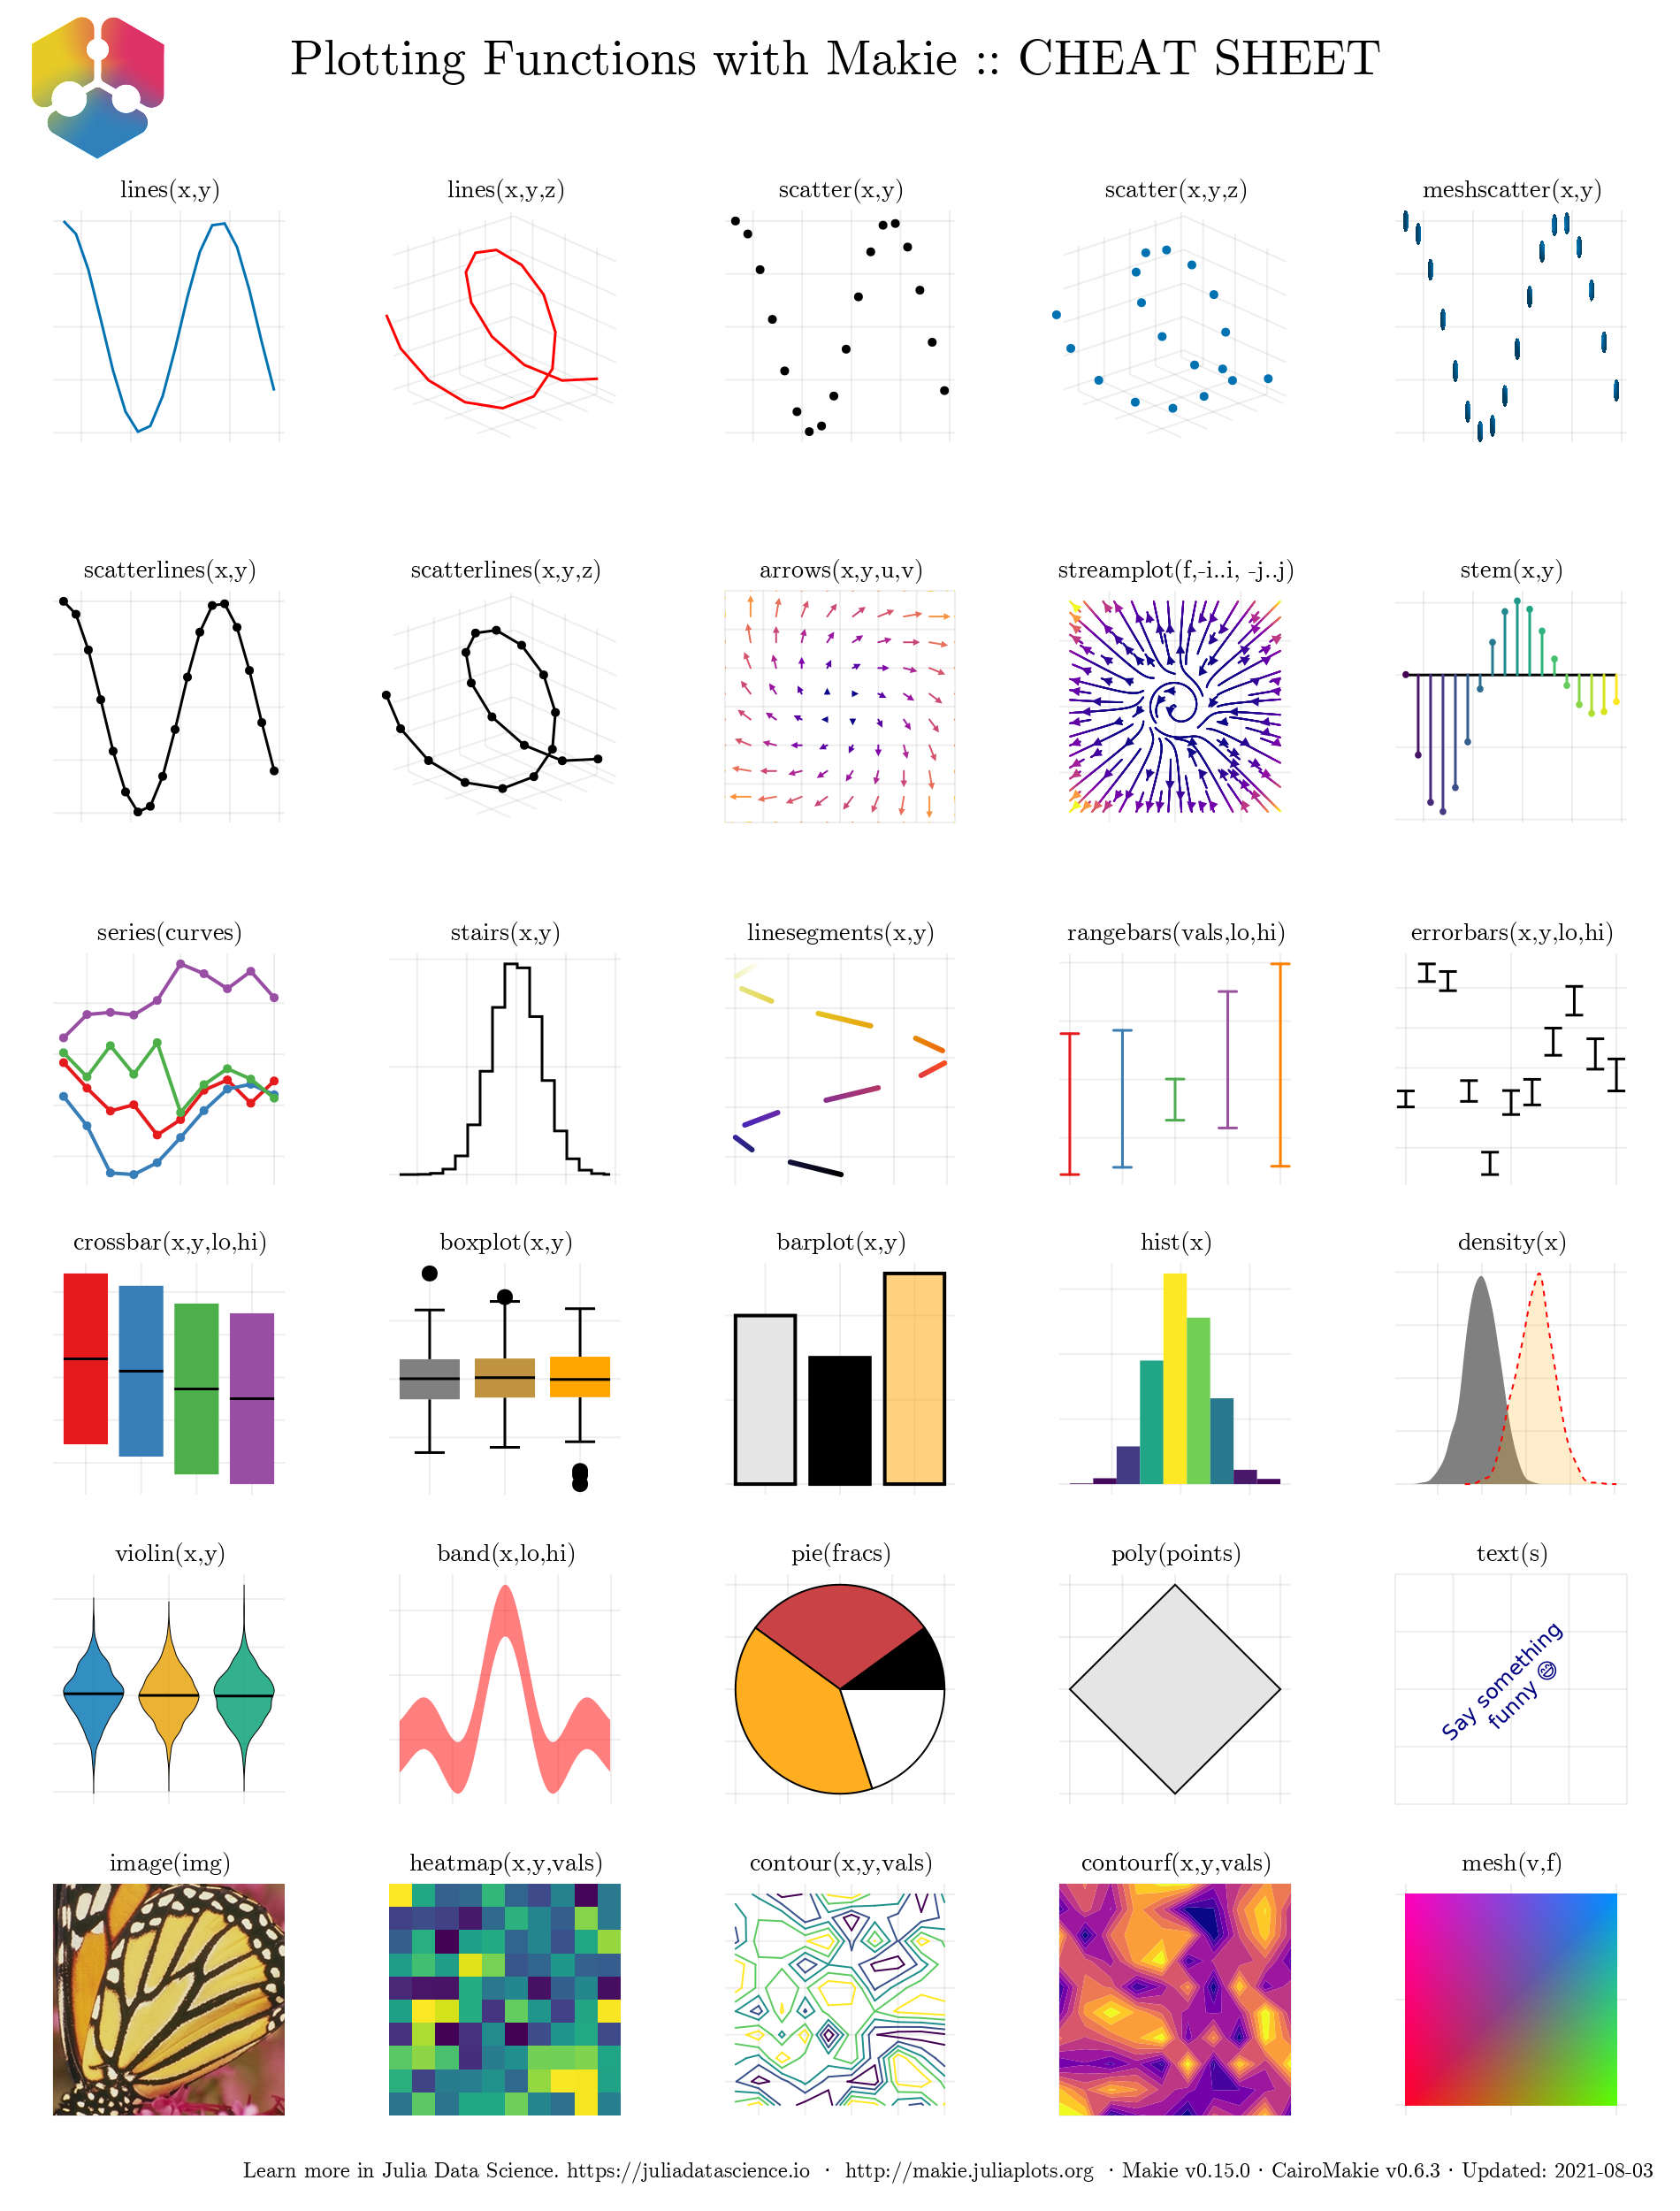
\includegraphics{images/makiePlottingFunctionsHide.png}
\caption{Plotting functions: Cheat Sheet. Output given by
Cairomakie.}\label{fig:cheat_sheet_cairomakie}
}
\end{figure}

For completeness, in Figure~\ref{fig:cheat_sheet_glmakie}, we show the
corresponding functions \emph{cheat sheet} for
\passthrough{\lstinline!GLMakie.jl!}, which supports mostly 3D plots.
Those will be explained in detail in Section~\ref{sec:glmakie}.

\begin{figure}
\hypertarget{fig:cheat_sheet_glmakie}{%
\centering
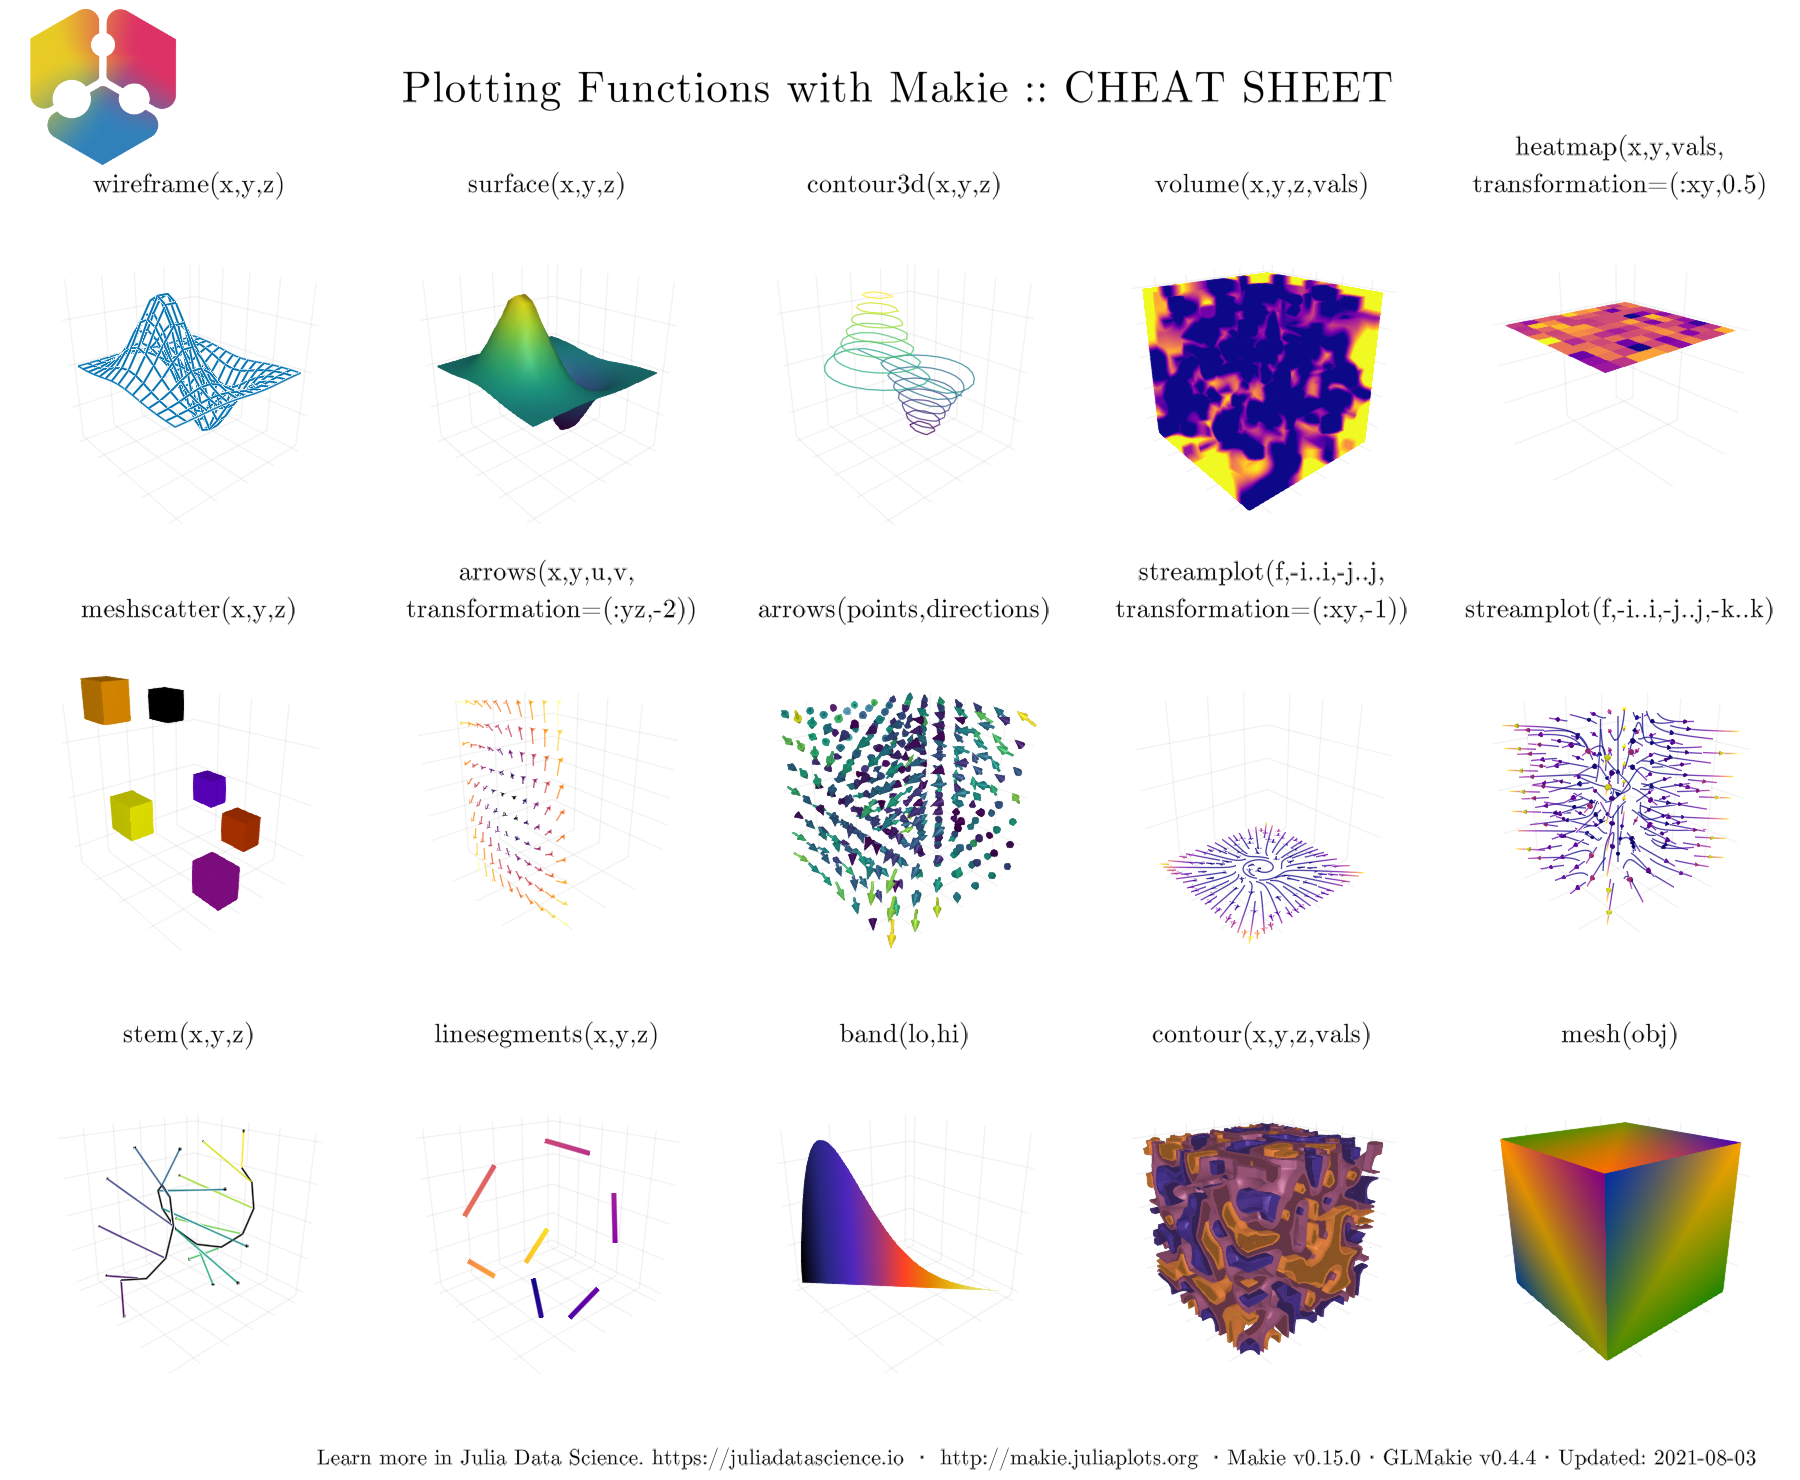
\includegraphics{images/GLMakiePlottingFunctionsHide.png}
\caption{Plotting functions: Cheat Sheet. Output given by
GLMakie.}\label{fig:cheat_sheet_glmakie}
}
\end{figure}

Now, that we have an idea of all the things we can do, let's go back and
continue with the basics. It's time to learn how to change the general
appearance of our plots.

\hypertarget{sec:themes}{%
\section{Themes}\label{sec:themes}}

There are several ways to affect the general appearance of your plots.
Either, you could use a
\href{http://makie.juliaplots.org/stable/documentation/theming/predefined_themes/index.html}{predefined
theme} or your own custom theme. For example, use the predefined dark
theme via
\passthrough{\lstinline!with\_theme(your\_plot\_function, theme\_dark())!}.
Or, build your own with \passthrough{\lstinline!Theme(kwargs)!} or even
update the one that is active with
\passthrough{\lstinline"update\_theme!(kwargs)"}.

You can also do \passthrough{\lstinline"set\_theme!(theme; kwargs...)"}
to change the current default theme to \passthrough{\lstinline!theme!}
and override or add attributes given by
\passthrough{\lstinline!kwargs!}. If you do this and want to reset all
previous settings just do \passthrough{\lstinline"set\_theme!()"} with
no arguments. See the following examples, where we had prepared a test
plotting function with different characteristics, such that most
attributes for each theme can be appreciated.

\begin{lstlisting}[language=Julia]
using Random: seed!
seed!(123)
y = cumsum(randn(6, 6), dims=2)
\end{lstlisting}

\begin{lstlisting}[language=Output]
6×6 Matrix{Float64}:
  0.808288   0.386519   0.355371   0.0365011  -0.0911358   1.8115
 -1.12207   -2.47766   -2.16183   -2.49928    -2.02981    -1.37017
 -1.10464   -1.03518   -3.19756   -1.18944    -2.71633    -3.80455
 -0.416993  -0.534315  -1.42439   -0.659362   -0.0592298   0.644529
  0.287588   1.50687    2.36111    2.54137     0.48751     0.630836
  0.229819   0.522733   0.864515   2.89343     2.06537     2.21375
\end{lstlisting}

A matrix of size \passthrough{\lstinline!(20, 20)!} with random entries,
so that we can plot a heatmap. The range in \(x\) and \(y\) is also
specified.

\begin{lstlisting}[language=Julia]
using Random: seed!
seed!(13)
xv = yv = LinRange(-3, 0.5, 20)
matrix = randn(20, 20)
matrix[1:6, 1:6] # first 6 rows and columns
\end{lstlisting}

\begin{lstlisting}[language=Output]
6×6 Matrix{Float64}:
 -0.271257   0.894952   0.728865  -0.293849   -0.449277   -0.0948871
 -0.193033  -0.421286  -0.455905  -0.0576092  -0.756621   -1.47419
 -0.123177   0.762254   0.773921  -0.38526    -0.0659695  -0.599284
 -1.47327    0.770122   1.20725    0.257913    0.111979    0.875439
 -1.82913   -0.603888   0.164083  -0.118504    1.46723     0.0948876
  1.09769    0.178207   0.110243  -0.543203    0.592245    0.328993
\end{lstlisting}

Hence, our plotting function looks like follows:

\begin{lstlisting}[language=Julia]
function demo_themes(y, xv, yv, matrix)
    fig, _ = series(y; labels=["$i" for i = 1:6], markersize=10,
        color=:Set1, figure=(; resolution=(600, 300)),
        axis=(; xlabel="time (s)", ylabel="Amplitude",
            title="Measurements"))
    hmap = heatmap!(xv, yv, matrix; colormap=:plasma)
    limits!(-3.1, 8.5, -6, 5.1)
    axislegend("legend"; merge=true)
    Colorbar(fig[1, 2], hmap)
    fig
end
\end{lstlisting}

Note that the \passthrough{\lstinline!series!} function has been used to
plot several lines and scatters at once with their corresponding labels.
And since we don't need the axis neither the plotted object we throw
them away with the syntax *\_*. Also, a heatmap with their
\passthrough{\lstinline!Colorbar!} has been included. Currently, there
are two dark themes, one called \passthrough{\lstinline!theme\_dark()!}
and the other one \passthrough{\lstinline!theme\_black()!}, see Figures.

\begin{lstlisting}[language=Julia]
with_theme(theme_dark()) do
    demo_themes(y, xv, yv, matrix)
end
with_theme(theme_black()) do
    demo_themes(y, xv, yv, matrix)
end
\end{lstlisting}

\begin{figure}
\hypertarget{fig:theme_dark}{%
\centering
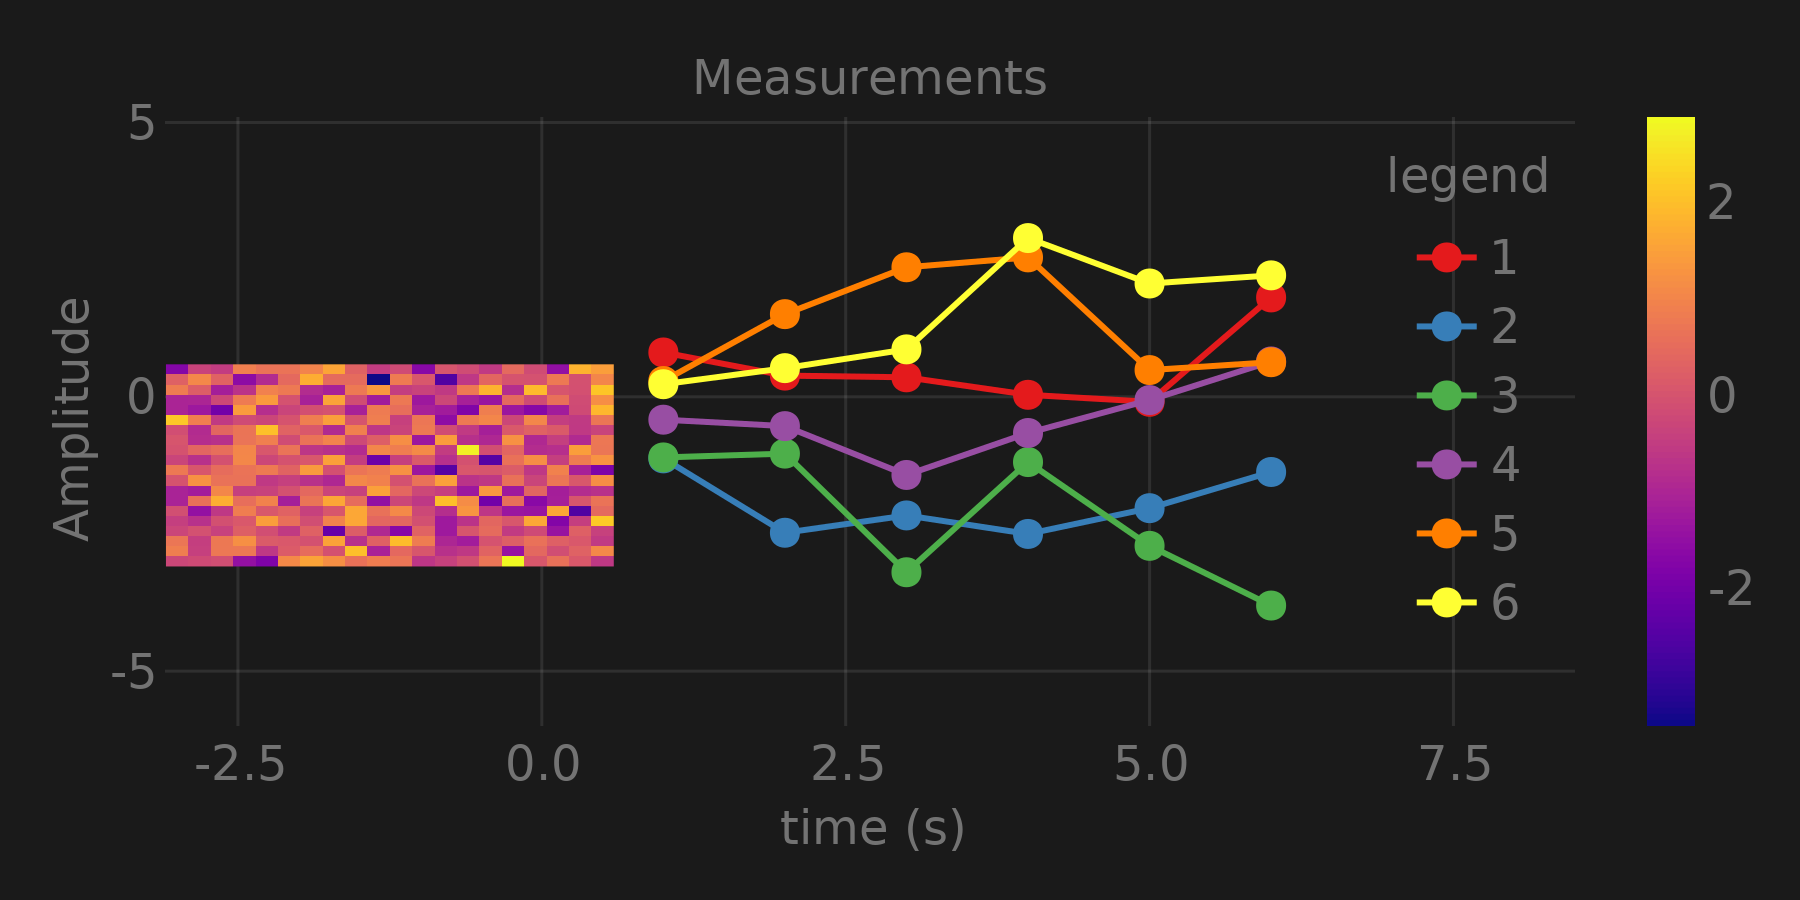
\includegraphics[width=0.6\textwidth,height=\textheight]{_build/im/theme_dark.png}
\caption{Theme dark.}\label{fig:theme_dark}
}
\end{figure}

\begin{figure}
\hypertarget{fig:theme_black}{%
\centering
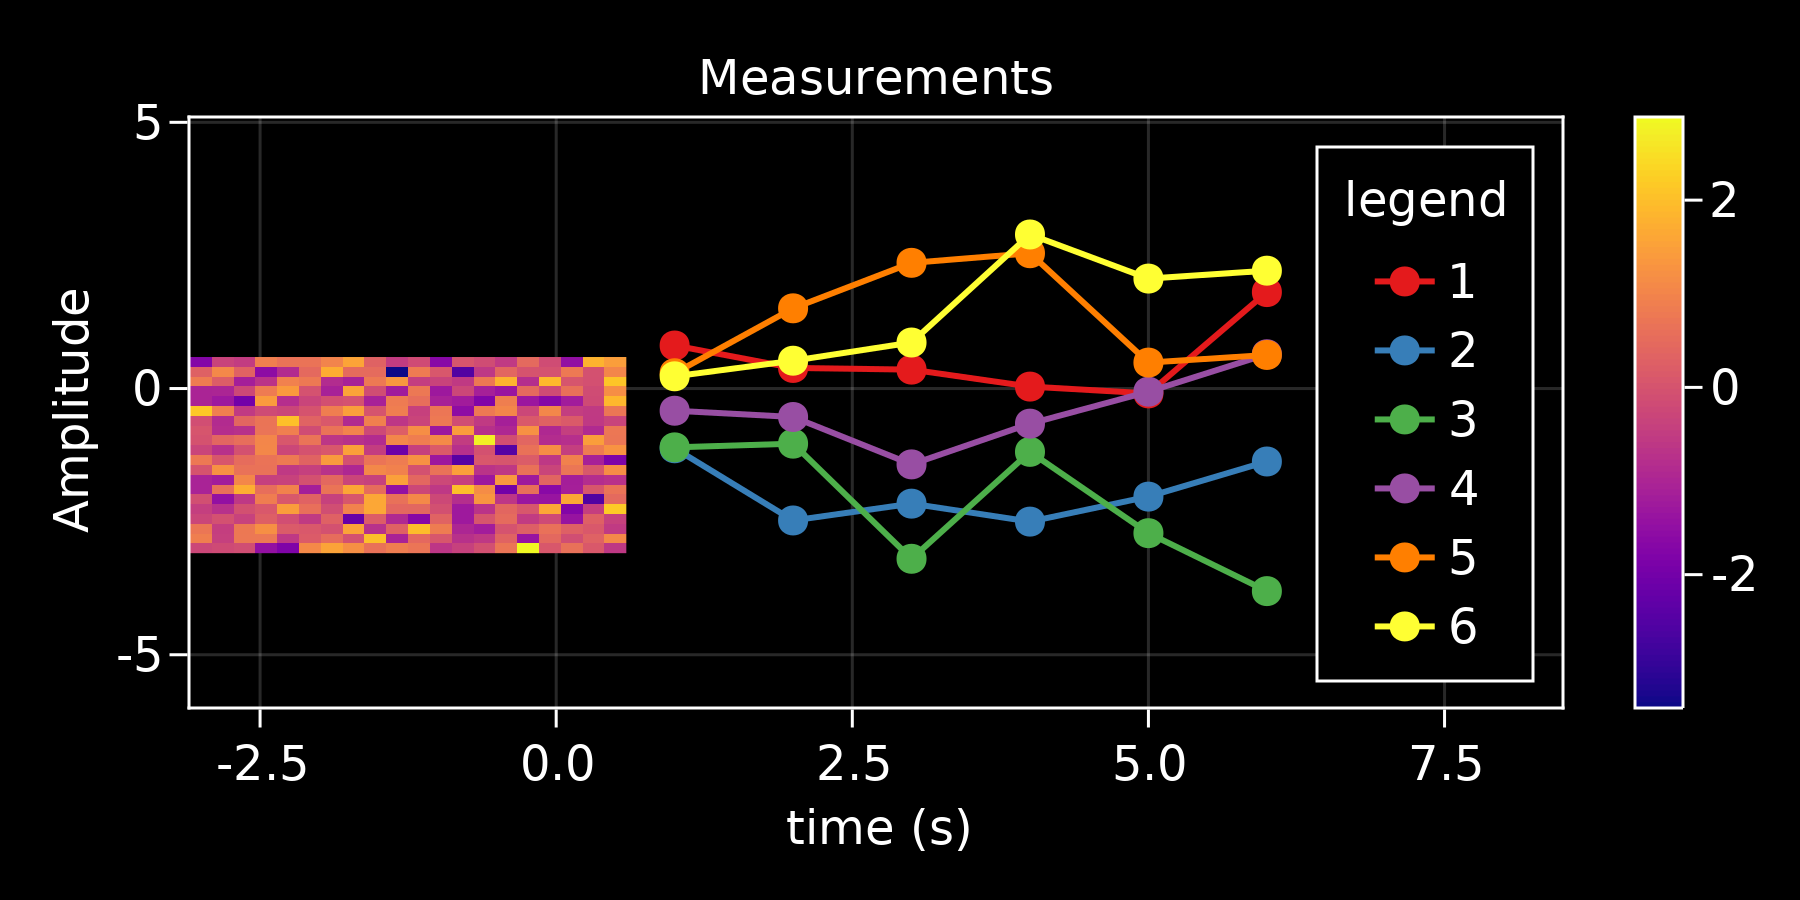
\includegraphics[width=0.6\textwidth,height=\textheight]{_build/im/theme_black.png}
\caption{Theme black.}\label{fig:theme_black}
}
\end{figure}

And three more white-ish themes called,
\passthrough{\lstinline!theme\_ggplot2()!},
\passthrough{\lstinline!theme\_minimal()!} and
\passthrough{\lstinline!theme\_light()!}. Useful for more standard
publication type plots.

\begin{lstlisting}[language=Julia]
with_theme(theme_ggplot2()) do
    demo_themes(y, xv, yv, matrix)
end
with_theme(theme_minimal()) do
    demo_themes(y, xv, yv, matrix)
end
with_theme(theme_light()) do
    demo_themes(y, xv, yv, matrix)
end
\end{lstlisting}

\begin{figure}
\hypertarget{fig:theme_ggplot2}{%
\centering
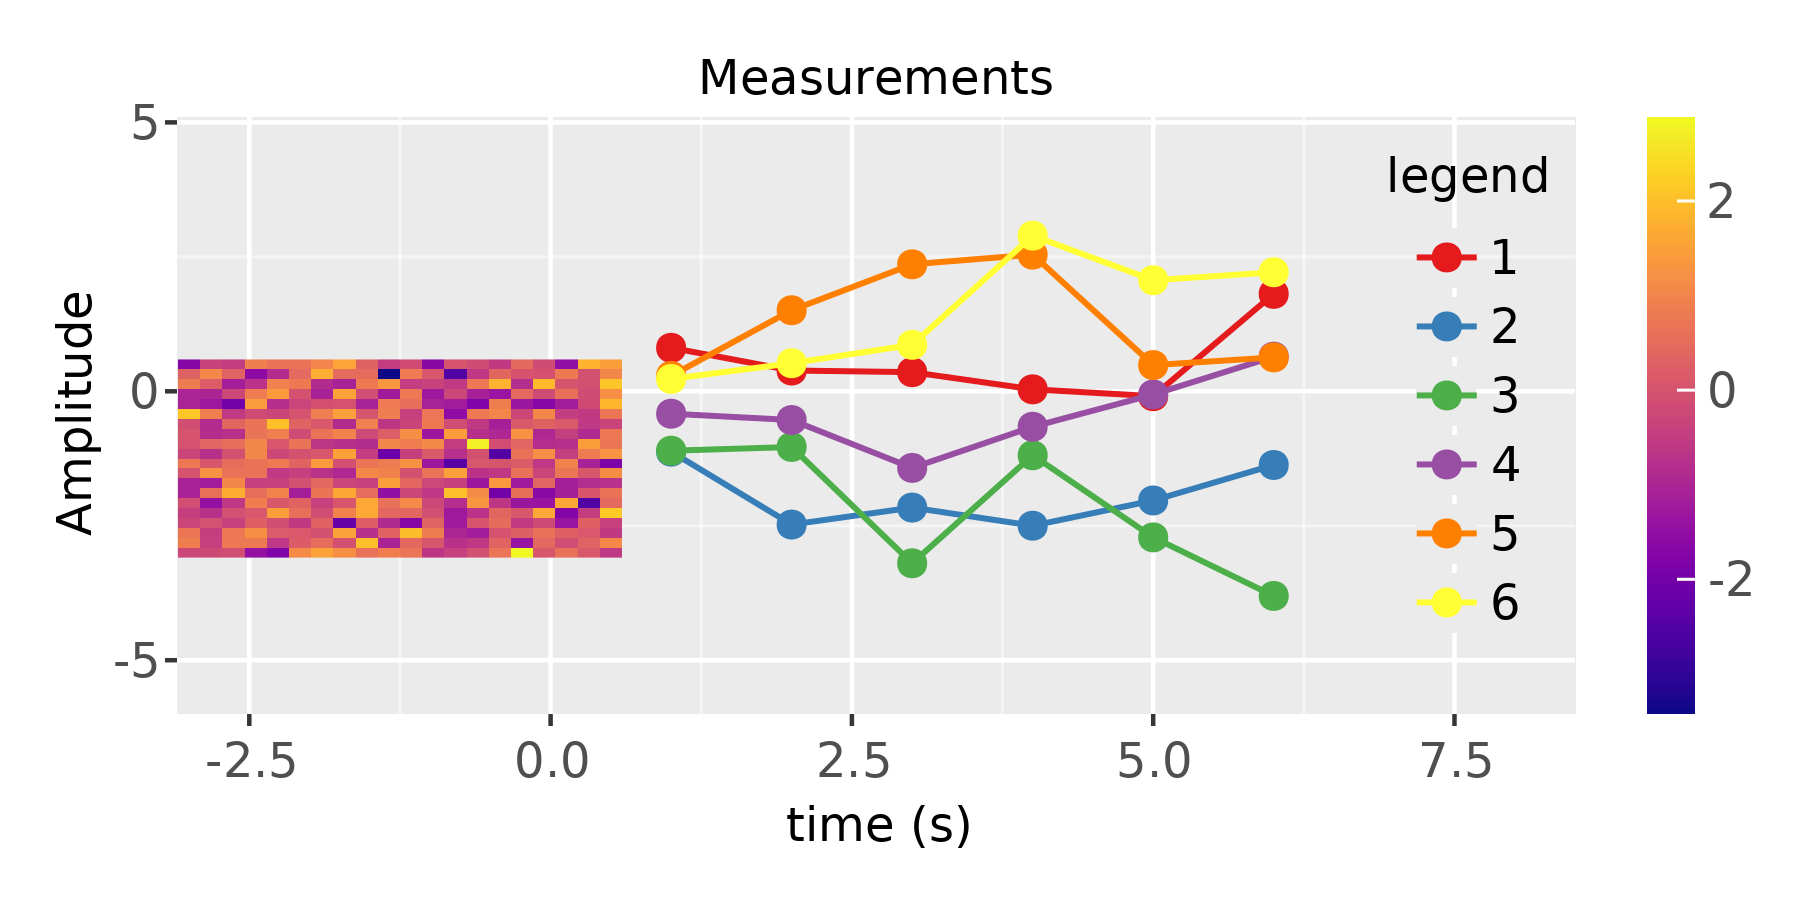
\includegraphics[width=0.6\textwidth,height=\textheight]{_build/im/theme_ggplot2.png}
\caption{Theme ggplot2.}\label{fig:theme_ggplot2}
}
\end{figure}

\begin{figure}
\hypertarget{fig:theme_minimal}{%
\centering
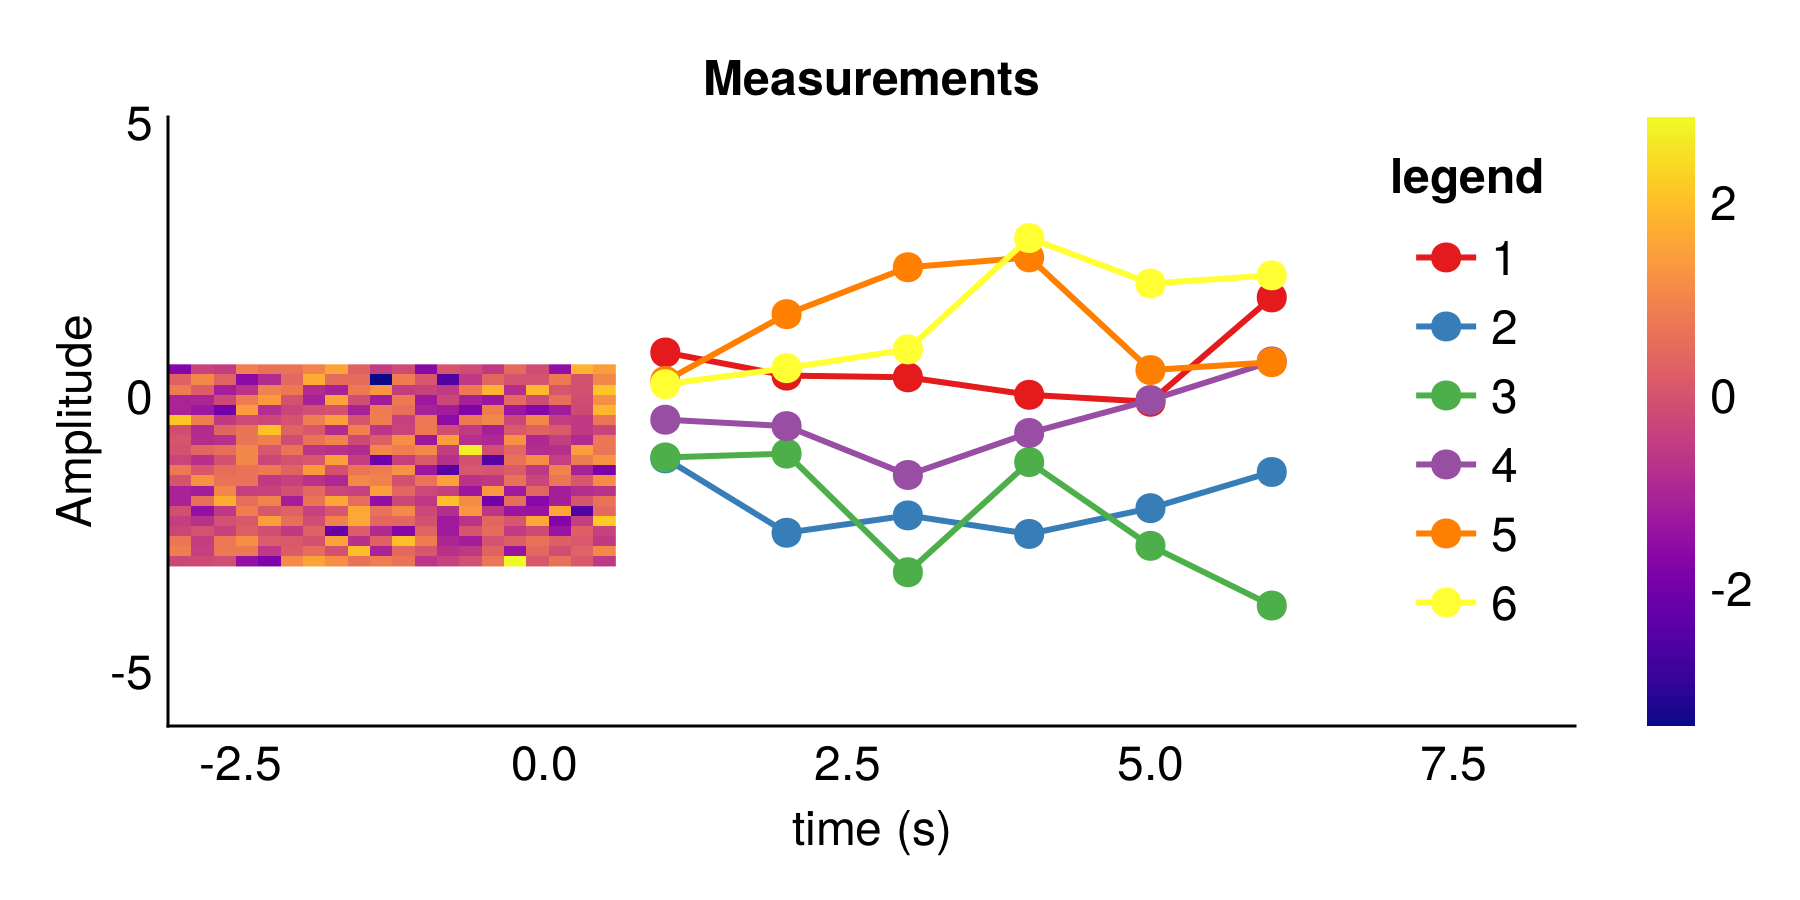
\includegraphics[width=0.6\textwidth,height=\textheight]{_build/im/theme_minimal.png}
\caption{Theme minimal.}\label{fig:theme_minimal}
}
\end{figure}

\begin{figure}
\hypertarget{fig:theme_light}{%
\centering
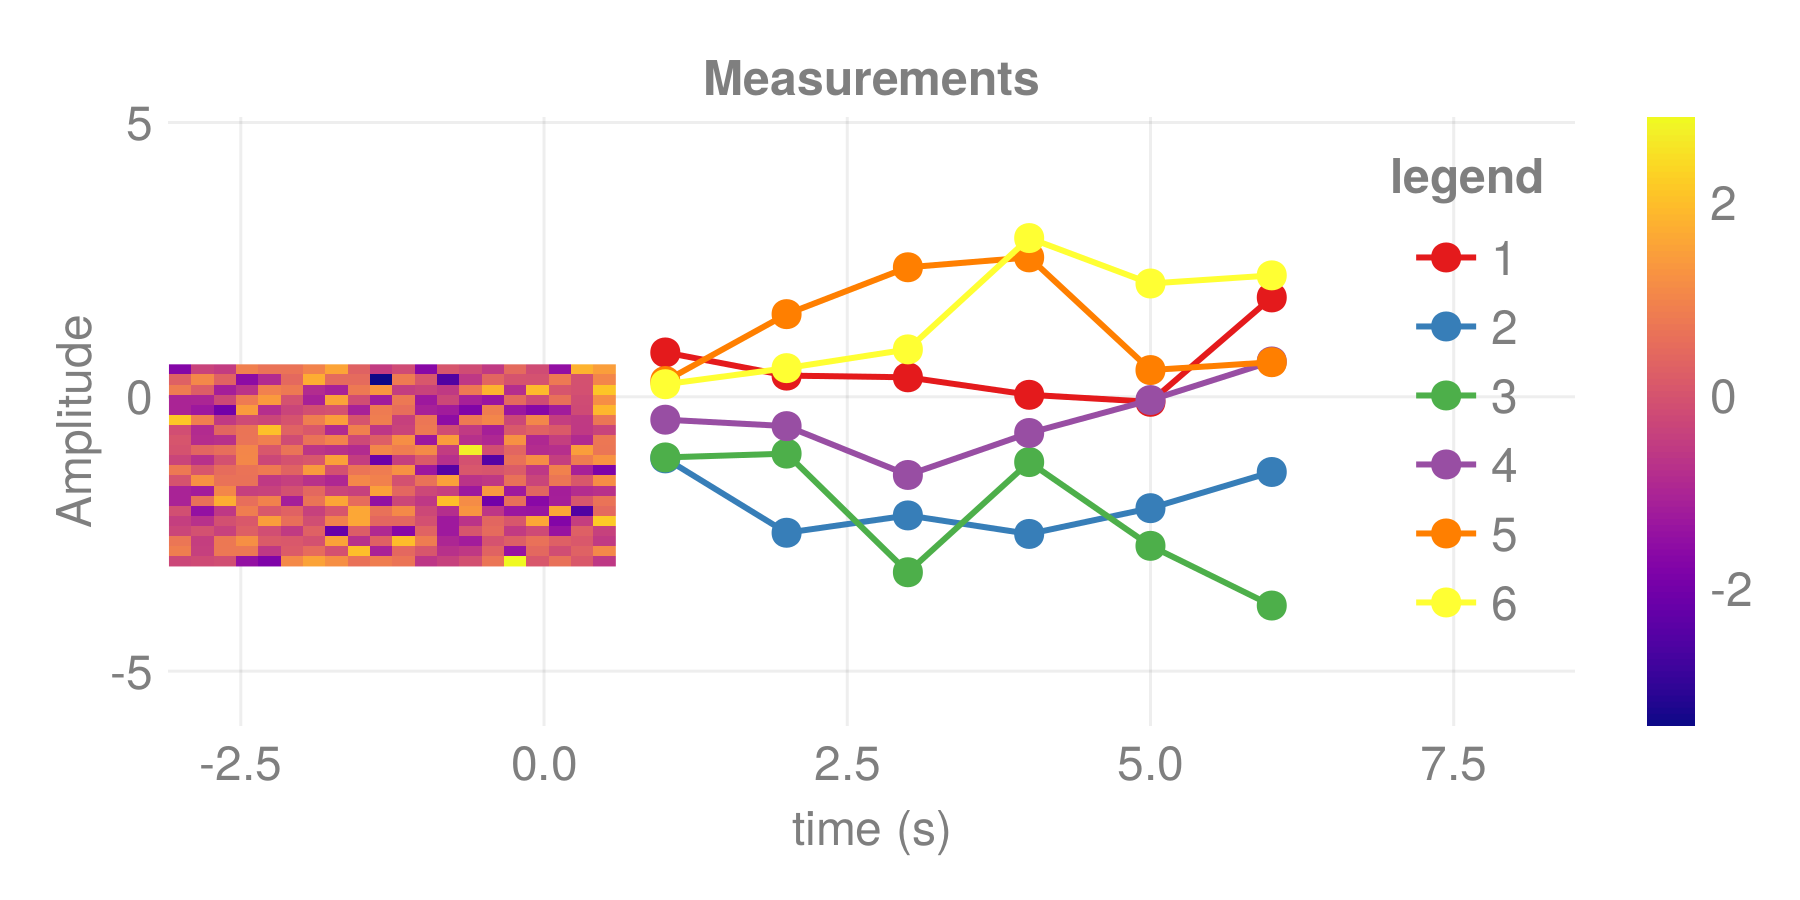
\includegraphics[width=0.6\textwidth,height=\textheight]{_build/im/theme_light.png}
\caption{Theme light.}\label{fig:theme_light}
}
\end{figure}

Another alternative is defining a custom \passthrough{\lstinline!Theme!}
by doing
\passthrough{\lstinline!with\_theme(your\_plot, your\_theme())!}. For
instance, the following theme could be a simple version for a
publication quality template:

\begin{lstlisting}[language=Julia]
publication_theme() = Theme(
    fontsize=16, font="CMU Serif",
    Axis=(xlabelsize=20, xgridstyle=:dash, ygridstyle=:dash,
        xtickalign=1, ytickalign=1, yticksize=10, xticksize=10,
        xlabelpadding=-5, xlabel="x", ylabel="y"),
    Legend=(framecolor=(:black, 0.5), bgcolor=(:white, 0.5)),
    Colorbar=(ticksize=16, tickalign=1, spinewidth=0.5),
)
\end{lstlisting}

Which, for simplicity we use it to plot
\passthrough{\lstinline!scatterlines!} and a
\passthrough{\lstinline!heatmap!}.

\begin{lstlisting}[language=Julia]
function plot_with_legend_and_colorbar()
    fig, ax, _ = scatterlines(1:10; label="line")
    hm = heatmap!(ax, LinRange(6, 9, 15), LinRange(2, 5, 15), randn(15, 15);
        colormap=:Spectral_11)
    axislegend("legend"; position=:lt)
    Colorbar(fig[1, 2], hm, label="values")
    colsize!(fig.layout, 1, Aspect(1, 1.0))
    ax.title = "my custom theme"
    fig
end
\end{lstlisting}

Then, using the previously define \passthrough{\lstinline!Theme!} the
output is shown in Figure
(Figure~\ref{fig:plot_with_legend_and_colorbar}).

\begin{lstlisting}[language=Julia]
with_theme(plot_with_legend_and_colorbar, publication_theme())
\end{lstlisting}

\begin{figure}
\hypertarget{fig:plot_with_legend_and_colorbar}{%
\centering
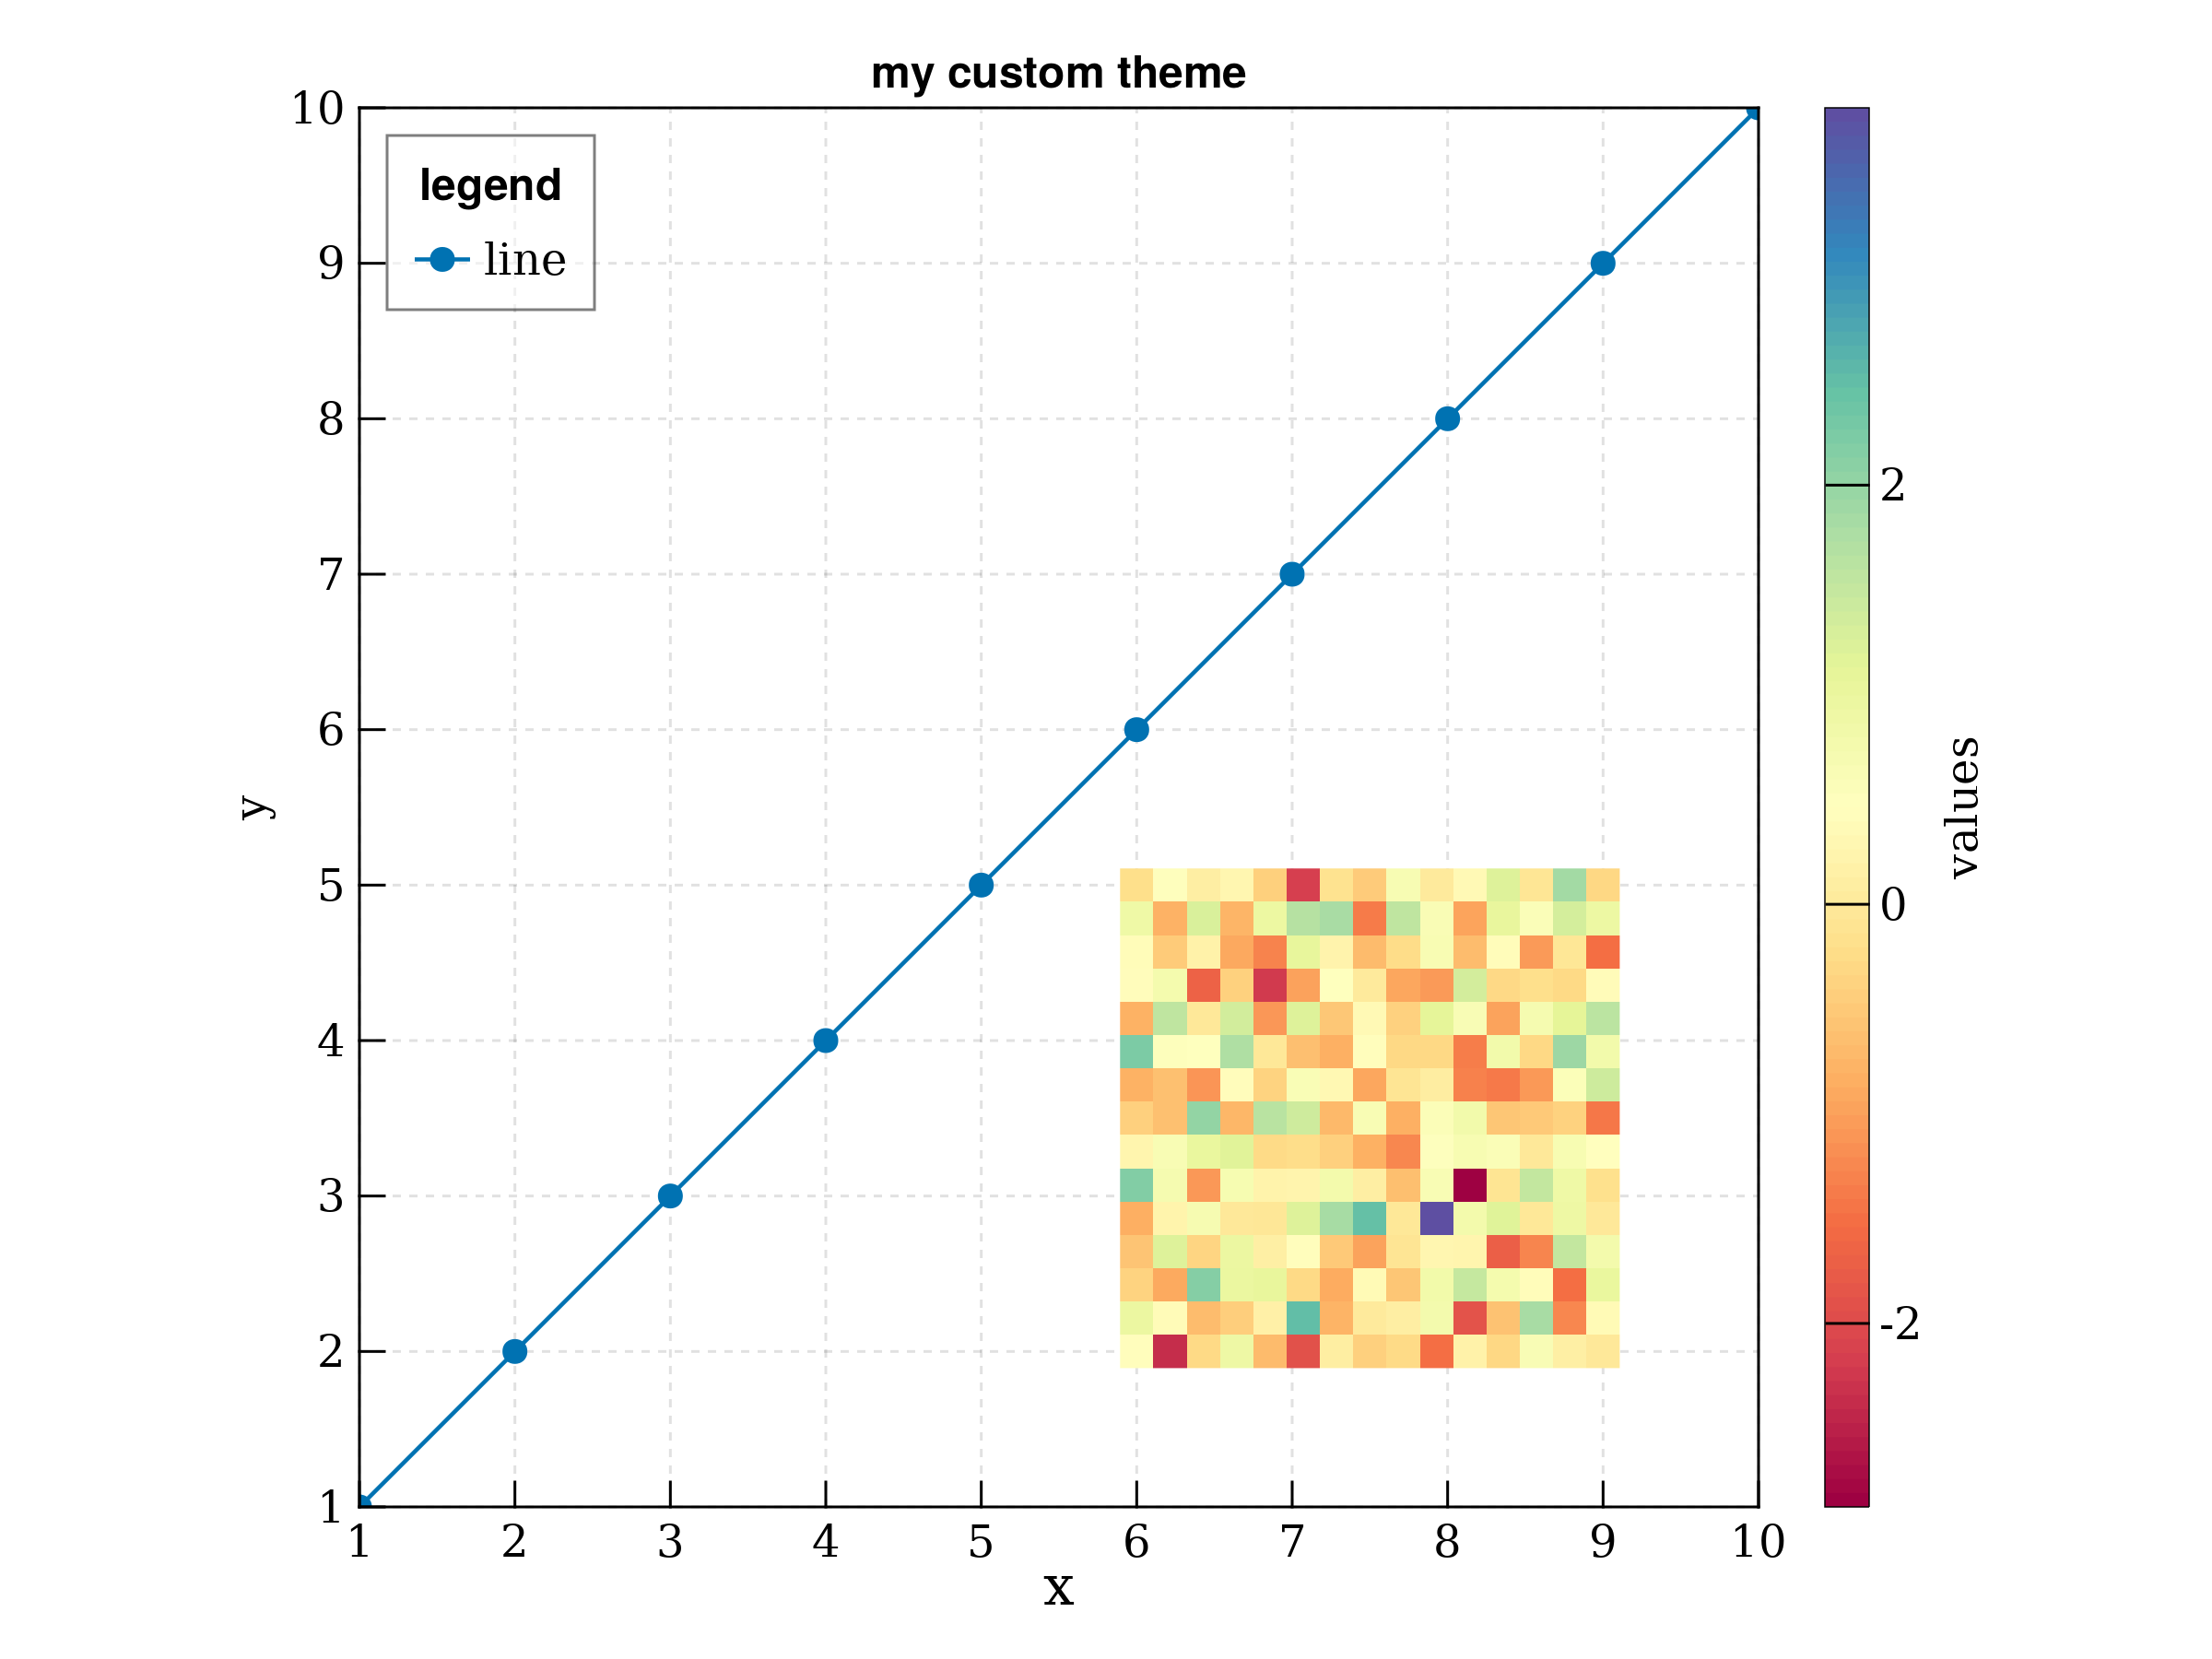
\includegraphics[width=0.6\textwidth,height=\textheight]{_build/im/plot_with_legend_and_colorbar.png}
\caption{Themed plot with Legend and
Colorbar.}\label{fig:plot_with_legend_and_colorbar}
}
\end{figure}

Here we have use \passthrough{\lstinline!with\_theme!} which is more
convenient for the direct application of a theme than the
\passthrough{\lstinline!do!} syntax. You should use the latter if you
want to include extra arguments to the theme that is going to be
applied.

Now, if something needs to be changed after
\passthrough{\lstinline"set\_theme!(your\_theme)"}, we can do it with
\passthrough{\lstinline"update\_theme!(resolution=(500, 400), fontsize=18)"},
for example. Another approach will be to pass additional arguments to
the \passthrough{\lstinline!with\_theme!} function:

\begin{lstlisting}[language=Julia]
fig = (resolution=(600, 400), figure_padding=1, backgroundcolor=:grey90)
ax = (; aspect=DataAspect(), xlabel=L"x", ylabel=L"y")
cbar = (; height=Relative(4 / 5))
with_theme(publication_theme(); fig..., Axis=ax, Colorbar=cbar) do
    plot_with_legend_and_colorbar()
end
\end{lstlisting}

\begin{figure}
\hypertarget{fig:plot_theme_extra_args}{%
\centering
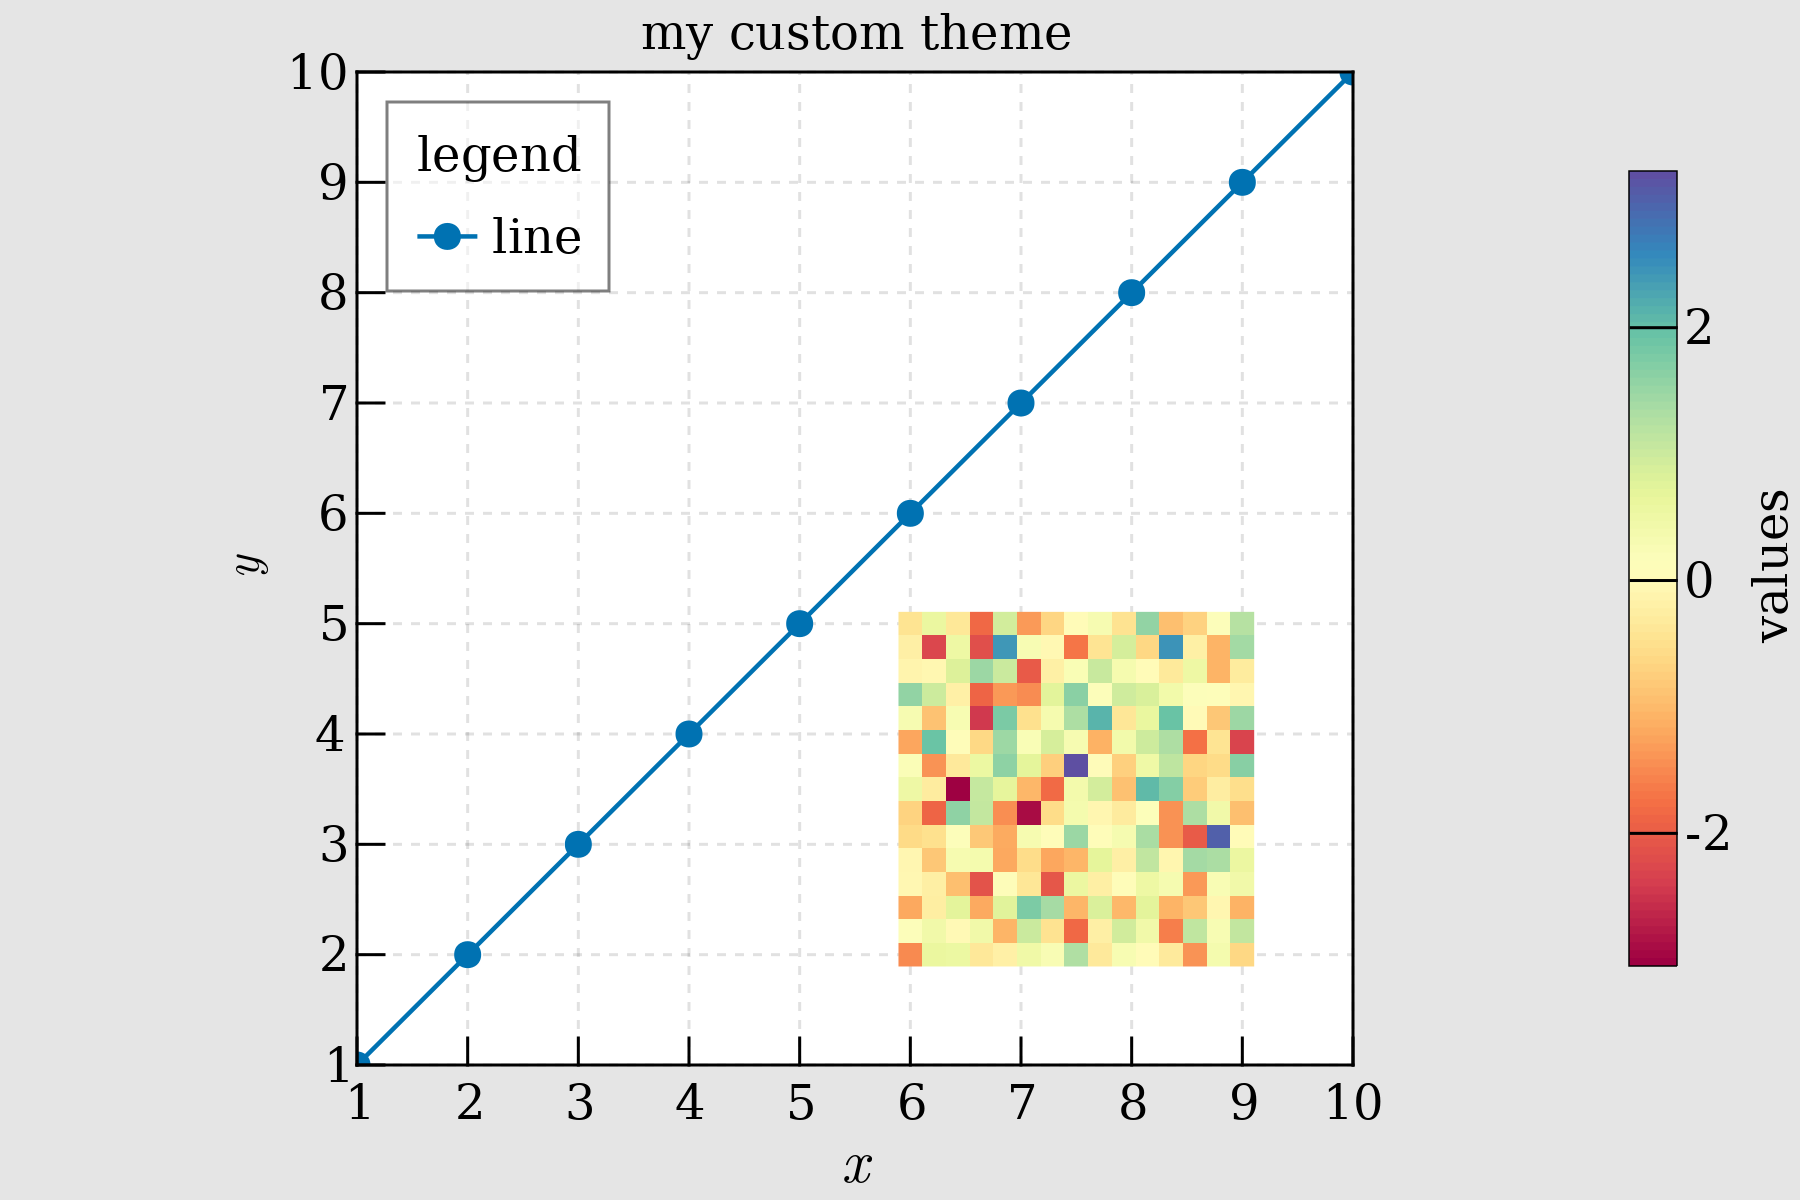
\includegraphics[width=0.6\textwidth,height=\textheight]{_build/im/plot_theme_extra_args.png}
\caption{Theme with extra args.}\label{fig:plot_theme_extra_args}
}
\end{figure}

Where the x and y labels have a Latex format due to
\passthrough{\lstinline!L"..."!}. Most basic Latex strings are already
supported by Makie, however to fully exploit this integration is
recommend to also load the package LaTeXStrings as stated in the next
section.

\hypertarget{using-latexstrings.jl}{%
\section{Using LaTeXStrings.jl}\label{using-latexstrings.jl}}

LaTeX support in \passthrough{\lstinline!Makie.jl!} is also available
via \passthrough{\lstinline!LaTeXStrings.jl!}:

\begin{lstlisting}
using LaTeXStrings
\end{lstlisting}

Simple use cases are shown below (Figure~\ref{fig:latex_strings}). A
basic example includes LaTeX strings for x-y labels and legends:

\begin{lstlisting}[language=Julia]
function LaTeX_Strings()
    x = 0:0.05:4π
    lines(x, x -> sin(3x) / (cos(x) + 2) / x; label=L"\frac{\sin(3x)}{x(\cos(x)+2)}",
        figure=(; resolution=(600, 400)), axis=(; xlabel=L"x"))
    lines!(x, x -> cos(x) / x; label=L"\cos(x)/x")
    lines!(x, x -> exp(-x); label=L"e^{-x}")
    limits!(-0.5, 13, -0.6, 1.05)
    axislegend(L"f(x)")
    current_figure()
end
\end{lstlisting}

\begin{lstlisting}[language=Julia]
with_theme(LaTeX_Strings, publication_theme())
\end{lstlisting}

\begin{figure}
\hypertarget{fig:latex_strings}{%
\centering
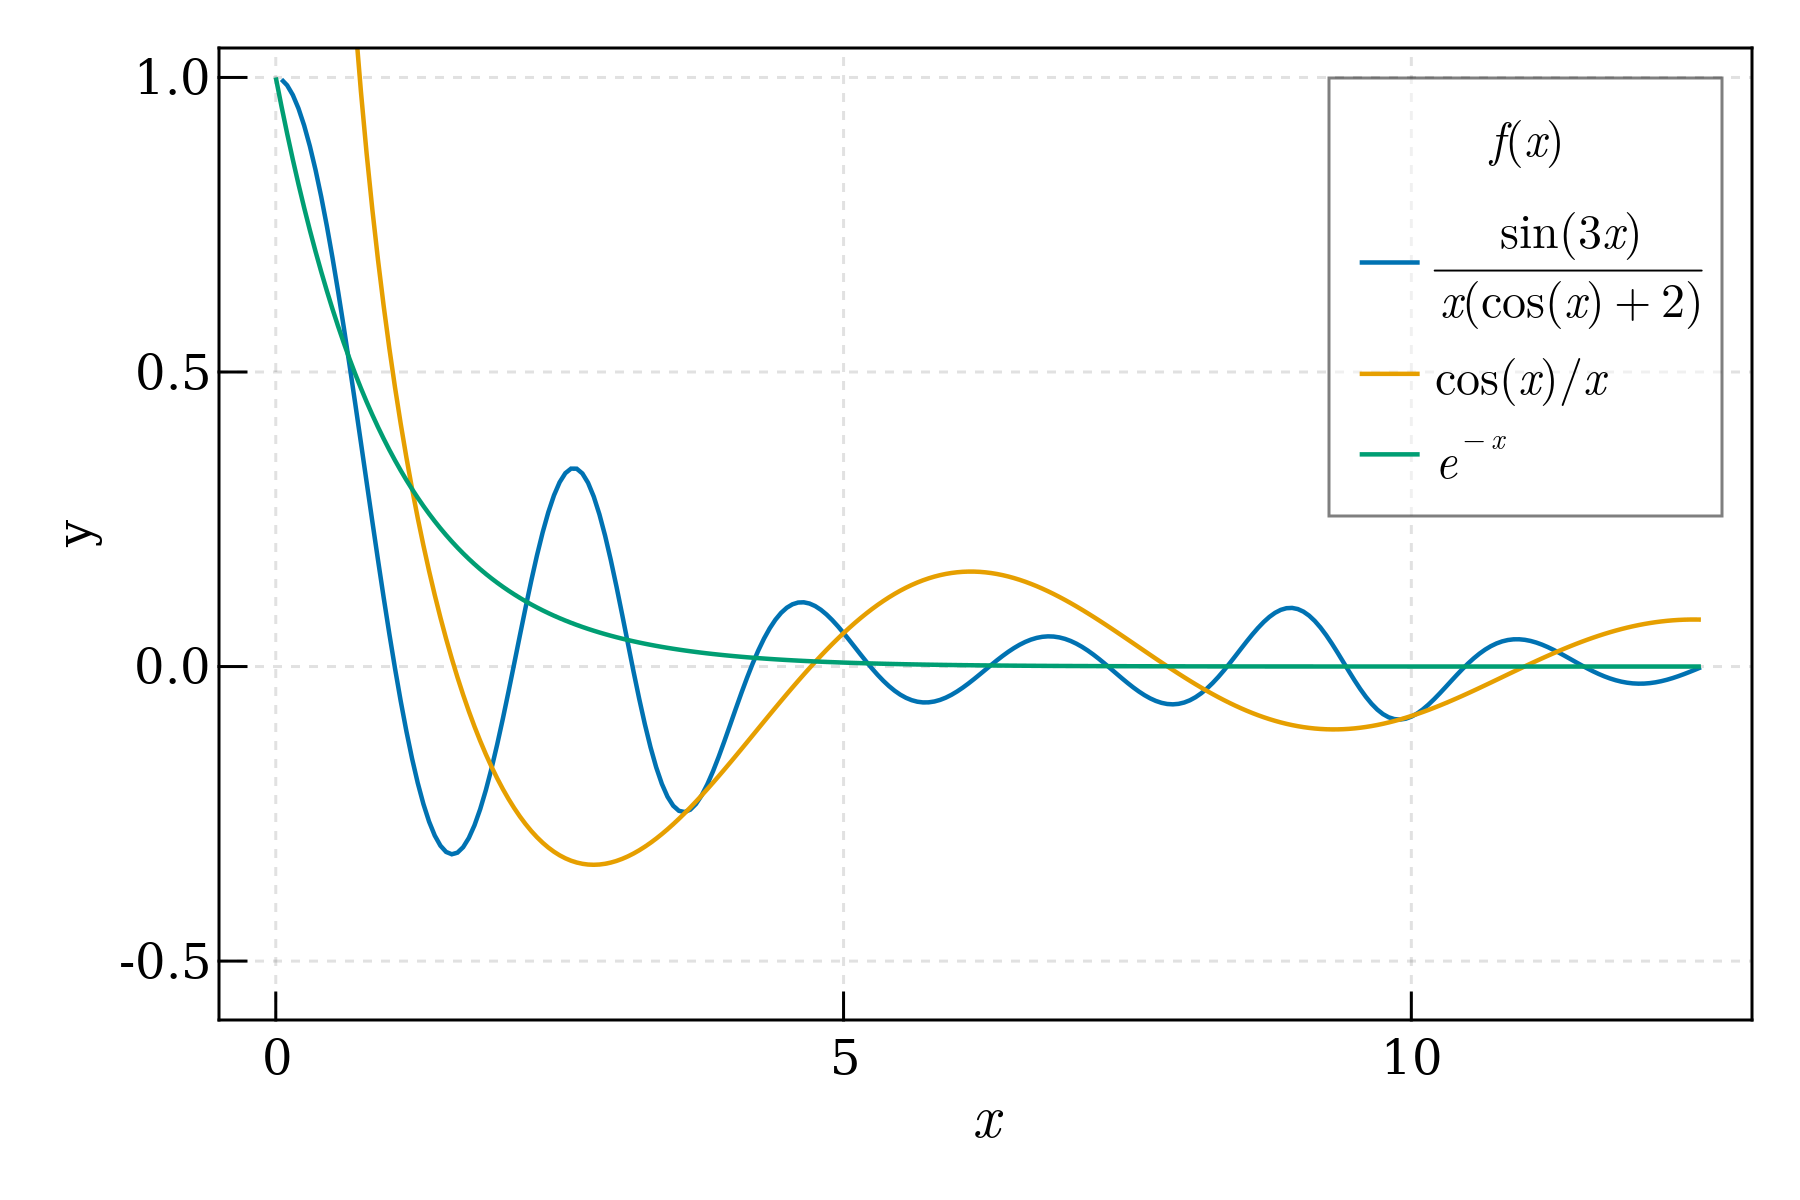
\includegraphics[width=0.6\textwidth,height=\textheight]{_build/im/latex_strings.png}
\caption{Plot with LaTeX strings.}\label{fig:latex_strings}
}
\end{figure}

A more involved example will be one with some equation as
\passthrough{\lstinline!text!} and increasing legend numbering for
curves in a plot:

\begin{lstlisting}[language=Julia]
function multiple_lines()
    x = collect(0:10)
    fig = Figure(resolution=(600, 400), font="CMU Serif")
    ax = Axis(fig[1, 1], xlabel=L"x", ylabel=L"f(x,a)")
    for i = 0:10
        lines!(ax, x, i .* x; label=latexstring("$(i) x"))
    end
    axislegend(L"f(x)"; position=:lt, nbanks=2, labelsize=14)
    text!(L"f(x,a) = ax", position=(4, 80))
    fig
end
multiple_lines()
\end{lstlisting}

\begin{figure}
\hypertarget{fig:multiple_lines}{%
\centering
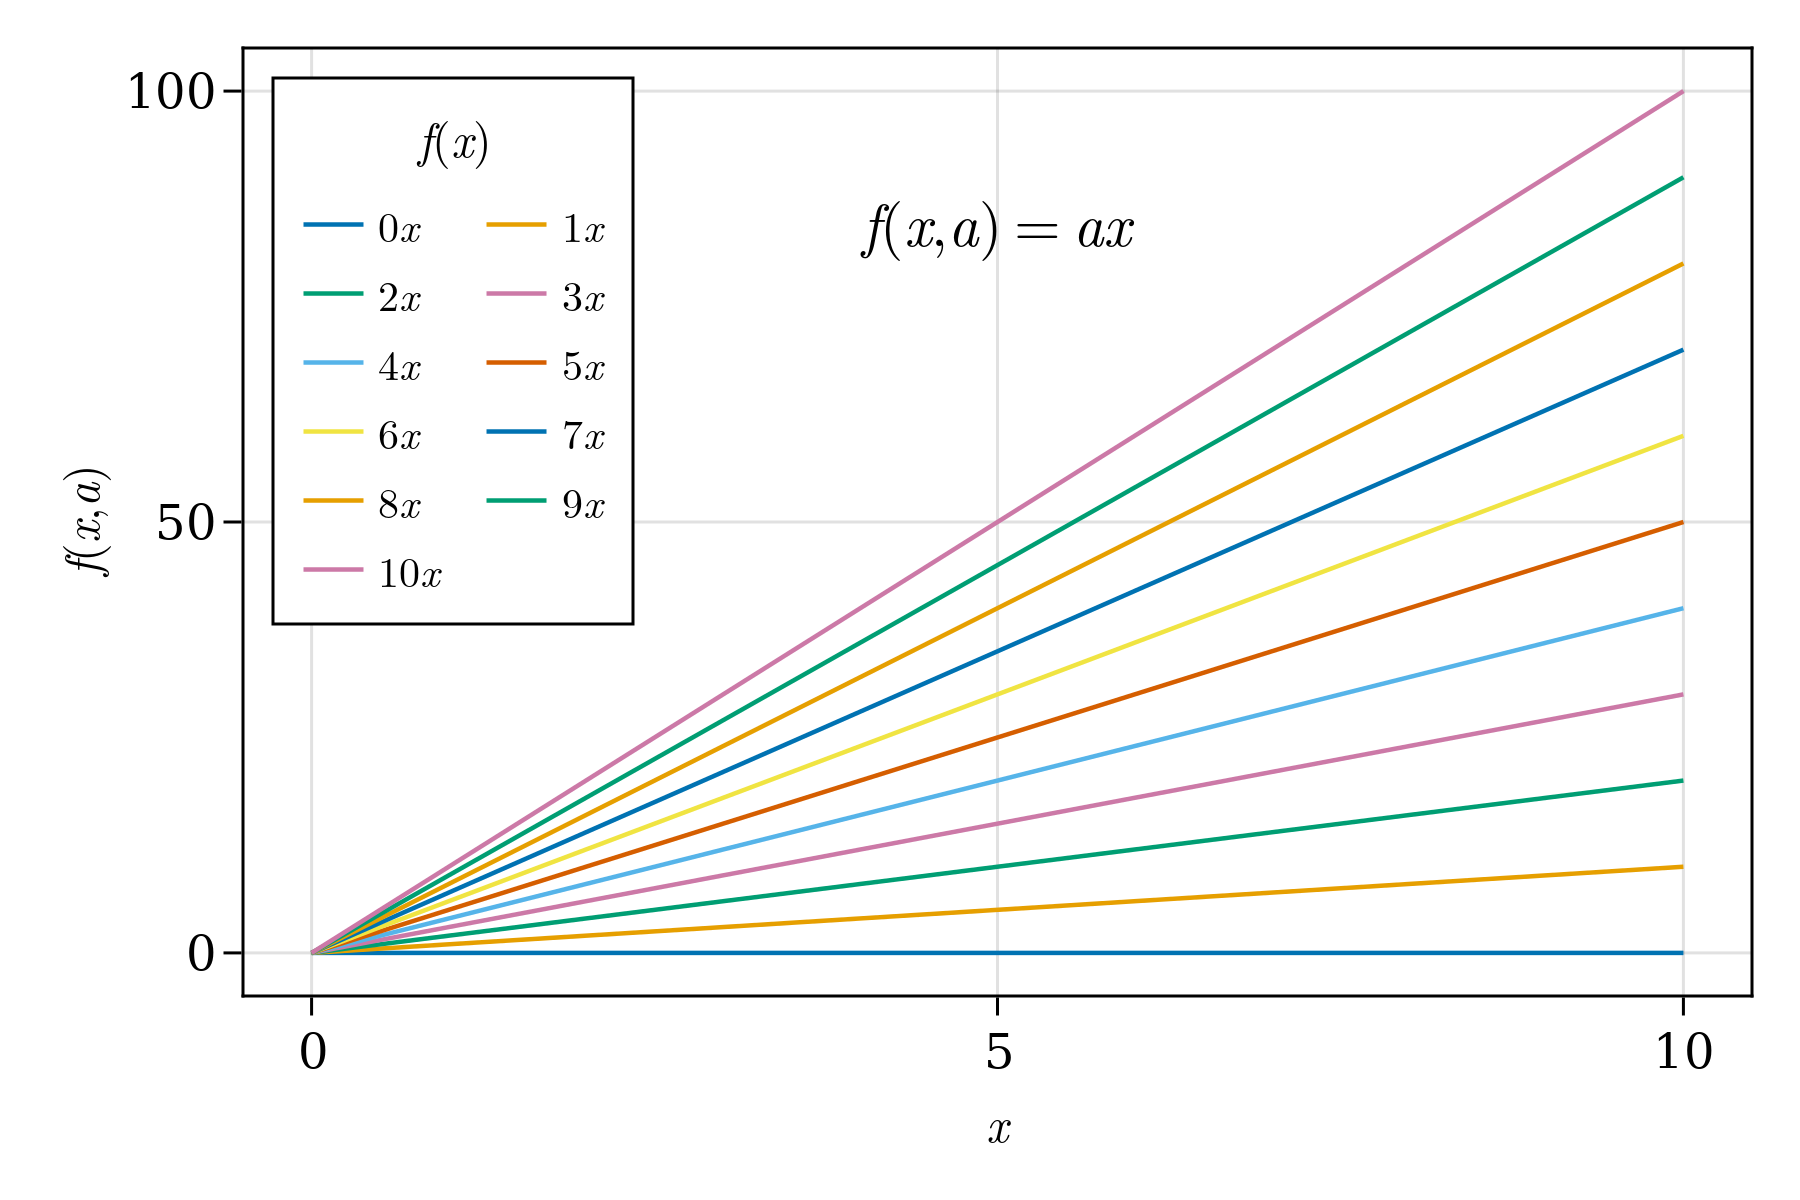
\includegraphics[width=0.6\textwidth,height=\textheight]{_build/im/JDS_multiple_lines_.png}
\caption{Multiple lines.}\label{fig:multiple_lines}
}
\end{figure}

Where \passthrough{\lstinline!latexstring!} from
\passthrough{\lstinline!LaTeXStrings.jl!} has been used to parse the
string. An alternative to this simple case is
\passthrough{\lstinline!L"\%$i x"!}, which is used in the next example.

But, before that there is another problem, some lines have repeated
colors and that's no good. Adding some markers and line styles usually
helps. So, let's do that using
\href{http://makie.juliaplots.org/stable/documentation/theming/index.html\#cycles}{Cycles}
for these types. Setting \passthrough{\lstinline!covary=true!} allows to
cycle all elements together:

\begin{lstlisting}[language=Julia]
function multiple_scatters_and_lines()
    x = collect(0:10)
    cycle = Cycle([:color, :linestyle, :marker], covary=true)
    set_theme!(Lines=(cycle=cycle,), Scatter=(cycle=cycle,))
    fig = Figure(resolution=(600, 400), font="CMU Serif")
    ax = Axis(fig[1, 1], xlabel=L"x", ylabel=L"f(x,a)")
    for i in x
        lines!(ax, x, i .* x; label=L"%$i x")
        scatter!(ax, x, i .* x; markersize=13, strokewidth=0.25,
            label=L"%$i x")
    end
    axislegend(L"f(x)"; merge=true, position=:lt, nbanks=2, labelsize=14)
    text!(L"f(x,a) = ax", position=(4, 80))
    set_theme!() # reset to default theme
    fig
end
multiple_scatters_and_lines()
\end{lstlisting}

\begin{figure}
\hypertarget{fig:multiple_scatters_and_lines}{%
\centering
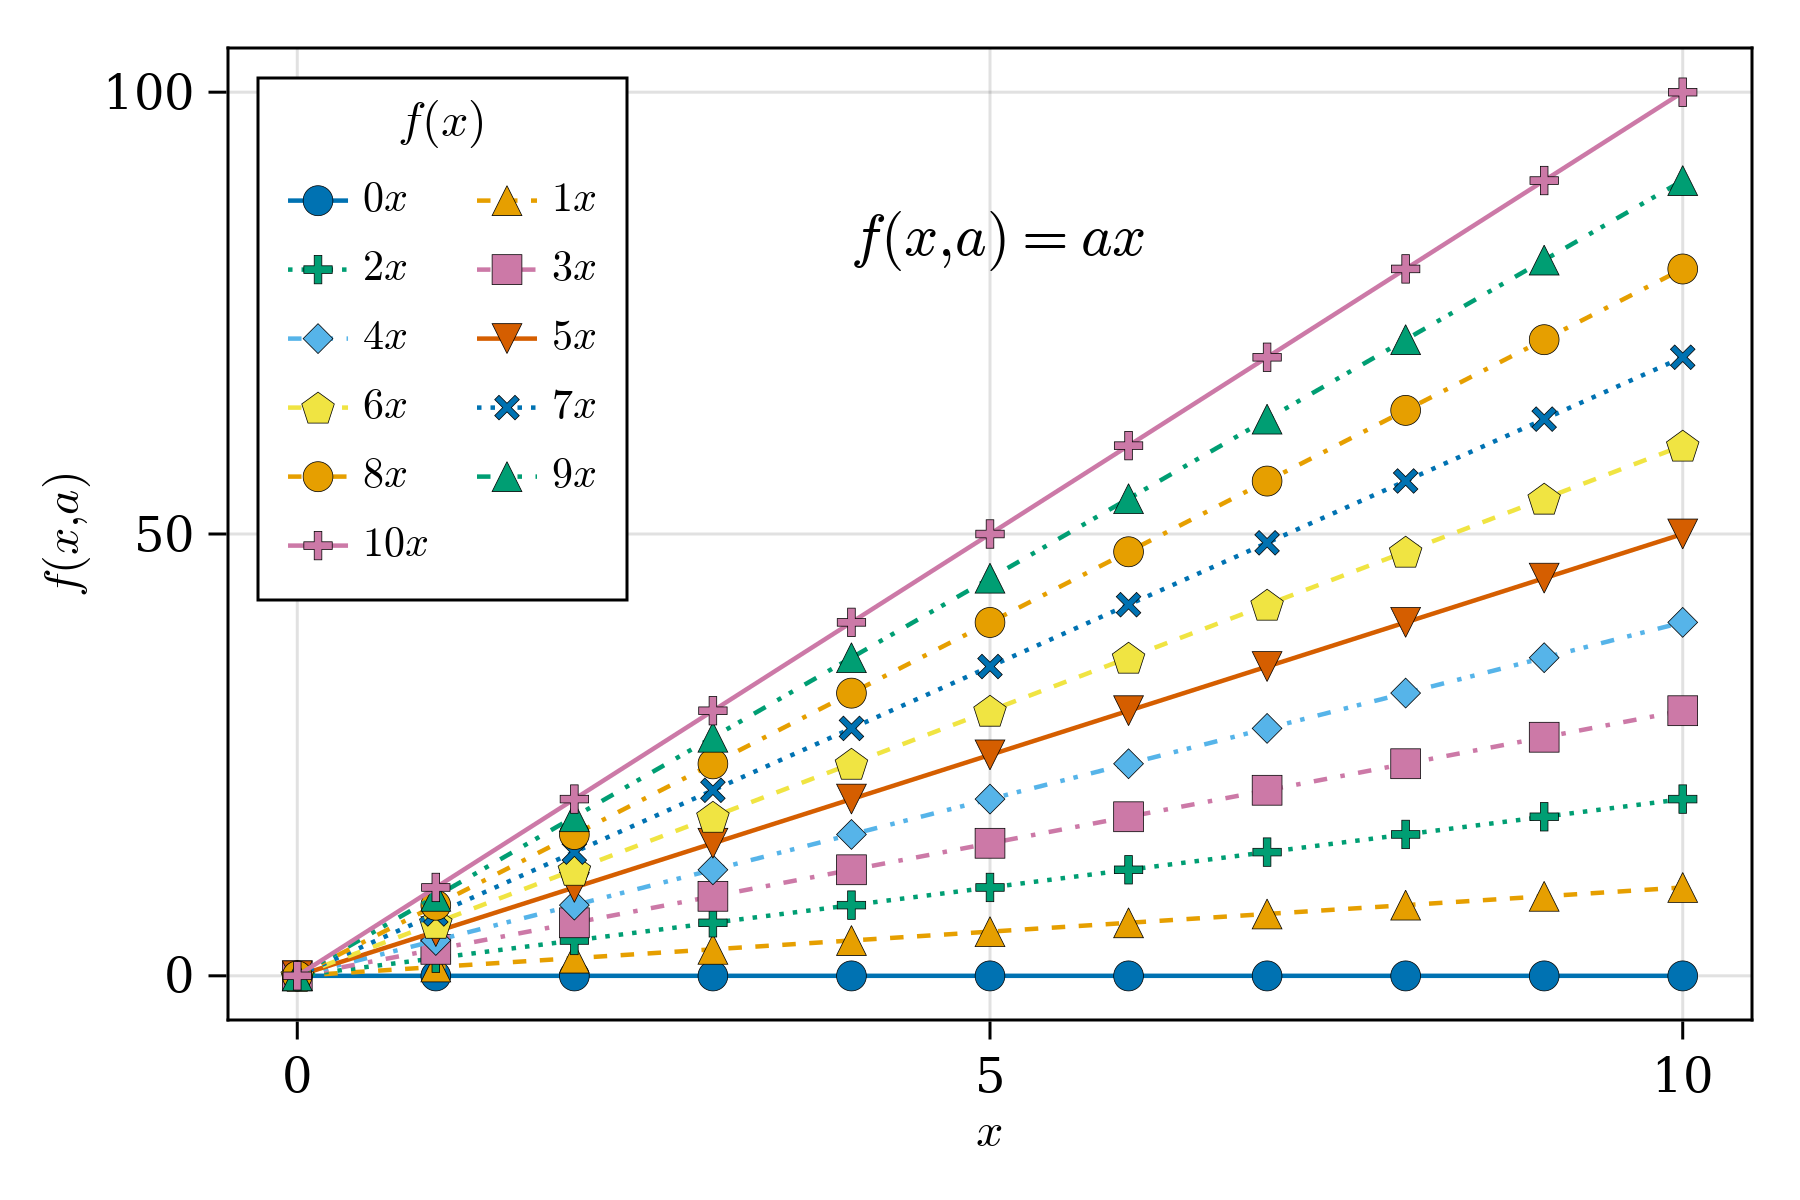
\includegraphics[width=0.6\textwidth,height=\textheight]{_build/im/JDS_multiple_scatters_and_lines_.png}
\caption{Multiple Scatters and
Lines.}\label{fig:multiple_scatters_and_lines}
}
\end{figure}

And voilà. A publication quality plot is here. What more can we ask for?
Well, what about different default colors or palettes. In our next
section, we will see how to use again
\href{http://makie.juliaplots.org/stable/documentation/theming/index.html\#cycles}{Cycles}
and know a little bit more about them, plus some additional keywords in
order to achieve this.

\hypertarget{sec:makie_colors}{%
\section{Colors and Colormaps}\label{sec:makie_colors}}

Choosing an appropriate set of colors or colorbar for your plot is an
essential part when presenting results. Using
\href{https://github.com/JuliaGraphics/Colors.jl}{Colors.jl} is
supported in \passthrough{\lstinline!Makie.jl!} so that you can use
\href{https://juliagraphics.github.io/Colors.jl/latest/namedcolors/}{named
colors} or pass \passthrough{\lstinline!RGB!} or
\passthrough{\lstinline!RGBA!} values. Additionally, colormaps from
\href{https://github.com/JuliaGraphics/ColorSchemes.jl}{ColorSchemes.jl}
and
\href{https://github.com/peterkovesi/PerceptualColourMaps.jl}{PerceptualColourMaps.jl}
can also be used. It is worth knowing that you can reverse a colormap by
doing \passthrough{\lstinline!Reverse(:colormap\_name)!} and obtain a
transparent color or colormap with
\passthrough{\lstinline!color=(:red,0.5)!} and
\passthrough{\lstinline!colormap=(:viridis, 0.5)!}.

Different use cases will be shown next. Then we will define a custom
theme with new colors and a colorbar palette.

By default \passthrough{\lstinline!Makie.jl!} has a predefined set of
colors in order to cycle through them automatically, as shown in the
previous figures, where no specific color was set. Overwriting these
defaults is done by calling the keyword \passthrough{\lstinline!color!}
in the plotting function and specifying a new color via a
\passthrough{\lstinline!Symbol!} or \passthrough{\lstinline!String!}.
See this in action in the following example:

\begin{lstlisting}[language=Julia]
function set_colors_and_cycle()
    # Epicycloid lines
    x(r, k, θ) = r * (k .+ 1.0) .* cos.(θ) .- r * cos.((k .+ 1.0) .* θ)
    y(r, k, θ) = r * (k .+ 1.0) .* sin.(θ) .- r * sin.((k .+ 1.0) .* θ)
    θ = LinRange(0, 6.2π, 1000)
    axis = (; xlabel=L"x(\theta)", ylabel=L"y(\theta)",
        title="Epicycloid", aspect=DataAspect())
    figure = (; resolution=(600, 400), font="CMU Serif")
    fig, ax, _ = lines(x(1, 1, θ), y(1, 1, θ); color="firebrick1", # string
        label=L"1.0", axis=axis, figure=figure)
    lines!(ax, x(4, 2, θ), y(4, 2, θ); color=:royalblue1, #symbol
        label=L"2.0")
    for k = 2.5:0.5:5.5
        lines!(ax, x(2k, k, θ), y(2k, k, θ); label=latexstring("$(k)")) #cycle
    end
    Legend(fig[1, 2], ax, latexstring("k, r = 2k"), merge=true)
    colsize!(fig.layout, 1, Aspect(1, 1.0))
    fig
end
set_colors_and_cycle()
\end{lstlisting}

\begin{figure}
\hypertarget{fig:set_colors_and_cycle}{%
\centering
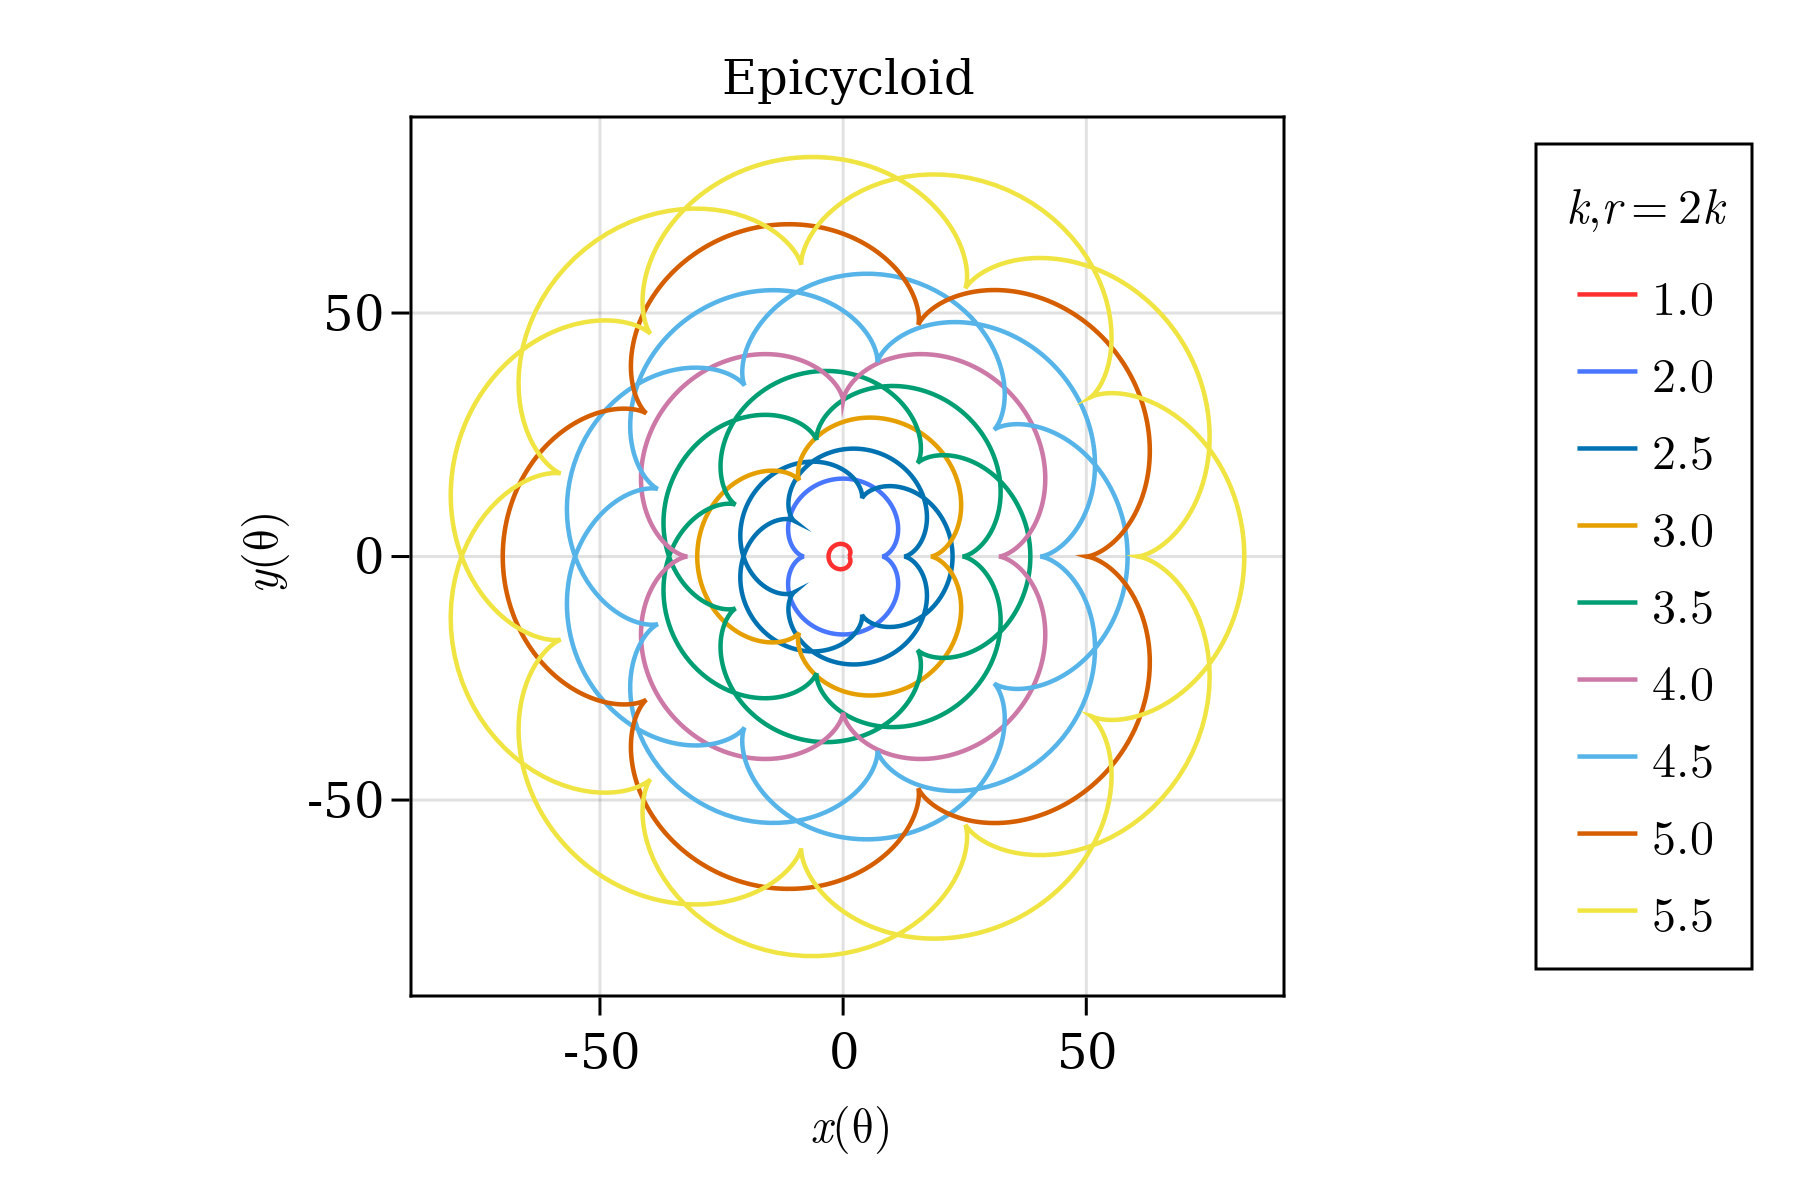
\includegraphics{_build/im/JDS_set_colors_and_cycle_.png}
\caption{Set colors and cycle.}\label{fig:set_colors_and_cycle}
}
\end{figure}

Where, in the first two lines we have used the keyword
\passthrough{\lstinline!color!} to specify our color. The rest is using
the default cycle set of colors. Later, we will learn how to do a custom
cycle.

Regarding colormaps, we are already familiar with the keyword
\passthrough{\lstinline!colormap!} for heatmaps and scatters. Here, we
show that a colormap can also be specified via a
\passthrough{\lstinline!Symbol!} or a \passthrough{\lstinline!String!},
similar to colors. Or, even a vector of \passthrough{\lstinline!RGB!}
colors. Let's do our first example by calling colormaps as a
\passthrough{\lstinline!Symbol!}, \passthrough{\lstinline!String!} and
\passthrough{\lstinline!cgrad!} for categorical values. See
\passthrough{\lstinline!?cgrad!} for more information.

\begin{lstlisting}[language=Julia]
figure = (; resolution=(600, 400), font="CMU Serif")
axis = (; xlabel=L"x", ylabel=L"y", aspect=DataAspect())
fig, ax, pltobj = heatmap(rand(20, 20); colorrange=(0, 1),
    colormap=Reverse(:viridis), axis=axis, figure=figure)
Colorbar(fig[1, 2], pltobj, label = "Reverse sequential colormap")
colsize!(fig.layout, 1, Aspect(1, 1.0))
fig
\end{lstlisting}

\begin{figure}
\hypertarget{fig:Reverse_colormap_sequential}{%
\centering
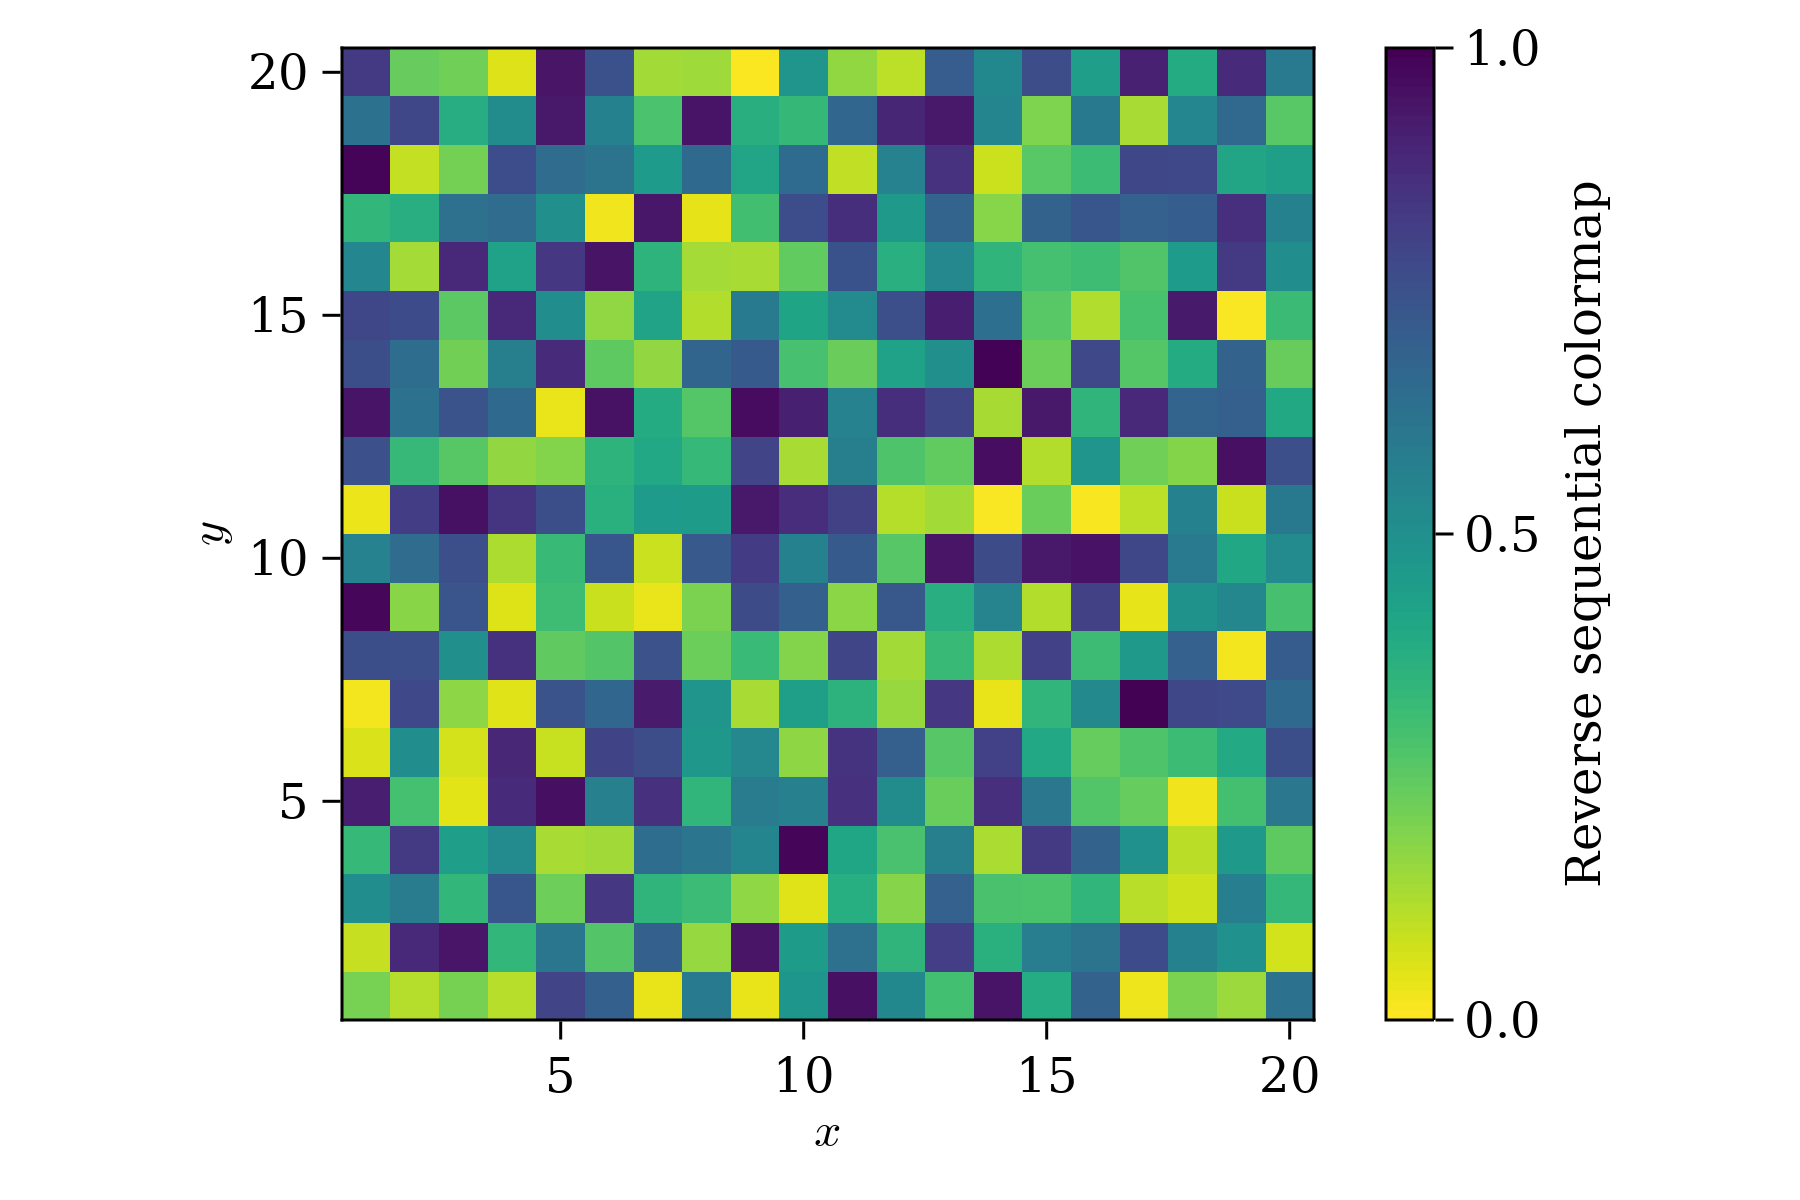
\includegraphics[width=0.6\textwidth,height=\textheight]{_build/im/Reverse_colormap_sequential.png}
\caption{Reverse sequential colormap and
colorrange.}\label{fig:Reverse_colormap_sequential}
}
\end{figure}

When setting a \passthrough{\lstinline!colorrange!} usually the values
outside this range are colored with the first and last color from the
colormap. However, sometimes is better to specify the color you want at
both ends. We do that with \passthrough{\lstinline!highclip!} and
\passthrough{\lstinline!lowclip!}:

\begin{lstlisting}
using ColorSchemes
\end{lstlisting}

\begin{lstlisting}[language=Julia]
figure = (; resolution=(600, 400), font="CMU Serif")
axis = (; xlabel=L"x", ylabel=L"y", aspect=DataAspect())
fig, ax, pltobj=heatmap(randn(20, 20); colorrange=(-2, 2),
    colormap="diverging_rainbow_bgymr_45_85_c67_n256",
    highclip=:black, lowclip=:white, axis=axis, figure=figure)
Colorbar(fig[1, 2], pltobj, label = "Diverging colormap")
colsize!(fig.layout, 1, Aspect(1, 1.0))
fig
\end{lstlisting}

\begin{figure}
\hypertarget{fig:diverging_colormap}{%
\centering
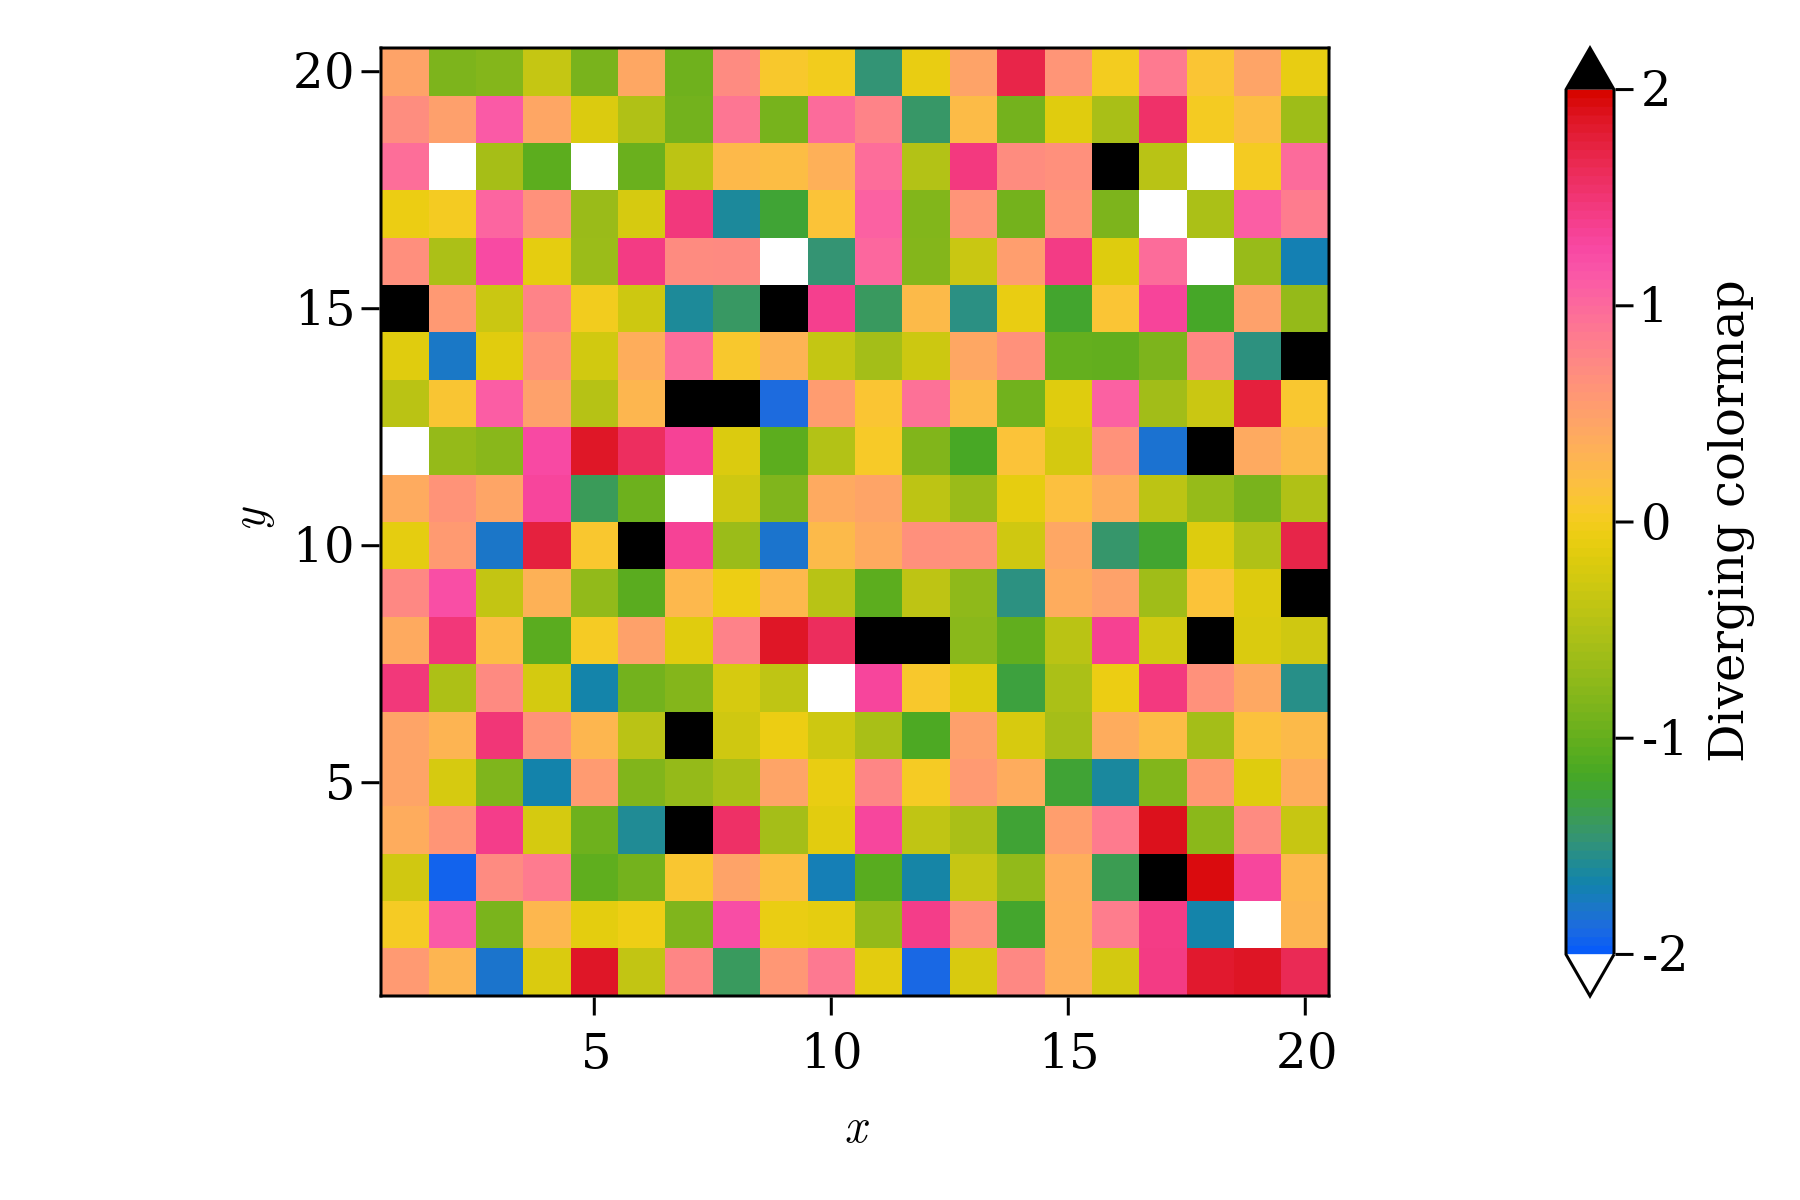
\includegraphics[width=0.6\textwidth,height=\textheight]{_build/im/diverging_colormap.png}
\caption{Diverging Colormap with low and high
clip.}\label{fig:diverging_colormap}
}
\end{figure}

But we mentioned that also \passthrough{\lstinline!RGB!} vectors are
valid options. For our next example you could pass the custom colormap
\emph{perse} or use \passthrough{\lstinline!cgrad!} to force a
categorical \passthrough{\lstinline!Colorbar!}.

\begin{lstlisting}
using Colors, ColorSchemes
\end{lstlisting}

\begin{lstlisting}[language=Julia]
figure = (; resolution=(600, 400), font="CMU Serif")
axis = (; xlabel=L"x", ylabel=L"y", aspect=DataAspect())
#cmap = ColorScheme(range(colorant"red", colorant"green", length=3))
# this is another way to obtain a colormap, not used here, but try it.
mycmap = ColorScheme([RGB{Float64}(i, 1.5i, 2i) for i in [0.0, 0.25, 0.35, 0.5]])
fig, ax, pltobj = heatmap(rand(-1:1, 20, 20);
    colormap=cgrad(mycmap, 3, categorical=true, rev=true), # cgrad and Symbol, mycmap
    axis=axis, figure=figure)
cbar = Colorbar(fig[1, 2], pltobj, label="Categories")
cbar.ticks = ([-0.66, 0, 0.66], ["negative", "neutral", "positive"])
colsize!(fig.layout, 1, Aspect(1, 1.0))
fig
\end{lstlisting}

\begin{figure}
\hypertarget{fig:categorical_colormap}{%
\centering
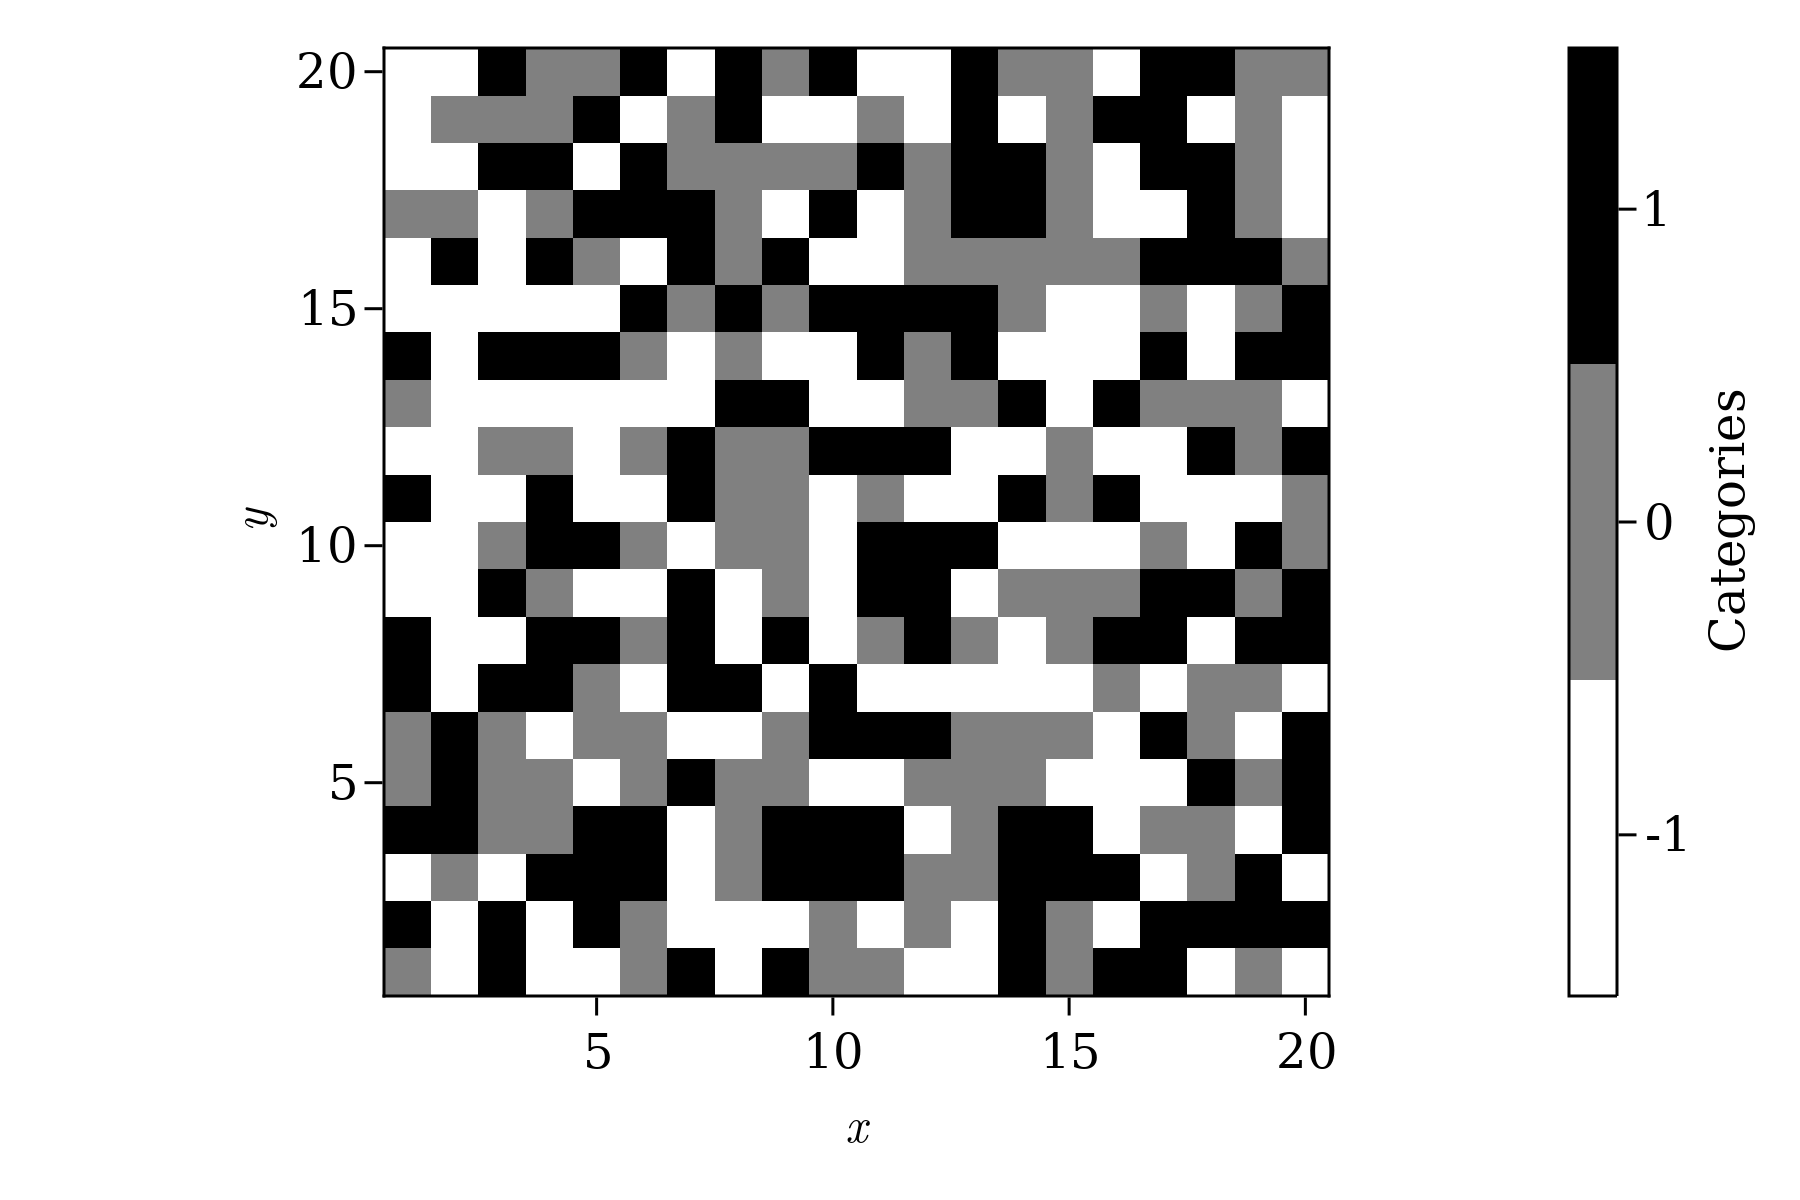
\includegraphics[width=0.6\textwidth,height=\textheight]{_build/im/categorical_colormap.png}
\caption{Categorical Colormap.}\label{fig:categorical_colormap}
}
\end{figure}

Lastly, the ticks in the colorbar for the categorial case are not
centered by default in each color. This is fixed by passing custom
ticks, as in \passthrough{\lstinline!cbar.ticks = (positions, ticks)!}.

The last situation is when passing a multiple colors to
\passthrough{\lstinline!colormap!}. You will get an interpolated
colormap between these two colors. Also, hexadecimal coded colors are
accepted. So, on top or our heatmap let's put one semi-transparent point
using this.

\begin{lstlisting}[language=Julia]
figure = (; resolution=(600, 400), font="CMU Serif")
axis = (; xlabel=L"x", ylabel=L"y", aspect=DataAspect())
fig, ax, pltobj = heatmap(rand(20, 20); colorrange=(0, 1),
    colormap=["red", "black"], axis=axis, figure=figure)
scatter!(ax, [11], [11], color=("#C0C0C0", 0.5), markersize=150)
Colorbar(fig[1, 2], pltobj, label="2 colors")
colsize!(fig.layout, 1, Aspect(1, 1.0))
fig
\end{lstlisting}

\begin{figure}
\hypertarget{fig:colormap_two_colors}{%
\centering
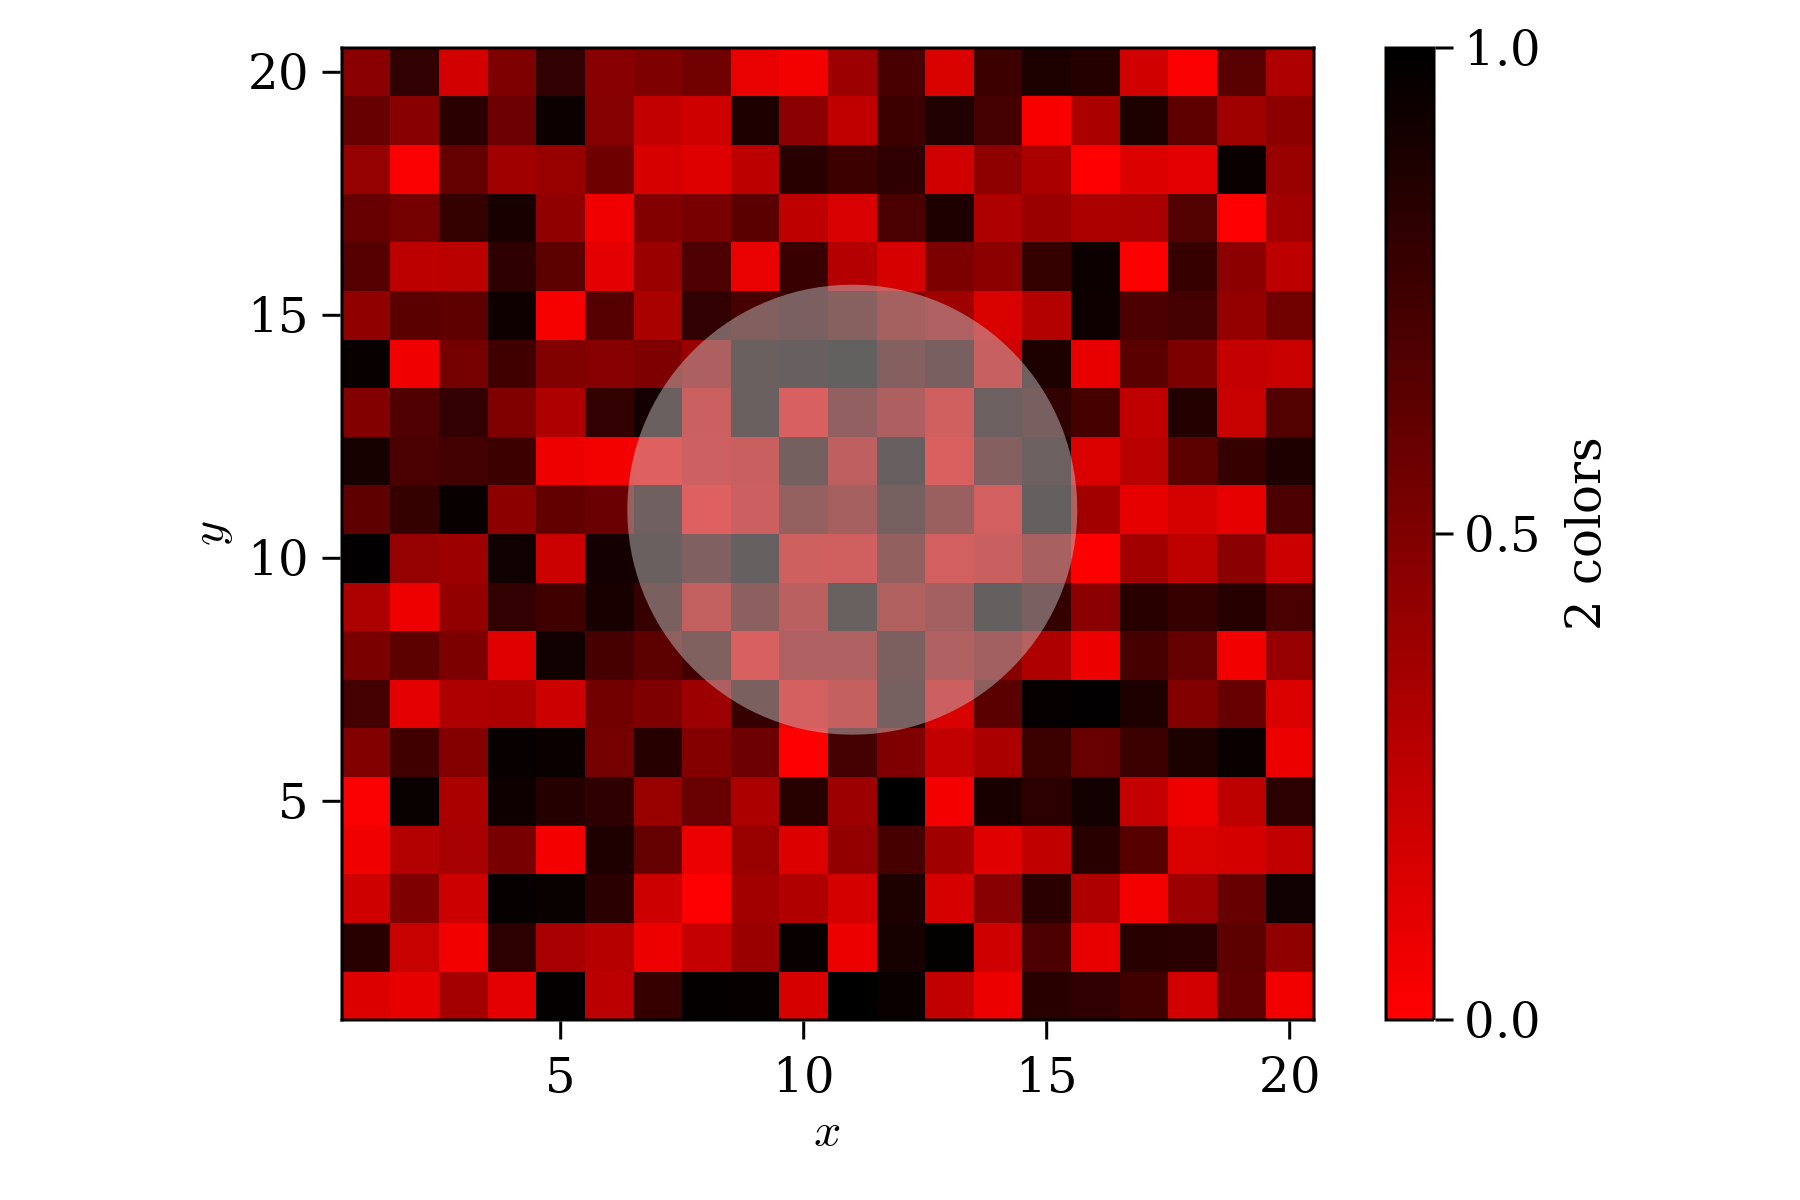
\includegraphics[width=0.6\textwidth,height=\textheight]{_build/im/colormap_two_colors.png}
\caption{Colormap from two colors.}\label{fig:colormap_two_colors}
}
\end{figure}

\hypertarget{custom-cycle}{%
\subsection{Custom cycle}\label{custom-cycle}}

Here, we could define a global \passthrough{\lstinline!Theme!} with a
new cycle for colors, however that is \textbf{not the recommend way} to
do it. It's better to define a new theme and use as shown before. Let's
define a new one with a \passthrough{\lstinline!cycle!} for
\passthrough{\lstinline!:color!}, \passthrough{\lstinline!:linestyle!},
\passthrough{\lstinline!:marker!} and a new
\passthrough{\lstinline!colormap!} default. And add these new attributes
to our previous \passthrough{\lstinline!publication\_theme!}.

\begin{lstlisting}[language=Julia]
function new_cycle_theme()
    # https://nanx.me/ggsci/reference/pal_locuszoom.html
    my_colors = ["#D43F3AFF", "#EEA236FF", "#5CB85CFF", "#46B8DAFF",
        "#357EBDFF", "#9632B8FF", "#B8B8B8FF"]
    cycle = Cycle([:color, :linestyle, :marker], covary=true) # alltogether
    my_markers = [:circle, :rect, :utriangle, :dtriangle, :diamond,
        :pentagon, :cross, :xcross]
    my_linestyle = [nothing, :dash, :dot, :dashdot, :dashdotdot]
    Theme(
        fontsize=16, font="CMU Serif",
        colormap=:linear_bmy_10_95_c78_n256,
        palette=(color=my_colors, marker=my_markers, linestyle=my_linestyle),
        Lines=(cycle=cycle,), Scatter=(cycle=cycle,),
        Axis=(xlabelsize=20, xgridstyle=:dash, ygridstyle=:dash,
            xtickalign=1, ytickalign=1, yticksize=10, xticksize=10,
            xlabelpadding=-5, xlabel="x", ylabel="y"),
        Legend=(framecolor=(:black, 0.5), bgcolor=(:white, 0.5)),
        Colorbar=(ticksize=16, tickalign=1, spinewidth=0.5),
    )
end
\end{lstlisting}

And apply it to a plotting function like the following:

\begin{lstlisting}[language=Julia]
function scatters_and_lines()
    x = collect(0:10)
    xh = LinRange(4, 6, 25)
    yh = LinRange(70, 95, 25)
    h = randn(25, 25)
    fig = Figure(resolution=(600, 400), font="CMU Serif")
    ax = Axis(fig[1, 1], xlabel=L"x", ylabel=L"f(x,a)")
    for i in x
        lines!(ax, x, i .* x; label=latexstring("$(i) x"))
        scatter!(ax, x, i .* x; markersize=13, strokewidth=0.25,
            label=latexstring("$(i) x"))
    end
    hm = heatmap!(xh, yh, h)
    axislegend(L"f(x)"; merge=true, position=:lt, nbanks=2, labelsize=14)
    Colorbar(fig[1, 2], hm, label="new default colormap")
    limits!(ax, -0.5, 10.5, -5, 105)
    colgap!(fig.layout, 5)
    fig
end
\end{lstlisting}

\begin{lstlisting}[language=Julia]
with_theme(scatters_and_lines, new_cycle_theme())
\end{lstlisting}

\begin{figure}
\hypertarget{fig:custom_cycle}{%
\centering
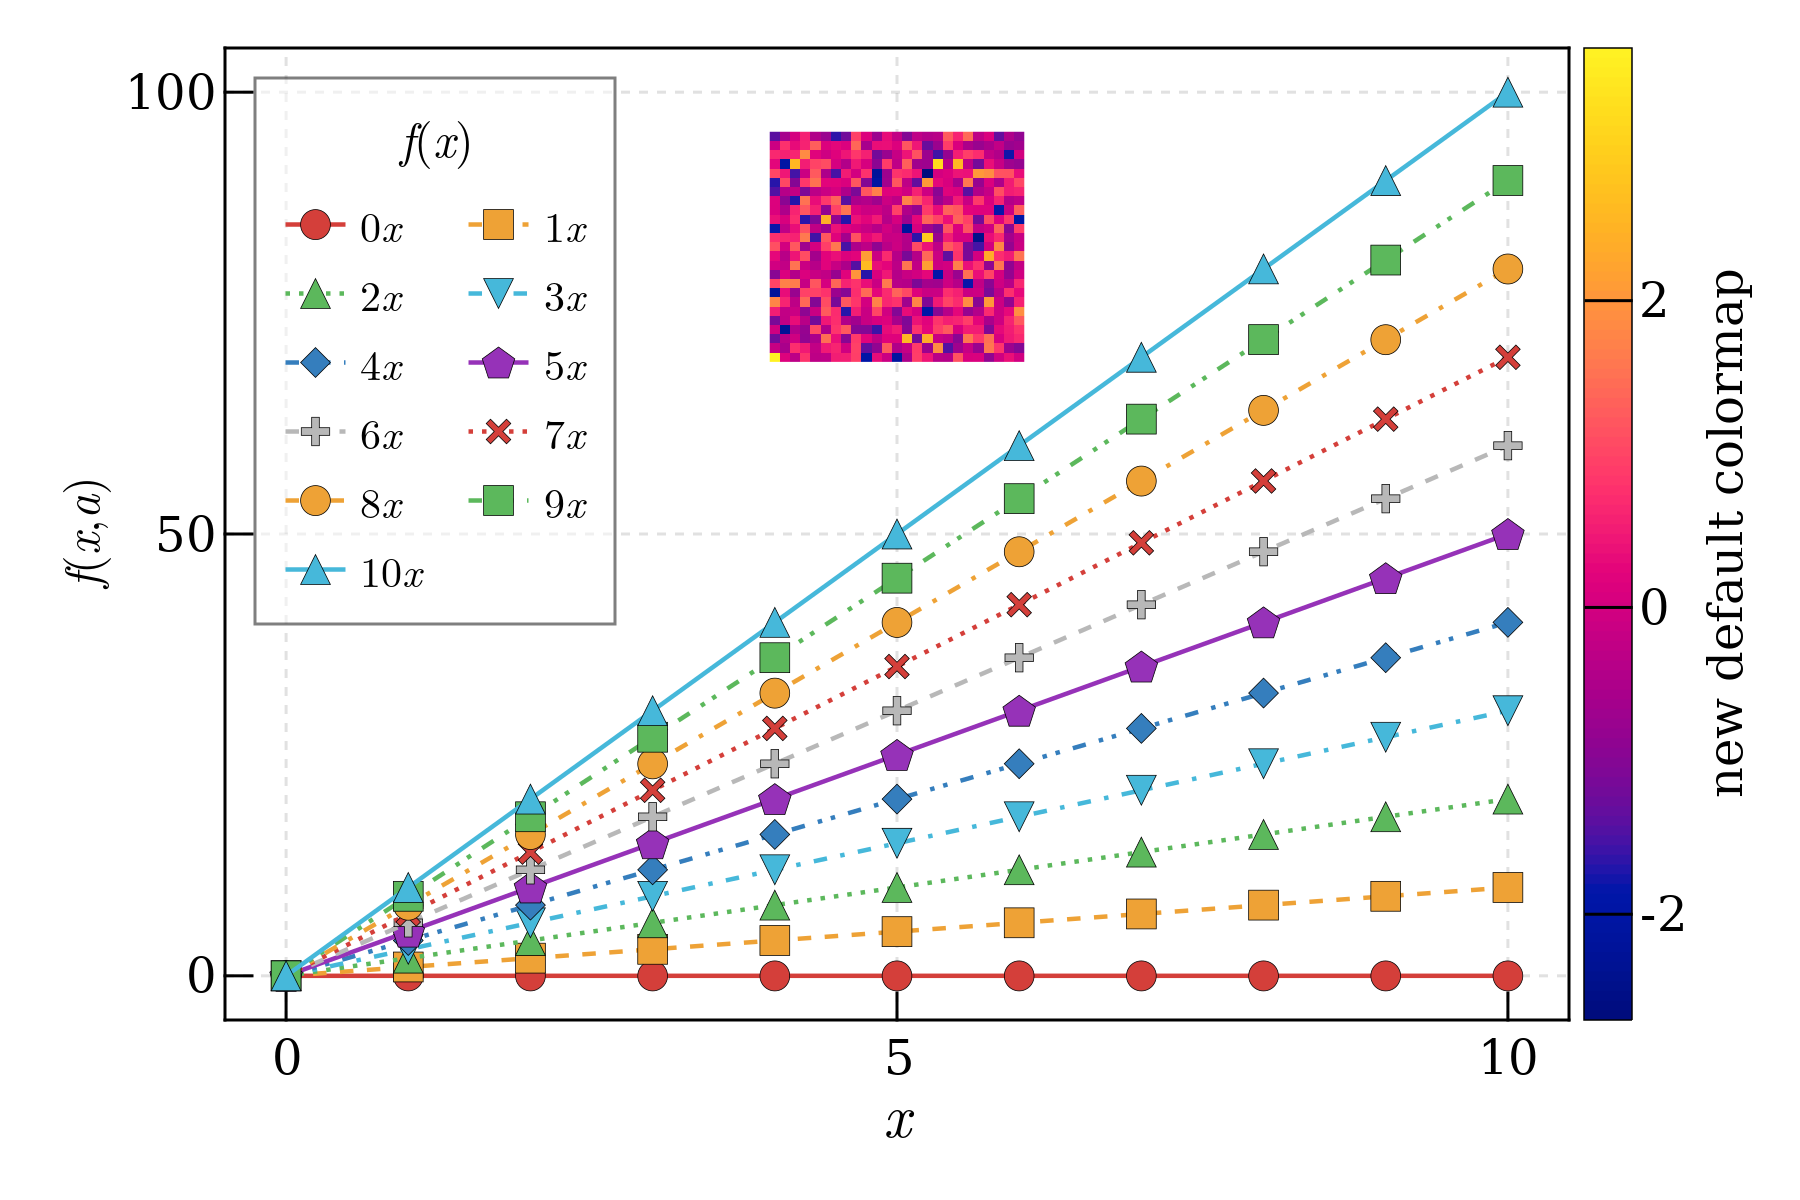
\includegraphics[width=0.6\textwidth,height=\textheight]{_build/im/custom_cycle.png}
\caption{Custom theme with new cycle and
colormap.}\label{fig:custom_cycle}
}
\end{figure}

At this point you should be able to have \textbf{complete control} over
your colors, line styles, markers and colormaps for your plots. Next, we
will dive into how to manage and control \textbf{layouts}.

\hypertarget{sec:makie_layouts}{%
\section{Layouts}\label{sec:makie_layouts}}

A complete \emph{canvas/layout} is defined by
\passthrough{\lstinline!Figure!}, which can be filled with content after
creation. We will start with a simple arrangement of one
\passthrough{\lstinline!Axis!}, one \passthrough{\lstinline!Legend!} and
one \passthrough{\lstinline!Colorbar!}. For this task we can think of
the canvas as an arrangement of \passthrough{\lstinline!rows!} and
\passthrough{\lstinline!columns!} in indexing a
\passthrough{\lstinline!Figure!} much like a regular
\passthrough{\lstinline!Array!}/\passthrough{\lstinline!Matrix!}. The
\passthrough{\lstinline!Axis!} content will be in \emph{row 1, column
1}, e.g.~\passthrough{\lstinline!fig[1, 1]!}, the
\passthrough{\lstinline!Colorbar!} in \emph{row 1, column 2}, namely
\passthrough{\lstinline!fig[1, 2]!}. And the
\passthrough{\lstinline!Legend!} in \emph{row 2} and across \emph{column
1 and 2}, namely \passthrough{\lstinline!fig[2, 1:2]!}.

\begin{lstlisting}[language=Julia]
function first_layout()
    seed!(123)
    x, y, z = randn(6), randn(6), randn(6)
    fig = Figure(resolution=(600, 400), backgroundcolor=:grey90)
    ax = Axis(fig[1, 1], backgroundcolor=:white)
    pltobj = scatter!(ax, x, y; color=z, label="scatters")
    lines!(ax, x, 1.1y; label="line")
    Legend(fig[2, 1:2], ax, "labels", orientation=:horizontal)
    Colorbar(fig[1, 2], pltobj, label="colorbar")
    fig
end
first_layout()
\end{lstlisting}

\begin{figure}
\hypertarget{fig:first_layout}{%
\centering
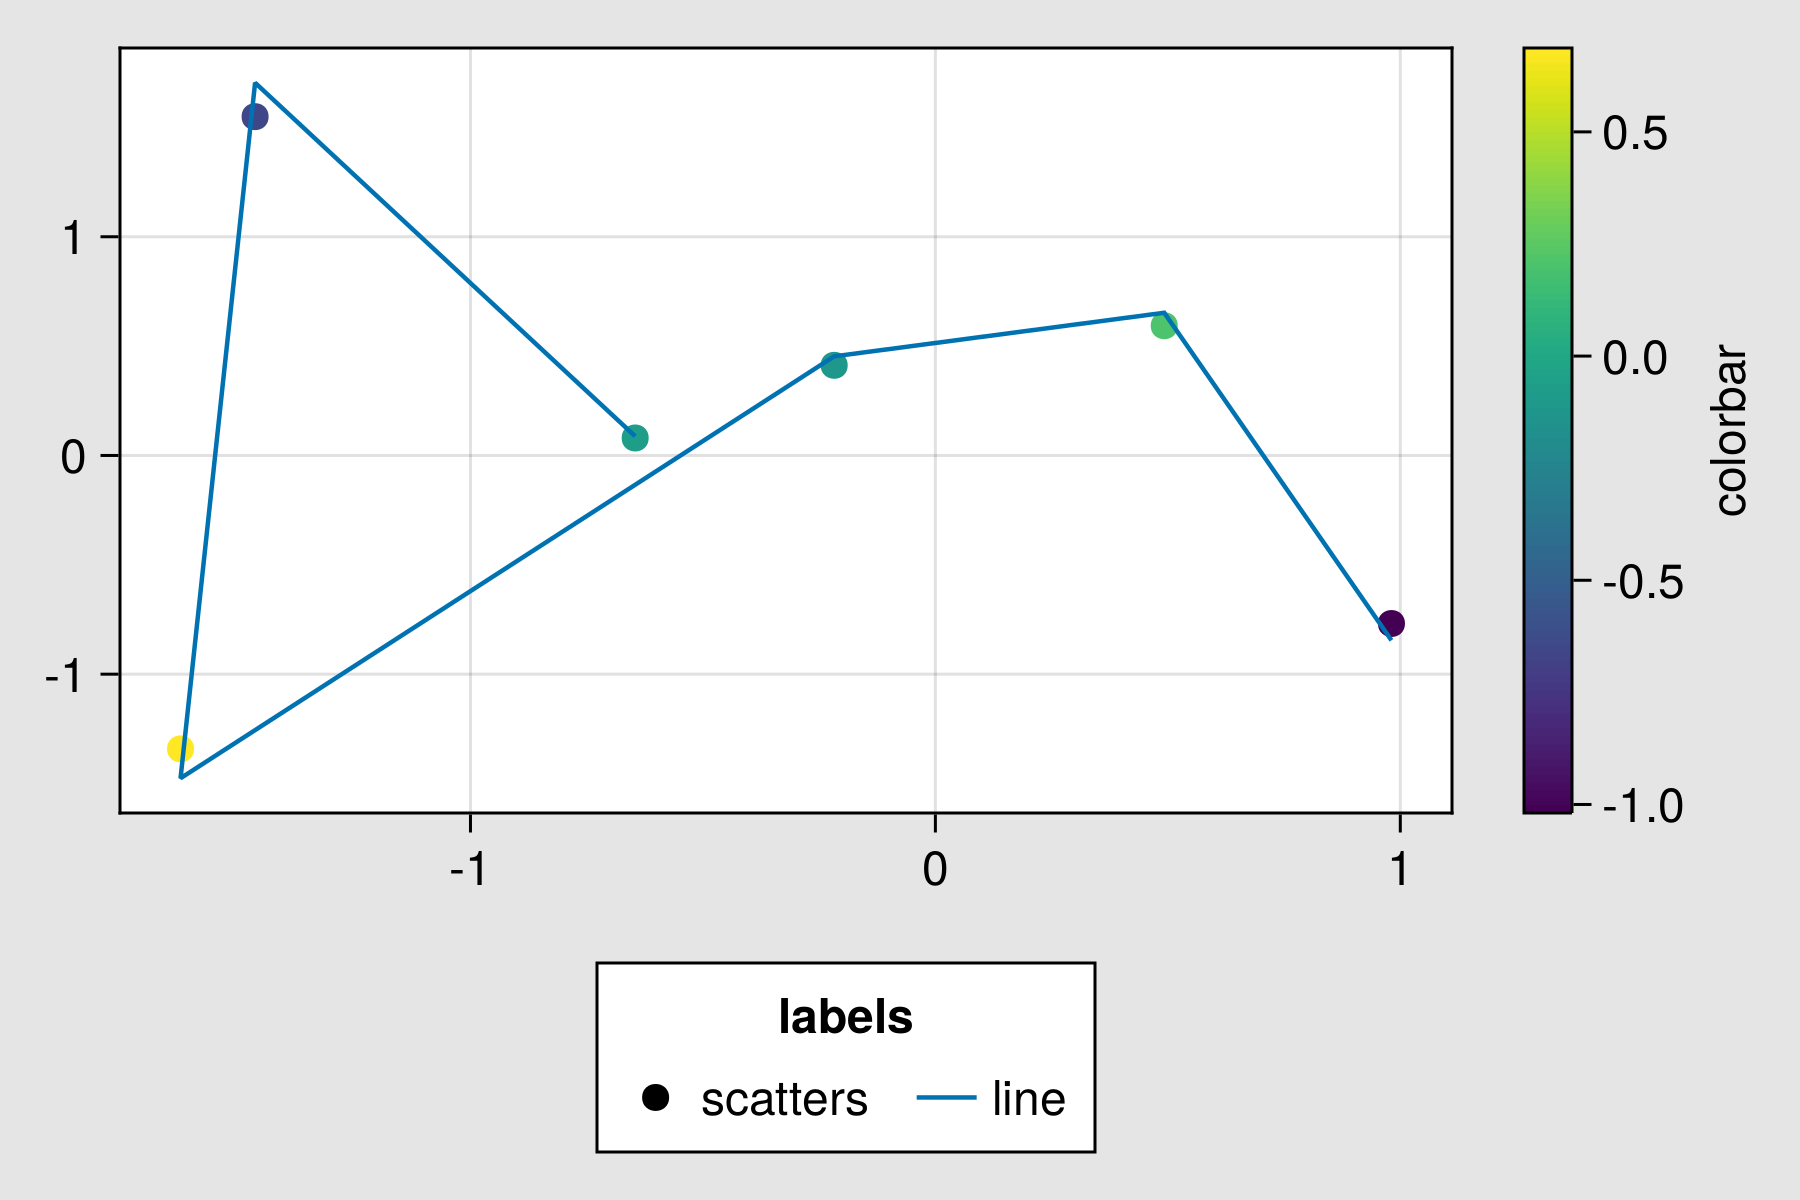
\includegraphics[width=0.6\textwidth,height=\textheight]{_build/im/JDS_first_layout_.png}
\caption{First Layout.}\label{fig:first_layout}
}
\end{figure}

This does look good already, but it could be better. We could fix
spacing problems using the following keywords and methods:

\begin{itemize}
\tightlist
\item
  \passthrough{\lstinline!figure\_padding=(left, right, bottom, top)!}
\item
  \passthrough{\lstinline!padding=(left, right, bottom, top)!}
\end{itemize}

Taking into account the actual size for a
\passthrough{\lstinline!Legend!} or \passthrough{\lstinline!Colorbar!}
is done by

\begin{quote}
\begin{itemize}
\tightlist
\item
  \passthrough{\lstinline!tellheight=true!} or
  \passthrough{\lstinline!false!}
\item
  \passthrough{\lstinline!tellwidth=true!} or
  \passthrough{\lstinline!false!}
\end{itemize}

\emph{Setting these to \passthrough{\lstinline!true!} will take into
account the actual size (height or width) for a
\passthrough{\lstinline!Legend!} or \passthrough{\lstinline!Colorbar!}}.
Consequently, things will be resized accordingly.
\end{quote}

The space between columns and rows is specified as

\begin{quote}
\begin{itemize}
\tightlist
\item
  \passthrough{\lstinline"colgap!(fig.layout, col, separation)"}
\item
  \passthrough{\lstinline"rowgap!(fig.layout, row, separation)"}
\end{itemize}

\emph{Column gap} (\passthrough{\lstinline"colgap!"}), if
\passthrough{\lstinline!col!} is given then the gap will be applied to
that specific column. \emph{Row gap}
(\passthrough{\lstinline"rowgap!"}), if \passthrough{\lstinline!row!} is
given then the gap will be applied to that specific row.
\end{quote}

Also, we will see how to put content into the \textbf{protrusions},
\emph{i.e.} the space reserved for \emph{title:
\passthrough{\lstinline!x!} and \passthrough{\lstinline!y!}; either
\passthrough{\lstinline!ticks!} or \passthrough{\lstinline!label!}}. We
do this by plotting into \passthrough{\lstinline!fig[i, j, protrusion]!}
where \emph{\passthrough{\lstinline!protrusion!}} can be
\passthrough{\lstinline!Left()!}, \passthrough{\lstinline!Right()!},
\passthrough{\lstinline!Bottom()!} and \passthrough{\lstinline!Top()!},
or for each corner \passthrough{\lstinline!TopLeft()!},
\passthrough{\lstinline!TopRight()!},
\passthrough{\lstinline!BottomRight()!},
\passthrough{\lstinline!BottomLeft()!}. See below how these options are
being used:

\begin{lstlisting}[language=Julia]
function first_layout_fixed()
    seed!(123)
    x, y, z = randn(6), randn(6), randn(6)
    fig = Figure(figure_padding=(0, 3, 5, 2), resolution=(600, 400),
        backgroundcolor=:grey90, font="CMU Serif")
    ax = Axis(fig[1, 1], xlabel=L"x", ylabel=L"y",
        title="Layout example", backgroundcolor=:white)
    pltobj = scatter!(ax, x, y; color=z, label="scatters")
    lines!(ax, x, 1.1y, label="line")
    Legend(fig[2, 1:2], ax, "Labels", orientation=:horizontal,
        tellheight=true, titleposition=:left)
    Colorbar(fig[1, 2], pltobj, label="colorbar")
    # additional aesthetics
    Box(fig[1, 1, Right()], color=(:slateblue1, 0.35))
    Label(fig[1, 1, Right()], "protrusion", textsize=18,
        rotation=pi / 2, padding=(3, 3, 3, 3))
    Label(fig[1, 1, TopLeft()], "(a)", textsize=18, padding=(0, 3, 8, 0))
    colgap!(fig.layout, 5)
    rowgap!(fig.layout, 5)
    fig
end
first_layout_fixed()
\end{lstlisting}

\begin{figure}
\hypertarget{fig:first_layout_fixed}{%
\centering
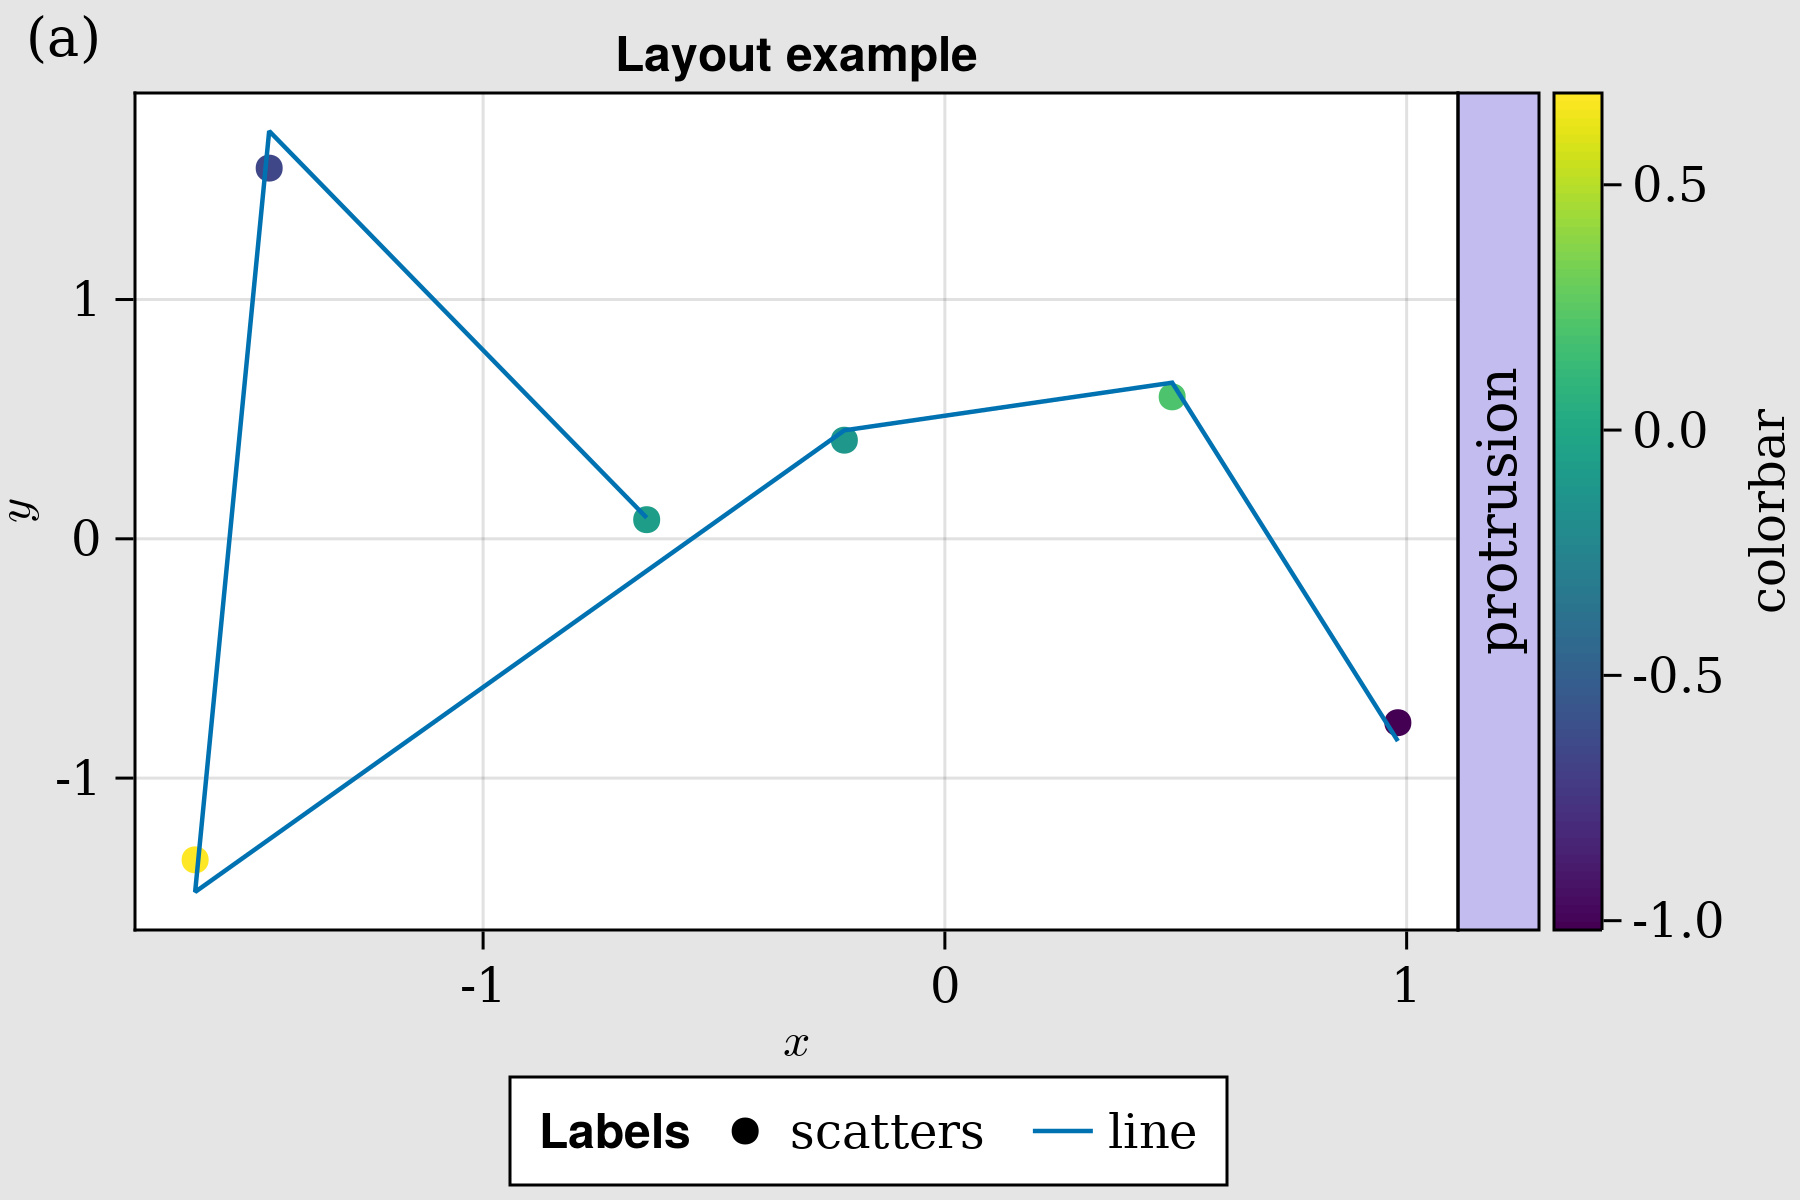
\includegraphics[width=0.6\textwidth,height=\textheight]{_build/im/JDS_first_layout_fixed_.png}
\caption{First Layout Fixed.}\label{fig:first_layout_fixed}
}
\end{figure}

Here, having the label \passthrough{\lstinline!(a)!} in the
\passthrough{\lstinline!TopLeft()!} is probably not necessary, this will
only make sense for more than one plot. For our next example let's keep
using the previous tools and some more to create a richer and complex
figure.

You can hide decorations and axis' spines with:

\begin{quote}
\begin{itemize}
\tightlist
\item
  \passthrough{\lstinline"hidedecorations!(ax; kwargs...)"}
\item
  \passthrough{\lstinline"hidexdecorations!(ax; kwargs...)"}
\item
  \passthrough{\lstinline"hideydecorations!(ax; kwargs...)"}
\item
  \passthrough{\lstinline"hidespines!(ax; kwargs...)"}
\end{itemize}
\end{quote}

Remember, we can always ask for help to see what kind of arguments we
can use, e.g.,

\begin{lstlisting}[language=Julia]
help(hidespines!)
\end{lstlisting}

\begin{lstlisting}[language=Output]
  hidespines!(la::Axis, spines::Symbol... = (:l, :r, :b, :t)...)

  Hide all specified axis spines. Hides all spines by default, otherwise
  choose with the symbols :l, :r, :b and :t.

  hidespines! has the following function signatures:

    (Vector, Vector)
    (Vector, Vector, Vector)
    (Matrix)

  Available attributes for Combined{Makie.MakieLayout.hidespines!} are:

  
\end{lstlisting}

Alternatively, for decorations

\begin{lstlisting}[language=Julia]
help(hidedecorations!)
\end{lstlisting}

\begin{lstlisting}[language=Output]
  hidedecorations!(la::Axis)

  Hide decorations of both x and y-axis: label, ticklabels, ticks and grid.

  hidedecorations! has the following function signatures:

    (Vector, Vector)
    (Vector, Vector, Vector)
    (Matrix)

  Available attributes for Combined{Makie.MakieLayout.hidedecorations!} are:

  
\end{lstlisting}

For elements that \textbf{you don't want to hide}, just pass them with
\passthrough{\lstinline!false!},
i.e.~\passthrough{\lstinline"hideydecorations!(ax; ticks=false, grid=false)"}.

Synchronizing your \passthrough{\lstinline!Axis!} is done via:

\begin{quote}
\begin{itemize}
\tightlist
\item
  \passthrough{\lstinline"linkaxes!"},
  \passthrough{\lstinline"linkyaxes!"} and
  \passthrough{\lstinline"linkxaxes!"}
\end{itemize}

This could be useful when shared axis are desired. Another way of
getting shared axis will be by setting
\passthrough{\lstinline"limits!"}.
\end{quote}

Setting \passthrough{\lstinline!limits!} at once or independently for
each axis is done by calling

\begin{quote}
\begin{itemize}
\tightlist
\item
  \passthrough{\lstinline"limits!(ax; l, r, b, t)"}, where
  \passthrough{\lstinline!l!} is left, \passthrough{\lstinline!r!}
  right, \passthrough{\lstinline!b!} bottom, and
  \passthrough{\lstinline!t!} top.
\end{itemize}

You can also do \passthrough{\lstinline"ylims!(low, high)"} or
\passthrough{\lstinline"xlims!(low, high)"}, and even open ones by doing
\passthrough{\lstinline"ylims!(low=0)"} or
\passthrough{\lstinline"xlims!(high=1)"}.
\end{quote}

Now, the example:

\begin{lstlisting}[language=Julia]
function complex_layout_double_axis()
    seed!(123)
    x = LinRange(0, 1, 10)
    y = LinRange(0, 1, 10)
    z = rand(10, 10)
    fig = Figure(resolution=(600, 400), font="CMU Serif", backgroundcolor=:grey90)
    ax1 = Axis(fig, xlabel=L"x", ylabel=L"y")
    ax2 = Axis(fig, xlabel=L"x")
    heatmap!(ax1, x, y, z; colorrange=(0, 1))
    series!(ax2, abs.(z[1:4, :]); labels=["lab $i" for i = 1:4], color=:Set1_4)
    hm = scatter!(10x, y; color=z[1, :], label="dots", colorrange=(0, 1))
    hideydecorations!(ax2, ticks=false, grid=false)
    linkyaxes!(ax1, ax2)
    #layout
    fig[1, 1] = ax1
    fig[1, 2] = ax2
    Label(fig[1, 1, TopLeft()], "(a)", textsize=18, padding=(0, 6, 8, 0))
    Label(fig[1, 2, TopLeft()], "(b)", textsize=18, padding=(0, 6, 8, 0))
    Colorbar(fig[2, 1:2], hm, label="colorbar", vertical=false, flipaxis=false)
    Legend(fig[1, 3], ax2, "Legend")
    colgap!(fig.layout, 5)
    rowgap!(fig.layout, 5)
    fig
end
complex_layout_double_axis()
\end{lstlisting}

\begin{figure}
\hypertarget{fig:complex_layout_double_axis}{%
\centering
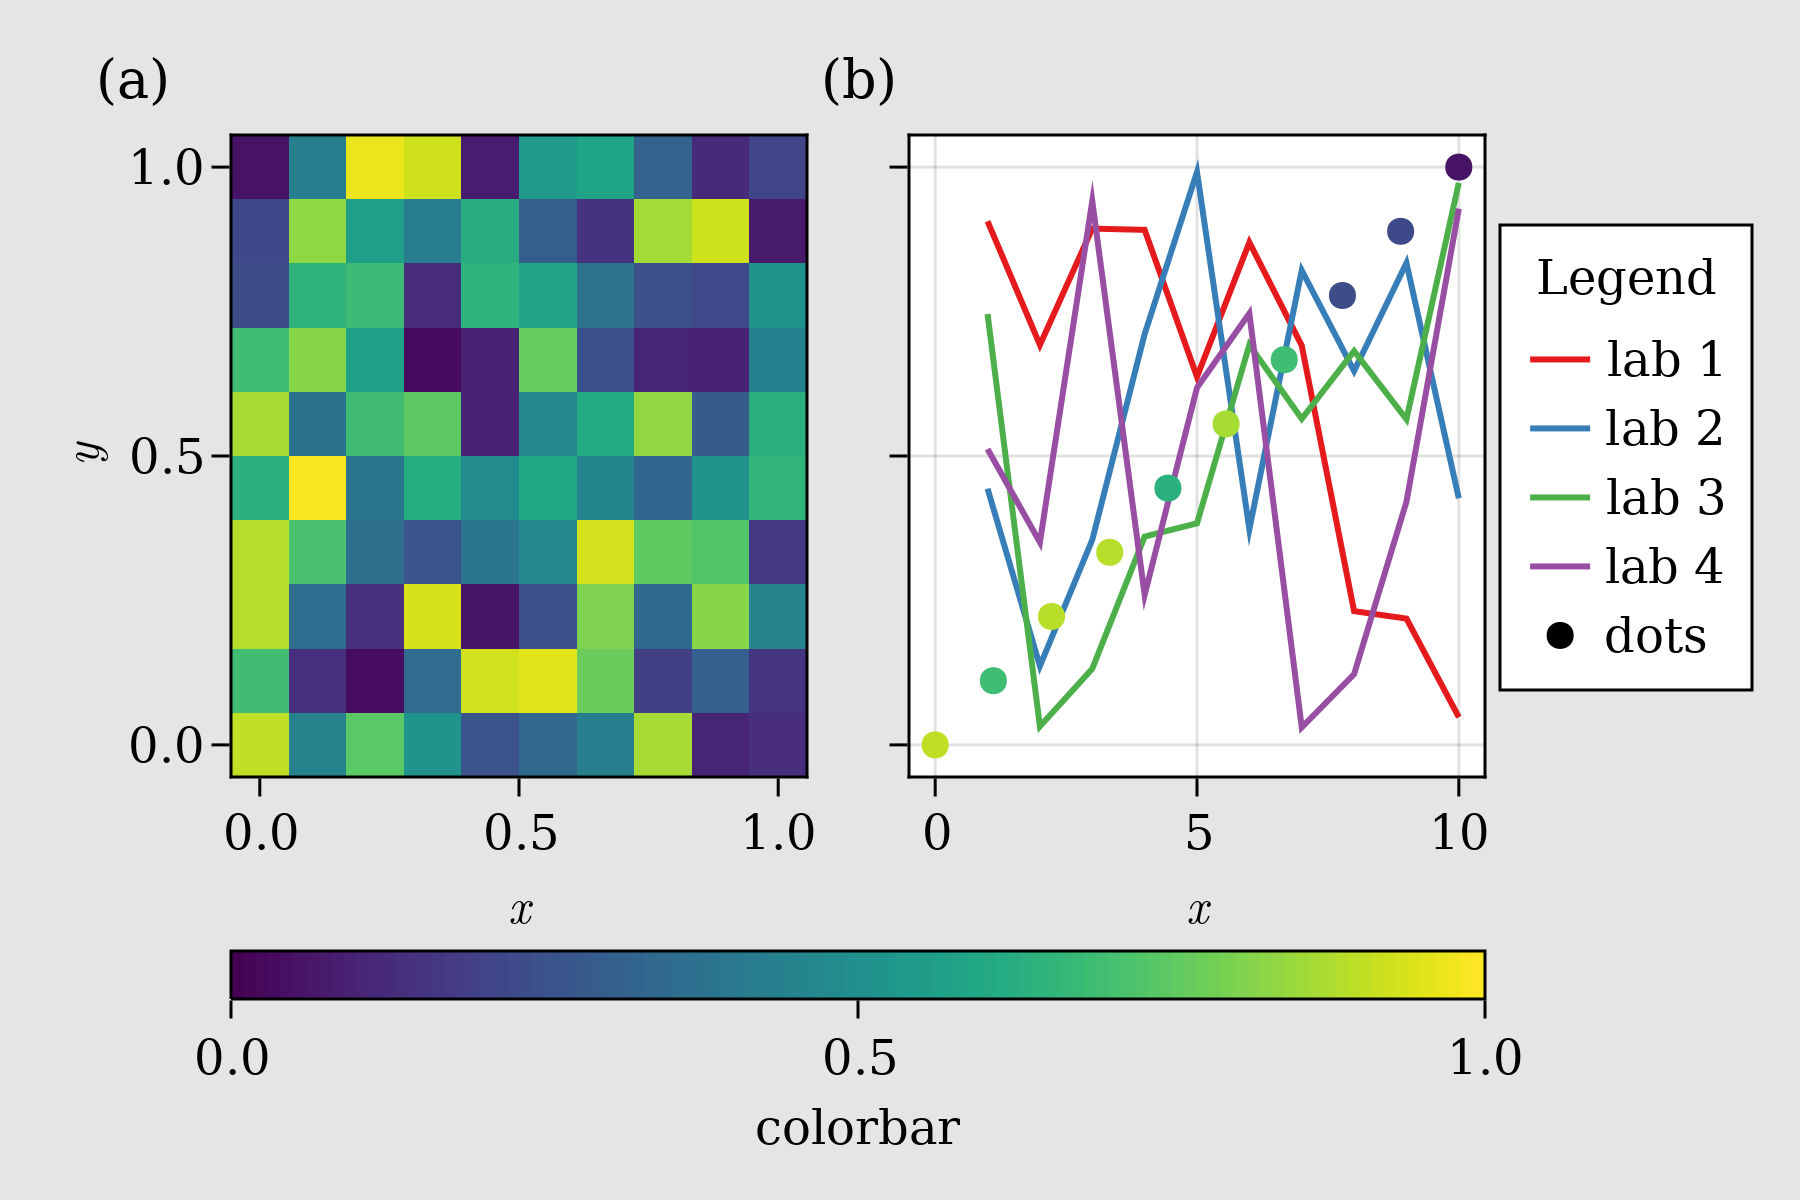
\includegraphics[width=0.6\textwidth,height=\textheight]{_build/im/JDS_complex_layout_double_axis_.png}
\caption{Complex layout double
axis.}\label{fig:complex_layout_double_axis}
}
\end{figure}

So, now our \passthrough{\lstinline!Colorbar!} needs to be horizontal
and the bar ticks need to be in the lower part. This is done by setting
\passthrough{\lstinline!vertical=false!} and
\passthrough{\lstinline!flipaxis=false!}. Additionally, note that we can
call many \passthrough{\lstinline!Axis!} into
\passthrough{\lstinline!fig!}, or even
\passthrough{\lstinline!Colorbar!}'s and
\passthrough{\lstinline!Legend!}'s, and then afterwards build the
layout.

Another common layout is a grid of squares for heatmaps:

\begin{lstlisting}[language=Julia]
function squares_layout()
    seed!(123)
    letters = reshape(collect('a':'d'), (2, 2))
    fig = Figure(resolution=(600, 400), fontsize=14, font="CMU Serif",
        backgroundcolor=:grey90)
    axs = [Axis(fig[i, j], aspect=DataAspect()) for i = 1:2, j = 1:2]
    hms = [heatmap!(axs[i, j], randn(10, 10), colorrange=(-2, 2))
           for i = 1:2, j = 1:2]
    Colorbar(fig[1:2, 3], hms[1], label="colorbar")
    [Label(fig[i, j, TopLeft()], "($(letters[i, j]))", textsize=16,
        padding=(-2, 0, -20, 0)) for i = 1:2, j = 1:2]
    colgap!(fig.layout, 5)
    rowgap!(fig.layout, 5)
    fig
end
squares_layout()
\end{lstlisting}

\begin{figure}
\hypertarget{fig:squares_layout}{%
\centering
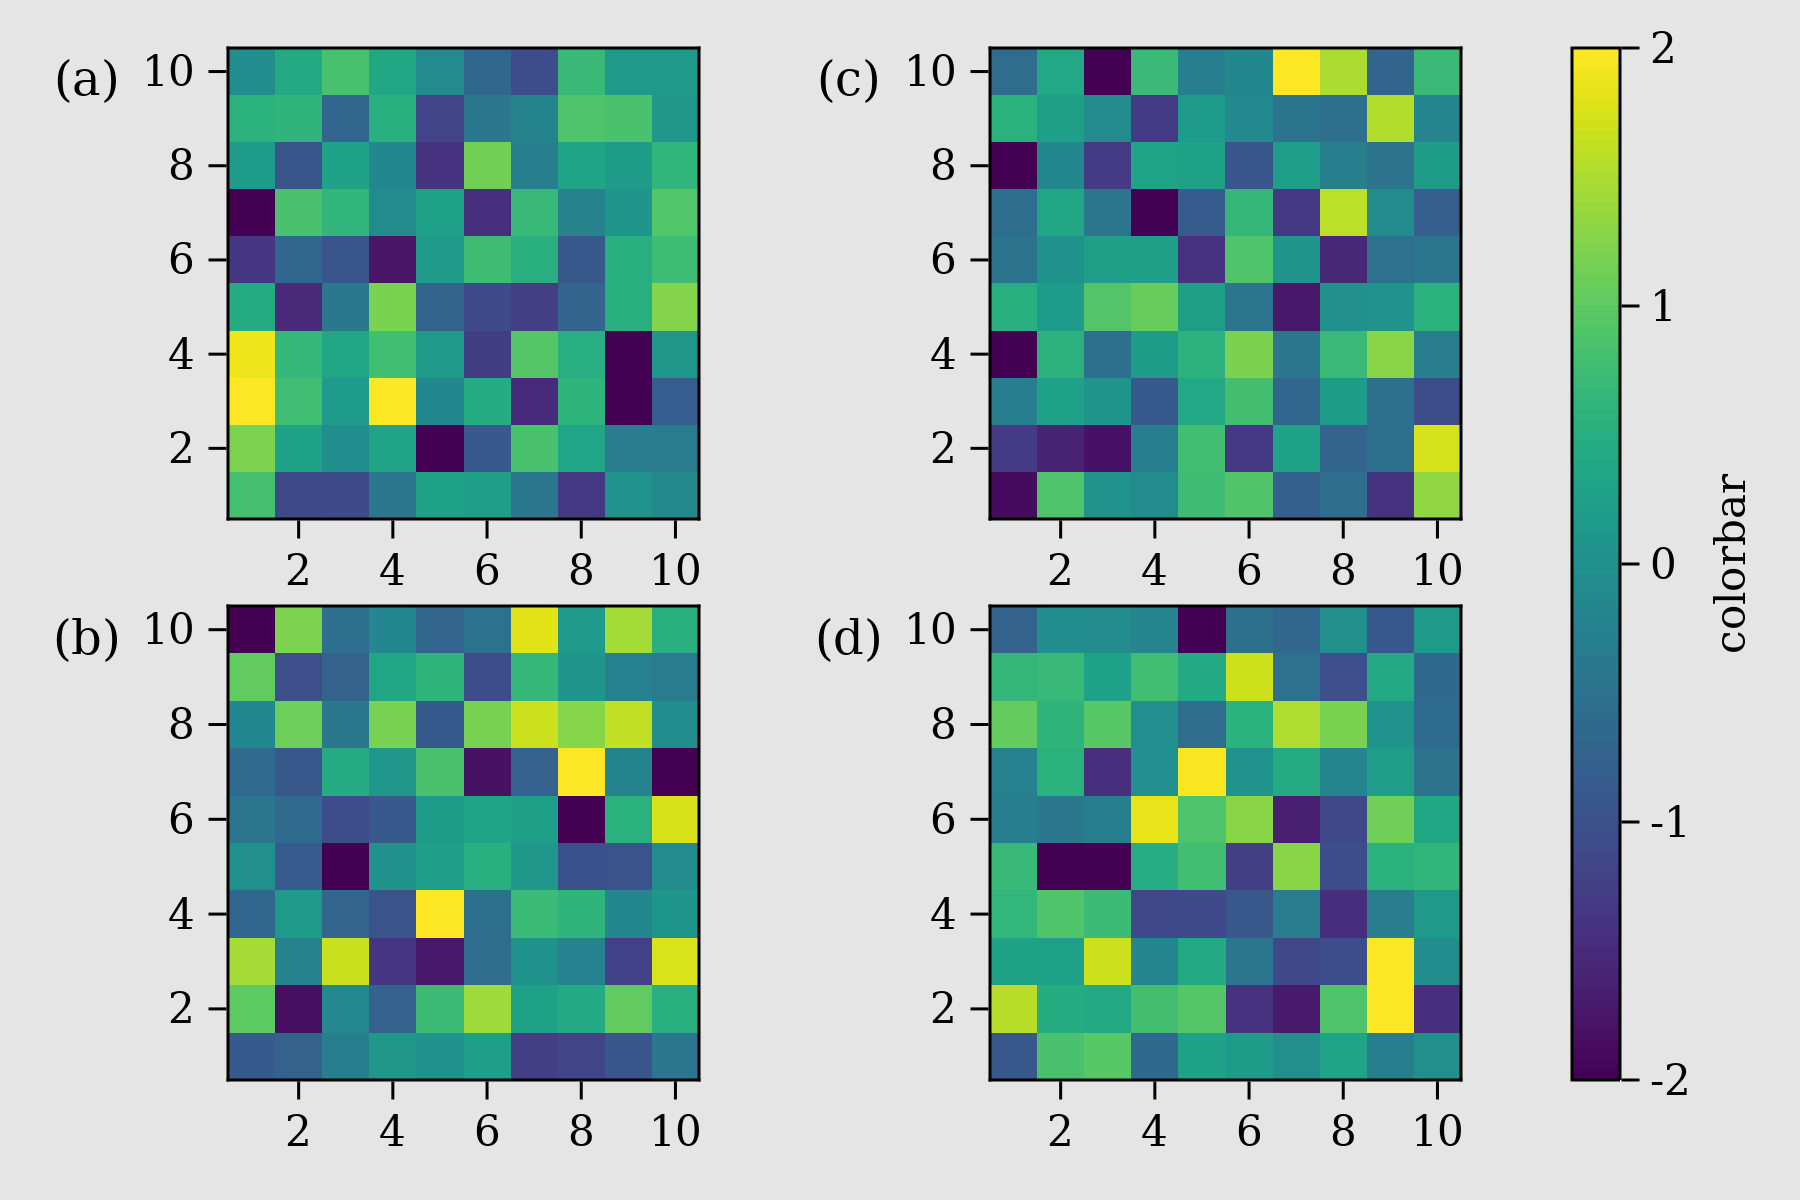
\includegraphics[width=0.6\textwidth,height=\textheight]{_build/im/JDS_squares_layout_.png}
\caption{Squares layout.}\label{fig:squares_layout}
}
\end{figure}

where all labels are in the \textbf{protrusions} and each
\passthrough{\lstinline!Axis!} has an
\passthrough{\lstinline!AspectData()!} ratio. The
\passthrough{\lstinline!Colorbar!} is located in the third column and
expands from row 1 up to row 2.

The next case uses the so called \passthrough{\lstinline!Mixed()!}
\textbf{alignmode}, which is especially useful when dealing with large
empty spaces between \passthrough{\lstinline!Axis!} due to long ticks.
Also, the \passthrough{\lstinline!Dates!} module from Julia's standard
library will be needed for this example.

\begin{lstlisting}
using Dates
\end{lstlisting}

\begin{lstlisting}[language=Julia]
function mixed_mode_layout()
    seed!(123)
    longlabels = ["$(today() - Day(1))", "$(today())", "$(today() + Day(1))"]
    fig = Figure(resolution = (600, 400), fontsize = 12,
        backgroundcolor = :grey90, font = "CMU Serif")
    ax1 = Axis(fig[1, 1], xlabel = "x", alignmode = Mixed(bottom = 0))
    ax2 = Axis(fig[1, 2], xticklabelrotation = pi / 2, alignmode = Mixed(bottom = 0),
        xticks = ([1, 5, 10], longlabels))
    ax3 = Axis(fig[2, 1:2])
    ax4 = Axis(fig[3, 1:2])
    axs = [ax1, ax2, ax3, ax4]
    [lines!(ax, 1:10, rand(10)) for ax in axs]
    hidexdecorations!(ax3; ticks = false, grid = false)
    Box(fig[2:3, 1:2, Right()], color = (:slateblue1, 0.35))
    Label(fig[2:3, 1:2, Right()], "protrusion", rotation = pi / 2, textsize = 14,
        padding = (3, 3, 3, 3))
    Label(fig[1, 1:2, Top()], "Mixed alignmode", textsize = 16,
        padding = (0, 0, 15, 0))
    colsize!(fig.layout, 1, Auto(2))
    rowsize!(fig.layout, 2, Auto(0.5))
    rowsize!(fig.layout, 3, Auto(0.5))
    rowgap!(fig.layout, 1, 15)
    rowgap!(fig.layout, 2, 0)
    colgap!(fig.layout, 5)
    fig
end
mixed_mode_layout()
\end{lstlisting}

\begin{figure}
\hypertarget{fig:mixed_mode_layout}{%
\centering
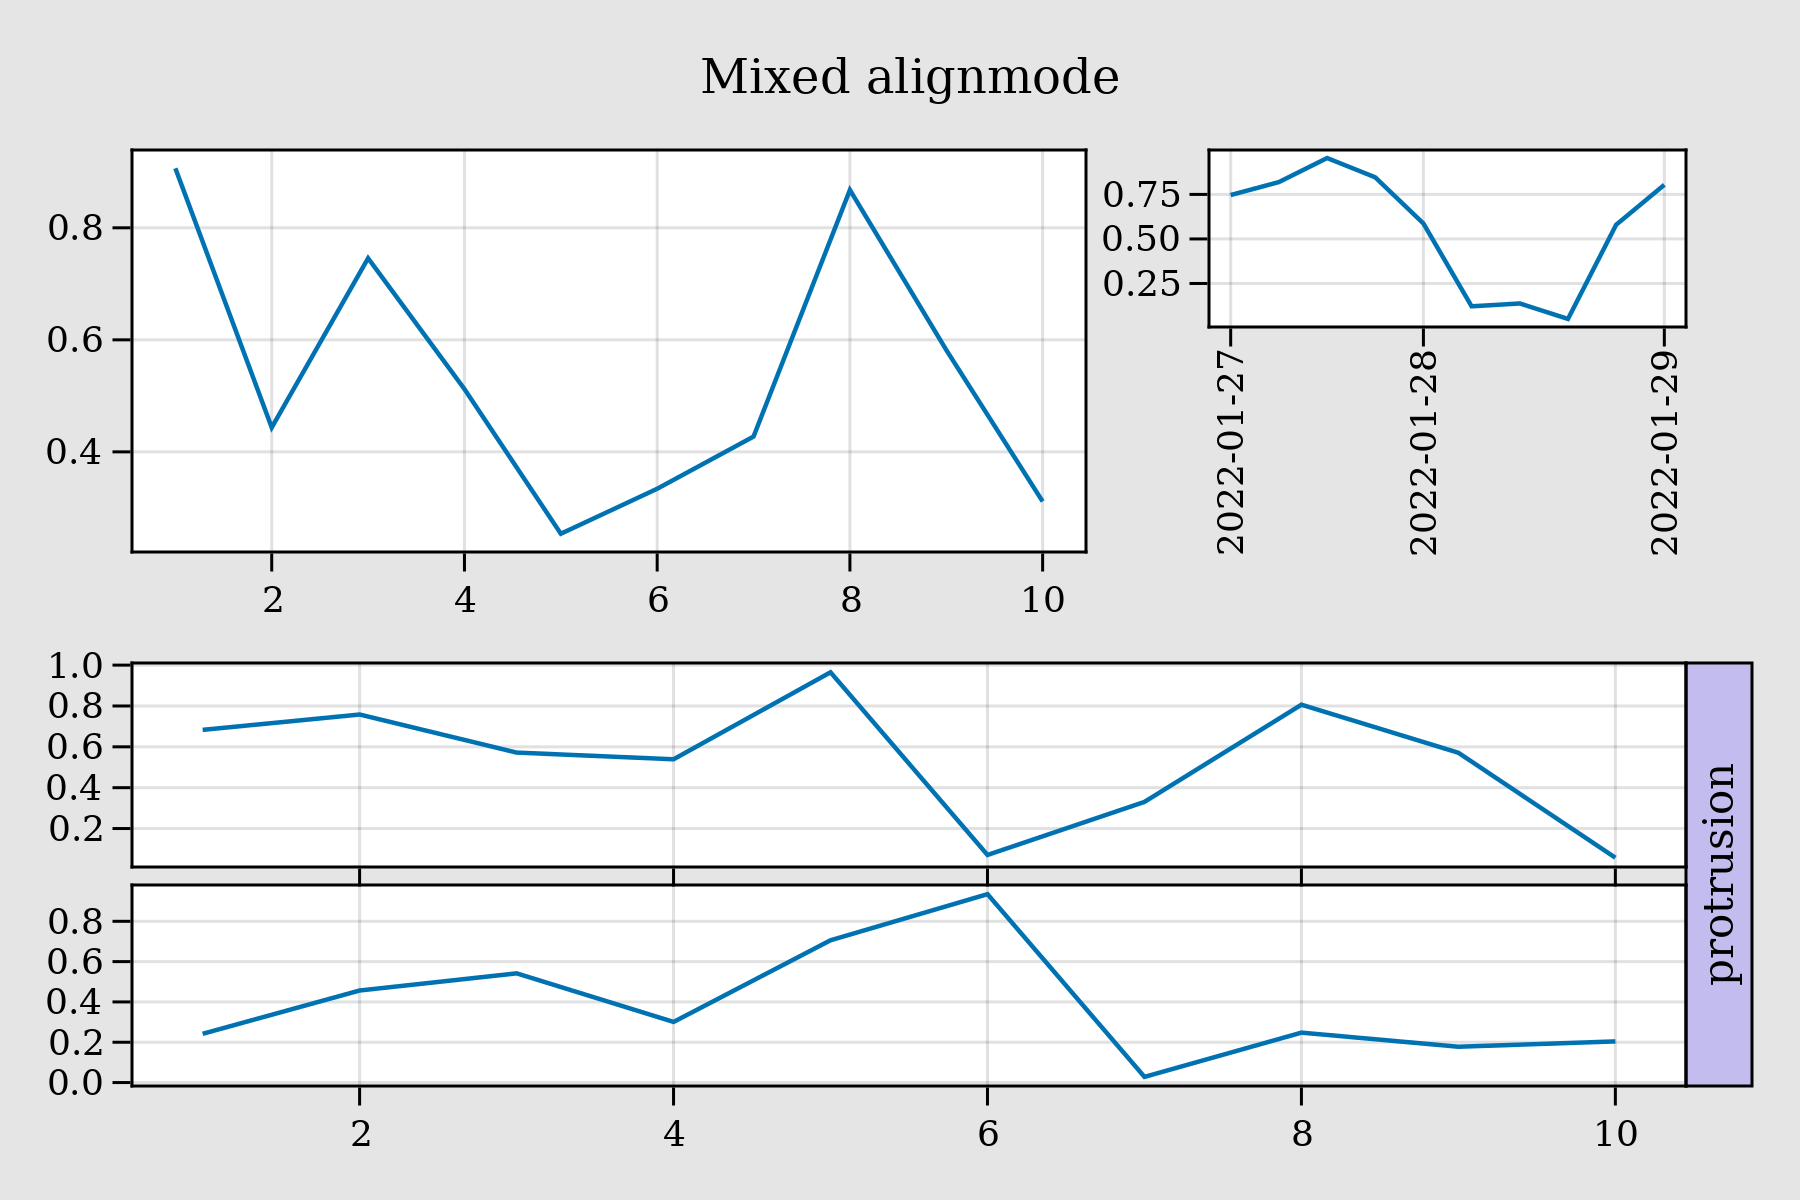
\includegraphics[width=0.6\textwidth,height=\textheight]{_build/im/JDS_mixed_mode_layout_.png}
\caption{Mixed mode layout.}\label{fig:mixed_mode_layout}
}
\end{figure}

Here, the argument \passthrough{\lstinline!alignmode=Mixed(bottom=0)!}
is shifting the bounding box to the bottom, so that this will align with
the panel on the left filling the space.

Also, see how \passthrough{\lstinline"colsize!"} and
\passthrough{\lstinline"rowsize!"} are being used for different columns
and rows. You could also put a number instead of
\passthrough{\lstinline!Auto()!} but then everything will be fixed. And,
additionally, one could also give a \passthrough{\lstinline!height!} or
\passthrough{\lstinline!width!} when defining the
\passthrough{\lstinline!Axis!}, as in
\passthrough{\lstinline!Axis(fig, height=50)!} which will be fixed as
well.

\hypertarget{nested-axis-subplots}{%
\subsection{\texorpdfstring{Nested \texttt{Axis}
(\emph{subplots})}{Nested Axis (subplots)}}\label{nested-axis-subplots}}

It is also possible to define a set of \passthrough{\lstinline!Axis!}
(\emph{subplots}) explicitly, and use it to build a main figure with
several rows and columns. For instance, the following is a
``complicated'' arrangement of \passthrough{\lstinline!Axis!}:

\begin{lstlisting}[language=Julia]
function nested_sub_plot!(fig)
    color = rand(RGBf)
    ax1 = Axis(fig[1, 1], backgroundcolor=(color, 0.25))
    ax2 = Axis(fig[1, 2], backgroundcolor=(color, 0.25))
    ax3 = Axis(fig[2, 1:2], backgroundcolor=(color, 0.25))
    ax4 = Axis(fig[1:2, 3], backgroundcolor=(color, 0.25))
    return (ax1, ax2, ax3, ax4)
end
\end{lstlisting}

which, when used to build a more complex figure by doing several calls,
we obtain:

\begin{lstlisting}[language=Julia]
function main_figure()
    fig = Figure()
    Axis(fig[1, 1])
    nested_sub_plot!(fig[1, 2])
    nested_sub_plot!(fig[1, 3])
    nested_sub_plot!(fig[2, 1:3])
    fig
end
main_figure()
\end{lstlisting}

\begin{figure}
\hypertarget{fig:main_figure}{%
\centering
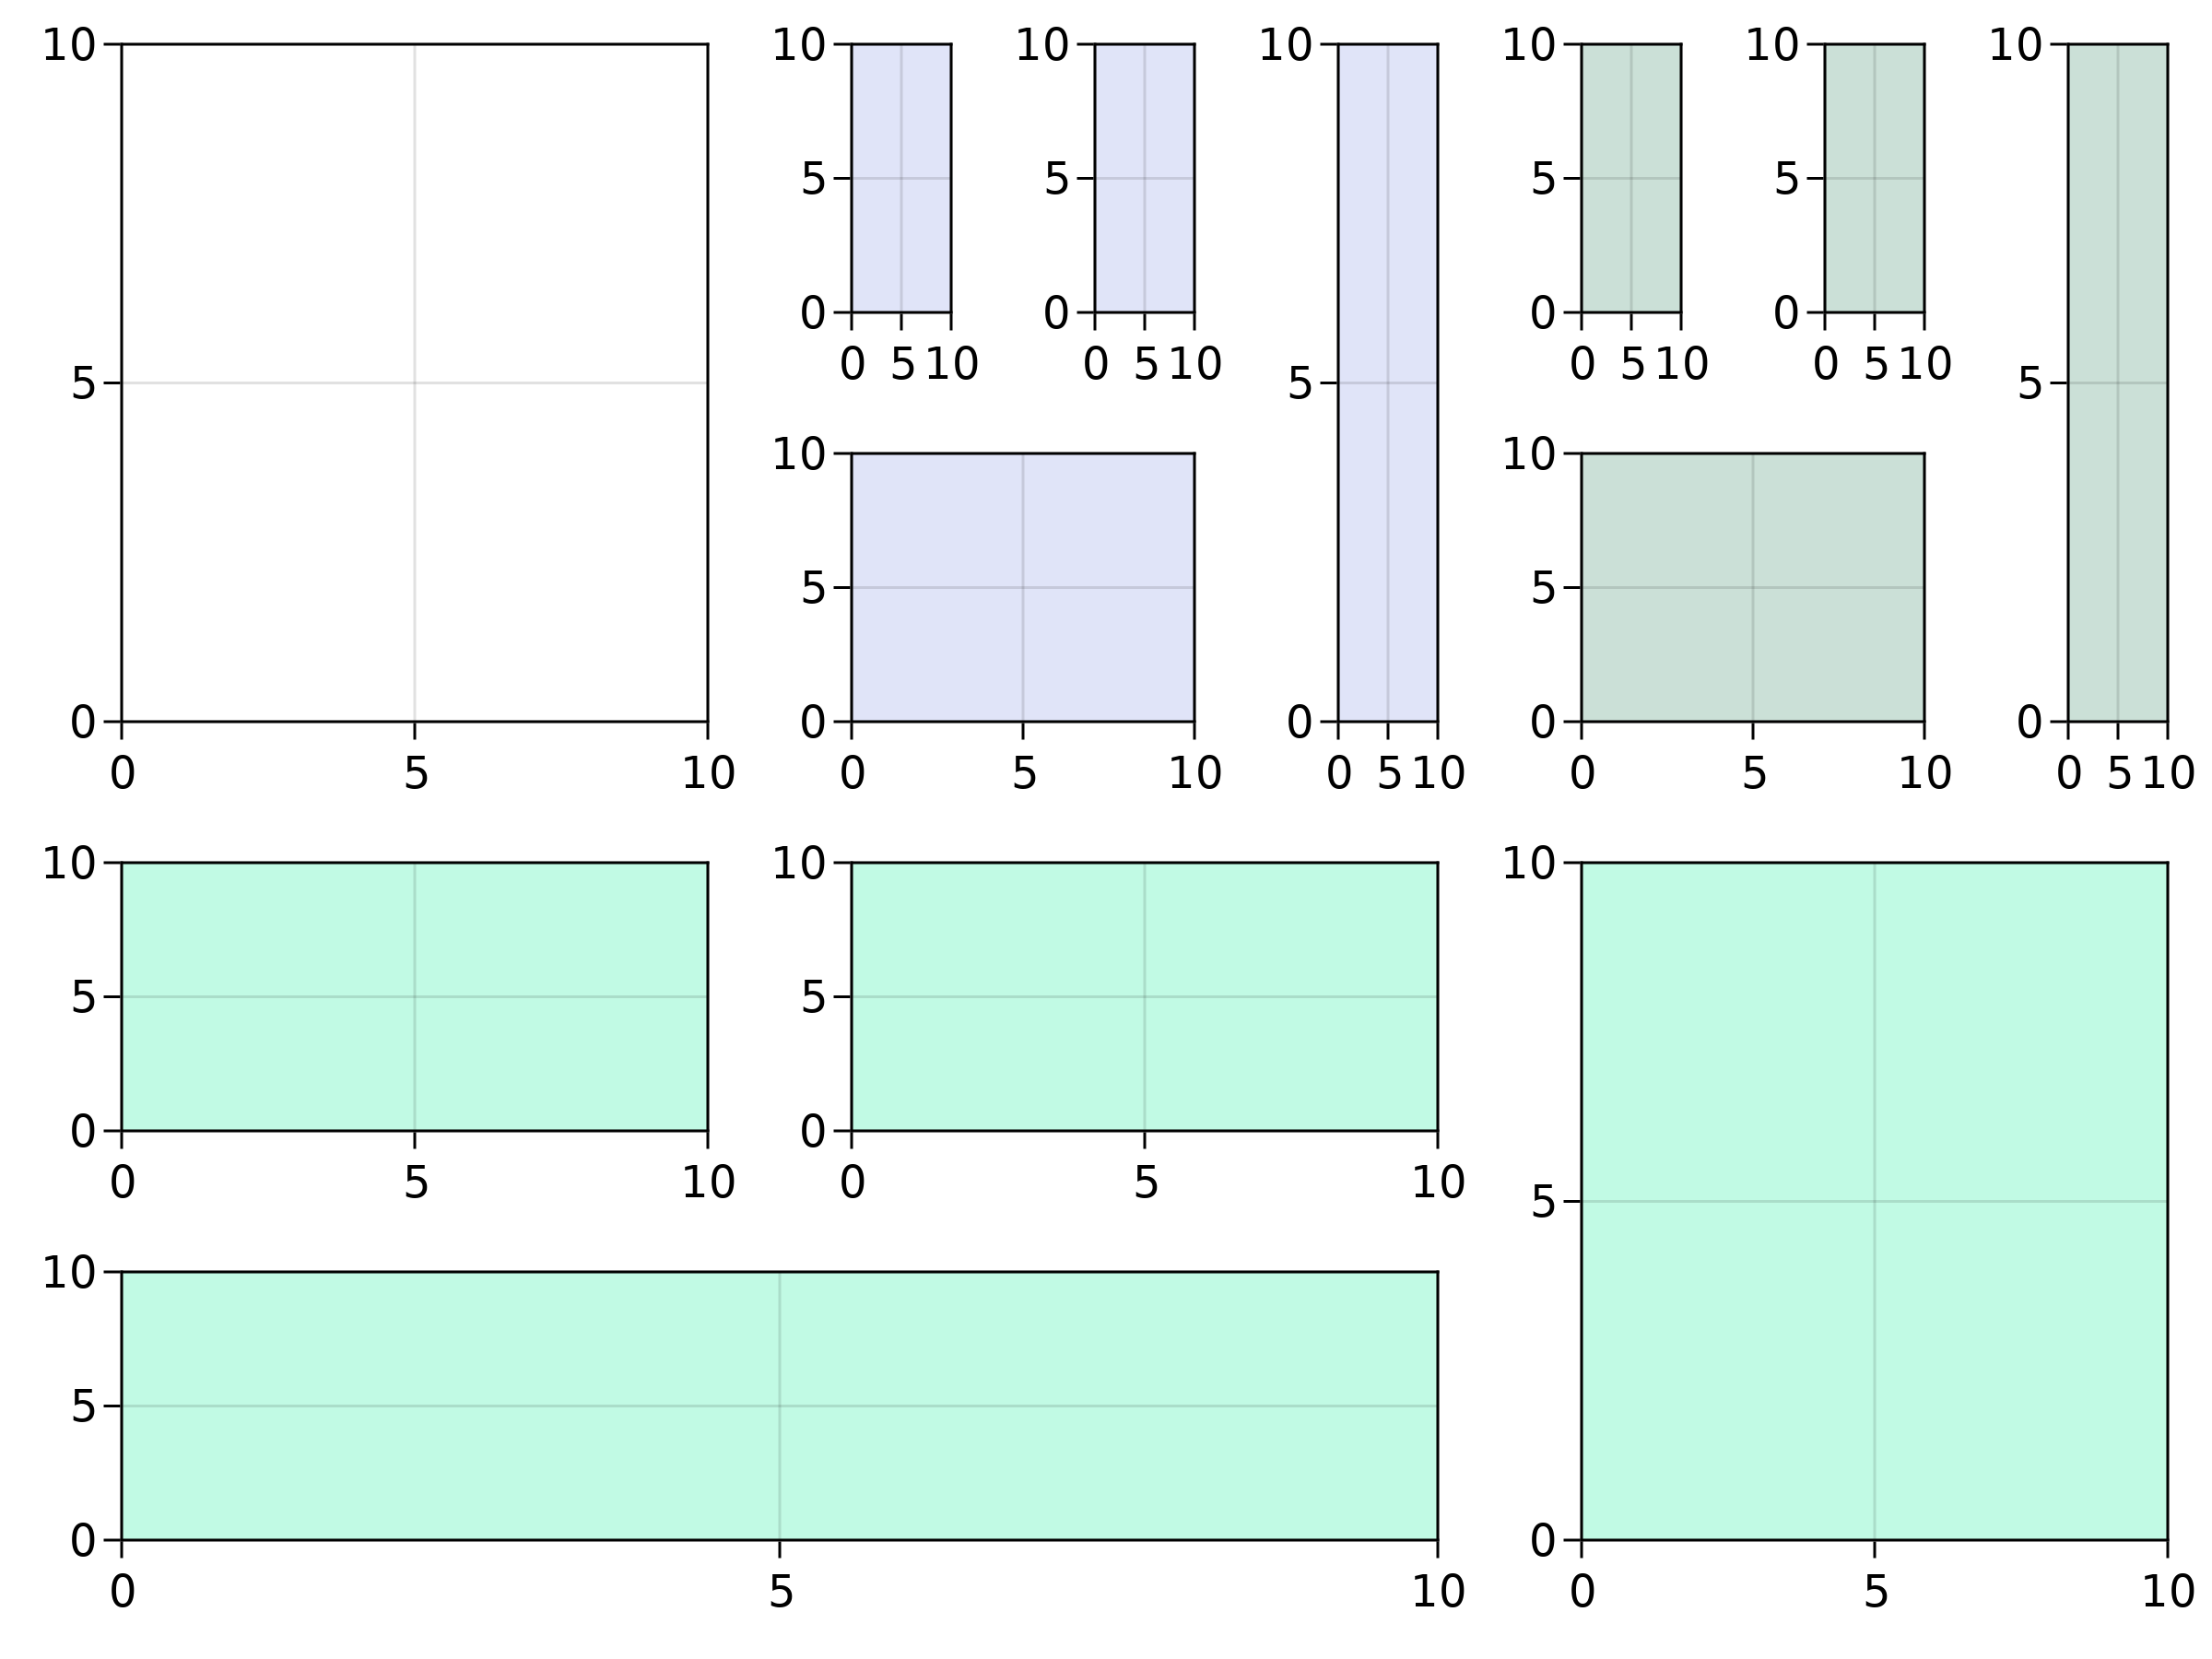
\includegraphics[width=0.6\textwidth,height=\textheight]{_build/im/JDS_main_figure_.png}
\caption{Main figure.}\label{fig:main_figure}
}
\end{figure}

Note that different subplot functions can be called here. Also, each
\passthrough{\lstinline!Axis!} here is an independent part of
\passthrough{\lstinline!Figure!}. So that, if you need to do some
\passthrough{\lstinline"rowgap!"}'s or
\passthrough{\lstinline"colsize!"}'s operations, you will need to do it
in each one of them independently or to all of them together.

For grouped \passthrough{\lstinline!Axis!} (\emph{subplots}) we can use
\passthrough{\lstinline!GridLayout()!} which, then, could be used to
compose a more complicated \passthrough{\lstinline!Figure!}.

\hypertarget{nested-gridlayout}{%
\subsection{Nested GridLayout}\label{nested-gridlayout}}

By using \passthrough{\lstinline!GridLayout()!} we can group subplots,
allowing more freedom to build complex figures. Here, using our previous
\passthrough{\lstinline"nested\_sub\_plot!"} we define three sub-groups
and one normal \passthrough{\lstinline!Axis!}:

\begin{lstlisting}[language=Julia]
function nested_Grid_Layouts()
    fig = Figure(backgroundcolor=RGBf(0.96, 0.96, 0.96))
    ga = fig[1, 1] = GridLayout()
    gb = fig[1, 2] = GridLayout()
    gc = fig[1, 3] = GridLayout()
    gd = fig[2, 1:3] = GridLayout()
    gA = Axis(ga[1, 1])
    nested_sub_plot!(gb)
    axsc = nested_sub_plot!(gc)
    nested_sub_plot!(gd)
    hidedecorations!.(axsc, grid=false, ticks=false)
    colgap!(gc, 5)
    rowgap!(gc, 5)
    rowsize!(fig.layout, 2, Auto(0.5))
    colsize!(fig.layout, 1, Auto(0.5))
    fig
end
nested_Grid_Layouts()
\end{lstlisting}

\begin{figure}
\hypertarget{fig:nested_Grid_Layouts}{%
\centering
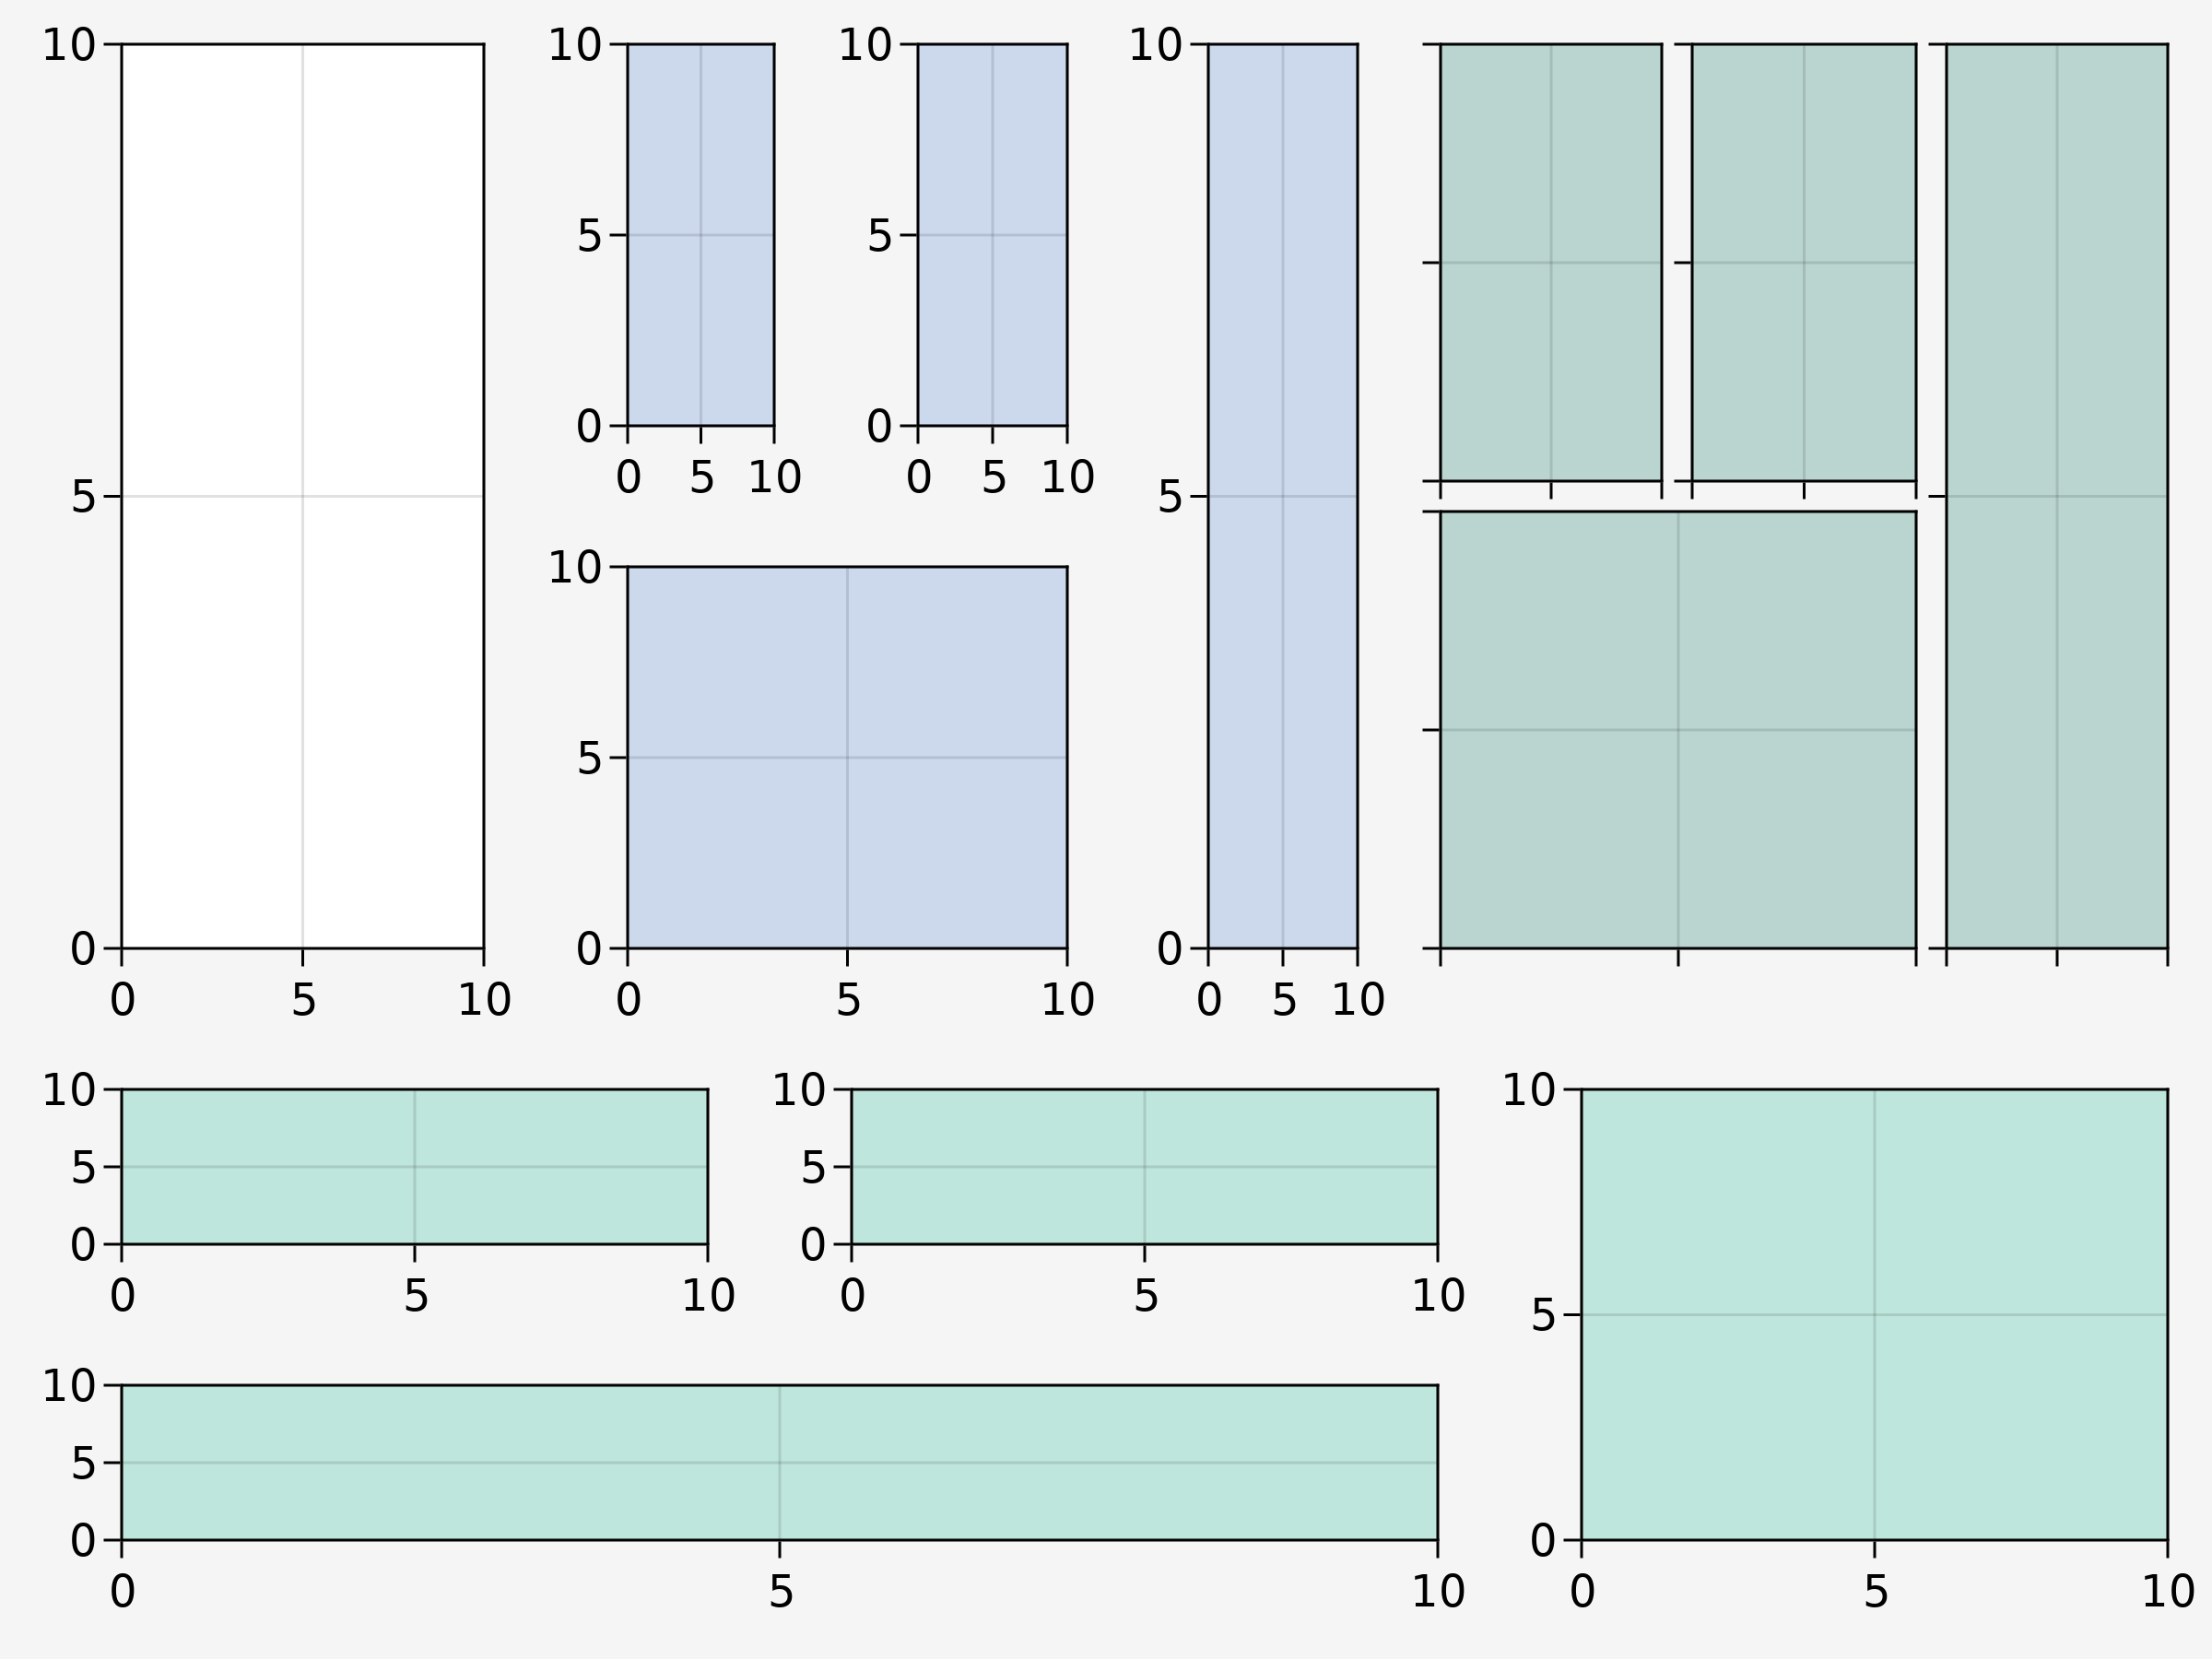
\includegraphics[width=0.6\textwidth,height=\textheight]{_build/im/JDS_nested_Grid_Layouts_.png}
\caption{Nested Grid Layouts.}\label{fig:nested_Grid_Layouts}
}
\end{figure}

Now, using \passthrough{\lstinline"rowgap!"} or
\passthrough{\lstinline"colsize!"} over each group is possible and
\passthrough{\lstinline"rowsize!, colsize!"} can also be applied to the
set of \passthrough{\lstinline!GridLayout()!}s.

\hypertarget{inset-plots}{%
\subsection{Inset plots}\label{inset-plots}}

Currently, doing \passthrough{\lstinline!inset!} plots is a little bit
tricky. Here, we show two possible ways of doing it by initially
defining auxiliary functions. The first one is by doing a
\passthrough{\lstinline!BBox!}, which lives in the whole
\passthrough{\lstinline!Figure!} space:

\begin{lstlisting}[language=Julia]
function add_box_inset(fig; left=100, right=250, bottom=200, top=300,
    bgcolor=:grey90)
    inset_box = Axis(fig, bbox=BBox(left, right, bottom, top),
        xticklabelsize=12, yticklabelsize=12, backgroundcolor=bgcolor)
    # bring content upfront
    translate!(inset_box.scene, 0, 0, 10)
    return inset_box
end
\end{lstlisting}

Then, the \passthrough{\lstinline!inset!} is easily done, as in:

\begin{lstlisting}[language=Julia]
function figure_box_inset()
    fig = Figure(resolution=(600, 400))
    ax = Axis(fig[1, 1], backgroundcolor=:white)
    inset_ax1 = add_box_inset(fig; left=100, right=250, bottom=200, top=300,
        bgcolor=:grey90)
    inset_ax2 = add_box_inset(fig; left=500, right=580, bottom=100, top=200,
        bgcolor=(:white, 0.65))
    lines!(ax, 1:10)
    lines!(inset_ax1, 1:10)
    scatter!(inset_ax2, 1:10, color=:black)
    fig
end
figure_box_inset()
\end{lstlisting}

\begin{figure}
\hypertarget{fig:figure_box_inset}{%
\centering
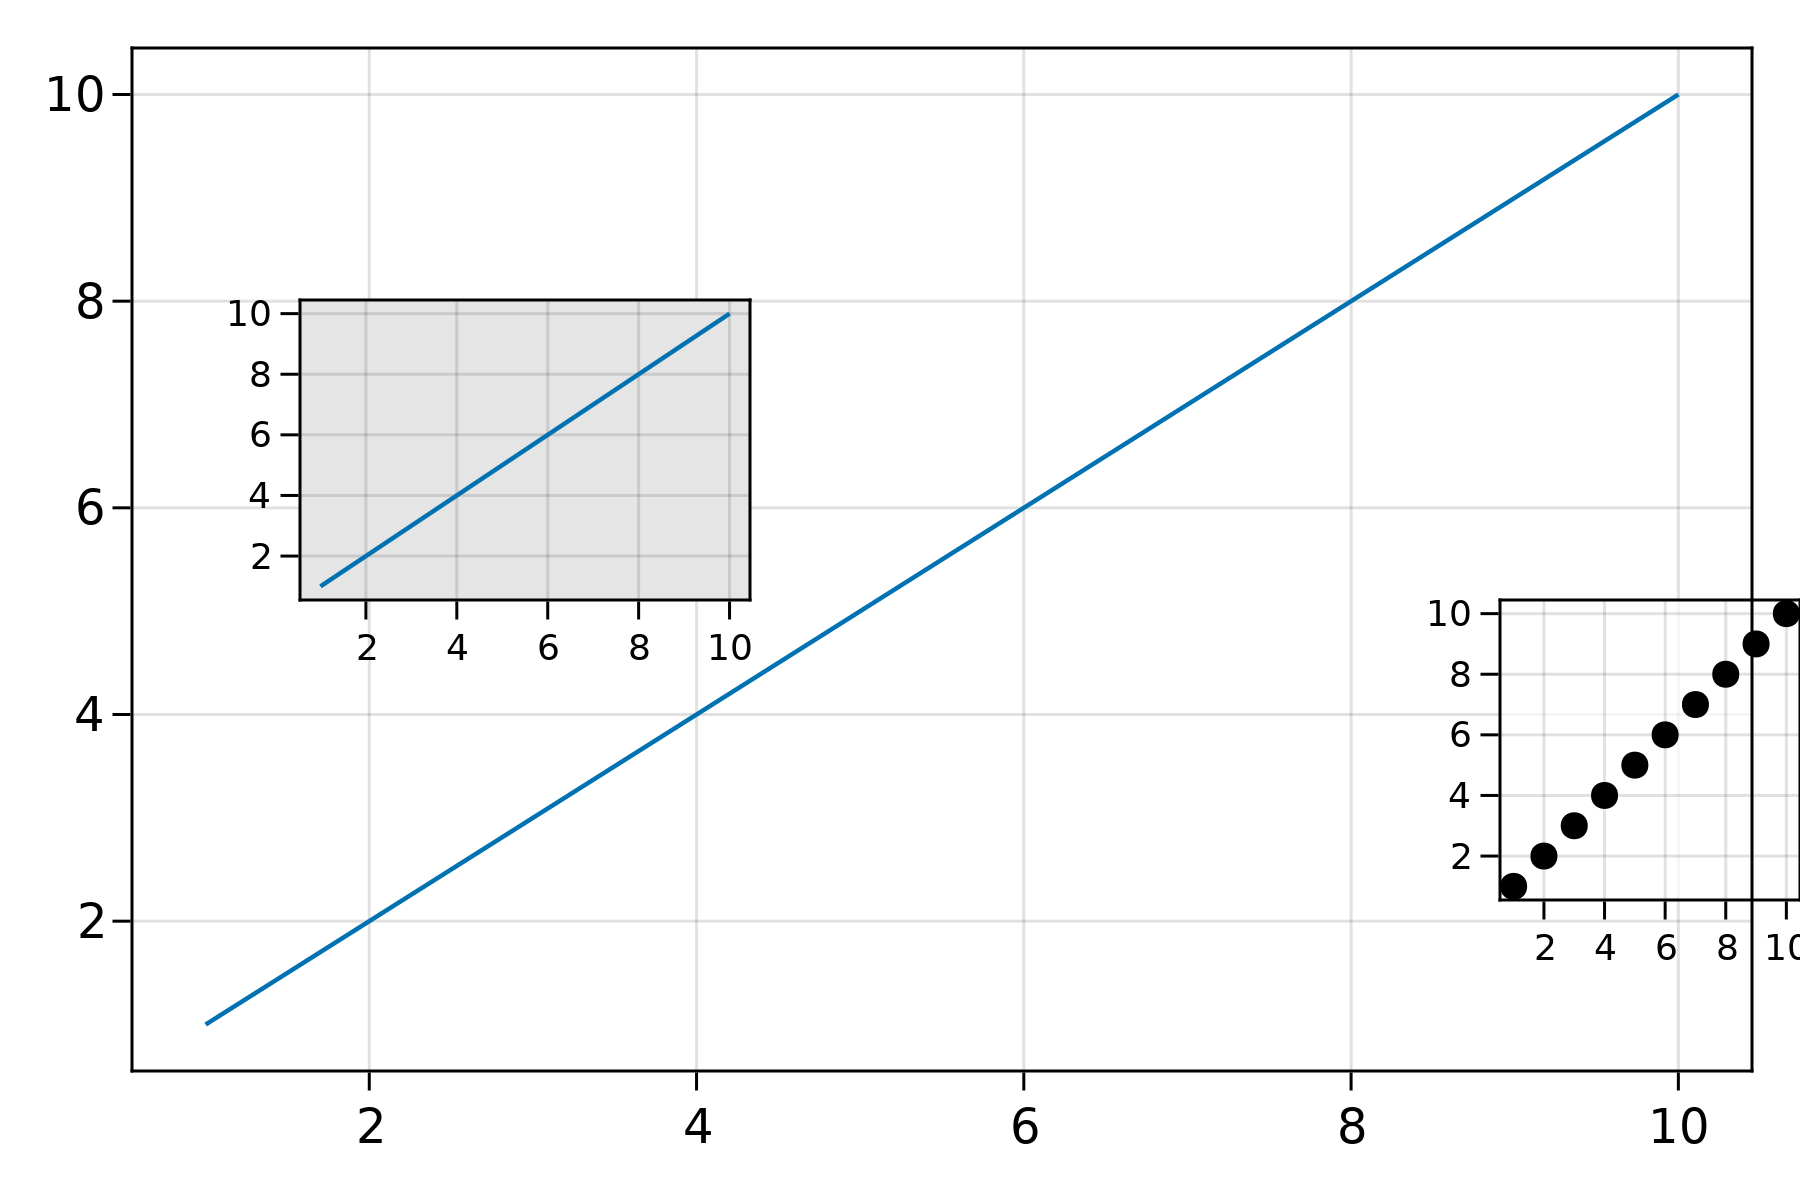
\includegraphics[width=0.6\textwidth,height=\textheight]{_build/im/JDS_figure_box_inset_.png}
\caption{Figure box inset.}\label{fig:figure_box_inset}
}
\end{figure}

where the \passthrough{\lstinline!Box!} dimensions are bound by the
\passthrough{\lstinline!Figure!}'s \passthrough{\lstinline!resolution!}.
Note, that an inset can be also outside the
\passthrough{\lstinline!Axis!}. The other approach, is by defining a new
\passthrough{\lstinline!Axis!} into a position
\passthrough{\lstinline!fig[i, j]!} specifying his
\passthrough{\lstinline!width!}, \passthrough{\lstinline!height!},
\passthrough{\lstinline!halign!} and \passthrough{\lstinline!valign!}.
We do that in the following function:

\begin{lstlisting}[language=Julia]
function add_axis_inset(pos=fig[1, 1]; halign, valign, width=Relative(0.5),
        height=Relative(0.35), alignmode=Mixed(left = 5, right=5), bgcolor=:lightgray)

    inset_box = Axis(pos; width, height, halign, valign, alignmode,
        xticklabelsize=12, yticklabelsize=12, backgroundcolor=bgcolor)
    # bring content upfront
    translate!(inset_box.scene, 0, 0, 10)
    return inset_box
end
\end{lstlisting}

See that in the following example the \passthrough{\lstinline!Axis!}
with gray background will be rescaled if the total figure size changes.
The \emph{insets} are bound by the \passthrough{\lstinline!Axis!}
positioning.

\begin{lstlisting}[language=Julia]
function figure_axis_inset()
    fig = Figure(resolution=(600, 400))
    ax = Axis(fig[1, 1], backgroundcolor=:white)
    inset_ax1 = add_axis_inset(fig[1, 1]; halign=:left, valign=:center,
        width=Relative(0.3), height=Relative(0.35),
        alignmode=Mixed(left=5, right=5, bottom=15),
        bgcolor = :grey90)
    inset_ax2 = add_axis_inset(fig[1, 1]; halign=:right, valign=:center,
        width=Relative(0.25), height=Relative(0.3), bgcolor=(:white, 0.65))
    lines!(ax, 1:10)
    lines!(inset_ax1, 1:10)
    scatter!(inset_ax2, 1:10, color=:black)
    fig
end
figure_axis_inset()
\end{lstlisting}

\begin{figure}
\hypertarget{fig:figure_axis_inset}{%
\centering
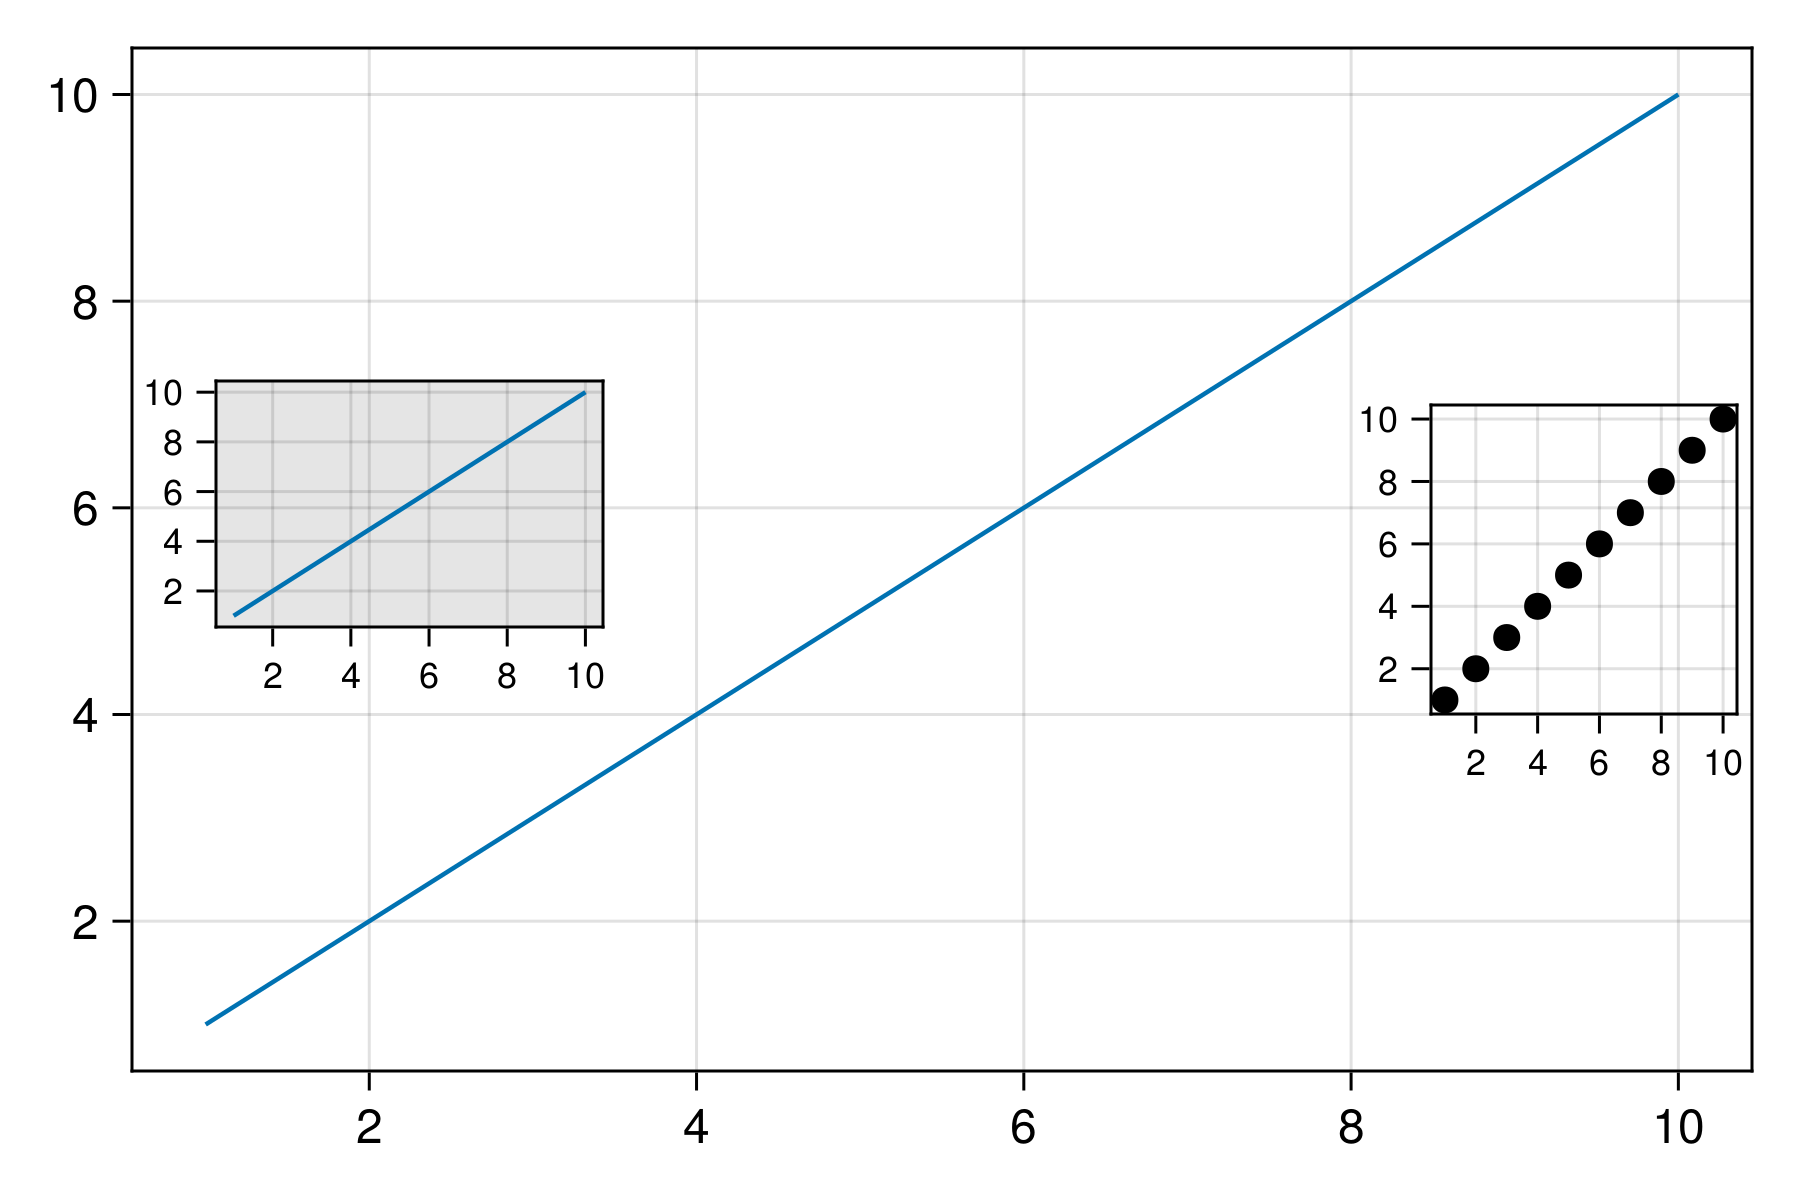
\includegraphics[width=0.6\textwidth,height=\textheight]{_build/im/JDS_figure_axis_inset_.png}
\caption{Figure axis inset.}\label{fig:figure_axis_inset}
}
\end{figure}

And this should cover most used cases for layouting with Makie. Now,
let's do some nice 3D examples with
\passthrough{\lstinline!GLMakie.jl!}.

\hypertarget{sec:glmakie}{%
\section{GLMakie.jl}\label{sec:glmakie}}

\passthrough{\lstinline!CairoMakie.jl!} supplies all our needs for
static 2D images. But sometimes we want interactivity, especially when
we are dealing with 3D images. Visualizing data in 3D is also a common
practice to gain insight from your data. This is where
\passthrough{\lstinline!GLMakie.jl!} might be helpful, since it uses
\href{http://www.opengl.org/}{OpenGL} as a backend that adds
interactivity and responsiveness to plots. Like before, a simple plot
includes, of course, lines and points. So, we will start with those and
since we already know how layouts work, we will put that into practice.

\hypertarget{scatters-and-lines}{%
\subsection{Scatters and Lines}\label{scatters-and-lines}}

For scatter plots we have two options, the first one is
\passthrough{\lstinline!scatter(x, y, z)!} and the second one is
\passthrough{\lstinline!meshscatter(x, y, z)!}. In the first one markers
don't scale in the axis directions, but in the latter they do because
they are actual geometries in 3D space. See the next example:

\begin{lstlisting}
using GLMakie
GLMakie.activate!()
\end{lstlisting}

\begin{lstlisting}[language=Julia]
function scatters_in_3D()
    seed!(123)
    xyz = randn(10, 3)
    x, y, z = xyz[:, 1], xyz[:, 2], xyz[:, 3]
    fig = Figure(resolution=(1200, 400))
    ax1 = Axis3(fig[1, 1]; aspect=(1, 1, 1), perspectiveness=0.5)
    ax2 = Axis3(fig[1, 2]; aspect=(1, 1, 1), perspectiveness=0.5)
    ax3 = Axis3(fig[1, 3]; aspect=:data, perspectiveness=0.5)
    scatter!(ax1, x, y, z; markersize=15)
    meshscatter!(ax2, x, y, z; markersize=0.25)
    hm = meshscatter!(ax3, x, y, z; markersize=0.25,
        marker=Rect3f(Vec3f(0), Vec3f(1)), color=1:size(xyz,2),
        colormap=:plasma, transparency=false)
    Colorbar(fig[1, 4], hm, label="values", height=Relative(0.5))
    fig
end
scatters_in_3D()
\end{lstlisting}

\begin{figure}
\hypertarget{fig:scatters_in_3D}{%
\centering
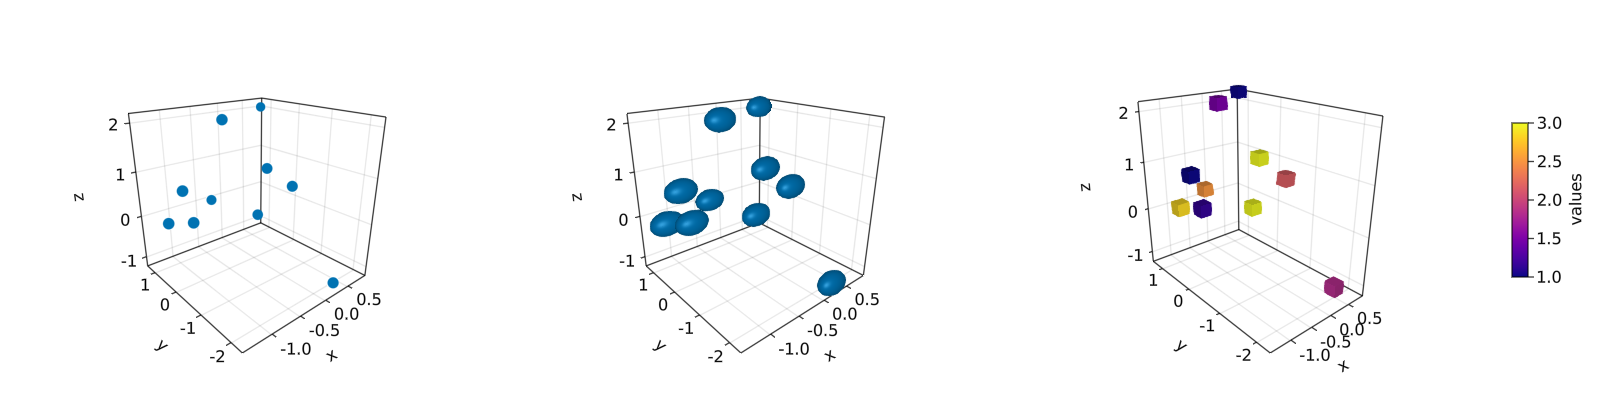
\includegraphics{_build/im/JDS_scatters_in_3D_.png}
\caption{Scatters in 3D.}\label{fig:scatters_in_3D}
}
\end{figure}

Note also, that a different geometry can be passed as markers, i.e., a
square/rectangle, and we can assign a \passthrough{\lstinline!colormap!}
for them as well. In the middle panel one could get perfect spheres by
doing \passthrough{\lstinline!aspect = :data!} as in the right panel.

And doing \passthrough{\lstinline!lines!} or
\passthrough{\lstinline!scatterlines!} is also straightforward:

\begin{lstlisting}[language=Julia]
function lines_in_3D()
    seed!(123)
    xyz = randn(10, 3)
    x, y, z = xyz[:, 1], xyz[:, 2], xyz[:, 3]
    fig = Figure(resolution=(1200, 500))
    ax1 = Axis3(fig[1, 1]; aspect=(1, 1, 1), perspectiveness=0.5)
    ax2 = Axis3(fig[1, 2]; aspect=(1, 1, 1), perspectiveness=0.5)
    ax3 = Axis3(fig[1, 3]; aspect=:data, perspectiveness=0.5)
    lines!(ax1, x, y, z; color=1:size(xyz)[2], linewidth=3)
    scatterlines!(ax2, x, y, z; markersize=15)
    hm = meshscatter!(ax3, x, y, z; markersize=0.2, color=1:size(xyz,2))
    lines!(ax3, x, y, z; color=1:size(xyz,2))
    Colorbar(fig[2, 1], hm; label="values", height=15, vertical=false,
        flipaxis=false, ticksize=15, tickalign=1, width=Relative(3.55 / 4))
    fig
end
lines_in_3D()
\end{lstlisting}

\begin{figure}
\hypertarget{fig:lines_in_3D}{%
\centering
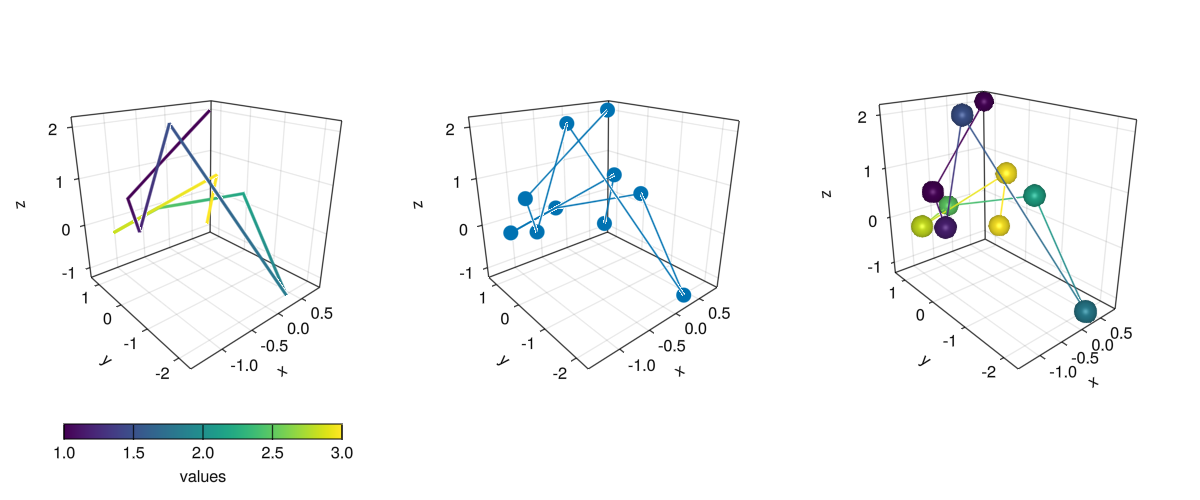
\includegraphics{_build/im/JDS_lines_in_3D_.png}
\caption{Lines in 3D.}\label{fig:lines_in_3D}
}
\end{figure}

Plotting a \passthrough{\lstinline!surface!} is also easy to do as well
as a \passthrough{\lstinline!wireframe!} and
\passthrough{\lstinline!contour!} lines in 3D.

\hypertarget{surfaces-wireframe-contour-contourf-and-contour3d}{%
\subsection{Surfaces, wireframe, contour, contourf and
contour3d}\label{surfaces-wireframe-contour-contourf-and-contour3d}}

To show these cases we'll use the following
\passthrough{\lstinline!peaks!} function:

\begin{lstlisting}[language=Julia]
function peaks(; n=49)
    x = LinRange(-3, 3, n)
    y = LinRange(-3, 3, n)
    a = 3 * (1 .- x') .^ 2 .* exp.(-(x' .^ 2) .- (y .+ 1) .^ 2)
    b = 10 * (x' / 5 .- x' .^ 3 .- y .^ 5) .* exp.(-x' .^ 2 .- y .^ 2)
    c = 1 / 3 * exp.(-(x' .+ 1) .^ 2 .- y .^ 2)
    return (x, y, a .- b .- c)
end
\end{lstlisting}

The output for the different plotting functions is

\begin{lstlisting}[language=Julia]
function plot_peaks_function()
    x, y, z = peaks()
    x2, y2, z2 = peaks(; n=15)
    fig = Figure(resolution=(1200, 400))
    axs = [Axis3(fig[1, i]; aspect=(1, 1, 1)) for i = 1:3]
    hm = surface!(axs[1], x, y, z)
    wireframe!(axs[2], x2, y2, z2)
    contour3d!(axs[3], x, y, z; levels=20)
    Colorbar(fig[1, 4], hm, height=Relative(0.5))
    fig
end
plot_peaks_function()
\end{lstlisting}

\begin{figure}
\hypertarget{fig:plot_peaks_function}{%
\centering
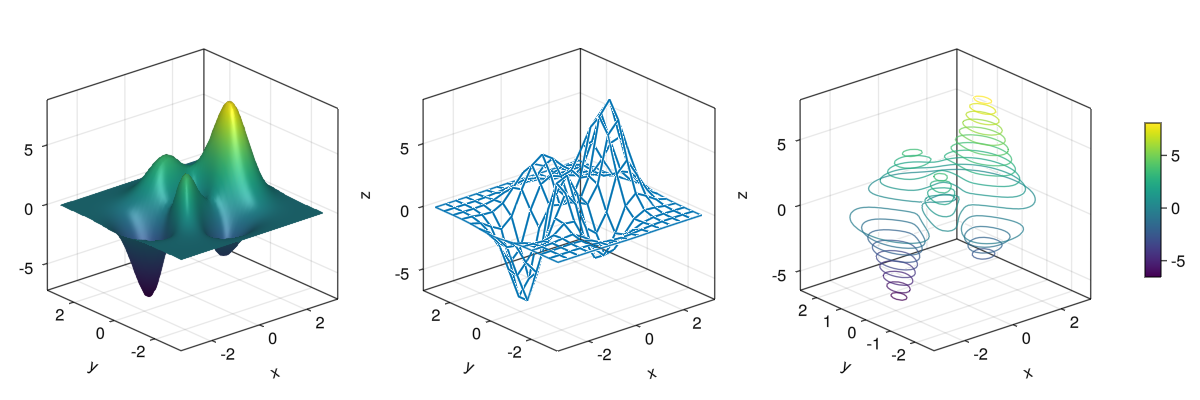
\includegraphics{_build/im/JDS_plot_peaks_function_.png}
\caption{Plot peaks function.}\label{fig:plot_peaks_function}
}
\end{figure}

But, it can also be plotted with a
\passthrough{\lstinline!heatmap(x, y, z)!},
\passthrough{\lstinline!contour(x, y, z)!} or
\passthrough{\lstinline!contourf(x, y, z)!}:

\begin{lstlisting}[language=Julia]
function heatmap_contour_and_contourf()
    x, y, z = peaks()
    fig = Figure(resolution=(1200, 400))
    axs = [Axis(fig[1, i]; aspect=DataAspect()) for i = 1:3]
    hm = heatmap!(axs[1], x, y, z)
    contour!(axs[2], x, y, z; levels=20)
    contourf!(axs[3], x, y, z)
    Colorbar(fig[1, 4], hm, height=Relative(0.5))
    fig
end
heatmap_contour_and_contourf()
\end{lstlisting}

\begin{figure}
\hypertarget{fig:heatmap_contour_and_contourf}{%
\centering
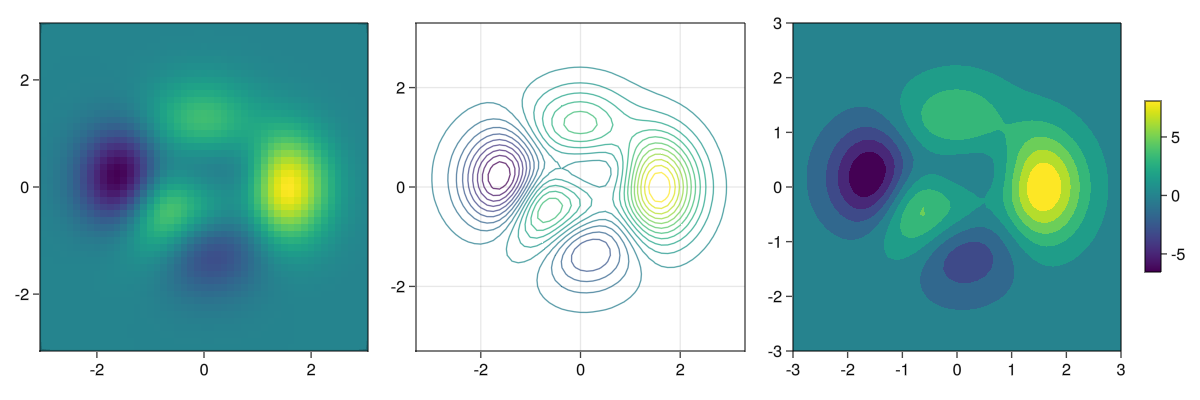
\includegraphics{_build/im/JDS_heatmap_contour_and_contourf_.png}
\caption{Heatmap contour and
contourf.}\label{fig:heatmap_contour_and_contourf}
}
\end{figure}

Additionally, by changing \passthrough{\lstinline!Axis!} to an
\passthrough{\lstinline!Axis3!}, these plots will be automatically be in
the x-y plane:

\begin{lstlisting}[language=Julia]
function heatmap_contour_and_contourf_in_a_3d_plane()
    x, y, z = peaks()
    fig = Figure(resolution=(1200, 400))
    axs = [Axis3(fig[1, i]) for i = 1:3]
    hm = heatmap!(axs[1], x, y, z)
    contour!(axs[2], x, y, z; levels=20)
    contourf!(axs[3], x, y, z)
    Colorbar(fig[1, 4], hm, height=Relative(0.5))
    fig
end
heatmap_contour_and_contourf_in_a_3d_plane()
\end{lstlisting}

\begin{figure}
\hypertarget{fig:heatmap_contour_and_contourf_in_a_3d_plane}{%
\centering
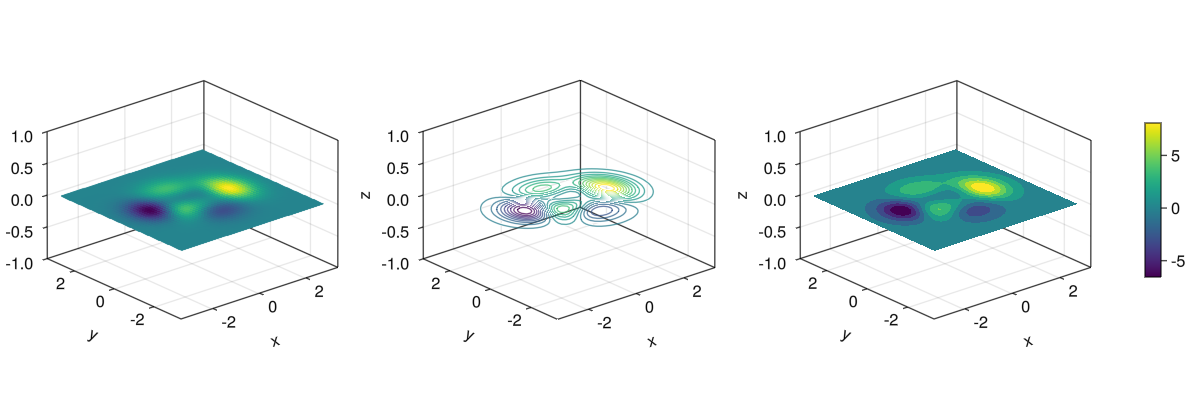
\includegraphics{_build/im/JDS_heatmap_contour_and_contourf_in_a_3d_plane_.png}
\caption{Heatmap contour and contourf in a 3d
plane.}\label{fig:heatmap_contour_and_contourf_in_a_3d_plane}
}
\end{figure}

Something else that is easy to do is to mix all these plotting functions
into just one plot, namely:

\begin{lstlisting}
using TestImages
\end{lstlisting}

\begin{lstlisting}[language=Julia]
function mixing_surface_contour3d_contour_and_contourf()
    img = testimage("coffee.png")
    x, y, z = peaks()
    cmap = :Spectral_11
    fig = Figure(resolution=(1200, 800), fontsize=26)
    ax1 = Axis3(fig[1, 1]; aspect=(1, 1, 1), elevation=pi / 6, xzpanelcolor=(:black, 0.75),
        perspectiveness=0.5, yzpanelcolor=:black, zgridcolor=:grey70,
        ygridcolor=:grey70, xgridcolor=:grey70)
    ax2 = Axis3(fig[1, 3]; aspect=(1, 1, 1), elevation=pi / 6, perspectiveness=0.5)
    hm = surface!(ax1, x, y, z; colormap=(cmap, 0.95), shading=true)
    contour3d!(ax1, x, y, z .+ 0.02; colormap=cmap, levels=20, linewidth=2)
    xmin, ymin, zmin = minimum(ax1.finallimits[])
    xmax, ymax, zmax = maximum(ax1.finallimits[])
    contour!(ax1, x, y, z; colormap=cmap, levels=20, transformation=(:xy, zmax))
    contourf!(ax1, x, y, z; colormap=cmap, transformation=(:xy, zmin))
    Colorbar(fig[1, 2], hm, width=15, ticksize=15, tickalign=1, height=Relative(0.35))
    # transformations into planes
    heatmap!(ax2, x, y, z; colormap=:viridis, transformation=(:yz, 3.5))
    contourf!(ax2, x, y, z; colormap=:CMRmap, transformation=(:xy, -3.5))
    contourf!(ax2, x, y, z; colormap=:bone_1, transformation=(:xz, 3.5))
    image!(ax2, -3 .. 3, -3 .. 2, rotr90(img); transformation=(:xy, 3.8))
    xlims!(ax2, -3.8, 3.8)
    ylims!(ax2, -3.8, 3.8)
    zlims!(ax2, -3.8, 3.8)
    fig
end
mixing_surface_contour3d_contour_and_contourf()
\end{lstlisting}

\begin{figure}
\hypertarget{fig:mixing_surface_contour3d_contour_and_contourf}{%
\centering
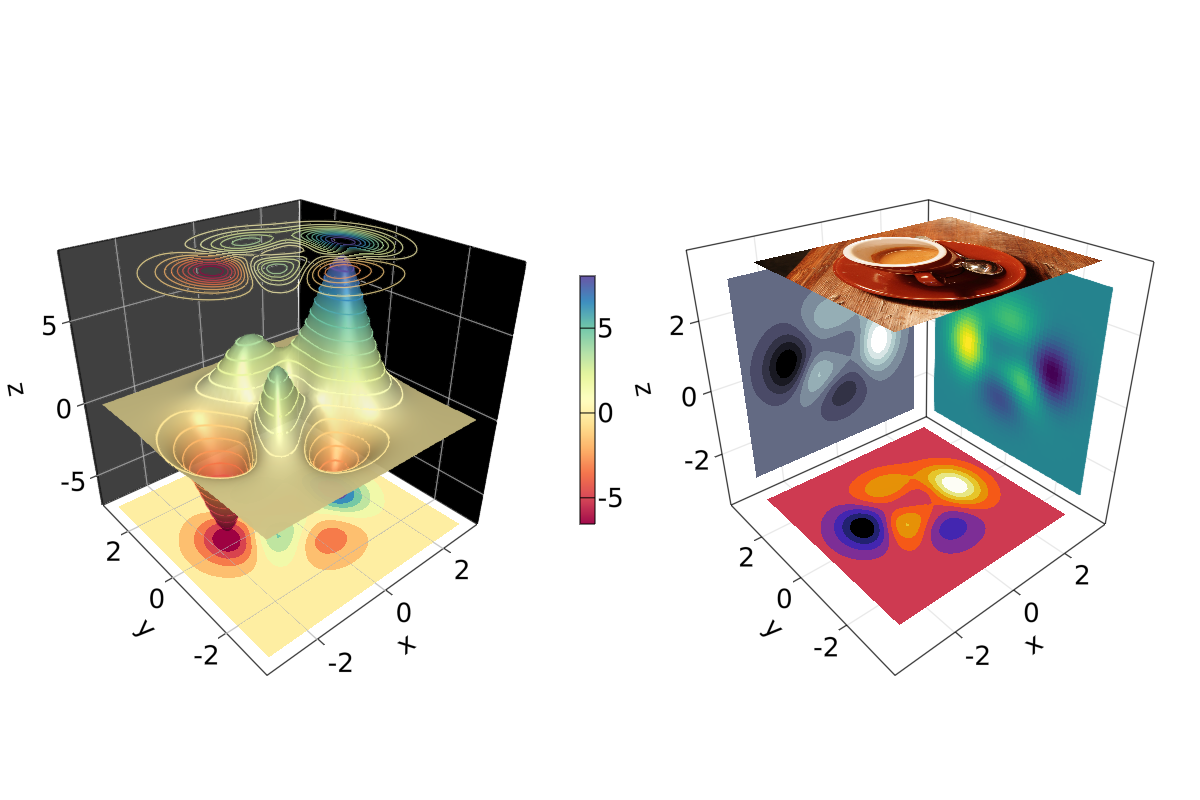
\includegraphics[width=0.6\textwidth,height=\textheight]{_build/im/JDS_mixing_surface_contour3d_contour_and_contourf_.png}
\caption{Mixing surface, contour3d, contour and
contourf.}\label{fig:mixing_surface_contour3d_contour_and_contourf}
}
\end{figure}

Not bad, right? From there is clear that any
\passthrough{\lstinline!heatmap!}'s,
\passthrough{\lstinline!contour!}'s,
\passthrough{\lstinline!contourf!}'s or \passthrough{\lstinline!image!}
can be plotted into any plane.

\hypertarget{arrows-and-streamplots}{%
\subsection{Arrows and Streamplots}\label{arrows-and-streamplots}}

\passthrough{\lstinline!arrows!} and
\passthrough{\lstinline!streamplot!} are plots that might be useful when
we want to know the directions that a given variable will follow. See a
demonstration below\footnote{we are using the
  \passthrough{\lstinline!LinearAlgebra!} module from Julia's standard
  library.}:

\begin{lstlisting}
using LinearAlgebra
\end{lstlisting}

\begin{lstlisting}[language=Julia]
function arrows_and_streamplot_in_3d()
    ps = [Point3f(x, y, z) for x = -3:1:3 for y = -3:1:3 for z = -3:1:3]
    ns = map(p -> 0.1 * rand() * Vec3f(p[2], p[3], p[1]), ps)
    lengths = norm.(ns)
    flowField(x, y, z) = Point(-y + x * (-1 + x^2 + y^2)^2, x + y * (-1 + x^2 + y^2)^2,
        z + x * (y - z^2))
    fig = Figure(resolution=(1200, 800), fontsize=26)
    axs = [Axis3(fig[1, i]; aspect=(1, 1, 1), perspectiveness=0.5) for i = 1:2]
    arrows!(axs[1], ps, ns, color=lengths, arrowsize=Vec3f(0.2, 0.2, 0.3),
        linewidth=0.1)
    streamplot!(axs[2], flowField, -4 .. 4, -4 .. 4, -4 .. 4, colormap=:plasma,
        gridsize=(7, 7), arrow_size=0.25, linewidth=1)
    fig
end
arrows_and_streamplot_in_3d()
\end{lstlisting}

\begin{figure}
\hypertarget{fig:arrows_and_streamplot_in_3d}{%
\centering
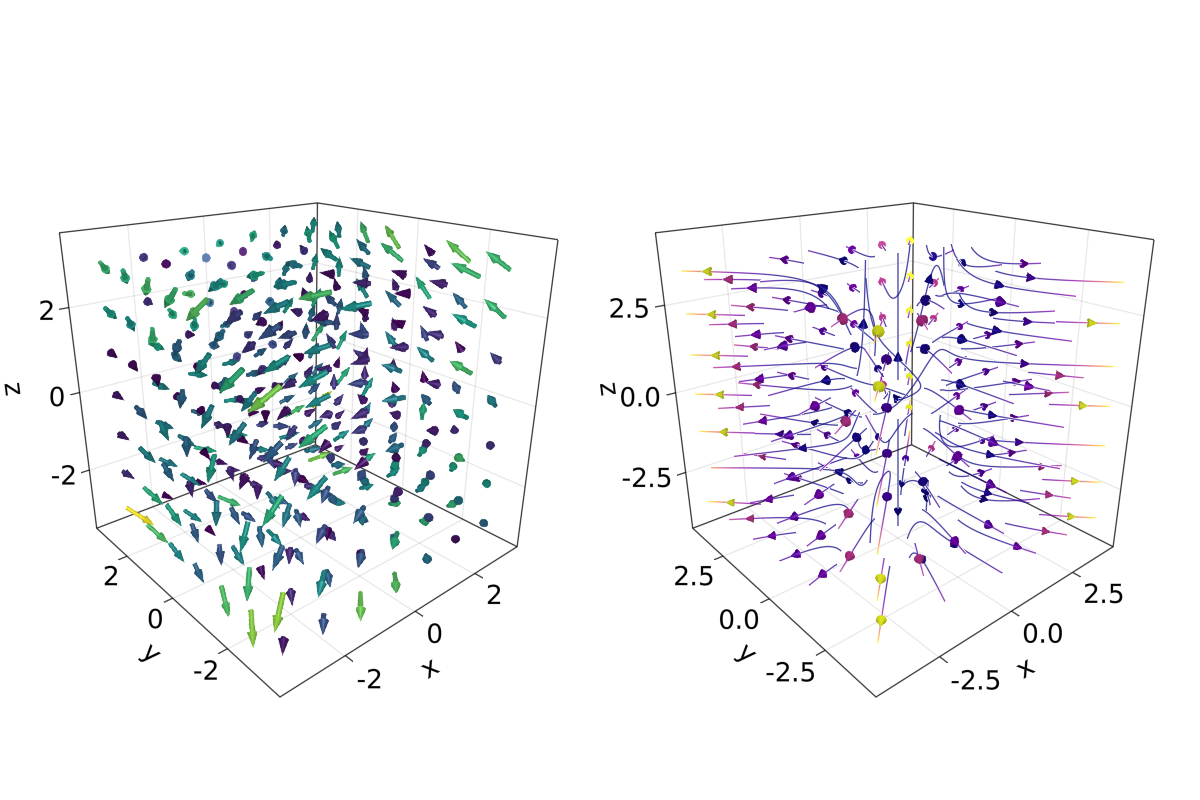
\includegraphics[width=0.6\textwidth,height=\textheight]{_build/im/JDS_arrows_and_streamplot_in_3d_.png}
\caption{Arrows and streamplot in
3d.}\label{fig:arrows_and_streamplot_in_3d}
}
\end{figure}

Other interesting examples are a \passthrough{\lstinline!mesh(obj)!}, a
\passthrough{\lstinline!volume(x, y, z, vals)!}, and a
\passthrough{\lstinline!contour(x, y, z, vals)!}.

\hypertarget{meshes-and-volumes}{%
\subsection{Meshes and Volumes}\label{meshes-and-volumes}}

Drawing meshes comes in handy when you want to plot geometries, like a
\passthrough{\lstinline!Sphere!} or a Rectangle,
i.e.~\passthrough{\lstinline!FRect3D!}. Another approach to visualize
points in 3D space is by calling the functions
\passthrough{\lstinline!volume!} and \passthrough{\lstinline!contour!},
which implements
\href{https://en.wikipedia.org/wiki/Ray_tracing_(graphics)}{ray tracing}
to simulate a wide variety of optical effects. See the next examples:

\begin{lstlisting}
using GeometryBasics
\end{lstlisting}

\begin{lstlisting}[language=Julia]
function mesh_volume_contour()
    # mesh objects
    rectMesh = Rect3f(Vec3f(-0.5), Vec3f(1))
    recmesh = GeometryBasics.mesh(rectMesh)
    sphere = Sphere(Point3f(0), 1)
    # https://juliageometry.github.io/GeometryBasics.jl/stable/primitives/
    spheremesh = GeometryBasics.mesh(Tesselation(sphere, 64))
    # uses 64 for tesselation, a smoother sphere
    colors = [rand() for v in recmesh.position]
    # cloud points for volume
    x = y = z = 1:10
    vals = randn(10, 10, 10)
    fig = Figure(resolution=(1200, 400))
    axs = [Axis3(fig[1, i]; aspect=(1, 1, 1), perspectiveness=0.5) for i = 1:3]
    mesh!(axs[1], recmesh; color=colors, colormap=:rainbow, shading=false)
    mesh!(axs[1], spheremesh; color=(:white, 0.25), transparency=true)
    volume!(axs[2], x, y, z, vals; colormap=Reverse(:plasma))
    contour!(axs[3], x, y, z, vals; colormap=Reverse(:plasma))
    fig
end
mesh_volume_contour()
\end{lstlisting}

\begin{figure}
\hypertarget{fig:mesh_volume_contour}{%
\centering
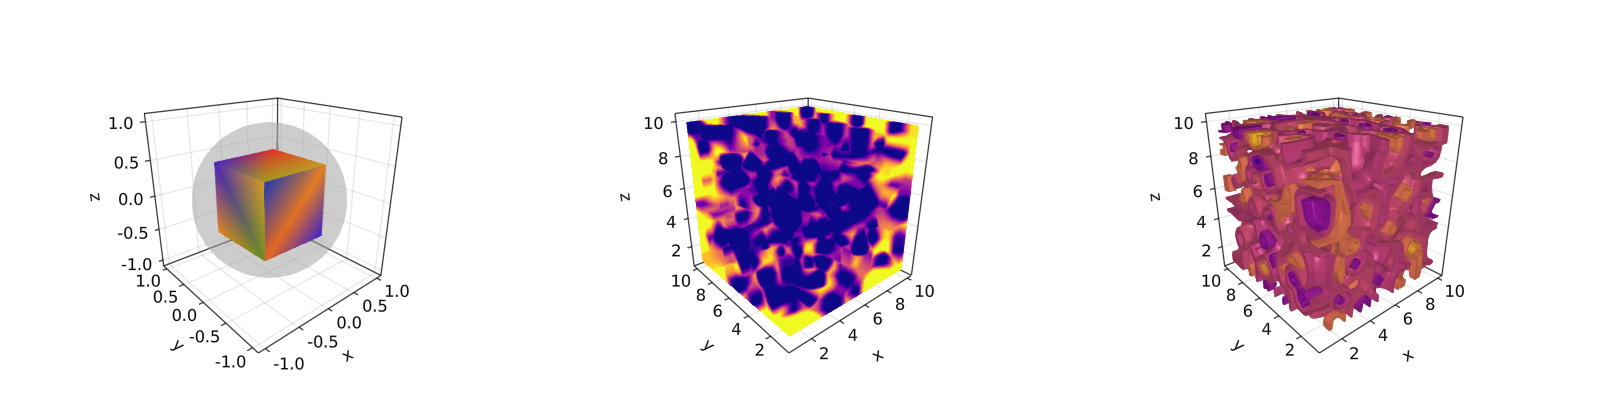
\includegraphics{_build/im/JDS_mesh_volume_contour_.png}
\caption{Mesh volume contour.}\label{fig:mesh_volume_contour}
}
\end{figure}

Note that here we are plotting two meshes in the same axis, one
transparent sphere and a cube. So far, we have covered most of the 3D
use-cases.

Taking as reference the previous example one can do the following custom
plot with spheres and rectangles:

\begin{lstlisting}
using GeometryBasics, Colors
\end{lstlisting}

For the spheres let's do a rectangular grid. Also, we will use a
different color for each one of them. Additionally, we can mix spheres
and a rectangular plane. Next, we define all the necessary data.

\begin{lstlisting}[language=Julia]
seed!(123)
spheresGrid = [Point3f(i,j,k) for i in 1:2:12 for j in 1:2:10 for k in 1:2:10]
colorSphere = [RGBA(i * 0.1, j * 0.1, k * 0.1, 0.75) for i in 1:2:12 for j in 1:2:10 for k in 1:2:10]
spheresPlane = [Point3f(i,j,k) for i in 1:2.5:20 for j in 1:2.5:10 for k in 1:2.5:4]
cmap = get(colorschemes[:plasma], LinRange(0, 1, 50))
colorsPlane = cmap[rand(1:50,50)]
rectMesh = Rect3f(Vec3f(-1, -1, 2.1), Vec3f(22, 11, 0.5))
recmesh = GeometryBasics.mesh(rectMesh)
colors = [RGBA(rand(4)...) for v in recmesh.position]
\end{lstlisting}

Then, the plot is simply done with:

\begin{lstlisting}[language=Julia]
function grid_spheres_and_rectangle_as_plate()
    fig = with_theme(theme_dark()) do
        fig = Figure(resolution=(1200, 800))
        ax1 = Axis3(fig[1, 1]; aspect=:data, perspectiveness=0.5, azimuth=0.72)
        ax2 = Axis3(fig[1, 2]; aspect=:data, perspectiveness=0.5)
        meshscatter!(ax1, spheresGrid; color = colorSphere, markersize = 1,
            shading=false)
        meshscatter!(ax2, spheresPlane; color=colorsPlane, markersize = 0.75,
            lightposition=Vec3f(10, 5, 2), ambient=Vec3f(0.95, 0.95, 0.95),
            backlight=1.0f0)
        mesh!(recmesh; color=colors, colormap=:rainbow, shading=false)
        limits!(ax1, 0, 10, 0, 10, 0, 10)
        fig
    end
    fig
end
grid_spheres_and_rectangle_as_plate()
\end{lstlisting}

\begin{figure}
\hypertarget{fig:grid_spheres_and_rectangle_as_plate}{%
\centering
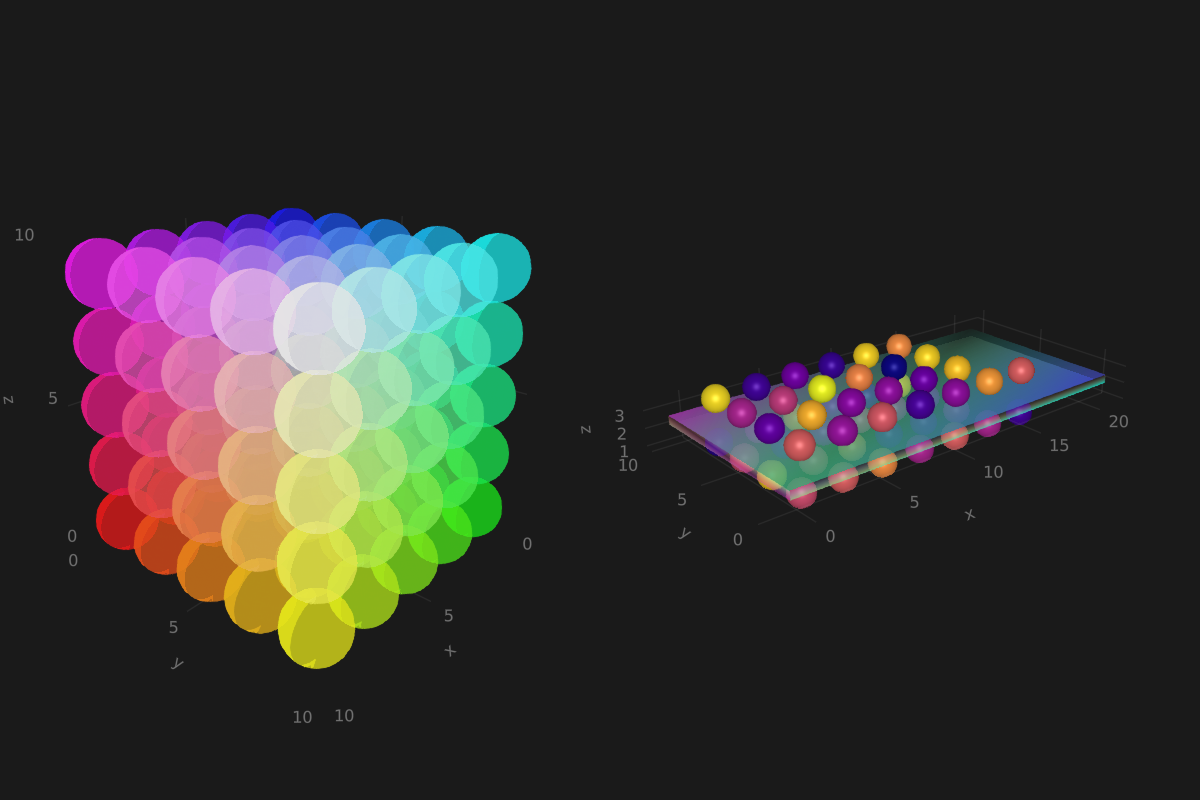
\includegraphics[width=0.6\textwidth,height=\textheight]{_build/im/JDS_grid_spheres_and_rectangle_as_plate_.png}
\caption{Grid spheres and rectangle as
plate.}\label{fig:grid_spheres_and_rectangle_as_plate}
}
\end{figure}

Here, the rectangle is semi-transparent due to the alpha channel added
to the RGB color. The rectangle function is quite versatile, for
instance 3D boxes are easy to implement which in turn could be used for
plotting a 3D histogram. See our next example, where we are using again
our \passthrough{\lstinline!peaks!} function and some additional
definitions:

\begin{lstlisting}[language=Julia]
x, y, z = peaks(; n=15)
δx = (x[2] - x[1]) / 2
δy = (y[2] - y[1]) / 2
cbarPal = :Spectral_11
ztmp = (z .- minimum(z)) ./ (maximum(z .- minimum(z)))
cmap = get(colorschemes[cbarPal], ztmp)
cmap2 = reshape(cmap, size(z))
ztmp2 = abs.(z) ./ maximum(abs.(z)) .+ 0.15
\end{lstlisting}

here \(\delta x, \delta y\) are used to specify our boxes size.
\passthrough{\lstinline!cmap2!} will be the color for each box and
\passthrough{\lstinline!ztmp2!} will be used as a transparency
parameter. See the output in the next figure.

\begin{lstlisting}[language=Julia]
function histogram_or_bars_in_3d()
    fig = Figure(resolution=(1200, 800), fontsize=26)
    ax1 = Axis3(fig[1, 1]; aspect=(1, 1, 1), elevation=π/6,
        perspectiveness=0.5)
    ax2 = Axis3(fig[1, 2]; aspect=(1, 1, 1), perspectiveness=0.5)
    rectMesh = Rect3f(Vec3f(-0.5, -0.5, 0), Vec3f(1, 1, 1))
    meshscatter!(ax1, x, y, 0*z, marker = rectMesh, color = z[:],
        markersize = Vec3f.(2δx, 2δy, z[:]), colormap = :Spectral_11,
        shading=false)
    limits!(ax1, -3.5, 3.5, -3.5, 3.5, -7.45, 7.45)
    meshscatter!(ax2, x, y, 0*z, marker = rectMesh, color = z[:],
        markersize = Vec3f.(2δx, 2δy, z[:]), colormap = (:Spectral_11, 0.25),
        shading=false, transparency=true)
    for (idx, i) in enumerate(x), (idy, j) in enumerate(y)
        rectMesh = Rect3f(Vec3f(i - δx, j - δy, 0), Vec3f(2δx, 2δy, z[idx, idy]))
        recmesh = GeometryBasics.mesh(rectMesh)
        lines!(ax2, recmesh; color=(cmap2[idx, idy], ztmp2[idx, idy]))
    end
    fig
end
histogram_or_bars_in_3d()
\end{lstlisting}

\begin{figure}
\hypertarget{fig:histogram_or_bars_in_3d}{%
\centering
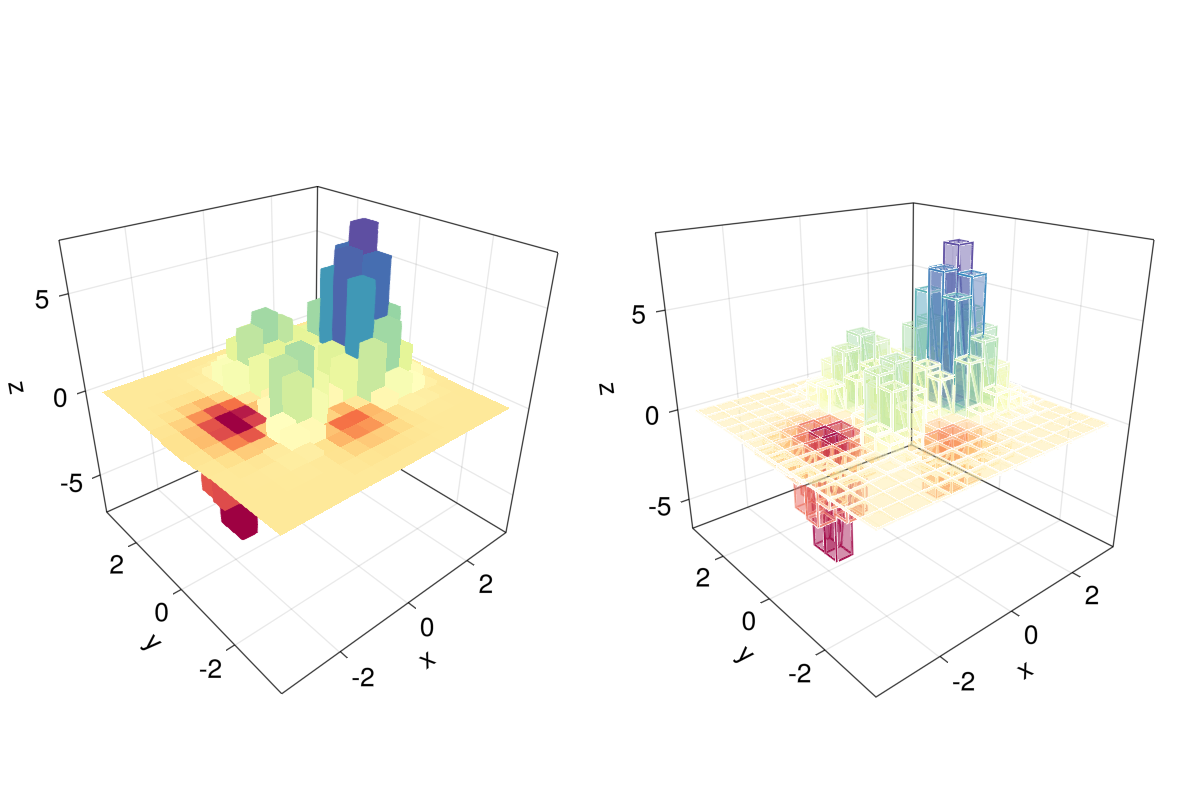
\includegraphics[width=0.6\textwidth,height=\textheight]{_build/im/JDS_histogram_or_bars_in_3d_.png}
\caption{Histogram or bars in 3d.}\label{fig:histogram_or_bars_in_3d}
}
\end{figure}

Note, that you can also call \passthrough{\lstinline!lines!} or
\passthrough{\lstinline!wireframe!} over a mesh object.

\hypertarget{filled-line-and-band}{%
\subsection{Filled Line and Band}\label{filled-line-and-band}}

For our last example we will show how to do a filled curve in 3D with
\passthrough{\lstinline!band!} and some
\passthrough{\lstinline!linesegments!}:

\begin{lstlisting}[language=Julia]
function filled_line_and_linesegments_in_3D()
    xs = LinRange(-3, 3, 10)
    lower = [Point3f(i, -i, 0) for i in LinRange(0, 3, 100)]
    upper = [Point3f(i, -i, sin(i) * exp(-(i + i))) for i in range(0, 3, length=100)]
    fig = Figure(resolution=(1200, 800))
    axs = [Axis3(fig[1, i]; elevation=pi/6, perspectiveness=0.5) for i = 1:2]
    band!(axs[1], lower, upper, color=repeat(norm.(upper), outer=2), colormap=:CMRmap)
    lines!(axs[1], upper, color=:black)
    linesegments!(axs[2], cos.(xs), xs, sin.(xs), linewidth=5, color=1:length(xs))
    fig
end
filled_line_and_linesegments_in_3D()
\end{lstlisting}

\begin{figure}
\hypertarget{fig:filled_line_and_linesegments_in_3D}{%
\centering
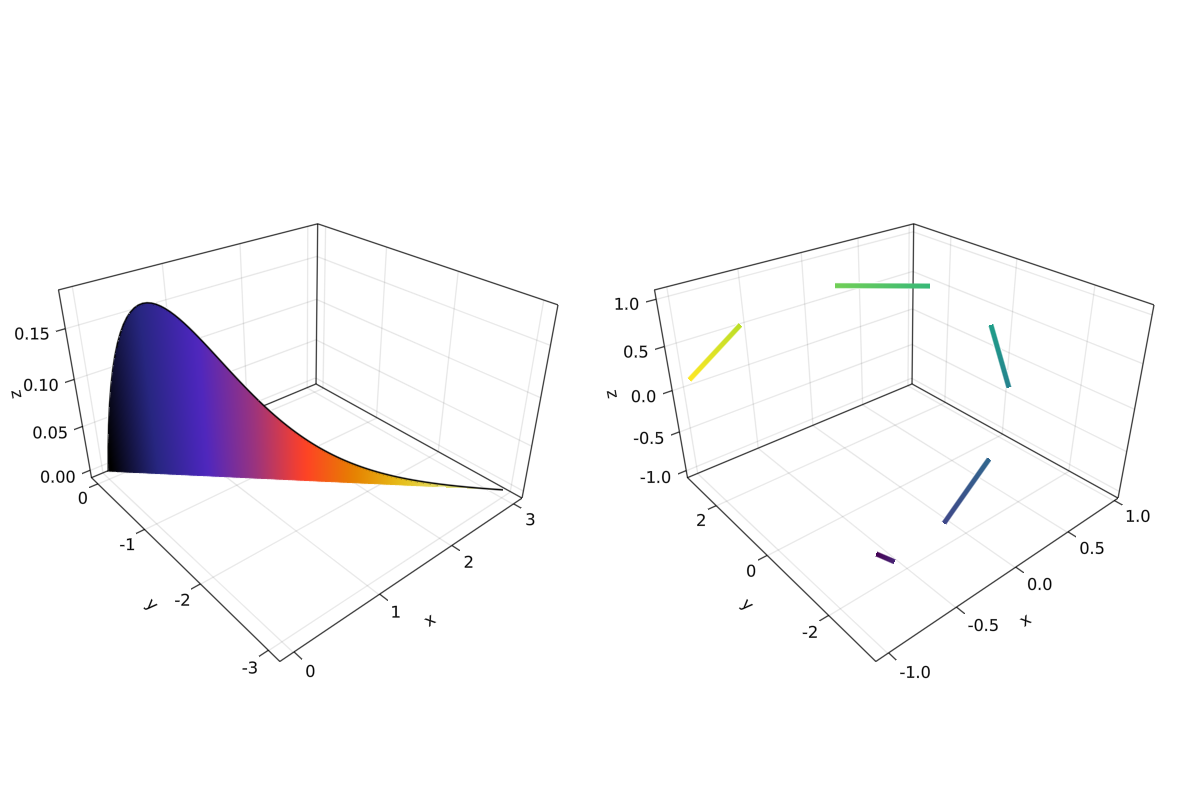
\includegraphics[width=0.6\textwidth,height=\textheight]{_build/im/JDS_filled_line_and_linesegments_in_3D_.png}
\caption{Filled line and linesegments in
3D.}\label{fig:filled_line_and_linesegments_in_3D}
}
\end{figure}

Finally, our journey doing 3D plots has come to an end. You can combine
everything we exposed here to create amazing 3D images!

\hypertarget{sec:recipe_df}{%
\section{A Makie recipe for a DataFrame}\label{sec:recipe_df}}

Unlike other libraries that already support a wide set of input formats
via recipes, i.e.~\passthrough{\lstinline!Plots.jl!}, in
\passthrough{\lstinline!Makie.jl!} most of the time we need to pass the
raw data to functions. However, we can also define our own
\passthrough{\lstinline!recipe!} in \passthrough{\lstinline!Makie.jl!}.
A \passthrough{\lstinline!recipe!} is your own custom plotting type
command. This extension is done just in
\passthrough{\lstinline!Makie.jl!}, which means that making a new set of
plotting rules for your own types is light, namely, you don't need the
complete plotting machinery available to define them. This is specially
useful if you want to include your own plotting commands in one of your
own packages. However, in order for them to work you will still need to
use one of the backends, i.e., GLMakie or CairoMakie.

As an example we will code a small \textbf{full recipe} for a
\passthrough{\lstinline!DataFrame!}. Please refer to the
\href{https://makie.juliaplots.org/stable/documentation/recipes/}{documentation}
for more details.

A Makie \passthrough{\lstinline!recipe!} consist of two parts, a plot
\passthrough{\lstinline!type!} name defined via
\passthrough{\lstinline!@recipe!} and a custom
\passthrough{\lstinline"plot!(::Makie.plot)"} which creates the actual
plot via plotting functions already defined.

\begin{lstlisting}[language=Julia]
@recipe(DfPlot, df) do scene
    Attributes(
        x = :A,
        y = :B,
        c = :C,
        color = :red,
        colormap = :plasma,
        markersize = 20,
        marker = :rect,
        colorrange = (0,1),
        label = "",
    )
end
\end{lstlisting}

Note that the macro \passthrough{\lstinline!@recipe!} will automatically
create two new functions for us, \passthrough{\lstinline!dfplot!} and
\passthrough{\lstinline"dfplot!"}, all lowercase from our type
\passthrough{\lstinline!DfPlot!}. The first one will create a complete
new figure whereas the second one will plot into the current axis or an
axis of your choosing. This allows us to plot
\passthrough{\lstinline!DataFrame!}s which contains columns named,
\passthrough{\lstinline!x!}, \passthrough{\lstinline!y!},
\passthrough{\lstinline!z!}. Now, let's take care of our plot
definition. We will do a simple scatter plot:

\begin{lstlisting}
import Makie
\end{lstlisting}

\begin{lstlisting}[language=Julia]
function Makie.plot!(p::DfPlot{<:Tuple{<:DataFrame}})
    df = p[:df][]
    x = getproperty(df, p[:x][])
    y = getproperty(df, p[:y][])
    c = getproperty(df, p[:c][])
    scatter!(p, x, y; color = c, markersize = p[:markersize][],
        colormap = p[:colormap][], marker = p[:marker][],
        colorrange = (minimum(x), maximum(c)), label = p[:label][])
    return p
end
\end{lstlisting}

Note the extras \passthrough{\lstinline![]!} at the end of each
variable. Those are due to the fact that \emph{recipes} in Makie are
dynamic, meaning that our plots will update if our variables change. See
\href{https://makie.juliaplots.org/stable/documentation/nodes/}{observables}
to know more. Now, we apply our new plotting function to the following
\passthrough{\lstinline!DataFrame!}:

\begin{lstlisting}[language=Julia]
df_recipe = DataFrame(A=randn(10), B=randn(10), C=rand(10))
\end{lstlisting}

\begin{lstlisting}[language=Julia]
fig, ax, obj = dfplot(df_recipe; label = "test")
axislegend()
Colorbar(fig[1,2], obj)
fig
\end{lstlisting}

\begin{figure}
\hypertarget{fig:dfRecipe}{%
\centering
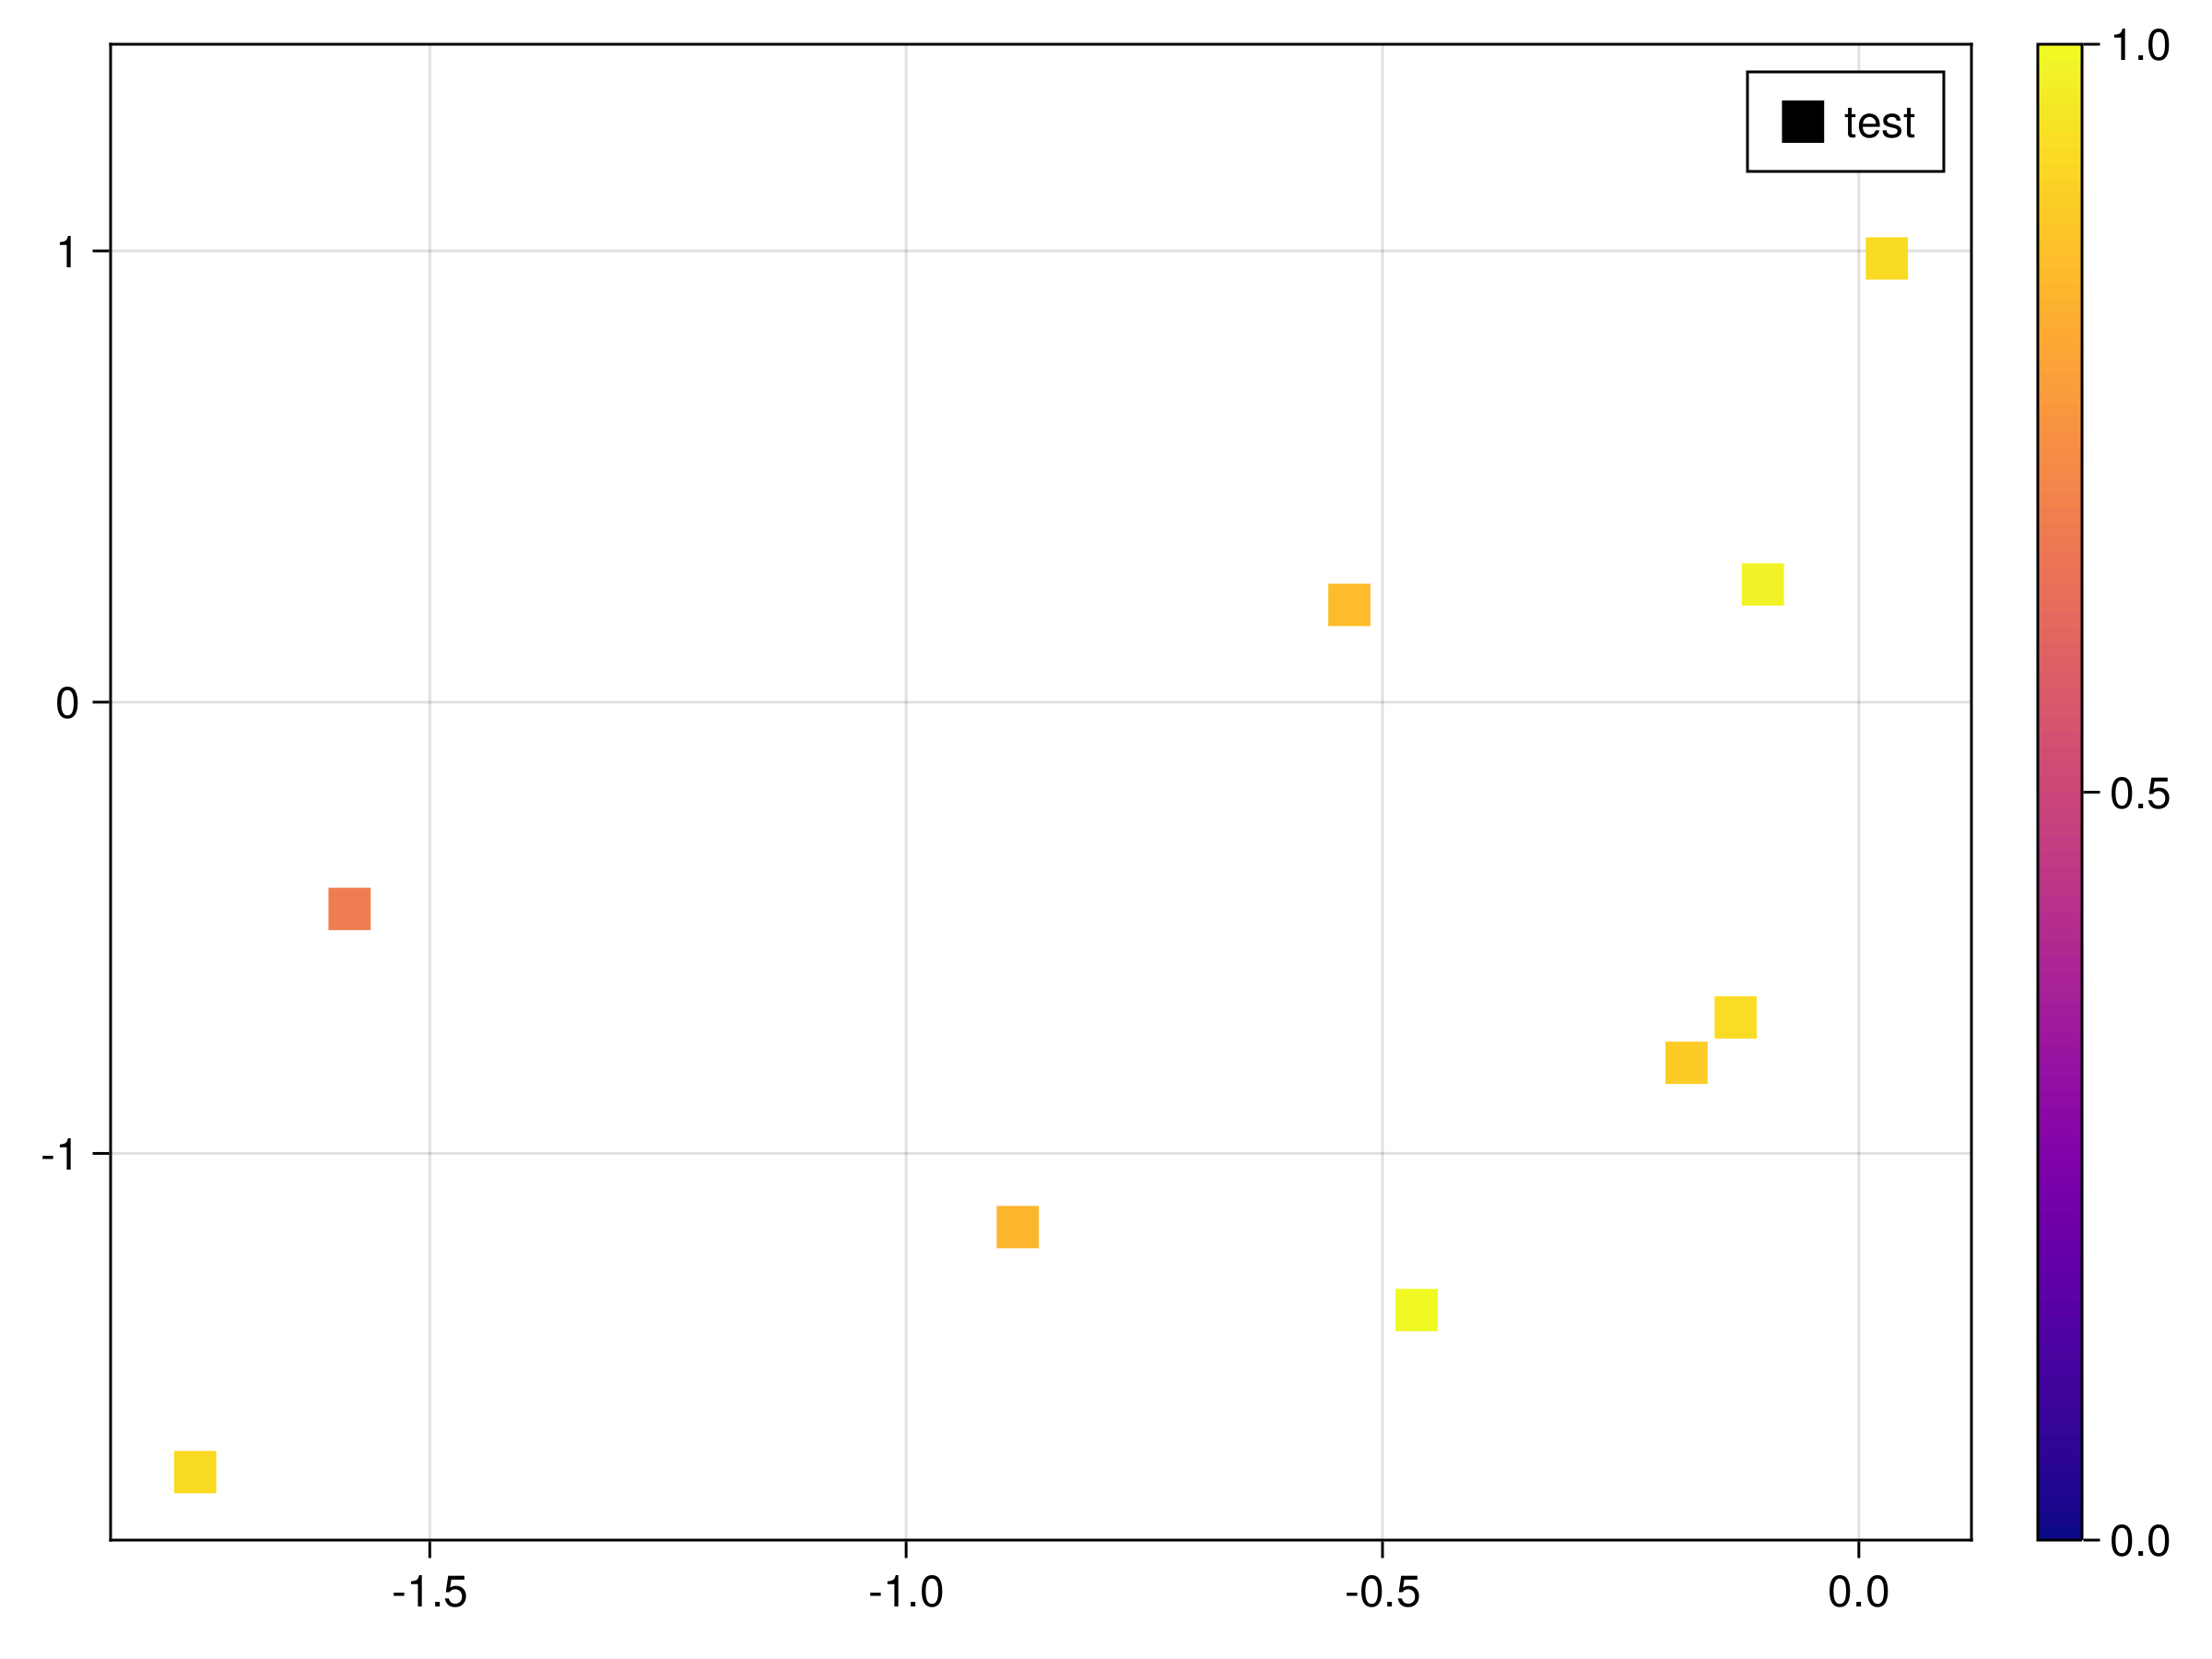
\includegraphics[width=0.6\textwidth,height=\textheight]{_build/im/dfRecipe.png}
\caption{DataFrames recipe.}\label{fig:dfRecipe}
}
\end{figure}

The named attributes in the recipe allows us to pass custom names to our
new plotting function. Namely:

\begin{lstlisting}[language=Julia]
df_names = DataFrame(a1=rand(100), a2=rand(100), a3=rand(100))
\end{lstlisting}

and:

\begin{lstlisting}[language=Julia]
dfplot(df_names; x = :a1, y = :a2, c = :a3, marker = 'o',
    axis = (; aspect=1, xlabel = "a1", ylabel = "a2"),
    figure = (; backgroundcolor = :grey90))
\end{lstlisting}

\begin{figure}
\hypertarget{fig:dfRecipeArgs}{%
\centering
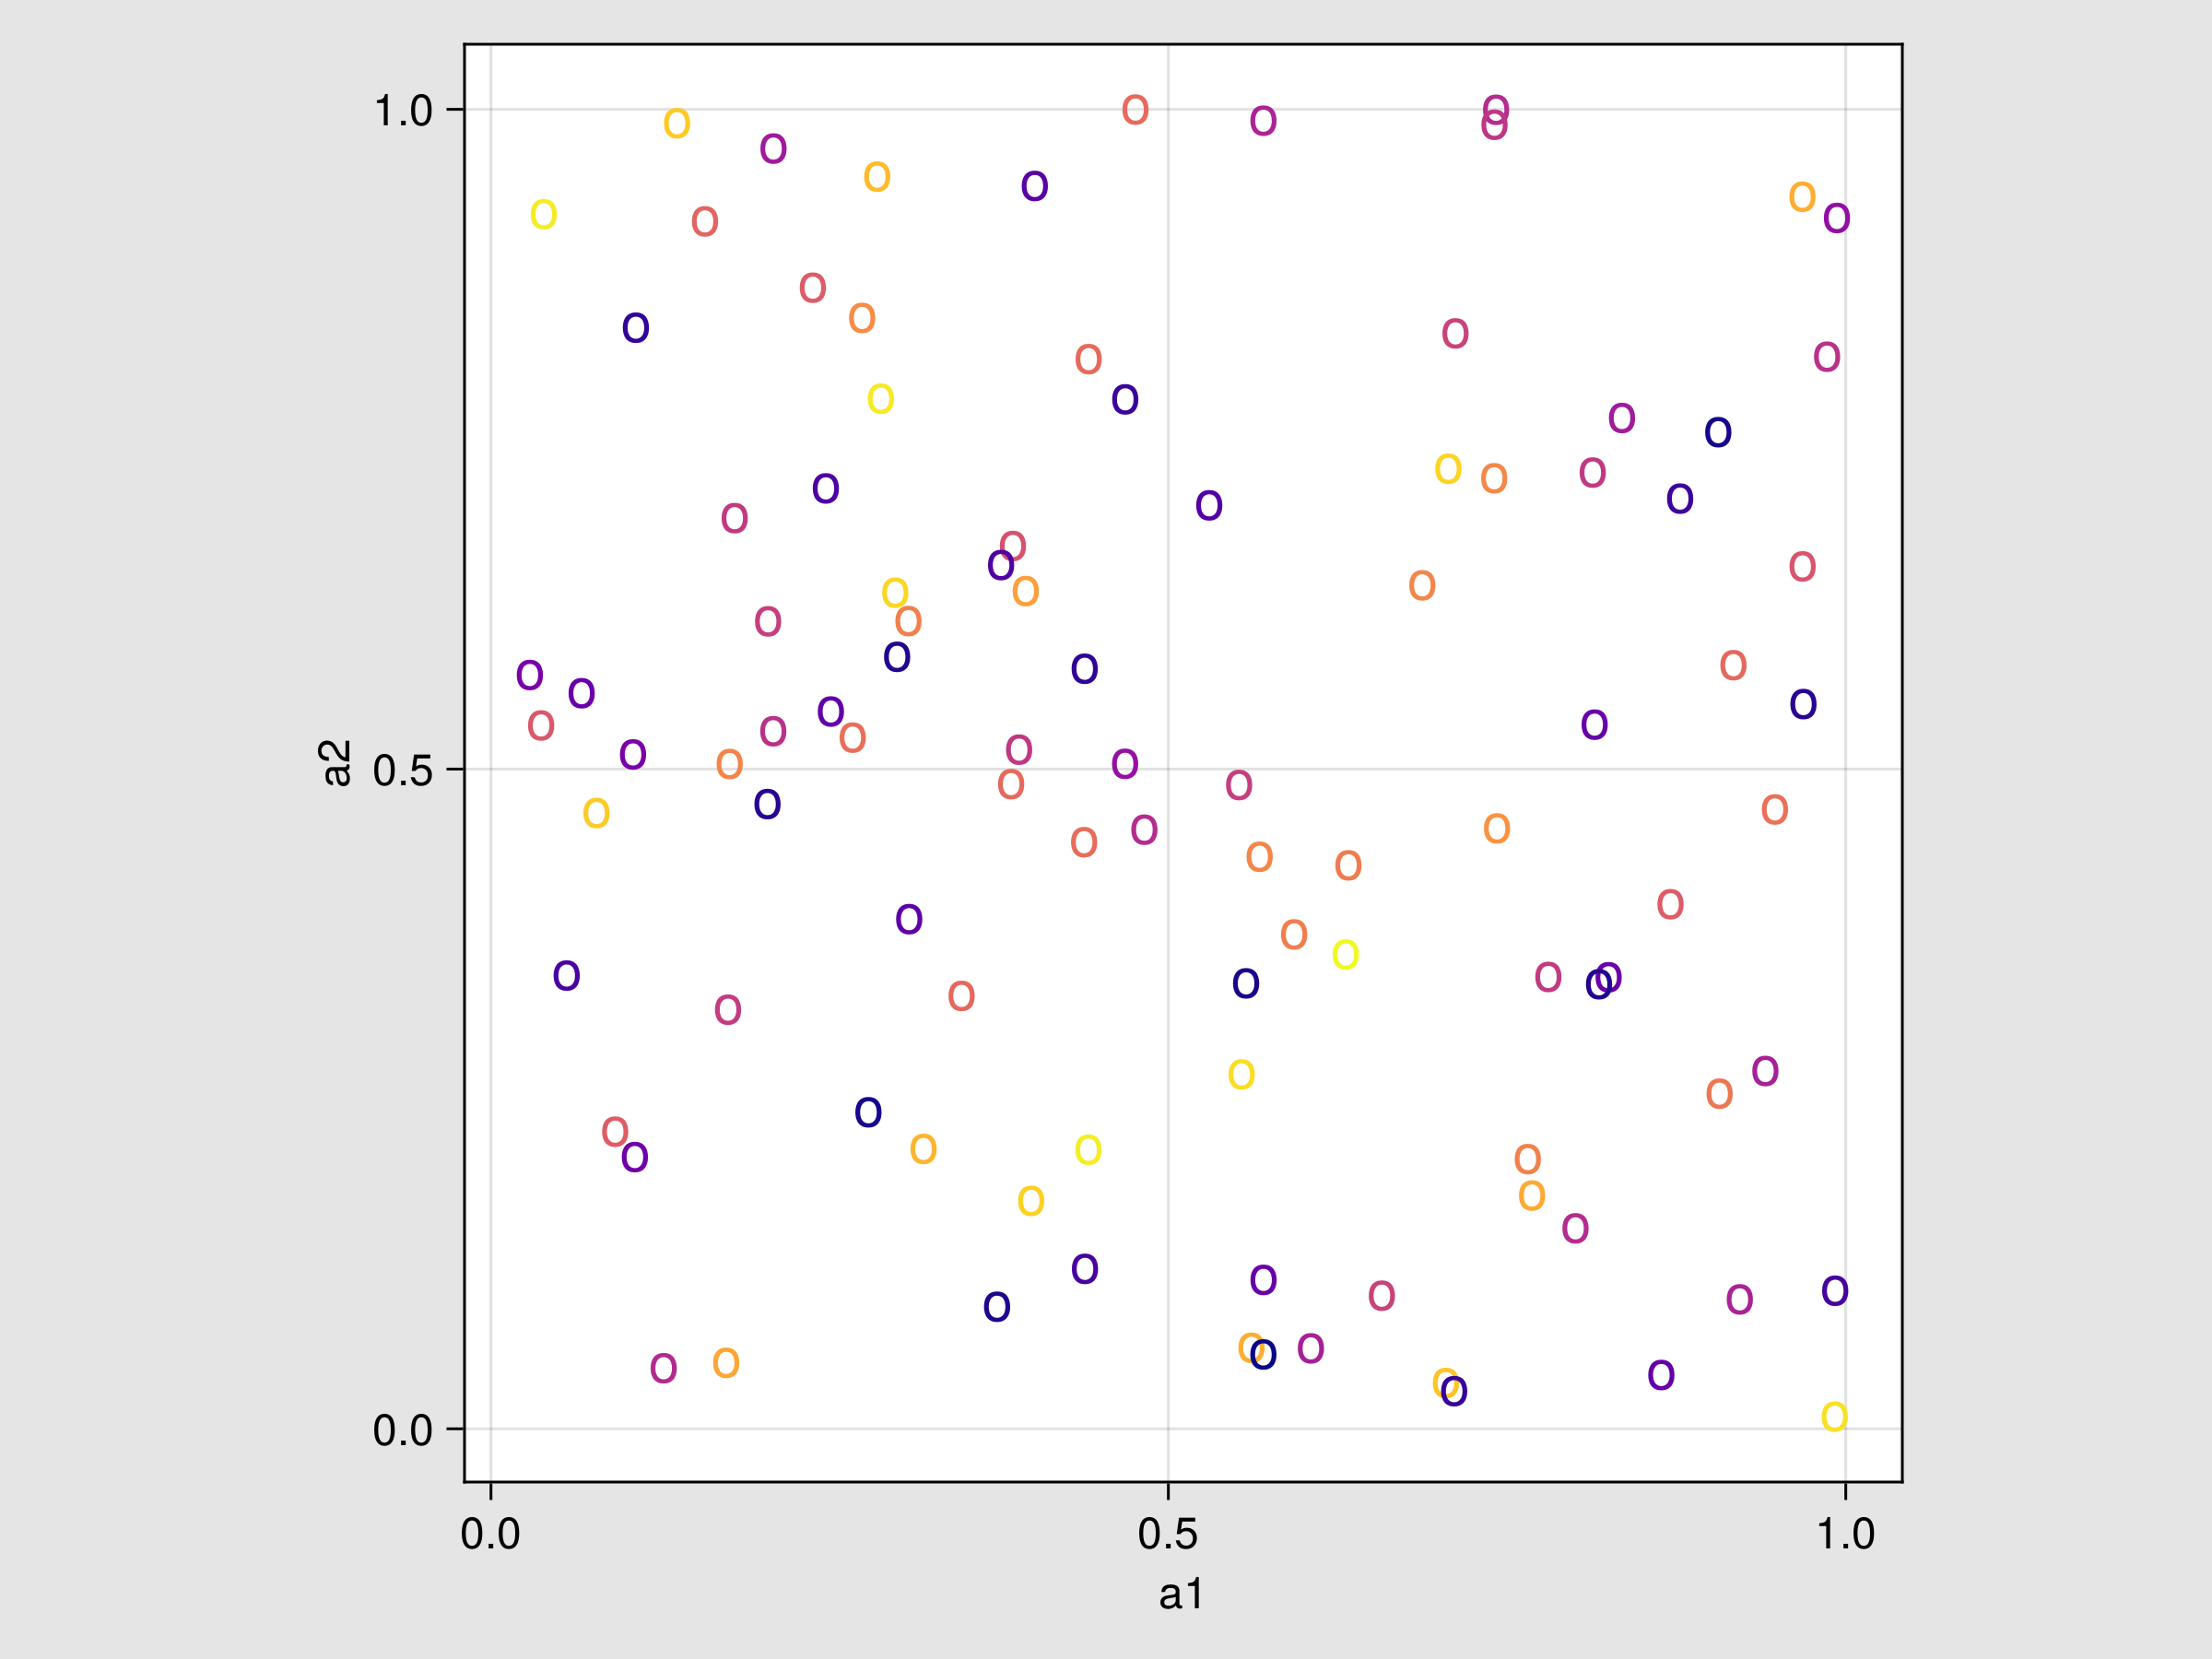
\includegraphics[width=0.6\textwidth,height=\textheight]{_build/im/dfRecipeArgs.png}
\caption{DataFrames recipe with arguments.}\label{fig:dfRecipeArgs}
}
\end{figure}

Note, that now we are calling by name each column as well as the marker
type, allowing us to use this definition for different DataFrames.
Additionally, all our previous options, i.e.,
\passthrough{\lstinline!axis!} or \passthrough{\lstinline!figure!} also
work!

\hypertarget{sec:appendix}{%
\chapter{Appendix}\label{sec:appendix}}

\hypertarget{sec:appendix_pkg}{%
\section{Packages Versions}\label{sec:appendix_pkg}}

This book is built with Julia 1.7.3 and the following packages:

\begin{lstlisting}[language=Julia]
Books 1.2.8
CSV 0.10.4
CairoMakie 0.8.3
CategoricalArrays 0.10.6
ColorSchemes 3.18.0
Colors 0.12.8
DataFrames 1.3.4
Distributions 0.25.62
FileIO 1.14.0
GLMakie 0.6.3
GeometryBasics 0.4.2
ImageMagick 1.2.2
LaTeXStrings 1.3.0
Makie 0.17.3
QuartzImageIO 0.7.4
Reexport 1.2.2
StatsBase 0.33.16
TestImages 1.7.0
XLSX 0.7.10
\end{lstlisting}

Build: 2022-06-08 21:45 UTC

\hypertarget{sec:notation}{%
\section{Notation}\label{sec:notation}}

In this book, we try to keep notation as consistent as possible. This
makes reading and writing code easier. We can define the notation into
three parts.

\hypertarget{julia-style-guide}{%
\subsection{Julia Style Guide}\label{julia-style-guide}}

Firstly, we attempt to stick to the conventions from the
\href{https://docs.julialang.org/en/v1/manual/style-guide/}{Julia Style
Guide}. Most importantly, we write functions not scripts (see also
Section~\ref{sec:engineering}). Furthermore, we use naming conventions
consistent with Julia \passthrough{\lstinline!base/!}, meaning:

\begin{itemize}
\tightlist
\item
  Use camelcase for modules:
  \passthrough{\lstinline!module JuliaDataScience!},
  \passthrough{\lstinline!struct MyPoint!}. (Note that camelcase is so
  called because the capitalization of words, as in ``iPad'' or
  ``CamelCase,'' makes the word look like a camel.)
\item
  Write function names in lowercase letters and separate the words by
  underscores. It is also allowed to omit the separator when naming
  functions. For example, these function names are all in line with the
  conventions: \passthrough{\lstinline!my\_function!},
  \passthrough{\lstinline!myfunction!} and
  \passthrough{\lstinline!string2int!}.
\end{itemize}

Also, we avoid brackets in conditionals, that is, we write
\passthrough{\lstinline!if a == b!} instead of
\passthrough{\lstinline!if (a == b)!} and use 4 spaces per indentation
level.

\hypertarget{bluestyle}{%
\subsection{BlueStyle}\label{bluestyle}}

The \href{https://github.com/invenia/BlueStyle}{Blue Style Guide} adds
multiple conventions on top of the default Julia Style Guide. Some of
these rules might sound pedantic, but we found that they make the code
more readable.

From the style guide, we attempt to adhere specifically to:

\begin{itemize}
\item
  At most 92 characters per line in code (in Markdown files, longer
  lines are allowed).
\item
  When loading code via \passthrough{\lstinline!using!}, load at most
  one module per line.
\item
  No trailing whitespace. Trailing whitespace makes inspecting changes
  in code more difficult since they do not change the behavior of the
  code but do show up as changes.
\item
  Avoid extraneous spaces inside brackets. So, write
  \passthrough{\lstinline!string(1, 2)!} instead of
  \passthrough{\lstinline!string( 1 , 2 )!}.
\item
  Global variables should be avoided.
\item
  Try to limit function names to one or two words.
\item
  Use the semicolon to clarify whether an argument is a keyword argument
  or not. For example, \passthrough{\lstinline!func(x; y=3)!} instead of
  \passthrough{\lstinline!func(x, y=3)!}.
\item
  Avoid using multiple spaces to align things. So, write

\begin{lstlisting}
a = 1
lorem = 2
\end{lstlisting}

  instead of

\begin{lstlisting}
a     = 1
lorem = 2
\end{lstlisting}
\item
  Whenever appropriate, surround binary operators with a space, for
  example, \passthrough{\lstinline!1 == 2!} or
  \passthrough{\lstinline!y = x + 1!}.
\item
  Indent triple-quotes and triple-backticks:

\begin{lstlisting}
s = """
    my long text:
    [...]
    the end.
    """
\end{lstlisting}
\item
  Do not omit zeros in floats (even though Julia allows it). Hence,
  write \passthrough{\lstinline!1.0!} instead of
  \passthrough{\lstinline!1.!} and write \passthrough{\lstinline!0.1!}
  instead of \passthrough{\lstinline!.1!}.
\item
  Use \passthrough{\lstinline!in!} in for loops and not = or ∈ (even
  though Julia allows it).
\end{itemize}

\hypertarget{our-additions}{%
\subsection{Our additions}\label{our-additions}}

\begin{itemize}
\tightlist
\item
  In text, we reference the function call
  \passthrough{\lstinline!M.foo(3, 4)!} as
  \passthrough{\lstinline!M.foo!} and not
  \passthrough{\lstinline!M.foo(...)!} or
  \passthrough{\lstinline!M.foo()!}.
\item
  When talking about packages, like the DataFrames package, we
  explicitly write \passthrough{\lstinline!DataFrames.jl!} each time.
  This makes it easier to recognize that we are talking about a package.
\item
  For filenames, we stick to ``file.txt'' and not
  \passthrough{\lstinline!file.txt!} or file.txt, because it is
  consistent with the code.
\item
  For column names in tables, like the column
  \passthrough{\lstinline!x!}, we stick to column
  \passthrough{\lstinline!:x!}, because it is consistent with the code.
\item
  Do not use Unicode symbols in inline code. This is simply a bug in the
  PDF generation that we have to workaround for now.
\item
  The line before each code block ends with a colon (:) to indicate that
  the line belongs to the code block.
\end{itemize}

\hypertarget{loading-of-symbols}{%
\subsubsection{Loading of symbols}\label{loading-of-symbols}}

Prefer to load symbols explicitly, that is, prefer
\passthrough{\lstinline!using A: foo!} over
\passthrough{\lstinline!using A!} when not using the REPL (see also,
\protect\hyperlink{ref-jump2021using}{\emph{JuMP Style Guide}, 2021}).
In this context, a symbol means an identifier to an object. For example,
even if it doesn't look like it normally, internally
\passthrough{\lstinline!DataFrame!}, \passthrough{\lstinline!π!} and
\passthrough{\lstinline!CSV!} are all symbols. We notice this when we
use an introspective method from Julia such as
\passthrough{\lstinline!isdefined!}:

\begin{lstlisting}[language=Julia]
isdefined(Main, :π)
\end{lstlisting}

\begin{lstlisting}[language=Output]
true
\end{lstlisting}

Next to being explicit when using \passthrough{\lstinline!using!}, also
prefer \passthrough{\lstinline!using A: foo!} over
\passthrough{\lstinline!import A: foo!} because the latter makes it easy
to accidentally extend \passthrough{\lstinline!foo!}. Note that this
isn't just advice for Julia: implicit loading of symbols via
\passthrough{\lstinline!from <module> import *!} is also discouraged in
Python (\protect\hyperlink{ref-pep8}{van Rossum et al., 2001}).

The reason why being explicit is important is related to semantic
versioning. With semantic versioning (\url{http://semver.org}), the
version number is related to whether a package is so-called
\emph{breaking} or not. For example, a non-breaking update for package
\passthrough{\lstinline!A!} is when the package goes from version
\passthrough{\lstinline!0.2.2!} to \passthrough{\lstinline!0.2.3!}. With
such a non-breaking version update, you don't need to worry that your
package will break, that is, throw an error or change behavior. If
package \passthrough{\lstinline!A!} goes from
\passthrough{\lstinline!0.2!} to \passthrough{\lstinline!1.0!}, then
that's a breaking update and you can expect that you need some changes
in your package to make \passthrough{\lstinline!A!} work again.
\textbf{However}, exporting extra symbols is considered a non-breaking
change. So, with implicit loading of symbols, \textbf{non-breaking
changes can break your package}. That's why it's good practice to
explicitly load symbols.

\hypertarget{references}{%
\chapter*{References}\label{references}}
\addcontentsline{toc}{chapter}{References}

\hypertarget{refs}{}
\begin{CSLReferences}{1}{0}
\leavevmode\hypertarget{ref-bezanson2017julia}{}%
Bezanson, J., Edelman, A., Karpinski, S., \& Shah, V. B. (2017). Julia:
{A} fresh approach to numerical computing. \emph{SIAM Review},
\emph{59}(1), 65--98.

\leavevmode\hypertarget{ref-chen2014big}{}%
Chen, M., Mao, S., \& Liu, Y. (2014). Big data: A survey. \emph{Mobile
Networks and Applications}, \emph{19}(2), 171--209.

\leavevmode\hypertarget{ref-domo2018data}{}%
Domo. (2018). \emph{Data never sleeps 6.0}.
\url{https://www.domo.com/assets/downloads/18_domo_data-never-sleeps-6+verticals.pdf}

\leavevmode\hypertarget{ref-fitzgerald2020idc}{}%
Fitzgerald, S., Jimenez, D. Z., S., F., Yorifuji, Y., Kumar, M., Wu, L.,
Carosella, G., Ng, S., Parker, P., R. Carter, \& Whalen, M. (2020). IDC
FutureScape: Worldwide digital transformation 2021 predictions.
\emph{IDC FutureScape}.

\leavevmode\hypertarget{ref-gantz2012digital}{}%
Gantz, J., \& Reinsel, D. (2012). The digital universe in 2020: Big
data, bigger digital shadows, and biggest growth in the far east.
\emph{IDC iView: IDC Analyze the Future}, \emph{2007}(2012), 1--16.

\leavevmode\hypertarget{ref-jump2021using}{}%
\emph{JuMP style guide}. (2021).
\url{https://jump.dev/JuMP.jl/v0.21/developers/style/\#using-vs.-import}

\leavevmode\hypertarget{ref-khan2014big}{}%
Khan, N., Yaqoob, I., Hashem, I. A. T., Inayat, Z., Mahmoud Ali, W. K.,
Alam, M., Shiraz, M., \& Gani, A. (2014). Big data: Survey,
technologies, opportunities, and challenges. \emph{The Scientific World
Journal}, \emph{2014}.

\leavevmode\hypertarget{ref-Meng2019Data}{}%
Meng, X.-L. (2019). Data science: An artificial ecosystem. \emph{Harvard
Data Science Review}, \emph{1}(1).
\url{https://doi.org/10.1162/99608f92.ba20f892}

\leavevmode\hypertarget{ref-perkelJuliaComeSyntax2019}{}%
Perkel, J. M. (2019). Julia: Come for the syntax, stay for the speed.
\emph{Nature}, \emph{572}(7767), 141--142.
\url{https://doi.org/10.1038/d41586-019-02310-3}

\leavevmode\hypertarget{ref-storopoli2021bayesianjulia}{}%
Storopoli, J. (2021). \emph{Bayesian statistics with julia and turing}.
\url{https://storopoli.io/Bayesian-Julia}

\leavevmode\hypertarget{ref-tanmaybakshiBakingKnowledgeMachine2021}{}%
tanmay bakshi. (2021). \emph{Baking {Knowledge} into {Machine Learning
Models}{{Chris Rackauckas}} on {TechLifeSkills} w/ {Tanmay Ep}.55}.
\url{https://youtu.be/moyPIhvw4Nk}

\leavevmode\hypertarget{ref-tedxtalksProgrammingLanguageHeal2020}{}%
TEDx Talks. (2020). \emph{A programming language to heal the planet
together: {Julia} \textbar{} {Alan Edelman} \textbar{} {TEDxMIT}}.
\url{https://youtu.be/qGW0GT1rCvs}

\leavevmode\hypertarget{ref-pep8}{}%
van Rossum, G., Warsaw, B., \& Coghlan, N. (2001). \emph{Style guide for
{Python} code} (PEP No. 8).
\url{https://www.python.org/dev/peps/pep-0008/}

\leavevmode\hypertarget{ref-wickham2011split}{}%
Wickham, H. (2011). The split-apply-combine strategy for data analysis.
\emph{Journal of Statistical Software}, \emph{40}(1), 1--29.

\end{CSLReferences}

\backmatter

\end{document}
